%! TEX program = xelatex
%! TEX encoding = UTF-8 Unicode

\documentclass[engineeringmaster]{hquThesis}

\usepackage{pgfplots}
\usepackage{lineno}
\usepackage{amsmath,amsfonts,amssymb,textcomp,ulem}
\usepackage{booktabs,multirow,tabularx,float}
\usepackage{listings}
\usepackage{verbatim}

\hypersetup{colorlinks=true,linkcolor=black,citecolor=black}

\begin{document}
\makecover
% NOTE: 正式文档请取消下面两行注释
\include{decision}
\include{declaration}

\frontmatter{
    \include{abstract}
    \tableofcontents
}

\mainmatter
\chapter{绪论}
\section{研究背景和意义}
有限元法（FEM）和无网格方法是求解偏微分方程（PDE）的传统数值方法。有限元法通过将求解区域离散为有限单元，利用分片近似函数和加权余量法建立方程组求解，但其网格划分在高维和大变形问题中易导致计算成本高和网格畸变等问题。为此，无网格方法通过节点排列和核函数近似构造整体协调形函数，无需依赖单元连接，适用于大变形和复杂几何问题。其中，伽辽金型无网格法基于弱形式数值离散，具有高精度和灵活性，但其形函数非插值性和数值积分复杂性导致计算效率低下。近年来，深度学习技术的兴起为PDE求解提供了新视角，Deep里兹方法作为一种结合深度学习和里兹变分法的数值方法，展现了在高维PDE求解中的潜力。

Deep里兹方法是一种结合深度学习和里兹变分法的数值方法，鄂维南院士首次提出该方法，通过将PDE的变分形式转化为能量泛函的优化问题，利用深度神经网络逼近试探函数求解PDE。其核心在于通过随机采样定义域内的点，计算能量泛函的数值积分，并利用梯度下降法训练神经网络，使其逼近PDE的解。这种方法无需网格划分，适用于复杂几何和高维问题。相较于有限元法，Deep里兹方法通过无网格的神经网络逼近克服了“维度灾难”；与物理信息神经网络（PINNs）相比，PINNs基于强形式残差构造损失函数可能导致训练困难，而Deep里兹方法基于变分形式优化能量泛函，训练更稳定；与基于弱形式的光滑粒子流体动力学（SPH）或无单元Galerkin方法（EFG）相比，Deep里兹方法利用深度神经网络的通用逼近能力，更灵活地逼近复杂函数形式，适合非线性PDE求解。与Deep里兹方法相似的深度学习方法也得到了发展，如Deep Galerkin方法试图基于弱形式构造神经网络算法，但实际上基于最小二乘法，弱形式实现面临类似生成对抗网络（GAN）的挑战；PINNs则通过强形式残差优化，广泛应用于椭圆和抛物PDE求解。然而，Deep里兹方法仍存在计算成本高、理论分析不足、边界条件处理困难、训练不稳定、弱形式实现困难以及在特定PDE（如随机PDE和演化PDE）中适用性有限等问题。

本文提出基于再生核近似的增强Deep里兹方法，旨在优化其在土木工程复杂场景下的解算精度和稳定性。再生核方法（RKPM）通过再生核希尔伯特空间理论逼近函数，具有数学完备性和高精度逼近能力，可以为Deep里兹方法提供理论支持，弥补其理论分析不足的缺陷，同时其在边界条件处理和多尺度分析中的优势可改进Deep里兹方法在复杂边界条件和演化PDE中的表现。通过将再生核近似融入Deep里兹方法的神经网络框架，本研究不仅探索其理论可行性，还分析其在精度、效率和稳定性方面的改进效果，为复杂工程问题的数值解算提供高效、稳定的算法支持，推动深度学习与传统数值方法的深度融合。
\section{国内外研究现状}
神经网络求解微分方程的发展为Deep里兹方法的提出奠定了基础。1969年，Minsky和Papert证明，简单的两层感知器（单层神经网络）无法有效表示或逼近一类重要的函数，例如异或函数。他们指出，简单感知器只能处理线性可分问题，对于非线性问题（如大多数实际应用中的函数）无能为力。但他们指出足够复杂的多层前馈网络或许能够逼近应用中遇到的几乎所有函数。1989年，H.White等人证明只有一层隐藏层的多层前馈网络确实能够以非常精确和令人满意的方式进行通用近似，这一定理表明，多层网络具有通用逼近能力，能够逼近包括PDE解在内的复杂函数形式。多层网络逼近能力的实现依赖于有效的训练算法，Hecht-Nielsen在1989年提出的反向传播算法（Backpropagation）为其训练提供了技术支持，反向传播算法通过梯度下降法迭代更新网络权重，使多层网络能够学习复杂的函数映射。1990年，Lee Hyuk等人提出了利用神经网络优化能力求解差分方程的方法，通过构造能量函数并利用神经网络最小化能量，标志着神经网络在微分方程求解中的开端。同年，S. Peng等人提出了倒向随机微分方程（BSDE）的适配解理论，奠定了BSDE研究的数学基础。BSDE是一种特殊的随机微分方程，其解需要在终止时刻满足特定条件，并通过布朗运动的反向积分求解。Peng等人证明了在驱动函数满足Lipschitz条件的情况下，BSDE存在唯一的适配解，并探讨了BSDE与非线性PDE的联系。这一理论为随机PDE的求解提供了新的视角。X. Warin（2005）提出了一种基于回归的蒙特卡洛方法求解BSDE，N. Touzi（2013）提出了一种基于分支过程的BSDE求解算法，Jia Zhuo（2013）提出了一种原-对偶算法提高BSDE求解效率。这些方法为Deep里兹方法处理高维和随机PDE提供了方法论参考。2010年代，深度学习技术的突破为神经网络求解微分方程注入了新的活力。Jimmy Ba等人中提出的Adam优化算法通过自适应调整学习率加速收敛，成为Deep里兹训练的核心工具（2014）。Jian Sun等人提出的ResNet通过残差连接解决了深层网络的训练问题，为Deep里兹提供了更强大的网络结构；最终，Deep里兹方法由E Weinan和Yu Bing于2017年提出，结合深度神经网络和里兹变分法，克服了传统方法在高维PDE求解中的“维度灾难”问题，其提出是神经网络逼近理论、数值方法探索和深度学习技术共同发展的结果。

再生核方法（Reproducing Kernel Method, RKM）作为一种无网格数值方法，在偏微分方程（PDE）求解中展现了强大的灵活性和逼近能力，为Deep里兹方法的提出提供了重要的理论和方法论支持。再生核方法的发展源于无网格方法的早期探索。1977年，Gingold和Monaghan提出了光滑粒子流体动力学（SPH），通过粒子分布和光滑核函数逼近解，成为无网格方法的先驱。1982年，Monaghan进一步分析了SPH的工作原理，指出其在流体力学中的优势，但其逼近精度和稳定性仍需改进。1980年，Liszka提出了在任意不规则网格上应用有限差分方法（FDM），为无网格方法的发展提供了背景。1994年，Belytschko等人提出了无单元Galerkin方法（EFG），基于移动最小二乘（MLS）逼近构造试探函数，结合Galerkin弱形式求解PDE，成功应用于断裂和裂纹扩展问题，为再生核方法奠定了基础。1995年，Wing Kam Liu等人在正式提出了再生核粒子方法（RKPM），通过构造再生核函数逼近解，结合粒子分布进行数值积分，显著改进了SPH的逼近精度和稳定性。同年，Liu提出了基于小波和多尺度的再生核方法，结合小波变换提高RKPM的多尺度分析能力，扩展了其在复杂问题中的应用。1996年，Krongauz改进了EFG方法的边界条件施加方法，为RKPM的边界处理提供了参考。同年，Belytschko综述了无网格方法的最新进展，指出RKPM在高维问题和大变形中的优势，但计算复杂度和边界条件处理仍需改进。再生核方法与Deep里兹方法在无网格思想和函数逼近上具有相似性，RKPM通过再生核希尔伯特空间理论逼近函数，而Deep里兹通过深度神经网络逼近解，两者都避免了传统有限元方法的网格划分，为高维PDE求解提供了新思路。再生核方法的数学完备性为Deep里兹方法的理论增强提供了潜力，而Deep里兹方法则通过深度学习技术提升了再生核方法的计算效率。


\section{本文研究内容和组织结构}
本文旨在研究并实现一种基于再生核近似的增强深度利兹法，优化传统深度学习模型在土木工程问题中的数值解算效果，重点针对一维拉压杆等弹性力学问题的微分方程求解，探索其在复杂工程场景中的应用潜力。研究内容涵盖理论分析、方法介绍及算法创新，围绕一维拉压杆问题展开系统研究，同时为更广泛的土木工程数值计算提供支持。

本文第一部分从一维拉压杆问题的微分方程求解入手，基于弹性力学原理分析其控制微分方程及其边界条件，通过建立明确的数学模型。同时介绍深度利兹法的理论与应用，阐释其通过神经网络最小化能量泛函的变分求解原理，分析其在土木工程数值解算中的适用性。以一维拉压杆问题为例，设计数值算例，验证传统深度利兹法的解算精度与效率，同时识别其在高阶问题中的局限性，为后续改进提供依据。

本文第二部分介绍伽辽金型无网格法的理论与实践，阐述其基于节点构造高阶形函数的基本原理，重点分析数值积分的实现方式。以一维拉压杆问题为算例，验证伽辽金无网格法（如再生核质点法）的逼近能力和稳定性，探讨其计算复杂度与边界处理问题，为增强方法的开发提供参考。

本文第三部分研究基于再生核近似的增强深度利兹法。分析再生核近似的高精度逼近特性与深度利兹法的变分求解原理，推导两者结合的数学框架，探索增强深度利兹法的理论可行性。利用Python编程设计增强算法模型，将再生核形函数融入神经网络结构，改进损失函数，在数值验证与分析中，以一维拉压杆问题为对象，验证增强方法的性能。

\clearpage

\newpage
\chapter{深度里兹计算方法}
本章运用深度 里兹 方法对一维拉压杆模型进行数值计算，深度 里兹 方法其核心思想是将变分问题转化为优化问题，通过深度学习框架高效求解偏微分方程。即通过构造一个神经网络来逼近问题的解，利用变分原理将 PDE 的满足转化为能量泛函的最小化问题，从而避免了传统数值方法中网格划分的复杂性。本章最后针对一维拉压杆问题进行数值分析以及数值实验。

\section{一维拉压杆模型的计算方法}

考虑一均匀等截面杆，长度为 \( l \)，横截面积为 \( A \)，弹性模量为 \( E \)。杆的左端固定（位移为零），右端施加拉力 \( F \)，杆整体施加单位长度的体力 \( q \)（假设为常数）。取一微元体，考虑微元的受力平衡：左侧轴力 \( N(x) \)，方向为 \( x \) 轴负方向；右侧轴力 \( N(x + dx) \)，方向为 \( x \) 轴正方向。由 \( x \) 方向的平衡方程有：
\begin{equation}
    N(x + dx) - N(x) + q \, dx = 0
    \label{eq:equilibrium1}
    \end{equation}
取极限得：
\begin{equation}
    \frac{dN}{dx} = q
    \label{eq:equilibrium2}
\end{equation}
代入轴力表达式：
\begin{equation}
    N = EA \frac{du}{dx}
    \label{eq:axial_force}
\end{equation}
其中 \( EA \) 为杆的轴向刚度。将此关系代入平衡方程 \eqref{eq:equilibrium2}，得到：
\begin{equation}
    \frac{d}{dx} \left( EA \frac{du}{dx} \right) = q
    \label{eq:equilibrium3}
\end{equation}
假设杆的材料和截面均匀，即 \( EA \) 为常数，则上式进一步简化为：
\begin{equation}
    \frac{d^2 u}{dx^2} = \frac{q}{EA}
    \label{eq:equilibrium4}
\end{equation}
此方程为一维拉压杆的控制微分方程，表示位移 \( u(x) \) 满足的二阶常微分方程。
为了求解上述微分方程，我们需要明确边界条件。杆的左端固定，意味着位移为零，满足 Dirichlet 边界条件：
\begin{equation}
    u(0) = 0
    \label{eq:bc_left}
\end{equation}
杆的右端受到拉力 \( F \)，根据轴力定义 \( N = EA \frac{du}{dx} \)，右端的 Neumann 边界条件为：
\begin{equation}
    N(l) = EA \frac{du}{dx} \bigg|_{x=l} = F
    \label{eq:bc_right}
\end{equation}
综合控制方程和边界条件，一维拉压杆问题的强形式可表达为以下偏微分方程系统：
\begin{equation}
    \left\{
    \begin{array}{ll}
    EA \nabla^2 u - q = 0 & \mathrm{in~} (0, l) \\
    u = 0 & \mathrm{on~} x = 0 \\
    EA \nabla u = F & \mathrm{on~} x = l
    \end{array}
    \right.
    \label{eq:strong_form_system}
\end{equation}

求解控制方程 \eqref{eq:equilibrium4} 以获得位移 \( u(x) \) 的解析解。由于 \( EA \) 和 \( q \) 均为常数，方程为二阶线性常微分方程，可以通过逐次积分求解。

\begin{enumerate}
    \item 第一次积分：
    \begin{equation}
    \frac{du}{dx} = \int \frac{q}{EA} \, dx + C_1 = \frac{q}{EA} x + C_1
    \label{eq:integral1}
    \end{equation}
    \item 第二次积分：
    \begin{equation}
    u(x) = \int \left( \frac{q}{EA} x + C_1 \right) dx + C_2 = \frac{q}{2EA} x^2 + C_1 x + C_2
    \label{eq:integral2}
    \end{equation}
\end{enumerate}
应用边界条件：
\begin{enumerate}
    \item \(Dirichlet\)边界条件\( u(0) = 0 \)：
    \[
    u(0) = \frac{q}{2EA} \cdot 0^2 + C_1 \cdot 0 + C_2 = 0 \implies C_2 = 0
    \]
    因此：
    \begin{equation}
    u(x) = \frac{q}{2EA} x^2 + C_1 x
    \label{eq:u_temp}
    \end{equation}
    \item \(Neumann\)边界条件\( N(l) = F \)：
    \[
    \frac{du}{dx} = \frac{q}{EA} x + C_1, \quad N(l) = EA \left( \frac{q}{EA} l + C_1 \right) = q l + EA C_1 = F
    \]
    \[
    C_1 = \frac{F - q l}{EA}
    \]
\end{enumerate}
代入 \( C_1 \)：
\begin{equation}
    u(x) = \frac{q}{2EA} x^2 + \frac{F - q l}{EA} x
    \label{eq:analytical_solution}
\end{equation}

\section{里兹 方法}
上述强形式 \eqref{eq:strong_form_system} 虽然在数学上完备，但在实际工程问题中往往难以直接求解。首先，强形式要求解函数 \( u(x) \) 在定义域内至少具有二阶连续可导性（即 \( u \in C^2(0, l) \)），这对复杂材料或几何条件（如非均匀截面、变截面杆或非线性材料）可能难以满足。其次，当问题涉及不规则边界、复杂载荷分布或高维偏微分方程时，强形式的解析解通常难以获得，甚至不存在。此外，强形式对边界条件的处理较为严格，若边界条件复杂（如混合边界条件），直接求解将变得更加困难。

为了克服强形式的局限性，工程和数学领域常引入弱形式或变分方法。变分法在解决边界值问题中发挥着至关重要的作用，其核心思想在于通过构建一个泛函并寻找其极值来间接找到方程的解。里兹 法是一种常用的近似解法。根据最小势能原理，如果能够列出所有的几何可能位移，那么使总势能取最小值的那一组位移就是真实位移。

以一维泊松方程为例，其强形式为：
\begin{equation}
    -\frac{d^2 u}{dx^2} = f(x), \quad x \in (0, 1)
    \label{eq:poisson_strong}
\end{equation}
并施加 Dirichlet 边界条件 \( u(0) = 0 \), \( u(1) = 0 \)，根据最小势能原理，将其转化为泛函最小值问题：


\begin{equation}
    J[u] = \int_{\Omega} \left( \frac{1}{2} |\nabla u|^2 - f u \right) \, d\Omega
    \label{eq:energy_functional}
    \end{equation}
即求解微分方程等价于寻找使 \( J[u] \) 最小的函数 \( u \)。里兹法通过将假设的解代入泛函中，构造关于假设解参数的表达式，通过优化参数使泛函达到极值，实现泛函最小化。例如：



选择一组满足边界条件的基函数（如多项式、三角函数或分段多项式），构造近似解：
\begin{equation}
    u_h(x) = \sum_{i=1}^n c_i \phi_i(x)
    \label{eq:approx_solution}
    \end{equation}
其中 \( c_i \) 为待定系数，\( \phi_i(x) \) 是基函数。

将近似解代入泛函，得到关于系数的多元函数：
\begin{equation}
    J(c_1, c_2, \dots, c_n) = \int_{\Omega} \left( \frac{1}{2} \left| \nabla \sum c_i \phi_i \right|^2 - f \sum c_i \phi_i \right) \, d\Omega
    \label{eq:functional_coeffs}
\end{equation}

    展开泛函：
    \[
    \nabla u_h = \nabla \left( \sum_{i=1}^n c_i \phi_i \right) = \sum_{i=1}^n c_i \frac{d \phi_i}{dx}
    \]
    \[
    \left| \nabla u_h \right|^2 = \left( \sum_{i=1}^n c_i \frac{d \phi_i}{dx} \right) \left( \sum_{j=1}^n c_j \frac{d \phi_j}{dx} \right) = \sum_{i=1}^n \sum_{j=1}^n c_i c_j \frac{d \phi_i}{dx} \frac{d \phi_j}{dx}
    \]
    代入泛函：
    \[
    J(c_1, c_2, \dots, c_n) = \int_0^1 \left( \frac{1}{2} \sum_{i=1}^n \sum_{j=1}^n c_i c_j \frac{d \phi_i}{dx} \frac{d \phi_j}{dx} - f \sum_{i=1}^n c_i \phi_i \right) \, dx
    \]
    定义刚度矩阵 \( K \) 和载荷向量 \( \mathbf{f} \)：
    \[
    K_{ij} = \int_0^1 \frac{d \phi_i}{dx} \frac{d \phi_j}{dx} \, dx, \quad f_i = \int_0^1 f \phi_i \, dx
    \]
泛函变为二次型：
\begin{equation}
    J(c) = \frac{1}{2} c^T K c - f^T c
    \label{eq:quadratic_form}
\end{equation}
其中 \( \mathbf{c} = [c_1, c_2, \dots, c_n]^T \)，\( K \) 为对称正定矩阵（因 \( K_{ij} = K_{ji} \)，且 \( \mathbf{c}^T K \mathbf{c} = \int_0^1 \left| \nabla u_h \right|^2 \, dx \geq 0 \)），\( \mathbf{f} = [f_1, f_2, \dots, f_n]^T \)。


对 \( J(\mathbf{c}) \) 求极值，即对 \( \mathbf{c} \) 求导：
    \[
    \frac{\partial J}{\partial \mathbf{c}} = K \mathbf{c} - \mathbf{f} = 0
    \]
得到线性方程组：
    \begin{equation}
        K \mathbf{c} = \mathbf{f}
        \label{eq:linear_system}
    \end{equation}
解此方程组即得最优系数 \( \mathbf{c} \)，从而确定近似解 \( u_h(x) \)。
    


\section{深度 里兹 方法（DR方法）}
有限元方法(FEM)、虚拟元方法(VEM)都受网格剖分的限  制,只有当网格剖分达到足够精细的程度时,才能满足计算精度的要求,这将不可避免增  加计算的时间和成本。但深度 里兹 法不受网格剖分的限制,传统方法中，基函数是预先选定的，深度 里兹 方法用神经网络作为基函数的表示，即由深度神经网络定义的非线性变换。选择能量泛函作为损失函数，通过优化神经网络参数来最小化泛函，从而代替方程求解。

构建网络是深度 里兹 的关键环节，其网络的每一层结构是通过将多个块进行叠加来构建的。每个块内部包含两个线性变换、两个激活函数以及一个残差连接，残差连接使网络更容易训练，而且有助于避免梯度消失问题。

在第一个全连接层后，输入 \( X \) 的维数由原定值转化为 \( m \)，这样可以增加网络中的权重，以此来提高网络的准确性。网络中的第一个全连接层对应的函数为：
\begin{equation}
    h_0 = W_0 X + b_0
    \label{eq:fc_layer}
    \end{equation}
第 \( i \) 个块的工作流程如下：
\begin{equation}
    h_i = h_{i-1} + \sigma(W_{i2} \sigma(W_{i1} h_{i-1} + b_{i1}) + b_{i2})
    \label{eq:block}
    \end{equation}
其中，\( W_{ij} \) 是块的权重，\( \sigma \) 是激活函数。

完整的 \( n \) 层网络可以表示为：
\begin{equation}
    u_{\theta}(x) = W_n h_{n-1} + b_n
    \label{eq:network_output}
    \end{equation}
其中 \( \theta \) 表示整个网络中的权重。在得到 \( u_{\theta}(x) \) 后，可以通过以下式子获得：
\begin{equation}
    J(\theta) = \int_{\Omega} \left( \frac{1}{2} |\nabla u_{\theta}|^2 - f u_{\theta} \right) \, d\Omega
    \label{eq:loss_function}
    \end{equation}
通过将其最小化得到优化了参数 \( \theta^* \) 的就是所求得目标：
\begin{equation}
    \theta^* = \arg\min_{\theta} J(\theta)
    \label{eq:optimal_theta}
    \end{equation}

与经典的基于网格的正交规则（如梯形规则和辛普森规则）不同，蒙特卡洛算法不受维数灾难的影响，在高维情况下可以良好平稳地工作。但直接计算泛函中积分是相当困难的，所以用蒙特卡洛算法来对泛函进行离散：
\begin{equation}
    J(\theta) \approx \frac{|\Omega|}{N} \sum_{i=1}^N \left( \frac{1}{2} |\nabla u_{\theta}(x_i)|^2 - f(x_i) u_{\theta}(x_i) \right)
    \label{eq:monte_carlo}
    \end{equation}
蒙特卡洛方法的核心思想是通过随机采样来估计这个积分的值。

为了高效处理这种情况，我们选择了随机梯度下降（SGD）方法作为解决方案。其中，\( x_i \) 是均匀分布在 \( \Omega \) 上的独立同分布随机变量。损失函数被用来估计神经网络的输出与真实值之间的差异，并为神经网络中的参数优化提供方向。在神经网络反向传播过程中，选择 Adam 优化器，逐层更新参数，使损失函数逐渐减小，直到收敛。
\section{小结}

本章系统介绍了深度里兹方法及其在一维拉压杆模型中的应用，为后续数值分析和实验奠定了理论基础。深度里兹方法通过将偏微分方程（PDE）的变分形式转化为能量泛函的优化问题，利用深度神经网络逼近试探函数，避免了传统数值方法中网格划分的复杂性，展现了其在高维和复杂几何问题中的潜力。在一维拉压杆模型的推导中，我们从力平衡原理出发，建立了控制微分方程，并结合 Dirichlet 和 Neumann 边界条件，得到了问题的强形式和解析解，为深度里兹方法的数值求解提供了理论参照。里兹方法部分通过变分原理和弱形式推导，阐明了能量泛函最小化的数学基础，并通过基函数构造和线性方程组求解展示了传统里兹方法的实现过程。深度里兹方法则进一步将神经网络引入变分框架，采用多层网络结构和残差连接提高训练稳定性，通过蒙特卡洛方法离散泛函积分，并利用随机梯度下降和 Adam 优化器高效优化网络参数。综上，本章从理论推导到方法实现，全面梳理了深度里兹方法的核心思想和计算流程，为后续针对一维拉压杆问题的数值实验提供了坚实的理论和方法支持。




\chapter{再生核粒子法（RKPM方法）}

尽管 里兹 法及其深度扩展在许多问题中表现出色，但其主要依赖于变分原理，即要求问题能够转化为一个等价的泛函极值问题。然而，对于某些偏微分方程（如非对称算子或非变分形式的问题），变分原理可能并不适用，这限制了 里兹 法的应用范围。相比之下，伽辽金法（Galerkin 方法）作为一种更通用的弱形式数值方法，直接基于弱形式方程，通过在有限维子空间中构造试探函数和测试函数，构建离散化的线性方程组，从而求解偏微分方程。伽辽金法不仅适用于变分形式的问题，还能处理更广泛的偏微分方程，具有更强的适应性和理论完备性。因此，在第三章中，我们将重点探讨伽辽金法的理论基础、实现方法及其在偏微分方程求解中的应用，为后续研究提供更全面的数值方法视角。
\section{里兹-伽辽金弱形式}
为了推导一维偏微分方程的弱形式，我们以一维弹性问题为例，考虑一个一维杆件在区间 \( \Omega = [0, L] \) 上的变形问题。假设杆件受到体视显微镜力 \( b(x) \) 和边界牵引力 \( t \)，其位移场为 \( u(x) \)。对应的强形式偏微分方程可以写为：
\begin{equation}
    -\frac{d}{dx} \left( EA \frac{du}{dx} \right) + b(x) = 0, \quad x \in (0, L),
    \label{eq:strong_form_1d}
\end{equation}

考虑系统的总势能泛函 \( \Pi(u) \)，其由内部应变能和外部功的差构成。对于一维弹性问题，总势能可表示为：
\begin{equation}
    \Pi(u) = \underbrace{\int_0^L \frac{1}{2} EA \left( \frac{du}{dx} \right)^2 \, dx}_{\text{内部应变能}} - \underbrace{\left( \int_0^L u b(x) \, dx + u(L) t \right)}_{\text{外部功}},
    \label{eq:total_potential_energy_1d}
\end{equation}

根据变分原理，系统的平衡状态对应于总势能 \( \Pi(u) \) 的极值，即对任意虚位移 \( \delta u \) 满足：
\begin{equation}
    \delta \Pi(u) = 0.
    \label{eq:variational_principle_1d}
\end{equation}
对 \( \Pi(u) \) 取变分，计算 \( \delta \Pi(u) \)，得：
\begin{equation}
    \delta \Pi(u) = \int_0^L EA \frac{du}{dx} \frac{d(\delta u)}{dx} \, dx - \int_0^L \delta u b(x) \, dx - \delta u(L) t.
    \label{eq:variation_1d}
\end{equation}
令 \( \delta \Pi(u) = 0 \)，转化为以下里兹-伽辽金弱形式：
\begin{equation}
    \int_0^L EA \frac{du}{dx} \frac{d(\delta u)}{dx} \, dx = \int_0^L \delta u b(x) \, dx + \delta u(L) t,
    \label{eq:weak_form_galerkin_1d}
\end{equation}
其中，虚位移 \( \delta u(x) \) 满足 Dirichlet 边界条件 \( \delta u(0) = 0 \)。弱形式 \eqref{eq:weak_form_galerkin_1d} 将强形式中的二阶导数降低为一阶导数，显著降低了试探函数和权函数（虚位移）的光滑性要求，为后续的数值离散化（如有限元法或伽辽金法）提供了基础。

弱形式的推导过程体现了从强形式到积分形式的转化思想。通过引入虚位移 \( \delta u \)，弱形式不仅保留了原问题的物理意义，还允许在有限维函数空间中构造试探函数和测试函数，从而为数值求解提供了灵活性和便利性。在后续章节中，我们将基于此弱形式，进一步探讨伽辽金法的离散化实现及其在偏微分方程求解中的应用。

\section{无网格离散化}
\subsection*{构造无网格形函数}
再生核近似方法的目标是通过离散点近似连续函数 \( u(x) \)。其连续形式为：
\begin{equation}
    u^h(x) = \int_{\Omega} \Phi(x - x') u(x') \, d\Omega'
    \label{eq:rka_continuous}
\end{equation}
其中，\(\Phi(x - x_I)\) 表示核函数，用于定义形函数的权重分布，通常具有有限支撑（如三次样条核函数），衡量点 \( x \) 与节点 \( x_I \) 之间的距离影响。
离散化为：
\begin{equation}
    u^h(x) = \sum_{I=1}^{N} \Phi(x_I - x) u(x_I) \Delta V_I
    \label{eq:rka_discrete}
\end{equation}
为保证多项式再生性，修正为：
\begin{equation}
    u^h(x) = \sum_{I=1}^{N} \Psi_I(x) u_I
    \label{eq:rka_corrected}
\end{equation}
其中，形函数定义为：
\begin{equation}
    \Psi_I(x) = \boldsymbol{p}^T(x) \boldsymbol{b}(x) \Phi(x_I - x) \Delta V_I
    \label{eq:shape_function1}
\end{equation}

\(\Psi_I(x)\) 是最终的形函数，通过引入多项式基 \(\boldsymbol{p}(x)\) 和校正系数 \(\boldsymbol{b}(x)\) 确保再生多项式特性。\(\boldsymbol{p}(x)\) 通常为线性基（如 \([1, x]^T\)），\(\boldsymbol{b}(x)\) 通过再生条件（如 \(\sum_I \Psi_I(x) = 1\) 和 \(\sum_I \Psi_I(x) x_I = x\)）确定，\(\Delta V_I\) 表示节点 \( x_I \) 的体积权重。
\subsection*{再生条件}
要求 \( u^h(x) \) 再生 \( m \) 阶多项式：
\begin{equation}
    \sum_{I=1}^{N} \Psi_I(x) p_k(x_I) = p_k(x), \quad k = 0, 1, \dots, m
    \label{eq:reproducing_condition}
\end{equation}
代入 \eqref{eq:shape_function1}：
\begin{equation}
    \sum_{I=1}^{N} \boldsymbol{p}^T(x) \boldsymbol{b}(x) \Phi(x_I - x) p_k(x_I) \Delta V_I = p_k(x)
    \label{eq:reproducing_substituted}
\end{equation}
定义矩量矩阵：
\begin{equation}
    \boldsymbol{M}(x) = \sum_{I=1}^{N} \Phi(x_I - x) \boldsymbol{p}(x_I) \boldsymbol{p}^T(x_I) \Delta V_I
    \label{eq:moment_matrix}
\end{equation}
则：
\begin{equation}
    \boldsymbol{p}^T(x) \boldsymbol{b}(x) \boldsymbol{M}(x) = \boldsymbol{p}^T(x)
    \label{eq:reproducing_matrix}
\end{equation}
解得：
\begin{equation}
    \boldsymbol{b}(x) = \boldsymbol{M}^{-1}(x) \boldsymbol{p}(x)
    \label{eq:correction_coefficient}
\end{equation}

\subsection*{无网格形函数}
代入 \eqref{eq:shape_function1}：
\begin{equation}
    \Psi_I(x) = \boldsymbol{p}^T(x_I) \boldsymbol{M}^{-1}(x) \boldsymbol{p}(x) \Phi(x_I - x) \Delta V_I
    \label{eq:meshless_shape_function}
\end{equation}
此形函数满足 \( m \) 阶多项式再生性。为了验证数值近似 \(\boldsymbol{A}(x)\) 的性状，可以采用移动基函数 \(\boldsymbol{p}(x_I - x)\)。将其代入 \eqref{eq:rka_corrected} 得出如下再生条件：
\begin{equation}
    \sum_{I=1}^{NP} \Psi_I(x) \boldsymbol{p}( x_I - x) = \boldsymbol{p}(0)
    \label{eq:reproduction_condition}
\end{equation}
此时假设：
\begin{equation}
    \Psi_I(x) = \boldsymbol{p}^T(x_I - x) \boldsymbol{c}(x) \phi( x_I - x)
    \label{eq:shape_with_correction}
\end{equation}
将表达式 \eqref{eq:shape_with_correction} 代入 \eqref{eq:reproduction_condition}，有：
\begin{equation}
    \boldsymbol{c}(x) = \boldsymbol{A}^{-1}(x) \boldsymbol{p}( 0)
    \label{eq:correction_coefficient}
\end{equation}

由此，采用移动基函数 \(\boldsymbol{p}( x - x_I)\) 的无网格形函数为：
\begin{equation}
    \Psi_I(x) = \boldsymbol{p}^T(0) \boldsymbol{A}^{-1}(x) \boldsymbol{p}( x_I - x) \phi( x_I - x)
    \label{eq:shape_moving}
\end{equation}


\subsection*{位移和应变离散化}
使用再生核近似：
\begin{equation}
    u^h(x) = \sum_{I=1}^N \Psi_I(x) u_I
    \label{eq:discrete_u1}
\end{equation}
形函数：
\begin{equation}
    \Psi_I(x) = \boldsymbol{p}^T(x) \boldsymbol{M}^{-1}(x) \boldsymbol{p}(x_I) \Phi(x - x_I) \Delta V_I
    \label{eq:shape_function}
\end{equation}
其中，\( \boldsymbol{p}(x) = [1, x]^T \)，\( \boldsymbol{M}(x) = \sum_{I=1}^N \Phi(x - x_I) \boldsymbol{p}(x_I) \boldsymbol{p}^T(x_I) \Delta V_I \)。

应变为：
\begin{equation}
    \varepsilon(x) = \frac{du^h}{dx} = \sum_{I=1}^N B_I(x) u_I, \quad B_I(x) = \frac{d \Psi_I(x)}{dx}
    \label{eq:discrete_strain}
\end{equation}
虚位移和虚应变：
\begin{equation}
    \delta u^h(x) = \sum_{I=1}^N \Psi_I(x) \delta u_I, \quad \delta \varepsilon(x) = \sum_{I=1}^N B_I(x) \delta u_I
    \label{eq:virtual_displacement}
\end{equation}

\section{离散弱形式}

将 \eqref{eq:discrete_u1} 和 \eqref{eq:virtual_displacement} 代入 \eqref{eq:weak_form_galerkin_1d}：
\[
    \int_0^l EA \left( \sum_{I=1}^N B_I(x) u_I \right) \left( \sum_{J=1}^N B_J(x) \delta u_J \right) \, dx = \int_0^l \left( \sum_{J=1}^N \Psi_J(x) \delta u_J \right) q \, dx + \left( \sum_{J=1}^N \Psi_J(l) \delta u_J \right) F
    \label{eq:weak_form_discrete}
\]
提取 \( \delta u_J \)：
\begin{equation}
    \sum_{I=1}^N \left( \int_0^l EA B_I(x) B_J(x) \, dx \right) u_I = \int_0^l \Psi_J(x) q \, dx + \Psi_J(l) F
    \label{eq:discrete_equation}
\end{equation}

\noindent
刚度矩阵定义为
\begin{equation}
    K_{IJ} = \int_0^l EA B_I(x) B_J(x) \, dx
    \label{eq:stiffness_matrix}
\end{equation}
力向量定义为
\begin{equation}
    f_J = \int_0^l \Psi_J(x) q \, dx + \Psi_J(l) F
    \label{eq:force_vector}
\end{equation}
伽辽金无网格离散方程为：
\begin{equation}
    \boldsymbol{K} \boldsymbol{u} = \boldsymbol{f}
    \label{eq:galerkin_meshless}
\end{equation}


\newpage
\section{拉格朗日乘子法}

由于无网格形函数通常不具有插值特性,因此需要采用适当的方法施加强制边界条件，拉格朗日乘子法是一种在数值方法中施加约束条件的强大工具，广泛应用于有限元法、无网格法等场景。其核心在于通过构造增广泛函，将原始问题的能量泛函与约束条件结合，确保解同时满足物理方程和附加约束。

\subsection*{对原始能量泛函添加约束条件}

考虑一般的偏微分方程问题，其弱形式可表示为：
\begin{equation}
a(u, v) = l(v),
\label{eq:weak_form_general}
\end{equation}
其中 \( a(u, v) \) 是双线性形式，\( l(v) \) 是线性形式，\( u \) 是解函数，\( v \) 是试函数。例如，在弹性力学或热传导问题中，\( a(u, v) \) 可能涉及梯度项积分，\( l(v) \) 则对应外力或源项的积分。

假设问题需满足一组线性约束条件，例如 Dirichlet 条件或其他物理约束，形式为：
\begin{equation}
c_k(u) = q_k, \quad k = 1, 2, \ldots, m,
\label{eq:general_constraints}
\end{equation}
其中 \( m \) 是约束数量，\( c_k(u) \) 是线性泛函，\( q_k \) 是给定值。原始能量泛函 \( J(u) \) 定义为：
\begin{equation}
J(u) = \frac{1}{2} a(u, u) - l(u).
\label{eq:energy_functional_general}
\end{equation}
为施加约束，引入拉格朗日乘子 \( \lambda = [\lambda_1, \lambda_2, \ldots, \lambda_m]^T \)，构造增广泛函：
\begin{equation}
L(u, \lambda) = J(u) + \sum_{k=1}^m \lambda_k [c_k(u) - q_k].
\label{eq:lagrangian_general}
\end{equation}
对 \( L(u, \lambda) \) 取变分，分别对 \( u \) 和 \( \lambda \) 求偏导并置零：
\begin{equation}
\delta L = a(\delta u, u) - l(\delta u) + \sum_{k=1}^m \lambda_k c_k(\delta u) = 0,
\label{eq:variation_u_general}
\end{equation}
\begin{equation}
\delta L = \sum_{k=1}^m \delta \lambda_k [c_k(u) - q_k] = 0.
\label{eq:variation_lambda_general}
\end{equation}
从而得到增广弱形式：
\begin{equation}
a(v, u) + \sum_{k=1}^m \lambda_k c_k(v) = l(v),
\label{eq:augmented_weak_form_general}
\end{equation}
以及约束条件：
\begin{equation}
c_k(u) = q_k, \quad k = 1, 2, \ldots, m.
\label{eq:constraints_general}
\end{equation}
此形式适用于任意线性约束，不限于特定物理问题或边界条件。

\subsection*{离散化}

在数值方法中，解 \( u \) 和试函数 \( v \) 通过形函数离散表示为：
\begin{equation}
u^h(x) = \sum_{I=1}^{NP} \Psi_I(x) d_I, \quad v^h(x) = \sum_{I=1}^{NP} \Psi_I(x) v_I,
\label{eq:discrete_u_general}
\end{equation}
其中 \( NP \) 是节点总数，\( \Psi_I(x) \) 是形函数，\( d_I \) 和 \( v_I \) 分别是节点系数。代入增广弱形式 \eqref{eq:augmented_weak_form_general}，得到：
\begin{equation}
\sum_{I=1}^{NP} v_I \left[ \sum_{J=1}^{NP} a(\Psi_I, \Psi_J) d_J + \sum_{k=1}^m \lambda_k c_k(\Psi_I) - l(\Psi_I) \right] = 0.
\label{eq:discrete_augmented_weak_form}
\end{equation}
由于 \( v_I \) 任意，方括号内每一项为零。约束条件离散为：
\begin{equation}
\sum_{J=1}^{NP} c_k(\Psi_J) d_J = q_k, \quad k = 1, 2, \ldots, m.
\label{eq:discrete_constraints_general}
\end{equation}

引入以下矩阵和向量，刚度矩阵 {K}、载荷向量 {f}、约束矩阵 {G}、拉格朗日乘子向量 {λ} 和约束向量 {q}：
\begin{equation}
\begin{aligned}
\boldsymbol{K} &: K_{IJ} = a(\Psi_I, \Psi_J), \\
\boldsymbol{f} &: f_I = l(\Psi_I), \\
\boldsymbol{G} &= \begin{bmatrix} 
c_1(\Psi_1) & c_1(\Psi_2) & \cdots & c_1(\Psi_{NP}) \\ 
c_2(\Psi_1) & c_2(\Psi_2) & \cdots & c_2(\Psi_{NP}) \\ 
\vdots & \vdots & \ddots & \vdots \\ 
c_m(\Psi_1) & c_m(\Psi_2) & \cdots & c_m(\Psi_{NP})
\end{bmatrix}^T, \\
\boldsymbol{\lambda} &= [\lambda_1, \lambda_2, \ldots, \lambda_m]^T, \\
\boldsymbol{q} &= [q_1, q_2, \ldots, q_m]^T.
\end{aligned}
\label{eq:compact_definitions_matrices}
\end{equation}

增广系统为：
\begin{equation}
\begin{bmatrix}
\boldsymbol{K} & \boldsymbol{G} \\
\boldsymbol{G}^T & 0
\end{bmatrix}
\begin{bmatrix}
\boldsymbol{d} \\
\boldsymbol{\lambda}
\end{bmatrix}
=
\begin{bmatrix}
\boldsymbol{f} \\
\boldsymbol{q}
\end{bmatrix}.
\label{eq:augmented_system_general}
\end{equation}

\begin{comment}
\section{高斯积分法}
由于 EFG 不使用传统网格，积分需要通过数值方法计算，通常采用高斯积分。
在定义域 \([0, 1]\) 上，采用背景网格将区间划分为多个单元，如 \( [x_i, x_{i+1}] \)。对于每个单元，使用高斯积分近似积分：
\begin{equation}
    \int_{x_i}^{x_{i+1}} f(x) \, dx \approx \sum_{k=1}^{n_g} w_k f(\xi_k)
    \label{eq:gauss_quadrature}
\end{equation}
其中：
 \( n_g \)：高斯积分点数；
 \( w_k \)：高斯权重；
 \( \xi_k \)：高斯积分点（位于标准区间 \([-1, 1]\) 上）；
 \( x = \frac{x_{i+1} + x_i}{2} + \frac{x_{i+1} - x_i}{2} \xi_k \)：将标准积分点映射到子区间。

对于子区间 \([x_i, x_{i+1}]\)，长度为 \( h = x_{i+1} - x_i \)，映射后的积分为：
\begin{equation}
    \int_{x_i}^{x_{i+1}} f(x) \, dx = \frac{h}{2} \sum_{k=1}^{3} w_k f\left( \frac{x_{i+1} + x_i}{2} + \frac{x_{i+1} - x_i}{2} \xi_k \right)
    \label{eq:gauss_mapping}
\end{equation}
\end{comment}
\section{高斯积分法}
数值实现中，\( \boldsymbol{K} \) 和 \( \boldsymbol{f} \) 的元素通常涉及积分，例如 \( K_{IJ} = \int_{\Omega} \nabla \Psi_I \cdot \nabla \Psi_J \, dx \) 或 \( f_I = \int_{\Omega} f \Psi_I \, dx \)。这些积分无法解析求解，需采用高斯积分法近似。对于一维问题，积分区间划分为单元 \( [x_e, x_{e+1}] \)，高斯积分公式为：
\begin{equation}
\int_{x_e}^{x_{e+1}} g(x) \, dx \approx \sum_{i=1}^{n_g} w_i g(x_i) \frac{h_e}{2},
\label{eq:gauss_quadrature}
\end{equation}
其中 \( h_e = x_{e+1} - x_e \) 是单元长度，\( x_i = \frac{x_{e+1} + x_e}{2} + \frac{h_e}{2} \xi_i \)，\( \xi_i \) 和 \( w_i \) 分别是高斯积分点和权重，\( n_g \) 是积分点数。高斯积分的高效性在于，\( n_g \) 点公式可精确计算最高 \( 2n_g - 1 \) 阶多项式的积分，适用于形函数的低阶性质。

通过在每个单元内应用高斯积分，计算局部贡献并组装到全局矩阵 \( \boldsymbol{K} \) 和向量 \( \boldsymbol{f} \)，最终求解增广系统 \eqref{eq:augmented_system_general}，得到节点解 \( \boldsymbol{d} \) 和拉格朗日乘子 \( \boldsymbol{\lambda} \)。


\section{数值结果}
考虑\eqref{eq:poisson_strong}两端固定的一维弹性杆问题，即
\[
    \left\{
    \begin{array}{ll}
        \nabla^2 u - q = 0 & \mathrm{in~} (0, l) \\
        u(0) =u(1)= 0 
    \end{array}
    \right.
    \label{eq:strong_form1}
\]


该问题的解析解为：
\begin{equation}
u(x) = \frac{x^2}{2} + \frac{x}{2}
\label{eq:analytical_solution}
\end{equation}

采用再生核近似方法（RKPM）进行离散，具体参数如下：
线性基函数取 \( \boldsymbol{p}(x) = [1, x]^T \)，确保形函数再生 1 阶多项式。节点数为 \( NP = 11 \)，节点均匀分布于 \( [0, 1] \)，即 \( x_I = \{0.0, 0.10,0.20, \ldots, 1.0\} \)。形函数影响域为 \( s = 0.2 \)，为节点间距 \( 0.1 \) 的 2 倍，保证足够覆盖。核函数采用三次样条核函数：
\begin{equation}
    \Phi(r) = 
    \begin{cases} 
    \frac{2}{3} - 4r^2 + 4r^3 & r \leq 0.5 \\
    \frac{4}{3} - 4r + 4r^2 - \frac{4}{3}r^3 & 0.5 < r \leq 1.0 \\
    0 & r > 1.0 
    \end{cases}
    \label{eq:cubic_spline}
\end{equation}
其中，\( r = \frac{|x - x_I|}{s} \)。
\begin{comment}
形函数及其导数为：
\begin{equation}
    \Psi_I(x) = \boldsymbol{p}^T(0) \boldsymbol{M}^{-1}(x) \boldsymbol{p}(x_I - x) \Phi(x - x_I)
    \label{eq:shape_function}
\end{equation}
\begin{equation}
    B_I(x) = \frac{d \Psi_I(x)}{dx}
    \label{eq:shape_derivative}
\end{equation}
矩量矩阵：
\begin{equation}
    \boldsymbol{M}(x) = \sum_{I=1}^{NP} \Phi(x - x_I) \boldsymbol{p}(x_I - x) \boldsymbol{p}^T(x_I - x)
    \label{eq:moment_matrix}
\end{equation}

\subsection{弱形式与离散}
弱形式为：
\begin{equation}
    \int_0^1 EA \frac{d u}{dx} \frac{d (\delta u)}{dx} \, dx = \int_0^1 \delta u q \, dx + \delta u(1) F
    \label{eq:weak_form}
\end{equation}
设 \( EA = 1 \)，则：
\begin{equation}
    \int_0^1 \frac{d u}{dx} \frac{d (\delta u)}{dx} \, dx = -\int_0^1 \delta u \, dx + \delta u(1) \cdot \frac{3}{2}
    \label{eq:weak_form_simplified}
\end{equation}

离散位移：
\begin{equation}
    u^h(x) = \sum_{I=1}^{NP} \Psi_I(x) u_I, \quad \delta u^h(x) = \sum_{I=1}^{NP} \Psi_I(x) \delta u_I
    \label{eq:discrete_u}
\end{equation}
应变：
\begin{equation}
    \varepsilon = \frac{du^h}{dx} = \sum_{I=1}^{NP} B_I(x) u_I
    \label{eq:discrete_strain}
\end{equation}
代入弱形式：
\begin{equation}
    \sum_{I=1}^{NP} \delta u_I \left[ \sum_{J=1}^{NP} \left( \int_0^1 B_I(x) B_J(x) \, dx \right) u_J + \int_0^1 \Psi_I(x) \, dx - \Psi_I(1) \cdot \frac{3}{2} \right] = 0
    \label{eq:discrete_equation}
\end{equation}
刚度矩阵和力向量：
\begin{equation}
    K_{IJ} = \int_0^1 B_I(x) B_J(x) \, dx, \quad f_I = -\int_0^1 \Psi_I(x) \, dx + \Psi_I(1) \cdot \frac{3}{2}
    \label{eq:kf_elements}
\end{equation}
\end{comment}

离散方程为：
\begin{equation}
    \boldsymbol{K} \boldsymbol{u} = \boldsymbol{f}
    \label{eq:galerkin_meshless}
\end{equation}
由于 \( u(0) = 0 \) 是 Dirichlet 条件，需通过拉格朗日乘子法施加，增广系统为：
\begin{equation}
    \begin{bmatrix}
        \boldsymbol{K} & \boldsymbol{G} \\
        \boldsymbol{G}^T & 0
    \end{bmatrix}
    \begin{bmatrix}
        \boldsymbol{u} \\
        \lambda
    \end{bmatrix}
    =
    \begin{bmatrix}
        \boldsymbol{f} \\
        0
    \end{bmatrix}
    \label{eq:augmented_system}
\end{equation}

\begin{figure}[ht] % 使用 [ht] 允许更灵活的浮动位置
    \centering
    \begin{minipage}{0.45\textwidth} % 调整为 0.45 以留出间隙
        \centering
        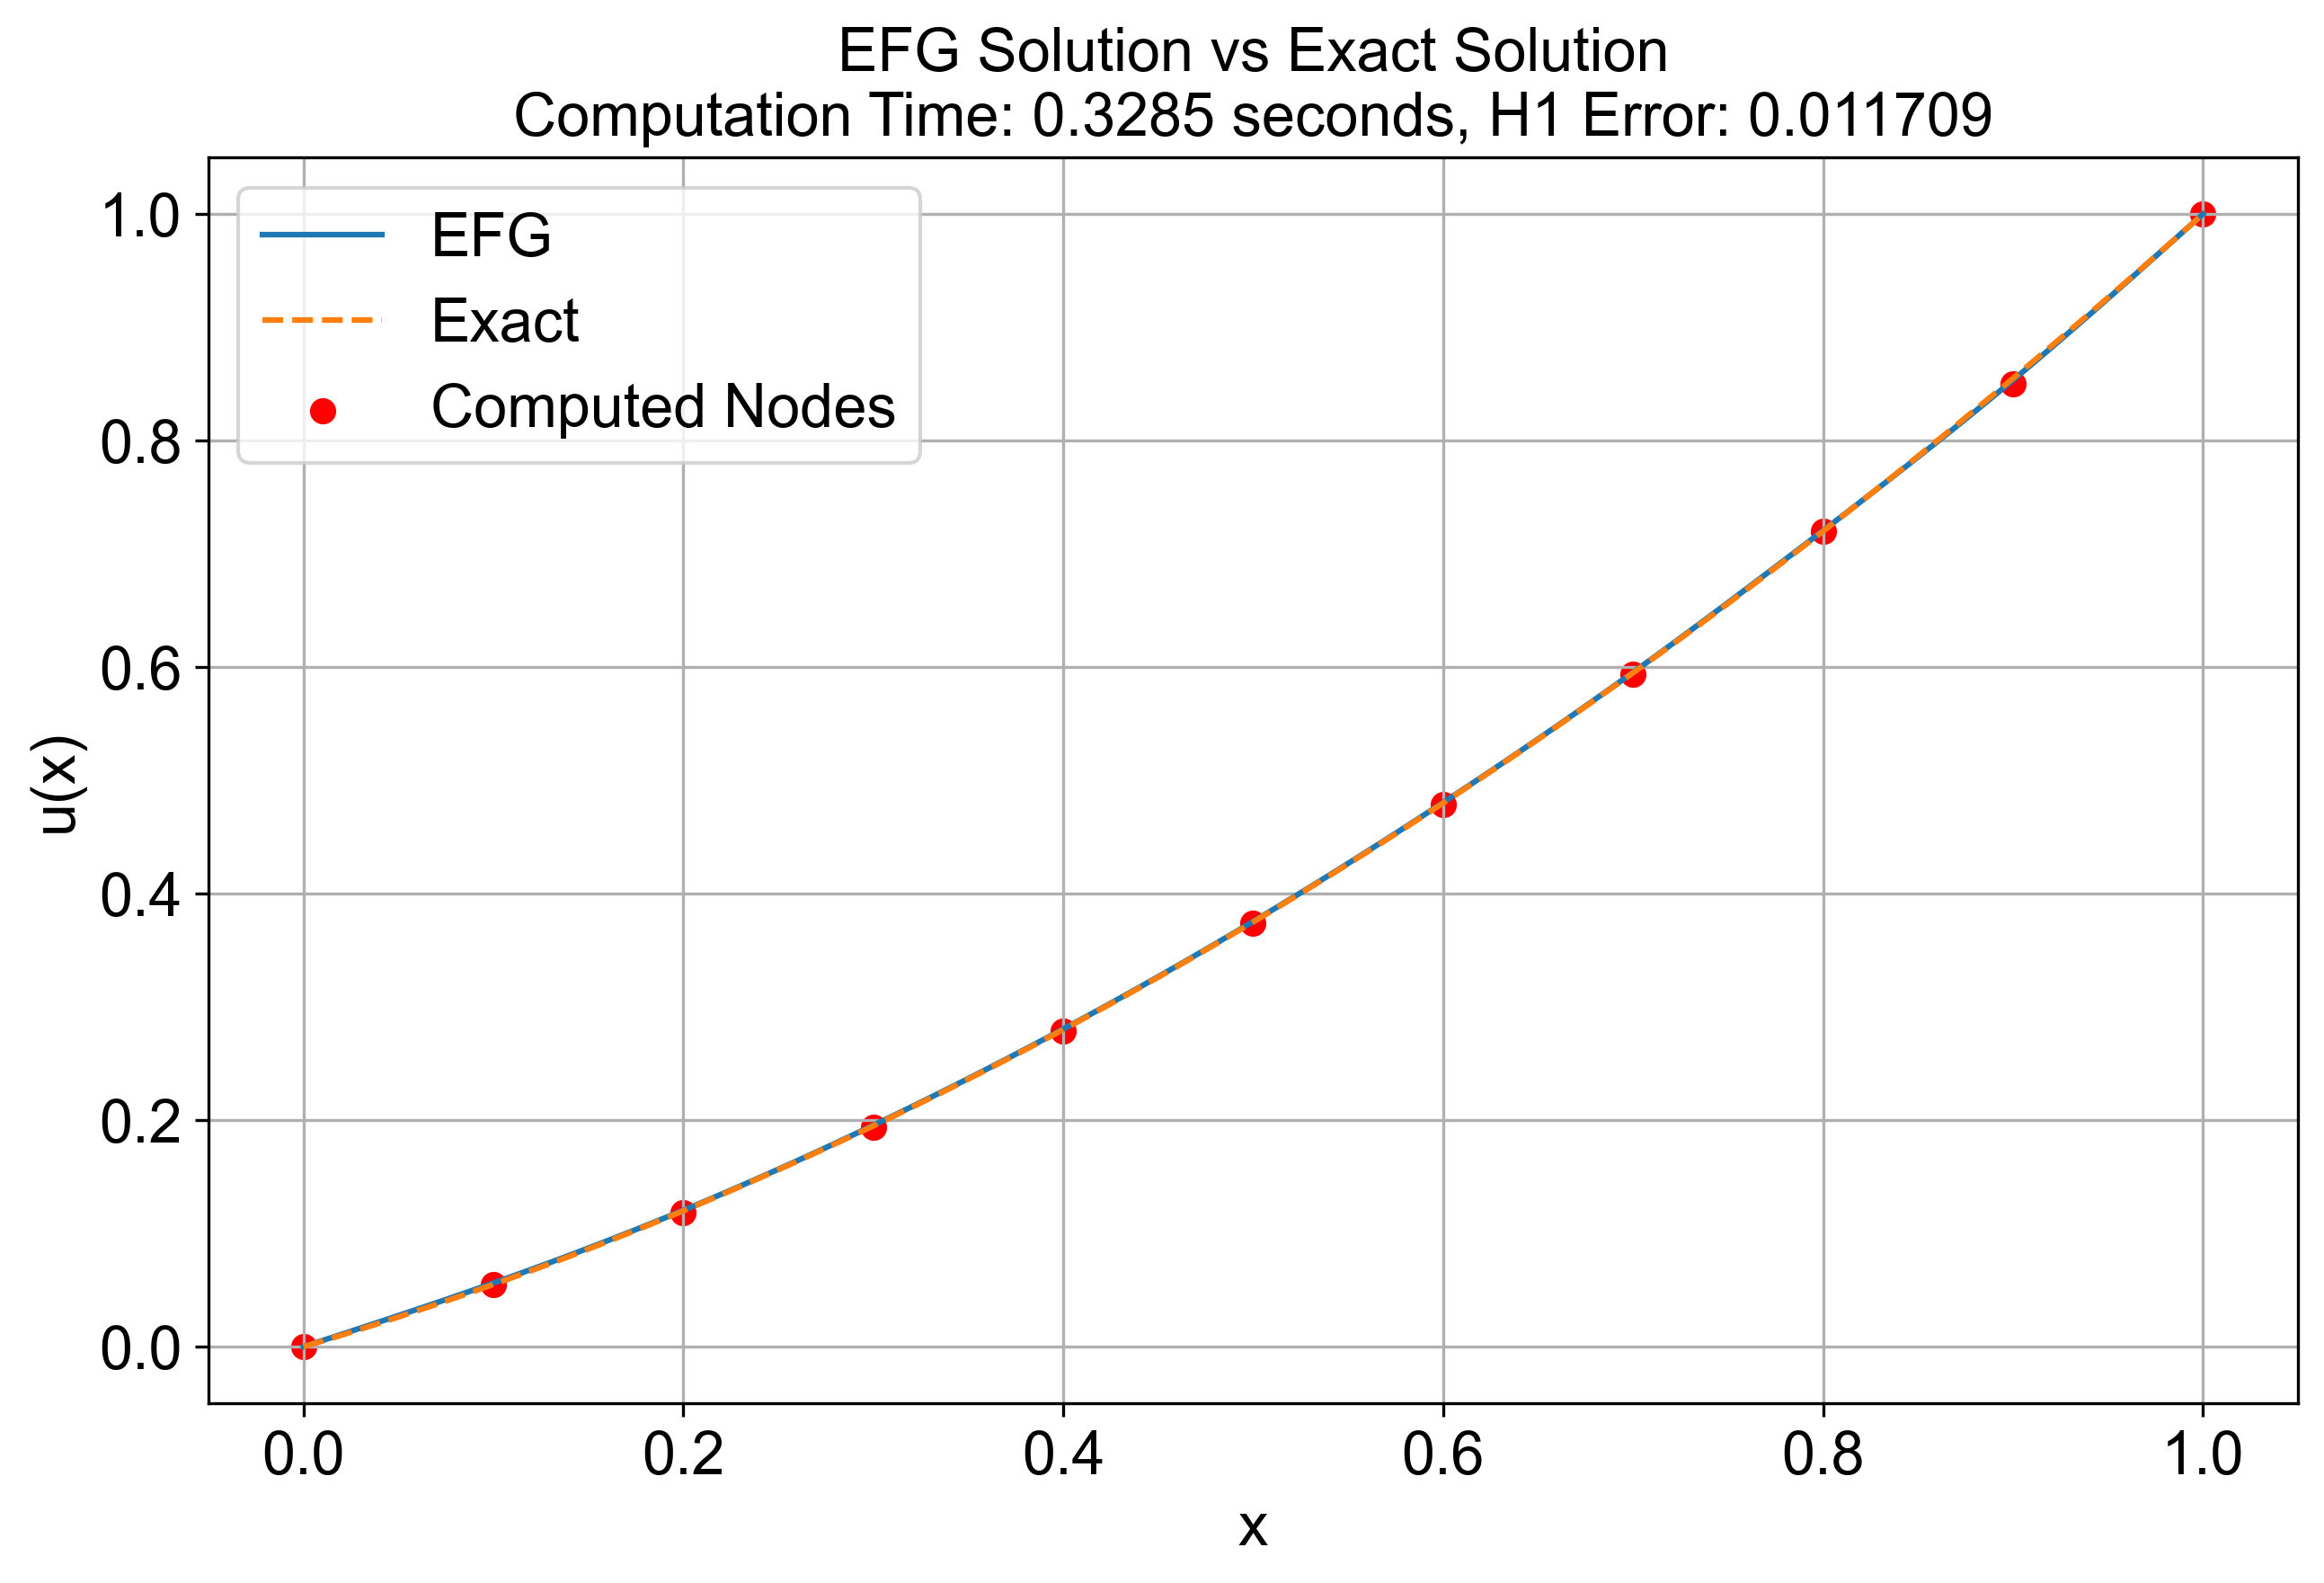
\includegraphics[scale=0.35]{figures/4-1.png} % 进一步减小缩放比例
        \captionof{figure}{基于伽辽金型无网格方法的一维弹性杆问题数值结果}
        \label{CHGraphsettings_fig1_meshfree}
    \end{minipage}
    \hfill
    \begin{minipage}{0.45\textwidth} % 调整为 0.45 以留出间隙
        \centering
        \begin{tabular}{cccc}
            \toprule
            $x$ & $u_{\text{exact}}$ & $u_{\text{computed}}$ & 误差 \\
            \midrule
            0.000 & 0.000000 & 0.000000 & 0.000000 \\
            0.100 & 0.055000 & 0.054726 & 0.000274 \\
            0.200 & 0.120000 & 0.118594 & 0.001406 \\
            0.300 & 0.195000 & 0.193921 & 0.001079 \\
            0.400 & 0.280000 & 0.278816 & 0.001184 \\
            0.500 & 0.375000 & 0.373794 & 0.001206 \\
            0.600 & 0.480000 & 0.478903 & 0.001097 \\
            0.700 & 0.595000 & 0.593458 & 0.001542 \\
            0.800 & 0.720000 & 0.719886 & 0.000114 \\
            0.900 & 0.855000 & 0.850146 & 0.004854 \\
            1.000 & 1.000000 & 1.000000 & 0.000000 \\
            \bottomrule
        \end{tabular}
        \captionof{table}{解析解与计算解的对比}
        \label{tab:exact_vs_computed}
    \end{minipage}
\end{figure}
RKPM 方法在简单一维问题上具有较高的精度，绝对误差在 \( x = 0.9 \) 处达到最大值 0.004，平均误差约为 0.001，整体误差保持在 \( 10^{-3} \) 数量级，精度较高。与 Deep 里兹 方法相比 ，RKPM 方法的误差分布较为均匀。但RKPM方法的误差在边界附近（如 \( x = 0.9 \)）较大，而Deep 里兹 方法通过惩罚项能更有效地约束了边界条件。 

\chapter{再生核近似增强深度里兹方法（RKDR方法）}

\section{再生核近似增强}

\subsection{标准深度 里兹 方法}
由第三章可知，标准深度 里兹 方法基于变分原理求解PDE，其核心是将试探函数表示为神经网络\eqref{eq:network_output}\(u_{\theta}(x) = W_n h_{n-1} + b_n\),记作：
\begin{equation}
u_\theta(x) = NN(x; \theta),
\end{equation}

其中 \(NN(x; \theta)\) 是一个全连接神经网络，输入为空间坐标 \(x \in \mathbb{R}^d\)，输出为标量 \(u_\theta(x)\)，\(\theta\) 是网络参数。深度里兹法的本质在于利用神经网络的通用逼近能力，通过最小化能量泛函来近似 PDE 的解。
\begin{comment}
对于泊松方程 \(-\nabla^2 u = f\)，其损失函数为：
\begin{equation}
L(\theta) = \int_\Omega \left[ \frac{1}{2} |\nabla u_\theta|^2 - f u_\theta \right] d\Omega + \lambda \int_{\partial \Omega} (u_\theta - g)^2 ds,
\end{equation}
其中第一项是体能量，第二项是边界惩罚，\(\lambda\) 是惩罚系数。能量积分通过数值采样（如蒙特卡洛方法）近似，梯度 \(\nabla u_\theta\) 由自动求导计算。
\end{comment}
但其依赖全局坐标 \(x\)，难以捕捉解的局部几何特性，同时通过惩罚项强制满足边界条件可能导致边界处误差较大。因此解的逼近可能需要更深的网络或更长的训练时间。这些不足促使了增强型方法的提出。


\subsection{增强机制：MLS 形函数}
增强型深度 里兹 方法引入移动最小二乘法（MLS）形函数 \(\Psi(x)\) 来改进试探函数。MLS 形函数已在第四章详细推导，这里简述其构造：
给定节点集 \(\{x_j\}_{j=1}^N\)，形函数定义为：
\begin{equation}
u_h(x) = \sum_{j=1}^N \Psi_j(x) u_j,
\end{equation}
满足单位分解性 \(\sum_{j=1}^N \Psi_j(x) = 1\)。其计算简化为：
\begin{equation}
\Psi(x) = p^T(x, x) A^{-1}(x) B(x),
\end{equation}

形函数 \(\Psi(x)\) 的输出形状为 \((batch\_size, N)\)，表示 \(x\) 对每个节点的插值权重。
\begin{comment}
其中：
线性基函数\(p(x_j, x)=[1, (x_j - x)/s]\)，支持域尺度\(s\) 
三次样条核函数\(\phi(r)\) 
\(A(x) = \sum_{j=1}^N \phi_j(x) p(x_j, x) p^T(x_j, x)\)，\(B(x) = [\phi_1(x) p(x_1, x), \dots, \phi_N(x) p(x_N, x)]\)。\\
\end{comment}
\subsection{神经网络模块与特征拼接}
增强型 里兹 方法的核心在于通过特征拼接整合 MLS 形函数与神经网络。试探函数构造为：
\begin{equation}
u_\theta(x) = NN(z(x); \theta), \quad z(x) = [x, \Psi(x)],
\end{equation}
其中 \(z(x)\) 是增强输入特征，\(\oplus\) 表示拼接操作。


原始输入 \(x\) 的形状为 \((batchsize, d)\)，在 \(d=1\) 的情况下为 \((batchsize, 1)\)，表示采样点的坐标，提供全局位置信息。形函数 \(\Psi(x)\) 的形状为 \((batchsize, N)\)，其中每个元素 \(\Psi_j(x)\) 表示 \(x\) 受节点 \(x_j\) 的影响程度，编码了局部几何特性。拼接过程在张量维度上沿特征轴（第 1 维）连接，形式为：
\begin{equation}
z(x) = [x_1, \Psi_1(x), \Psi_2(x), \dots, \Psi_N(x)],
\end{equation}
其中 \(x_1\) 是 \(x\) 的第 1 维坐标（在一维情况下）。对于批量输入，\(z(x)\) 的形状为 \((batchsize, 1 + N)\)。\(x\) 提供全局上下文，确保网络感知整体空间位置， \(\Psi(x)\) 引入局部插值信息，使网络能够感知离散节点的分布以及支持域内的几何关系。拼接后的 \(z(x)\) 是一个复合特征向量，融合了全局和局部信息，从而增强了网络的表达能力。这种增强机制通过 \(\Psi(x)\) 的紧支撑性使网络对 \(x\) 附近节点的贡献更敏感，改善局部解的精度，同时形函数的单位分解性有助于将边界条件嵌入解中，减少对惩罚项的依赖。

增强型网络 \(NN(z(x); \theta)\) 的结构包括输入层、隐藏层和输出层。输入层的维度为 \(d + N\)（例如 \(1 + N\)），负责接受 \(z(x)\) 作为输入。隐藏层由 \(L\) 层全连接网络组成，每层宽度为 \(width\)，其计算形式为：
\begin{equation}
h_{l+1} = \tanh(W_l h_l + b_l), \quad h_0 = z(x), \quad l = 0, 1, \dots, L-1,
\end{equation}
其中 \(W_l\) 和 \(b_l\) 是可训练参数，\(\tanh\) 函数提供非线性变换。输出层通过线性投影得到结果，形式为：
\begin{equation}
u_\theta(x) = W_L h_L + b_L,
\end{equation}
输出标量 \(u_\theta(x)\)。这种结构确保了网络能够有效处理增强特征并生成 PDE 的近似解。

\section{模块整合}
增强型试探函数整合了 MLS 和神经网络：
\[
u_\theta(x) = NN([x, \Psi(x)]; \theta),
\]
其中 \(\Psi(x) = p^T(x, x) A^{-1}(x) B(x)\)。这种整合使网络同时具备局部插值（MLS）和全局非线性拟合（神经网络）的能力。

基于 里兹 变分原理，损失函数简化为：
\begin{equation}
\mathcal{L}(\theta) = \frac{1}{N_b} \sum_{i=1}^{N_b} \left[ \frac{1}{2} |\nabla u_\theta(x_i)|^2 - f(x_i) u_\theta(x_i) \right] + \lambda \left[ u_\theta(0)^2 + (u_\theta(1) - 1)^2 \right],
\end{equation}
其中 \(N_b\) 是内部采样点数，\(\lambda\) 是边界惩罚系数。详细推导见伽辽金无网格法章节。

\section{训练算法}
基于增强深度 里兹 方法的大致步骤为\\
1. 初始化：设定网络参数 \(\theta\)、节点集 \(\{x_I\}\)、支持域 \(s\)、学习率 \(\eta\)。\\
2. 采样：随机生成内部点 \(\{x_i^b\}\) 和边界点 \(\{0, 1\}\)。\\
3. 前向传播：计算 \(\Psi(x_i^b)\)，拼接特征 \(z(x_i^b)\)，输出 \(u_\theta(x_i^b)\) 和 \(\nabla u_\theta(x_i^b)\)。\\
4. 损失计算：评估能量项和边界项，得到 \(\mathcal{L}(\theta)\)。\\
5. 优化：通过反向传播更新 \(\theta\)，重复直到收敛。
\begin{comment}
\section{数值结果}
考虑\eqref{eq:poisson_strong}两端固定的一维弹性杆问题，即
\[
    \left\{
    \begin{array}{ll}
        \nabla^2 u - q = 0 & \mathrm{in~} (0, l) \\
        u(0) =u(1)= 0 
    \end{array}
    \right.
    \label{eq:strong_form1}
\]

该问题的解析解为：
\begin{equation}
u(x) = \frac{x^2}{2} + \frac{x}{2}
\label{eq:analytical_solution}
\end{equation}

基于该一维问题构建一个深度神经网络，其中输入和输出维度分别为 1，网络包含宽度为 50 且深度为 1（总层数为 3）的全连接层，采用 $\tanh$ 激活函数；其次，利用 100 个内部采样点和 2 个边界点构造损失函数，其中体积分损失基于拉普拉斯方程的变分形式 $\int_0^1 \left( \frac{1}{2} |\frac{\partial u}{\partial x}|^2 - f u \right) dx$ 近似计算，边界损失通过惩罚系数 1000 强制满足 Dirichlet 边界条件 $u(0)=0$ 和 $u(1)=1$；然后，引入再生核增强模块，采用 11 个均匀分布的节点（间距 0.1）及支持域大小 0.2 的三次样条核函数，计算形状函数并将其与原始输入拼接，增强网络特征表达；最后，采用 Adam 优化器以初始学习率 0.001 并结合步长为 300、衰减因子 0.3 的 StepLR 调度器，在 10000 步训练中通过批量梯度下降优化损失函数，每 10 步记录一次误差，测试阶段则在 100 个积分点上评估 $L^2$ 和 $H^1$ 误差。

\newpage
\subsection{对比Deep 里兹方法}
\subsection*{训练精度对比}
\begin{figure}[htbp]
    \centering
    \begin{subfigure}[b]{0.45\textwidth}
        \centering
        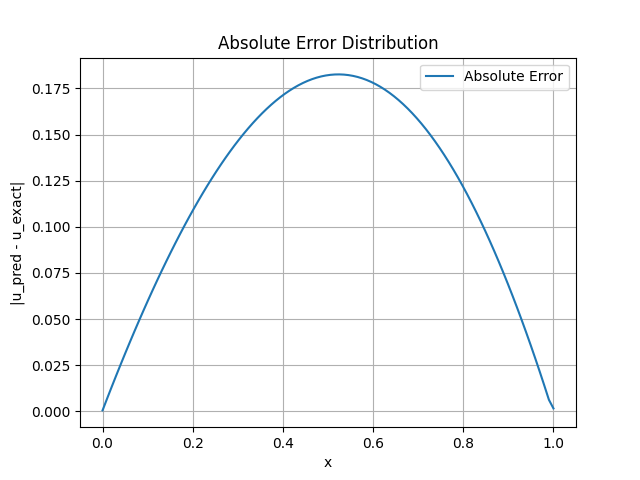
\includegraphics[width=\textwidth, height=6cm, keepaspectratio]{figures/3-1-4.png}
        \caption{深度里兹法1000步绝对误差}
        \label{fig:deepritz_solutions}
    \end{subfigure}
    \hfill
    \begin{subfigure}[b]{0.45\textwidth}
        \centering
        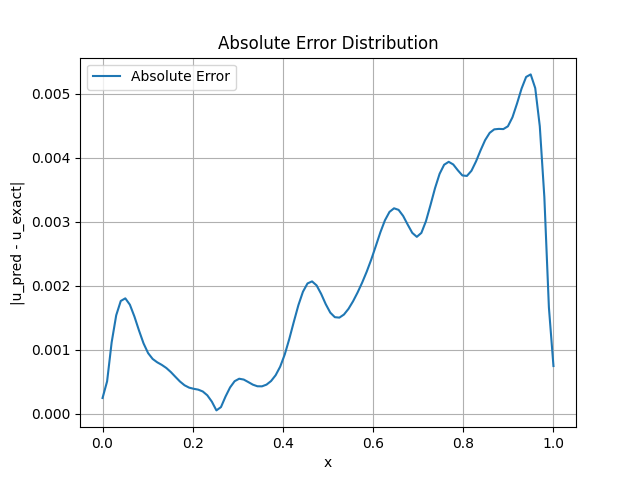
\includegraphics[width=\textwidth, height=6cm, keepaspectratio]{figures/5-1-2.png}
        \caption{再生核增强深度里兹法绝对误差}
        \label{fig:absolute_error}
    \end{subfigure}
    \\
    \begin{subfigure}[b]{0.45\textwidth}
        \centering
        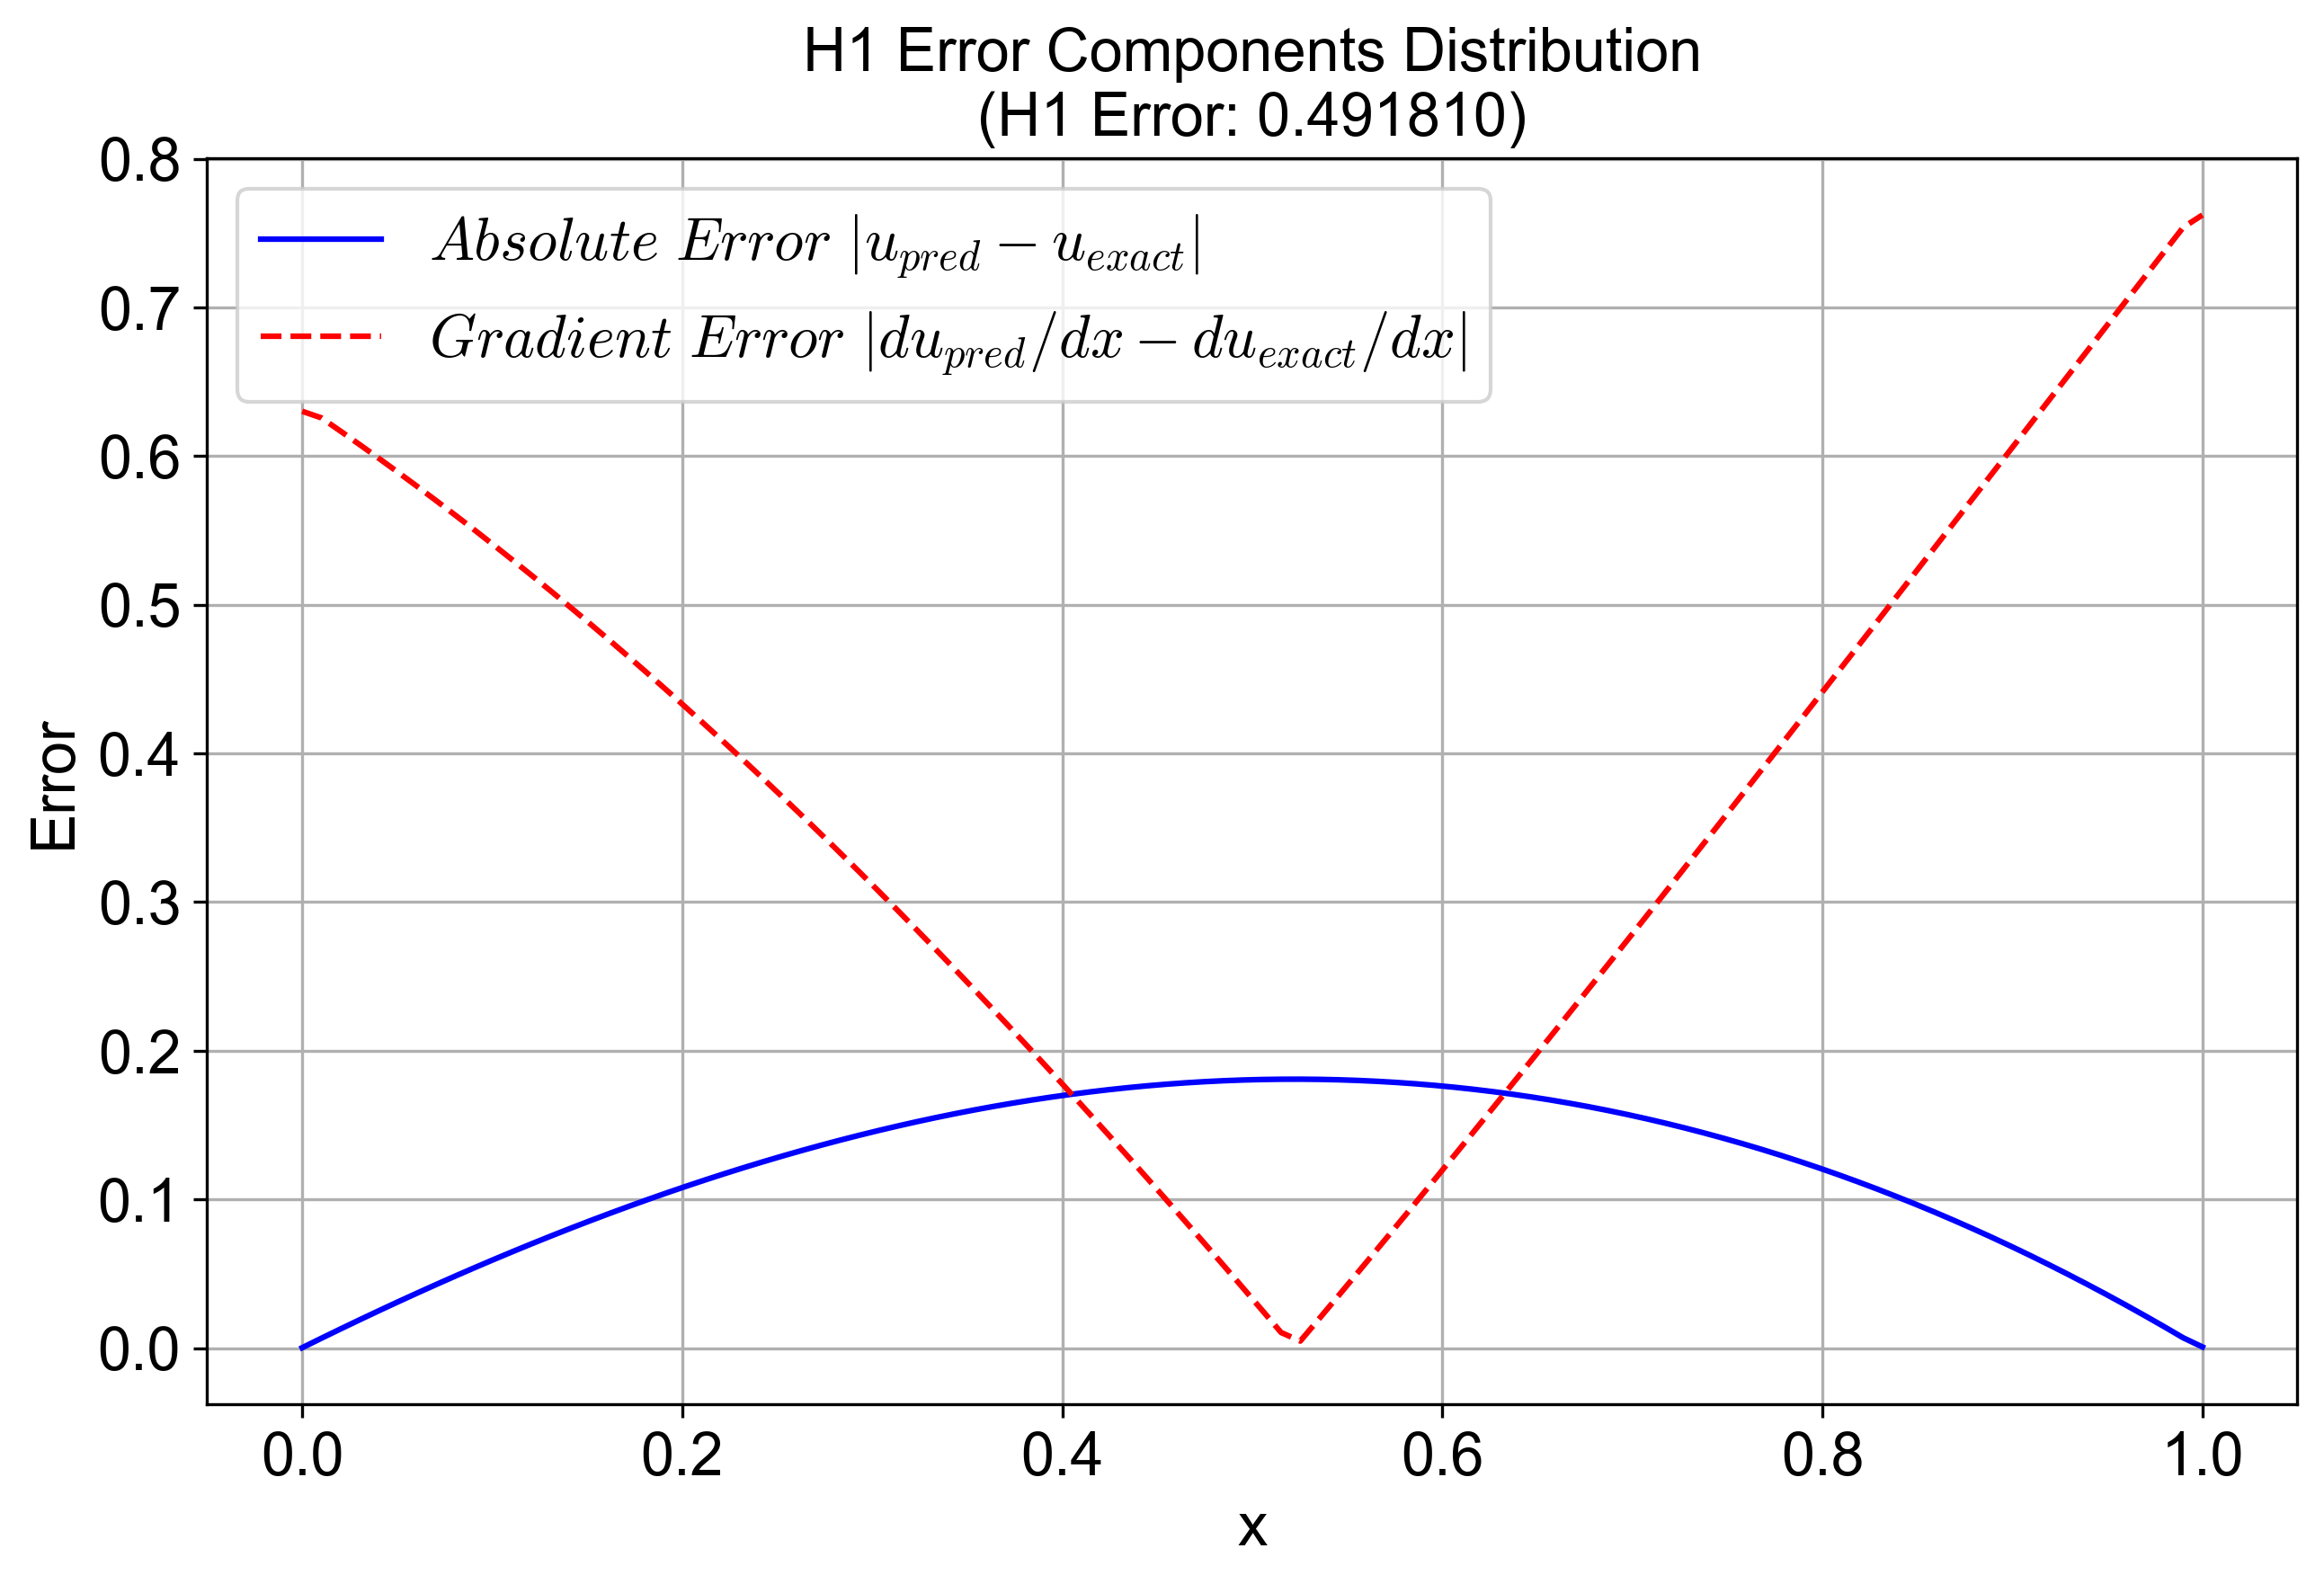
\includegraphics[width=\textwidth, height=6cm, keepaspectratio]{figures/3-1-5.png}
        \caption{深度里兹法1000步H1误差}
        \label{fig:deepritz_solutions}
    \end{subfigure}
    \hfill
    \begin{subfigure}[b]{0.45\textwidth}
        \centering
        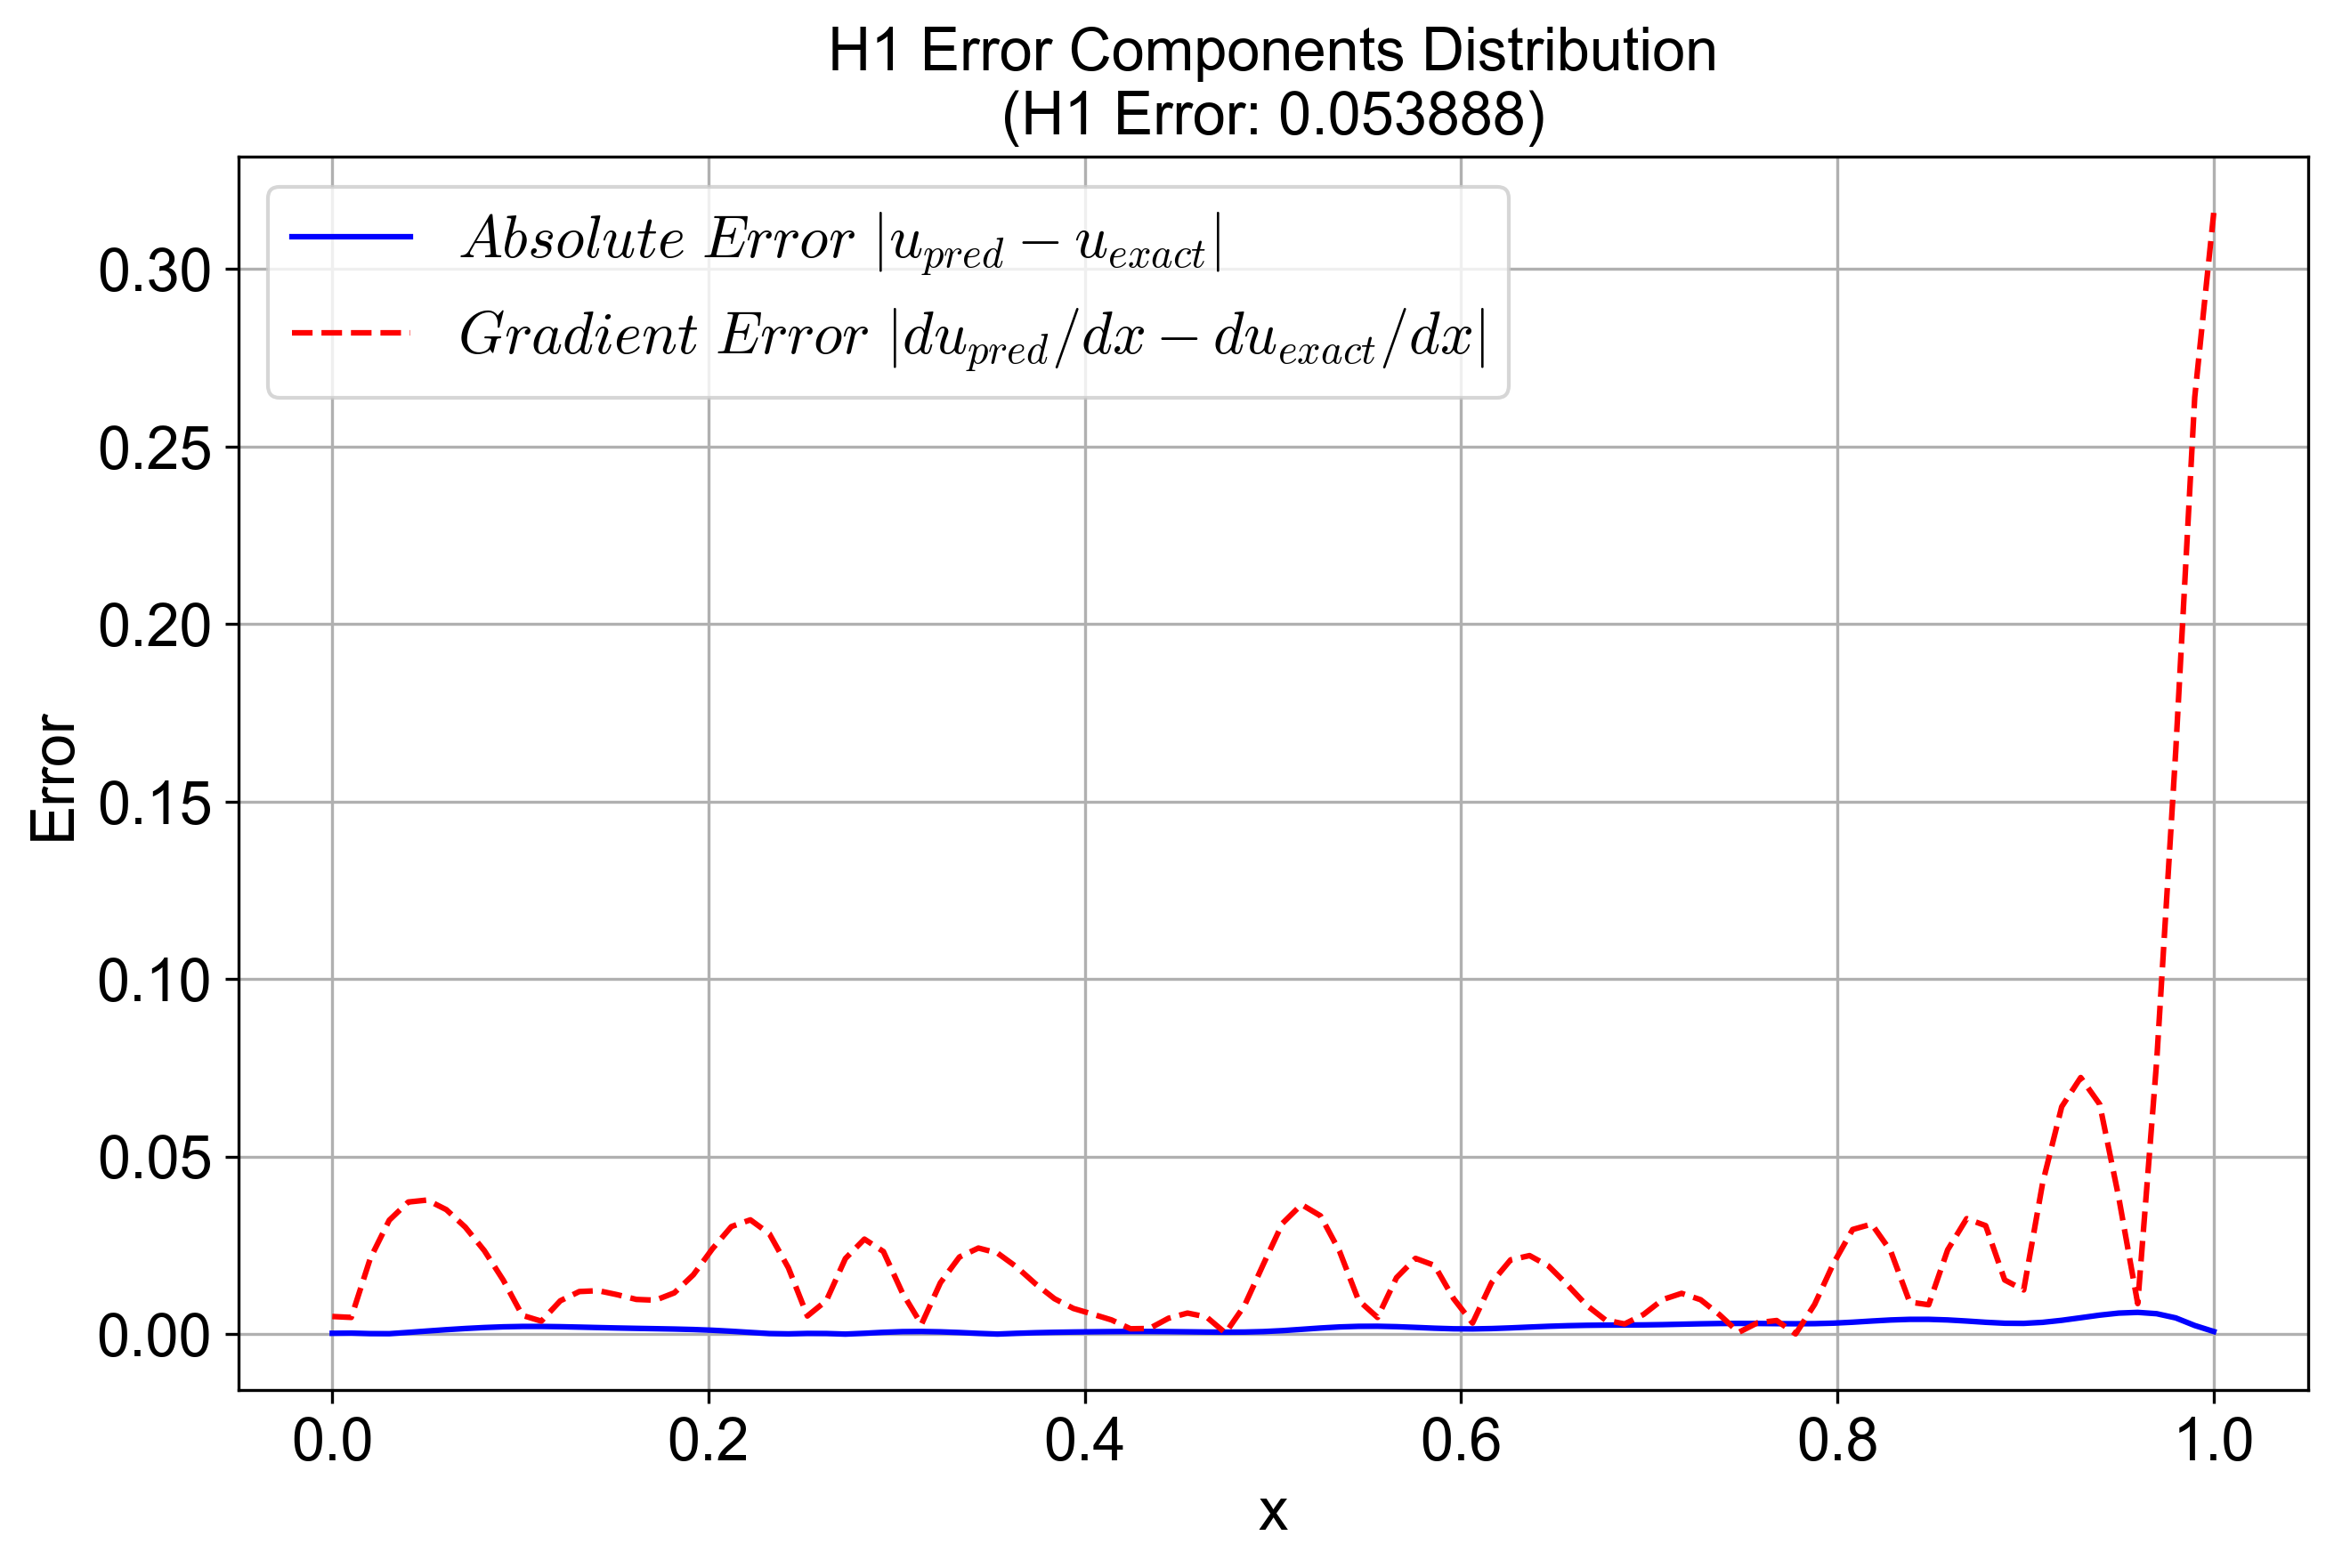
\includegraphics[width=\textwidth, height=6cm, keepaspectratio]{figures/5-1-5.png}
        \caption{再生核增强深度里兹法1000步H1误差}
        \label{fig:absolute_error}
    \end{subfigure}
    \centering
    \caption{1000步误差可视化。}
    \label{fig:combined}
\end{figure}

1000 步训练后深度 里兹 方法的 L2 误差为 0.11，解的整体逼近精度较低。绝对误差分布呈现对称抛物线形状，误差集中在 \( x = 0.2 \) 到 \( x = 0.8 \) 的区域。相比之下，增强深度 里兹 方法将 L2 误差降低至 0.002。绝对误差分布峰值更小，变化平滑，表明引入 EFG 形状函数显著提升了局部逼近能力。

1000步训练后深度 里兹 方法的梯度误差（红色曲线）远高于函数值误差（蓝色曲线），表明模型在捕捉解的导数方面表现较差。再生核增强后 H1 误差显著降低。尽管梯度误差仍高于函数值误差，但其幅度大幅减小，表明 EFG 提升了模型对解导数的逼近能力。

\newpage
\begin{figure}[htbp]
    \centering
    \begin{subfigure}[b]{0.45\textwidth}
        \centering
        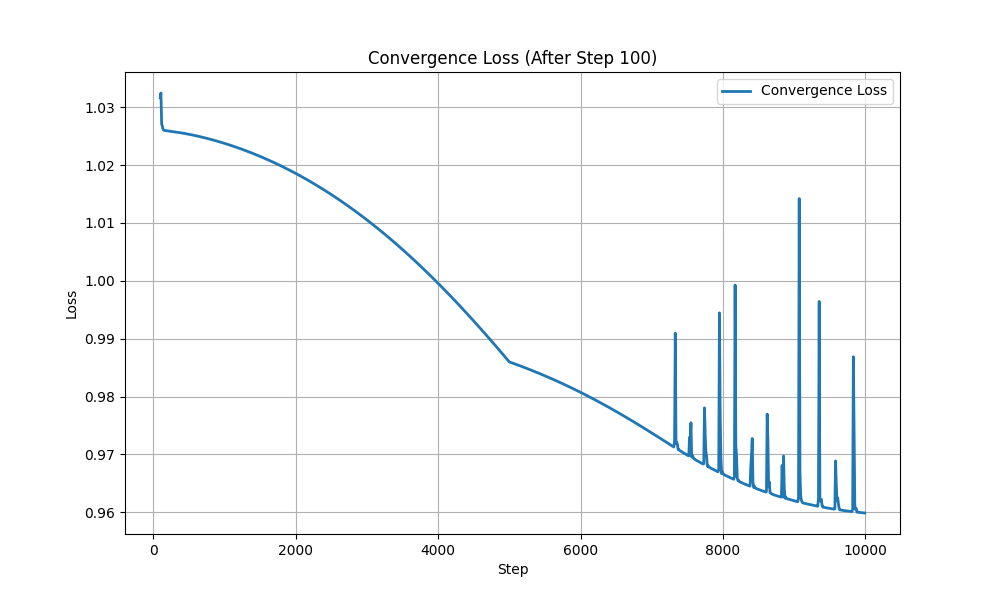
\includegraphics[width=\textwidth, height=6cm, keepaspectratio]{figures/3-2-4.png}
        \caption{深度里兹法10000步L2误差}
        \label{fig:deepritz_solutions}
    \end{subfigure}
    \hfill
    \begin{subfigure}[b]{0.45\textwidth}
        \centering
        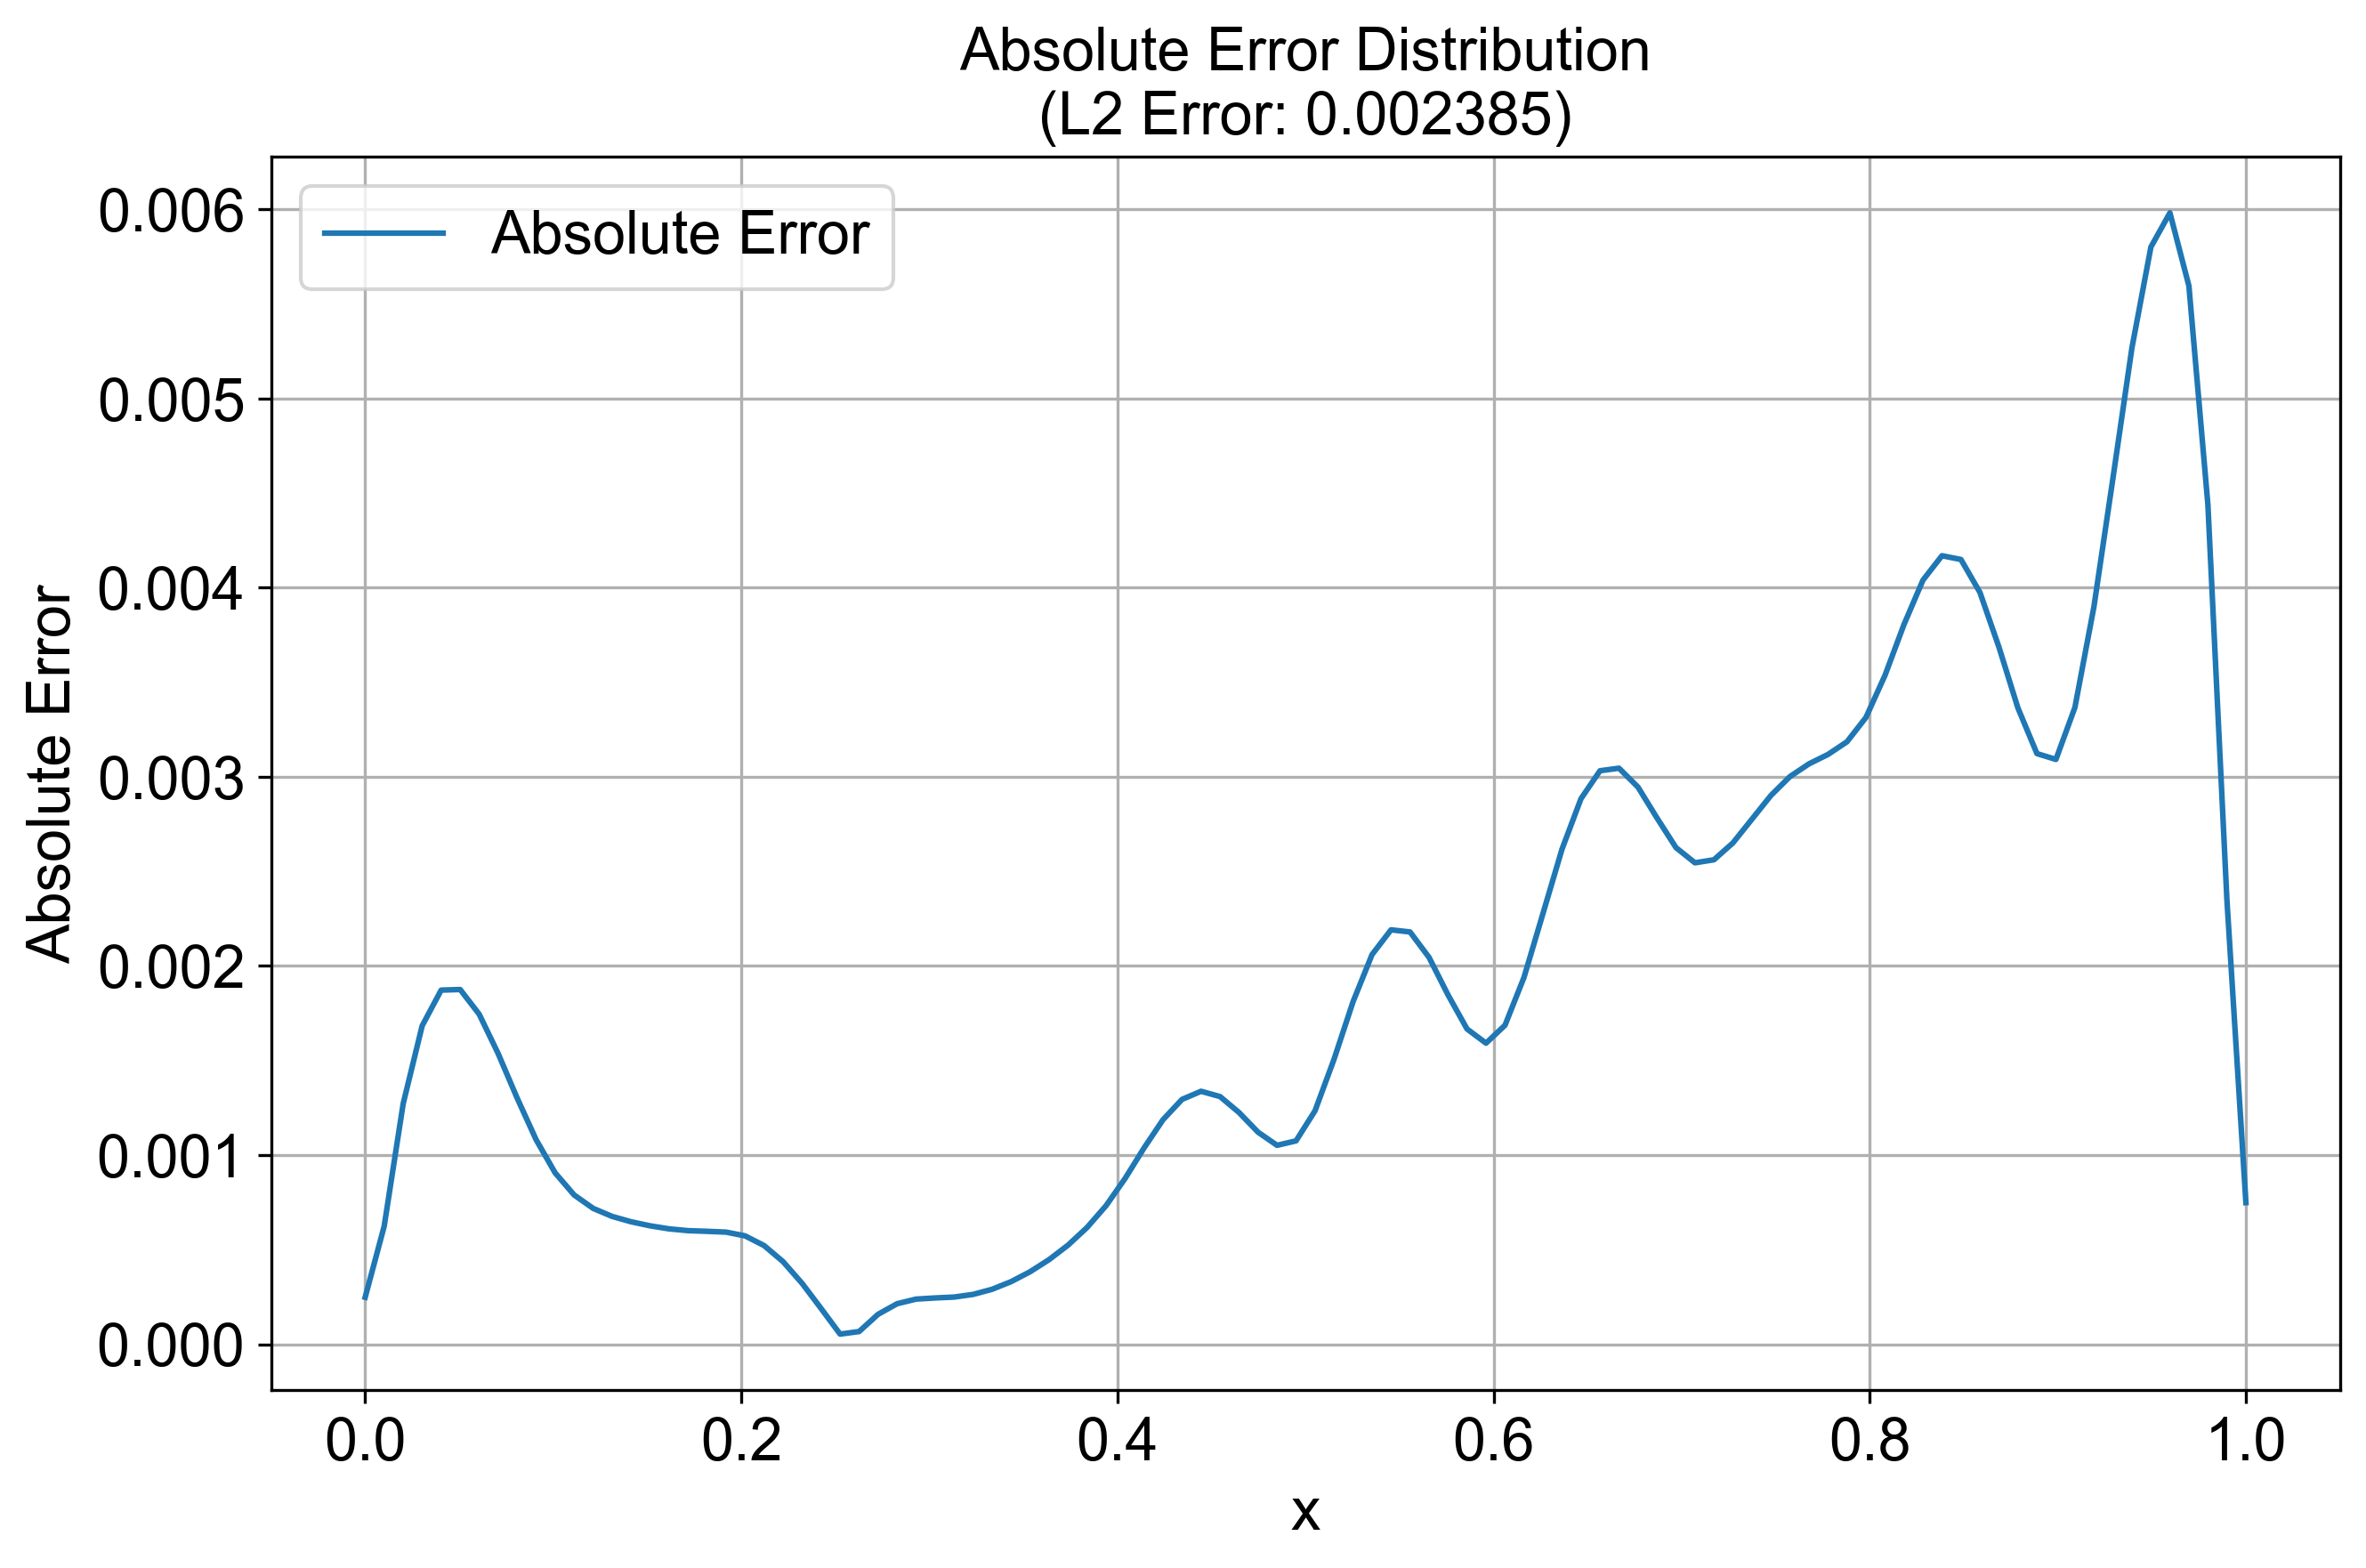
\includegraphics[width=\textwidth, height=6cm, keepaspectratio]{figures/5-2-2.png}
        \caption{再生核增强10000步L2误差}
        \label{fig:absolute_error}
    \end{subfigure}
    \\
    \begin{subfigure}[b]{0.45\textwidth}
        \centering
        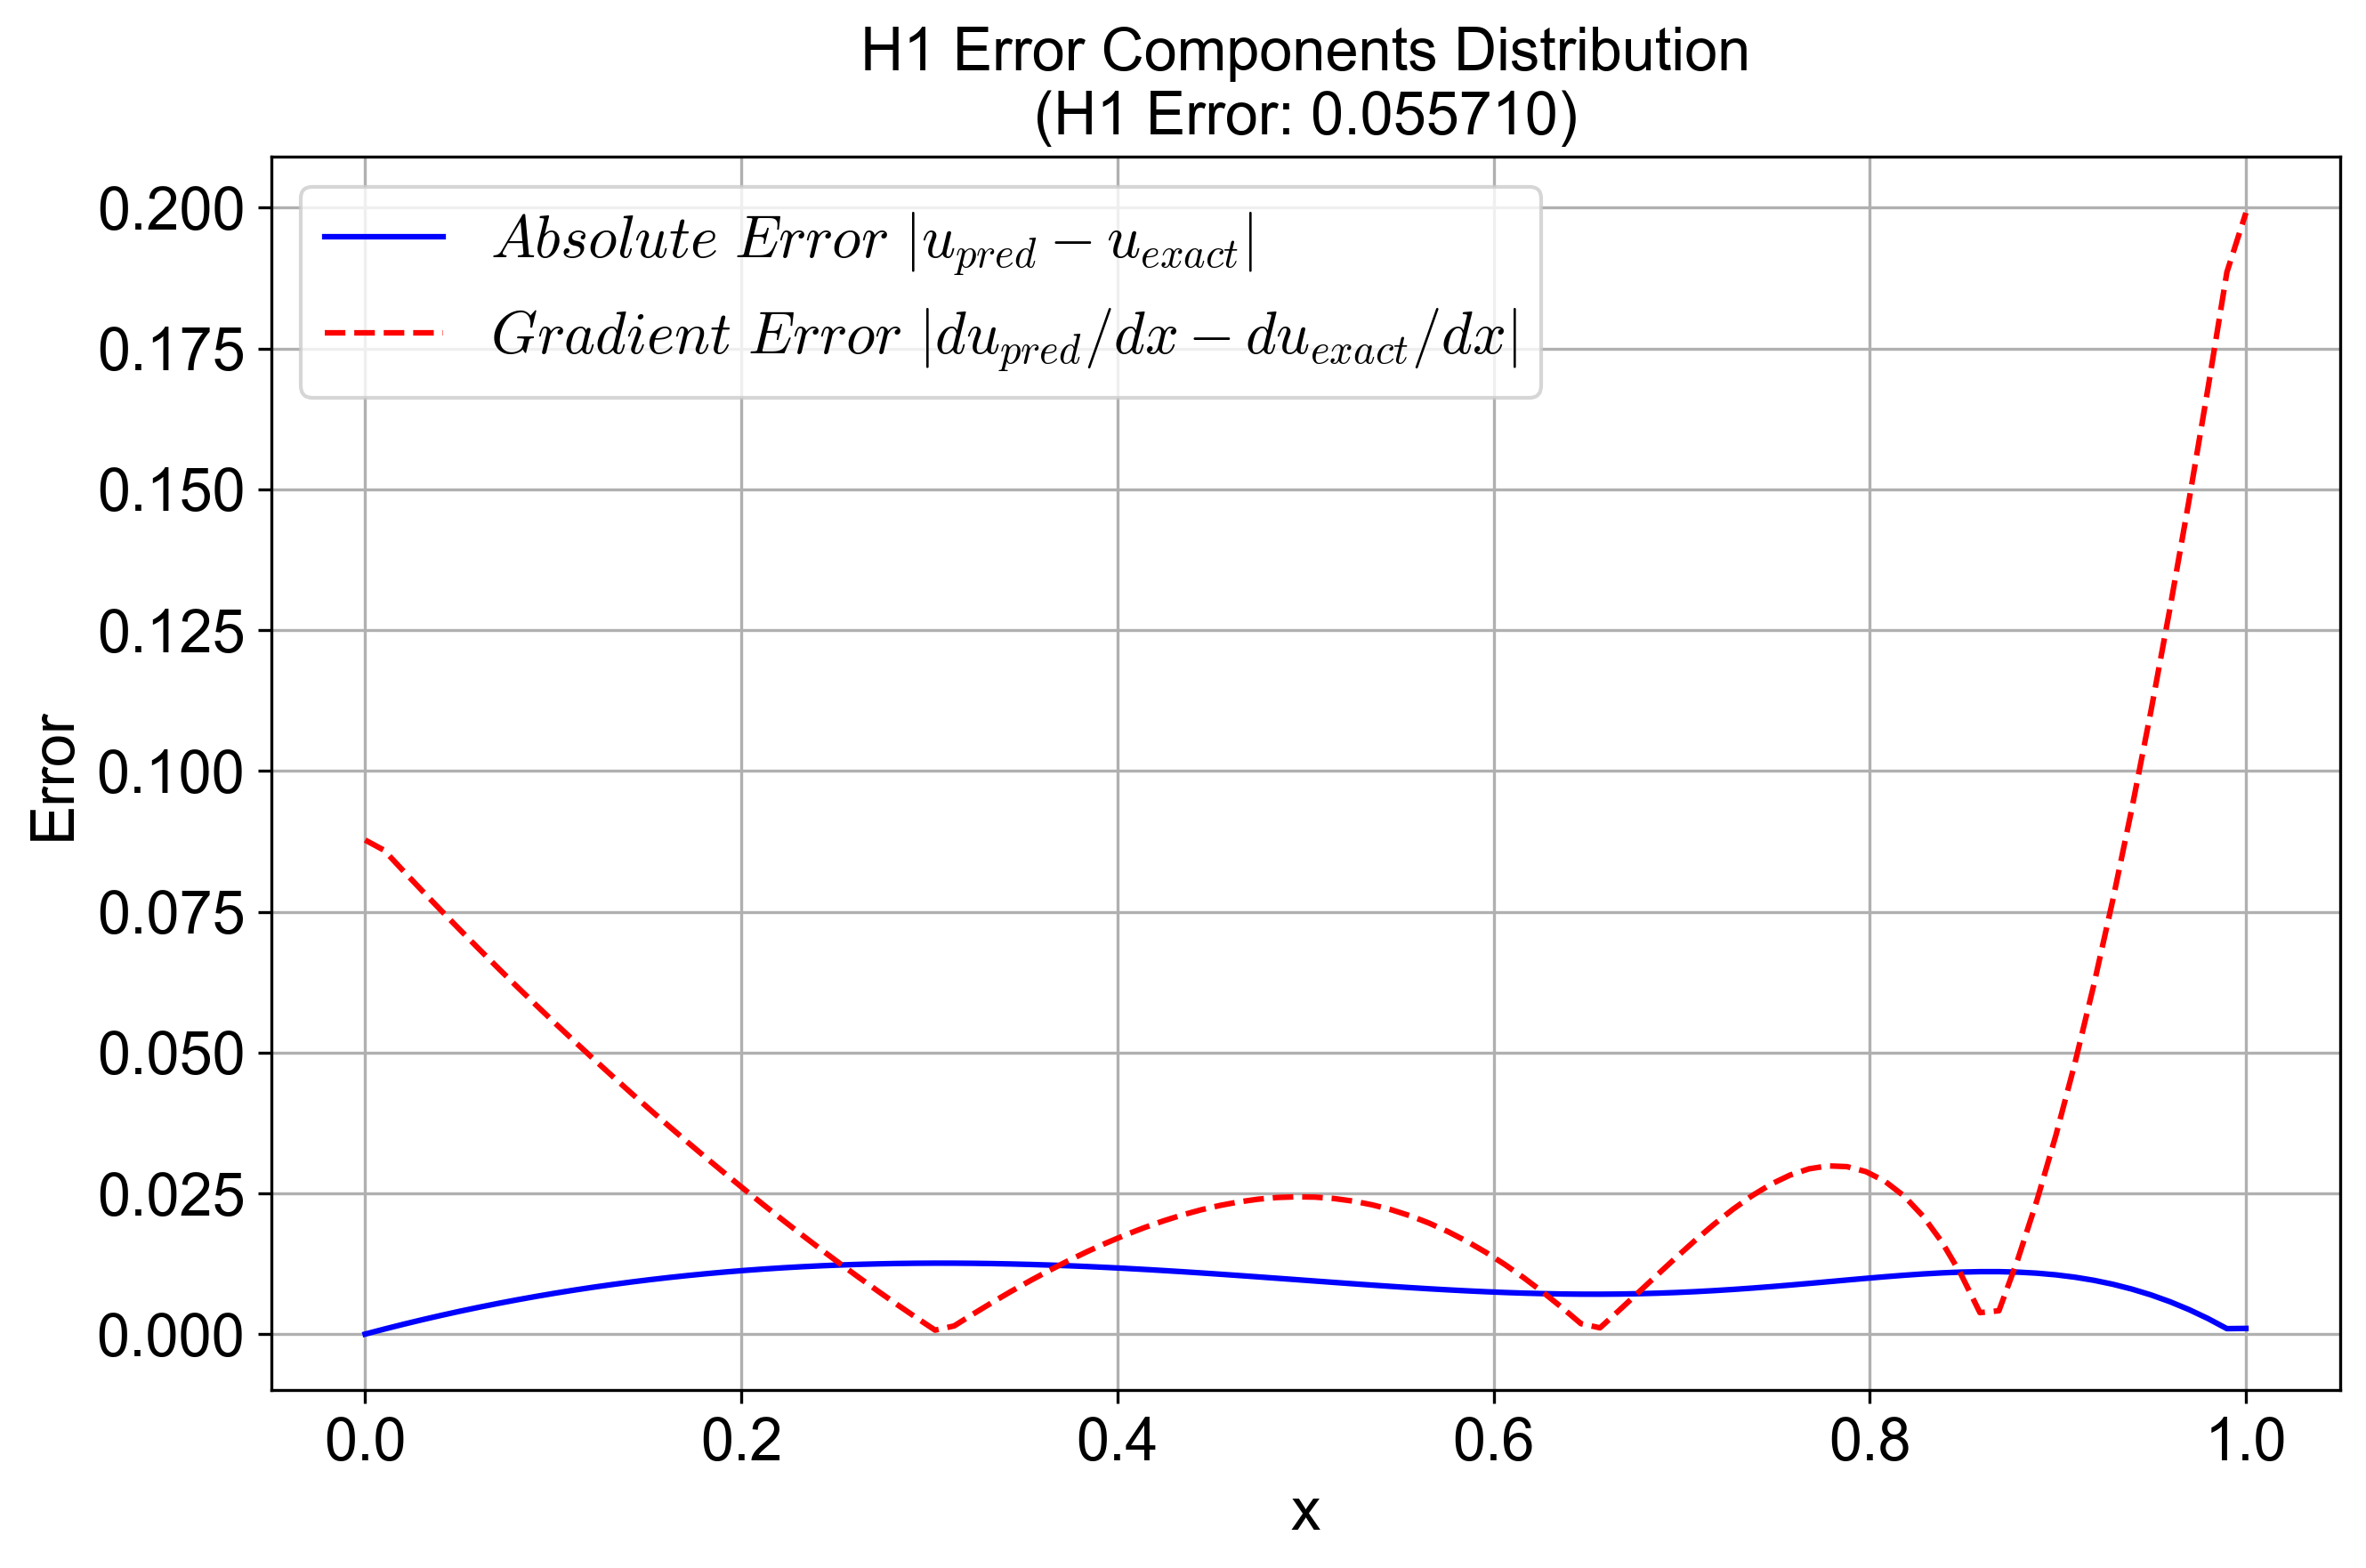
\includegraphics[width=\textwidth, height=6cm, keepaspectratio]{figures/3-2-5.png}
        \caption{深度里兹法10000步H1误差}
        \label{fig:deepritz_solutions}
    \end{subfigure}
    \hfill
    \begin{subfigure}[b]{0.45\textwidth}
        \centering
        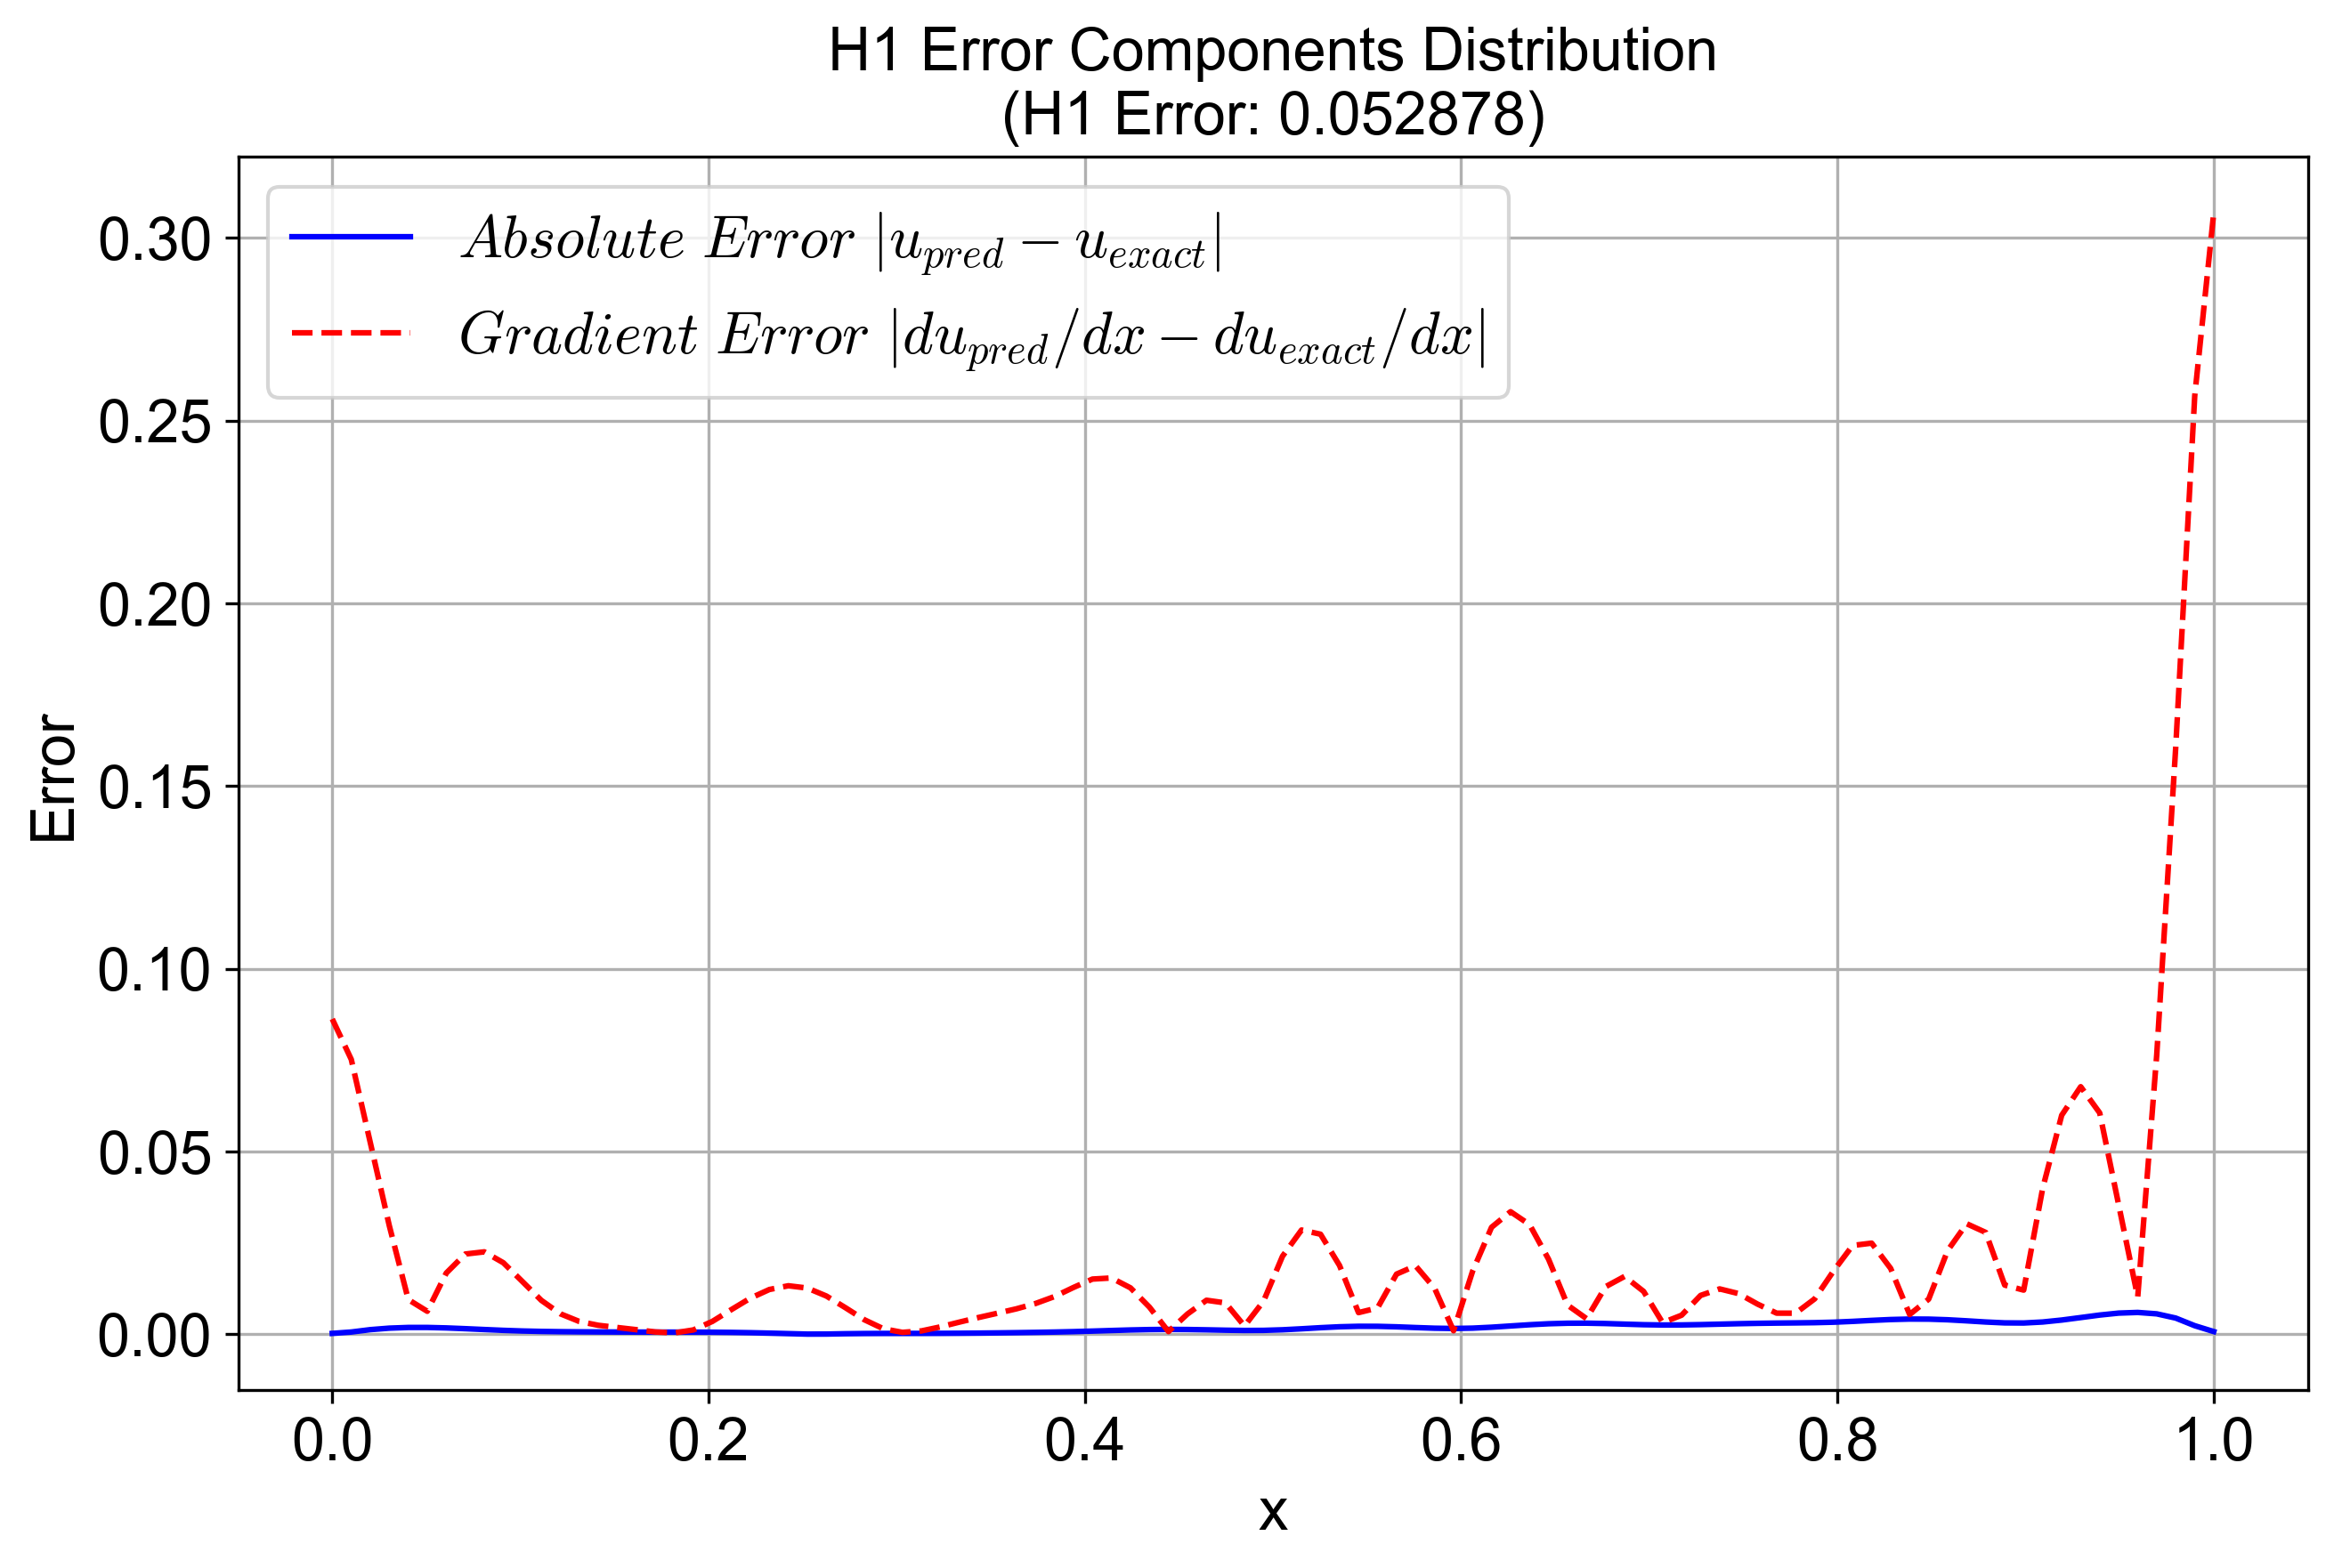
\includegraphics[width=\textwidth, height=6cm, keepaspectratio]{figures/5-2-5.png}
        \caption{再生核增强10000步H1误差}
        \label{fig:absolute_error}
    \end{subfigure}
    \centering
    \caption{10000步误差可视化}
    \label{fig:combined}
\end{figure}

10000 步训练后，Deep里兹 方法的 L2 误差和 H1 误差分别为 0.016 和 0.080，相较 1000 步（0.25 和 0.5）显著降低，但中间区域 L2 误差较大，边界处导数误差显著；RK-Deep里兹 方法的 L2 误差和 H1 误差为 0.0024 和 0.049，相较 1000 步（0.1 和 0.2）显著降低，误差分布波动较多但整体更低，优于 Deep里兹。

\subsection*{误差收敛效果}

\begin{figure}[htbp]
    \centering
    \begin{subfigure}[b]{0.45\textwidth}
        \centering
        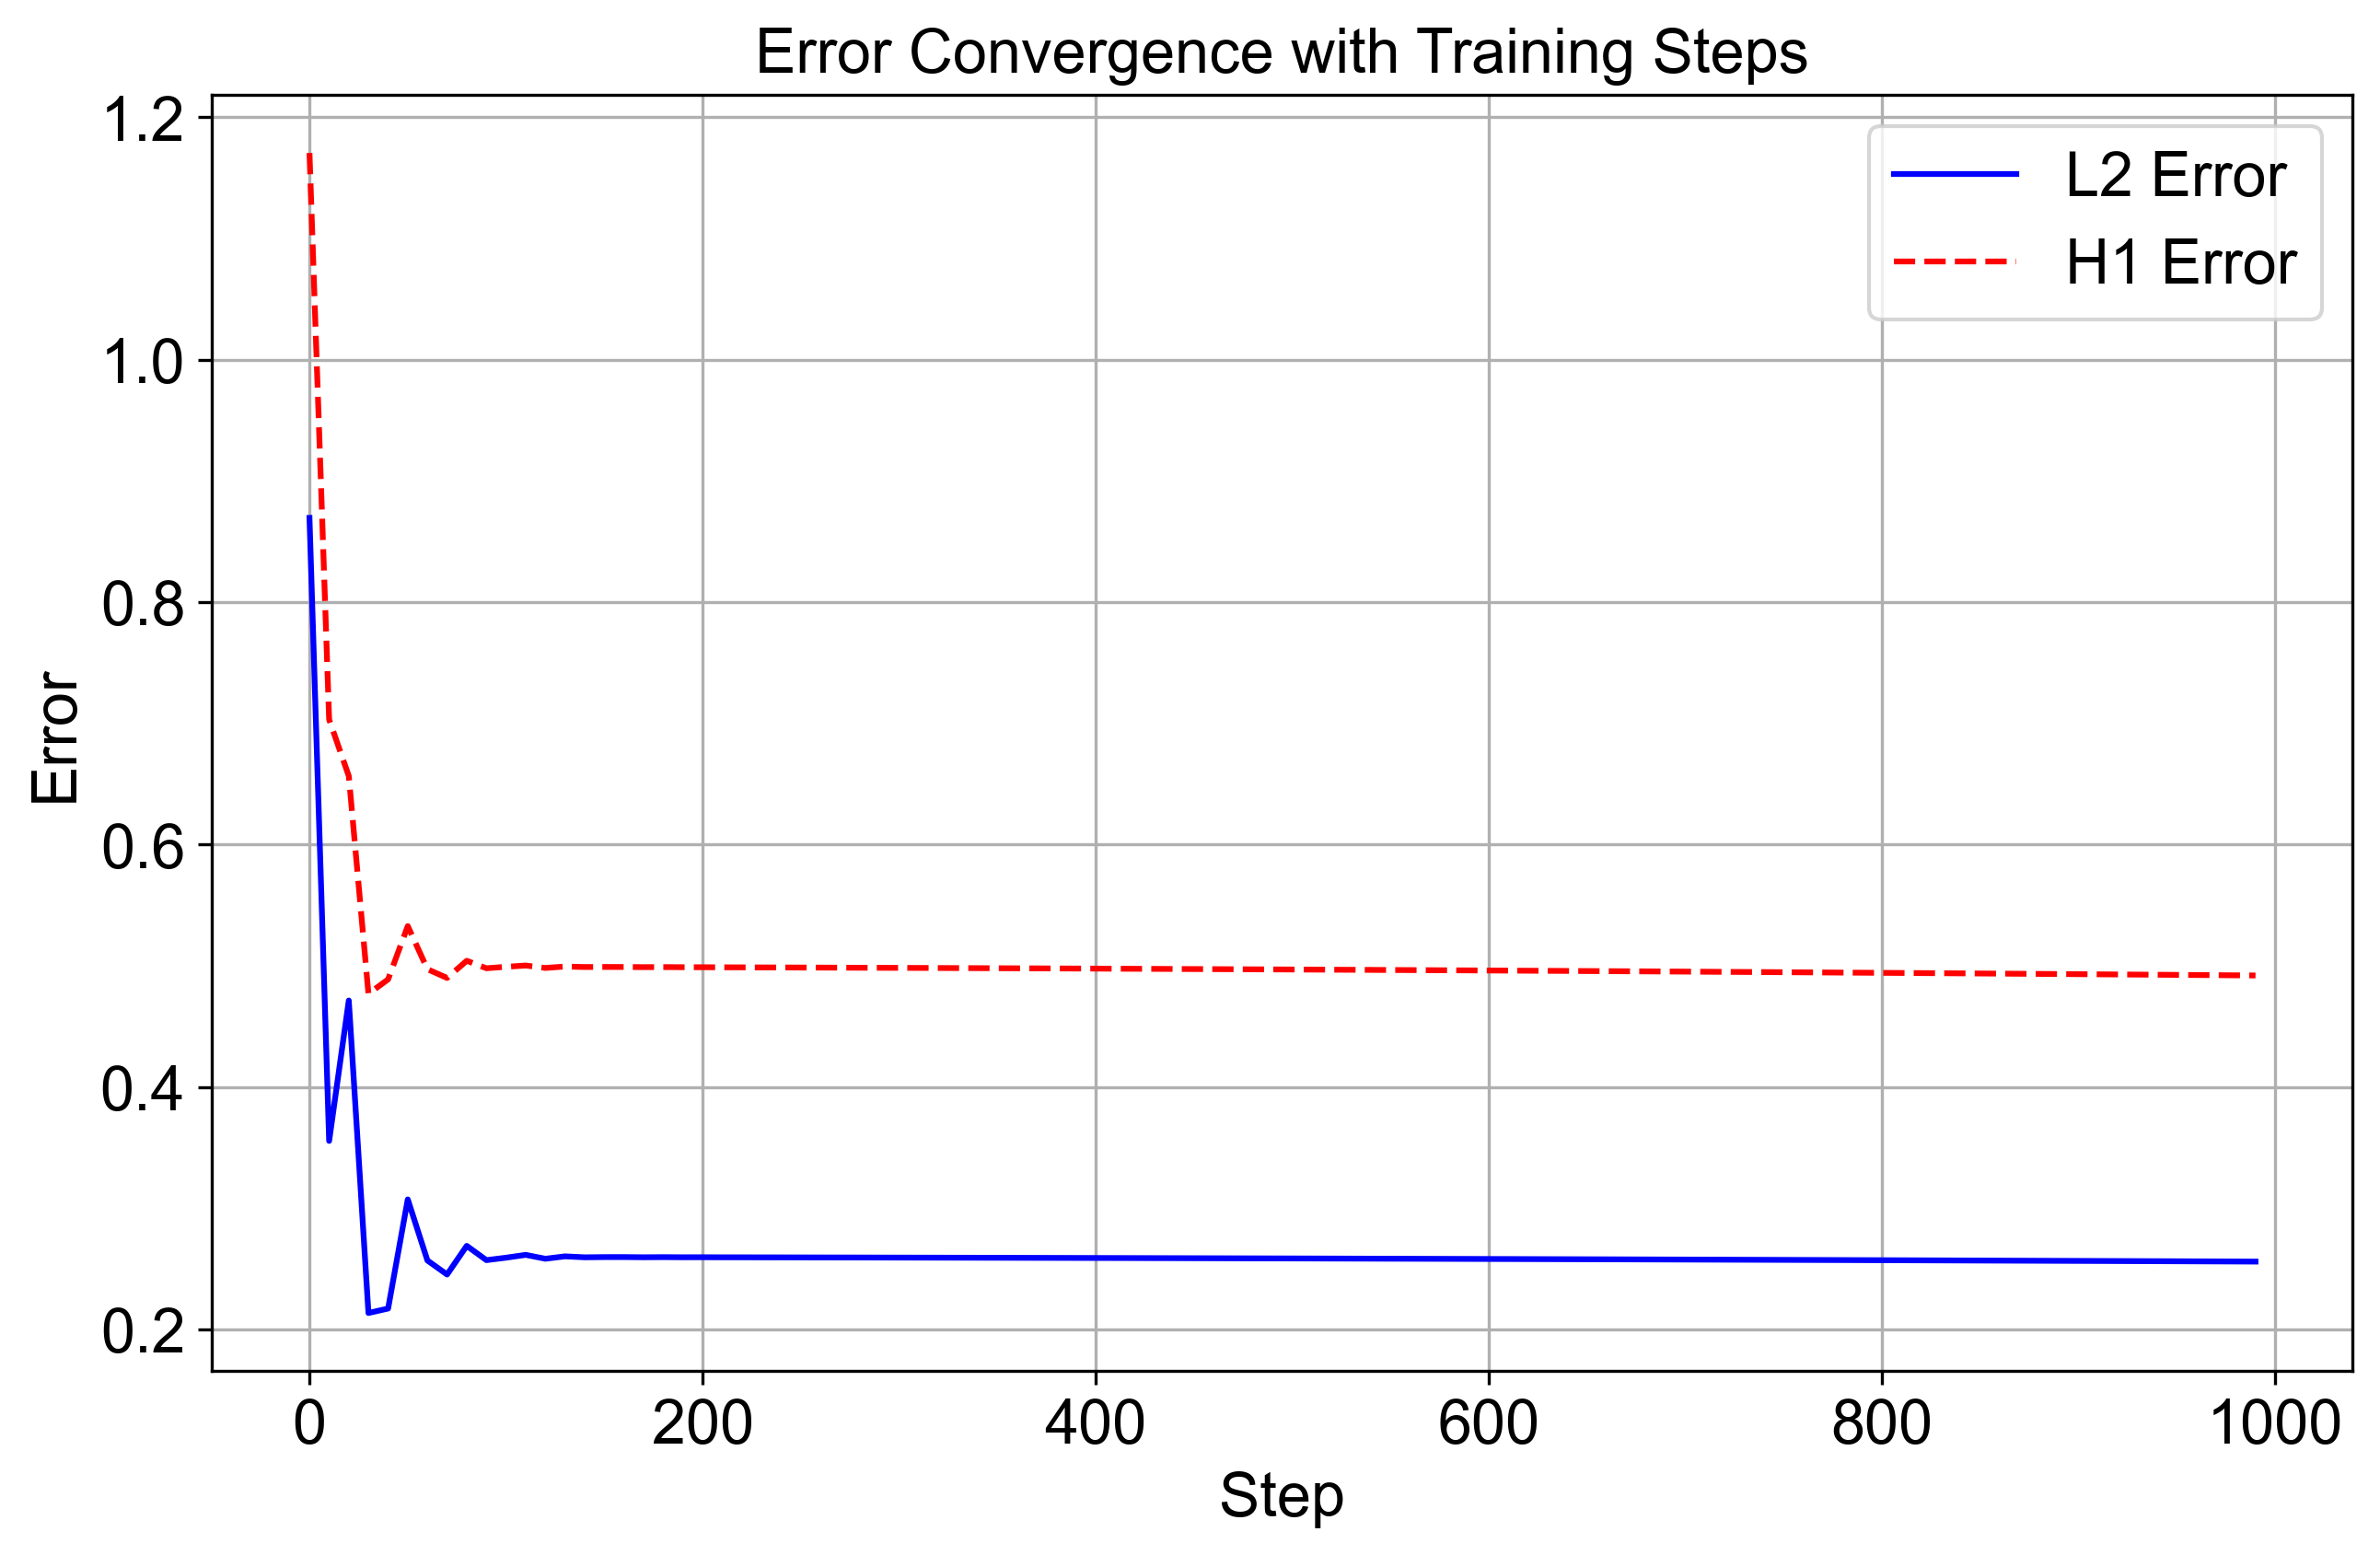
\includegraphics[width=\textwidth, height=6cm, keepaspectratio]{figures/3-1-6.png}
        \caption{深度里兹法1000步误差收敛曲线}
        \label{fig:deepritz_solutions}
    \end{subfigure}
    \hfill
    \begin{subfigure}[b]{0.45\textwidth}
        \centering
        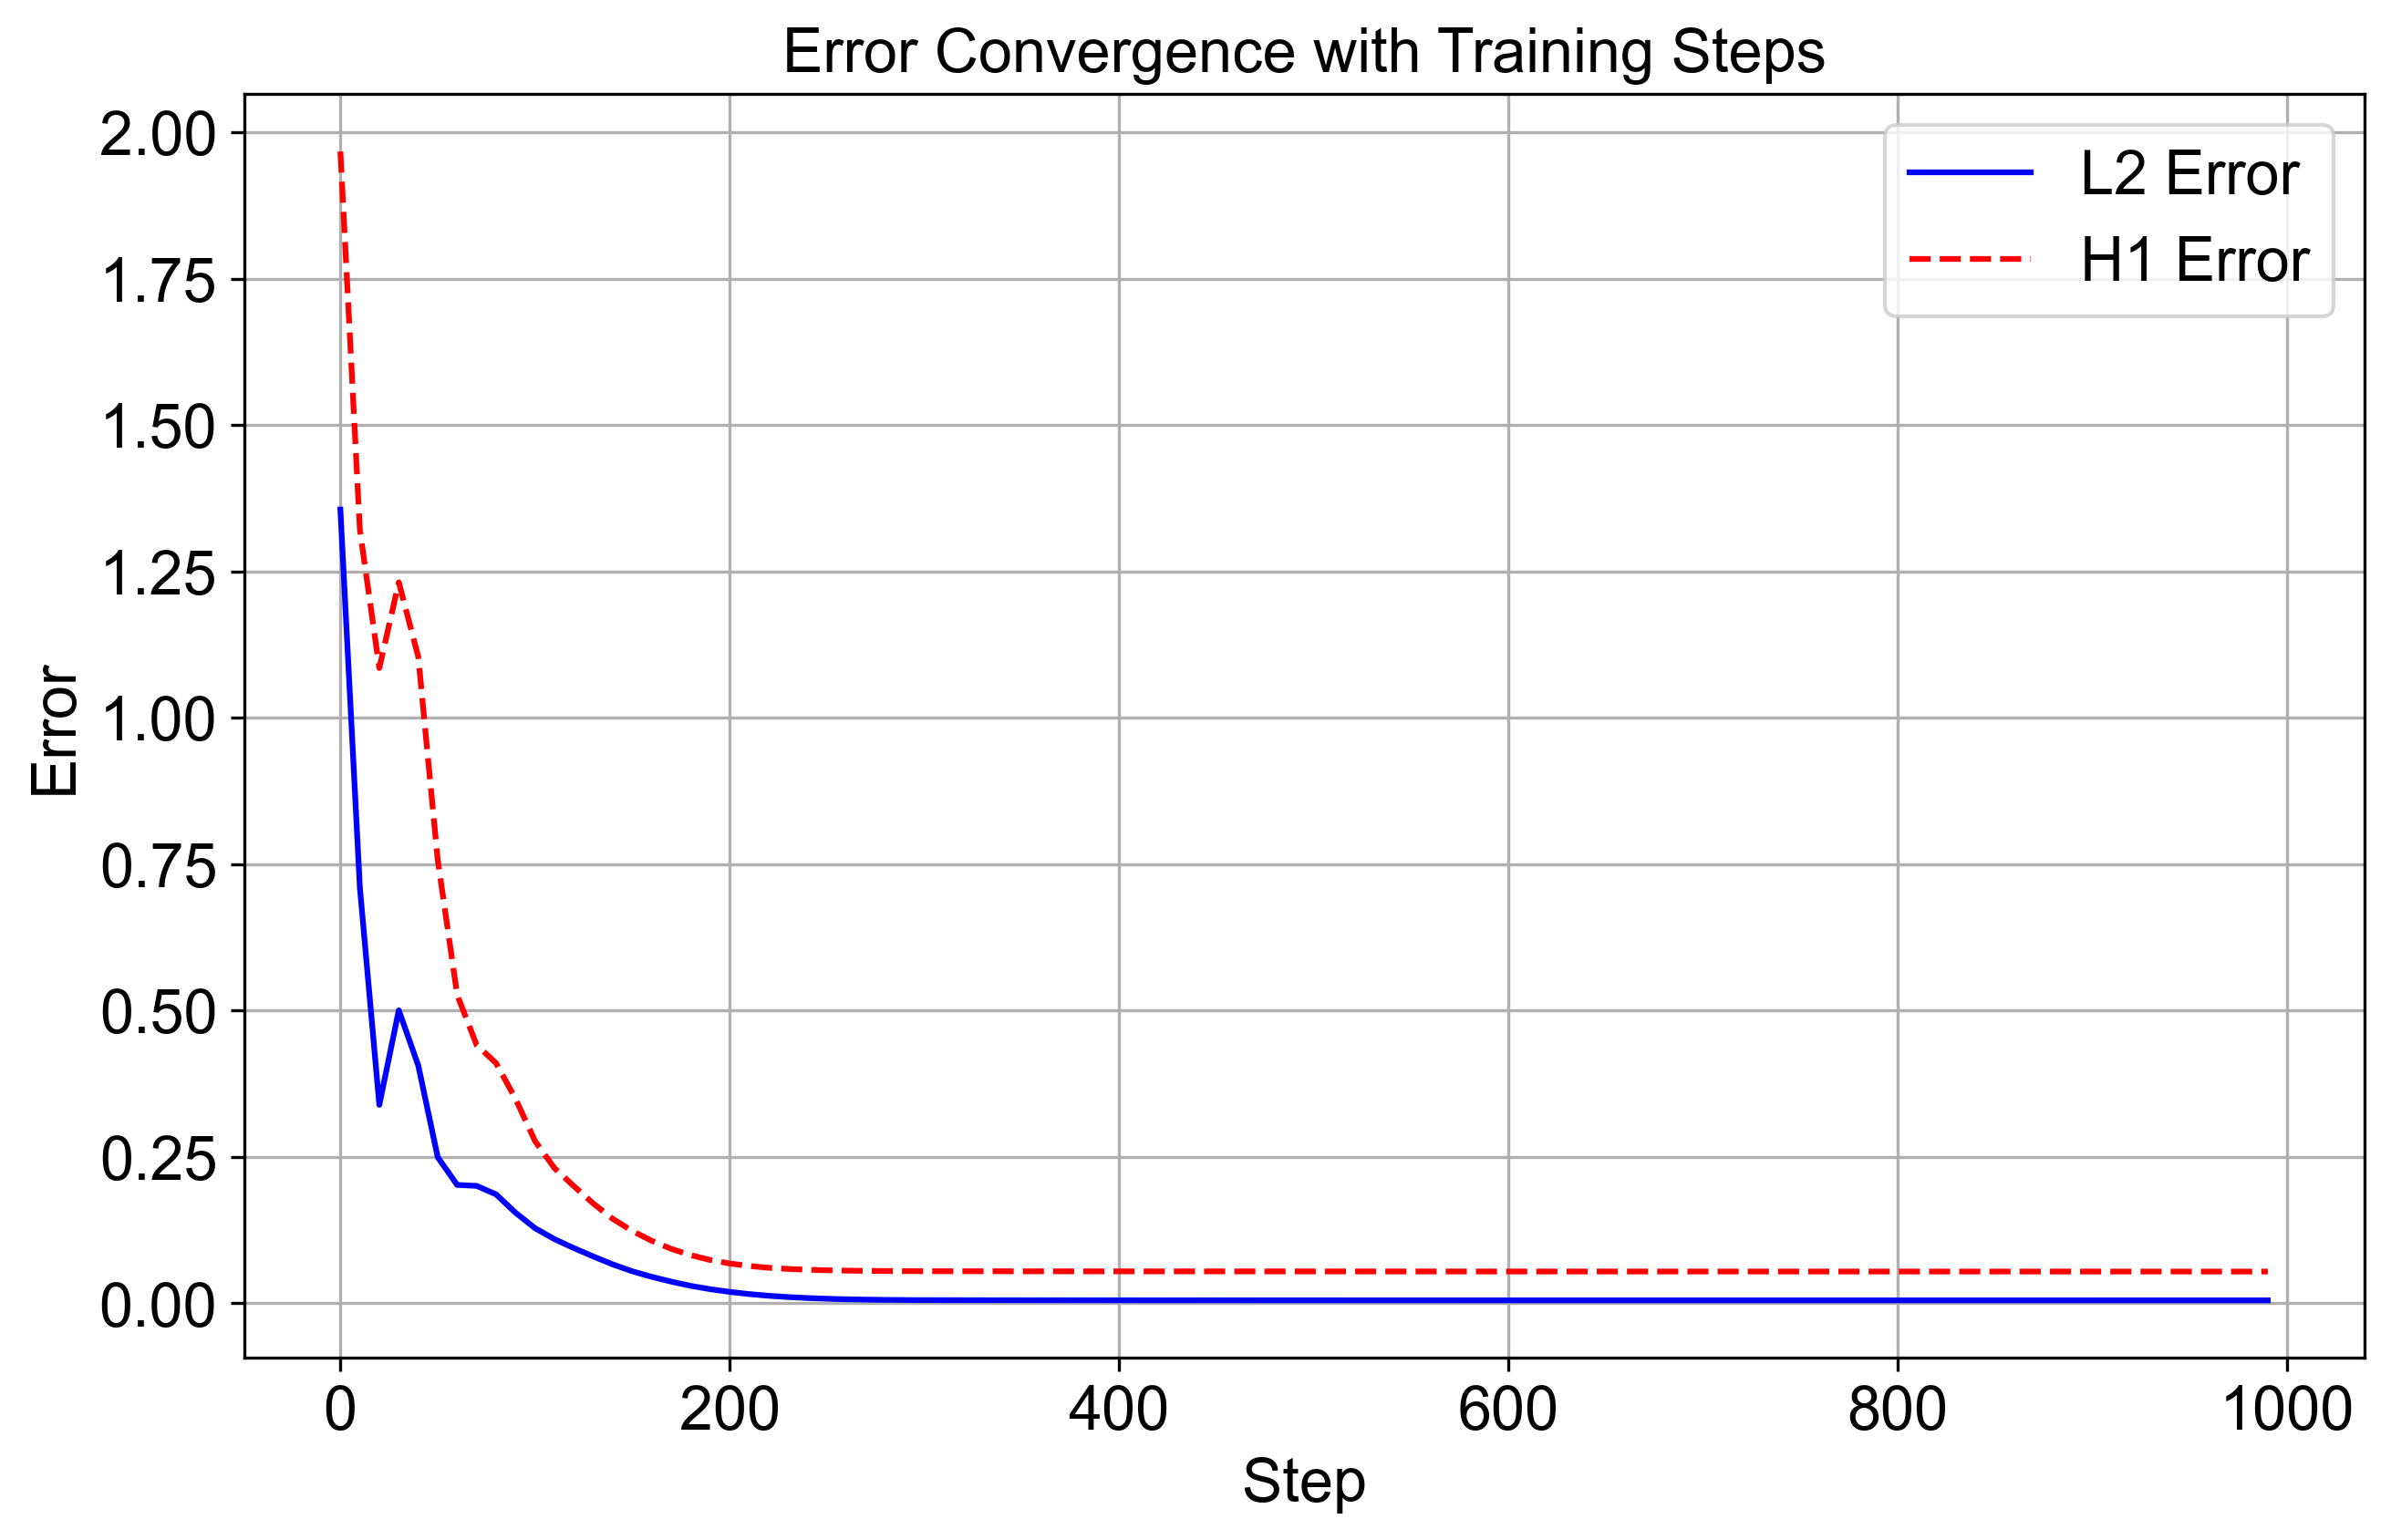
\includegraphics[width=\textwidth, height=6cm, keepaspectratio]{figures/5-1-6.png}
        \caption{再生核增强1000步误差收敛曲线}
        \label{fig:absolute_error}
    \end{subfigure}
   
    \centering
    \caption{1000步误差收敛可视化}
    \label{fig:combined}
\end{figure}

Deep里兹 方法初始 L2 误差和 H1 误差较高（2.0 和 1.75），前 200 步下降至 0.5 和 0.75，最终稳定在 0.25 和 0.5，但存在波动且导数拟合较弱；RK-Deep里兹 方法初始误差较低（1.4-1.6），收敛更快，最终误差降至 0.1 和 0.2，训练更稳定，H1 误差与 L2 误差差距较小，显示出再生核增强对函数值和导数拟合的显著改进。

\begin{figure}[htbp]
    \centering
    \begin{subfigure}[b]{0.45\textwidth}
        \centering
        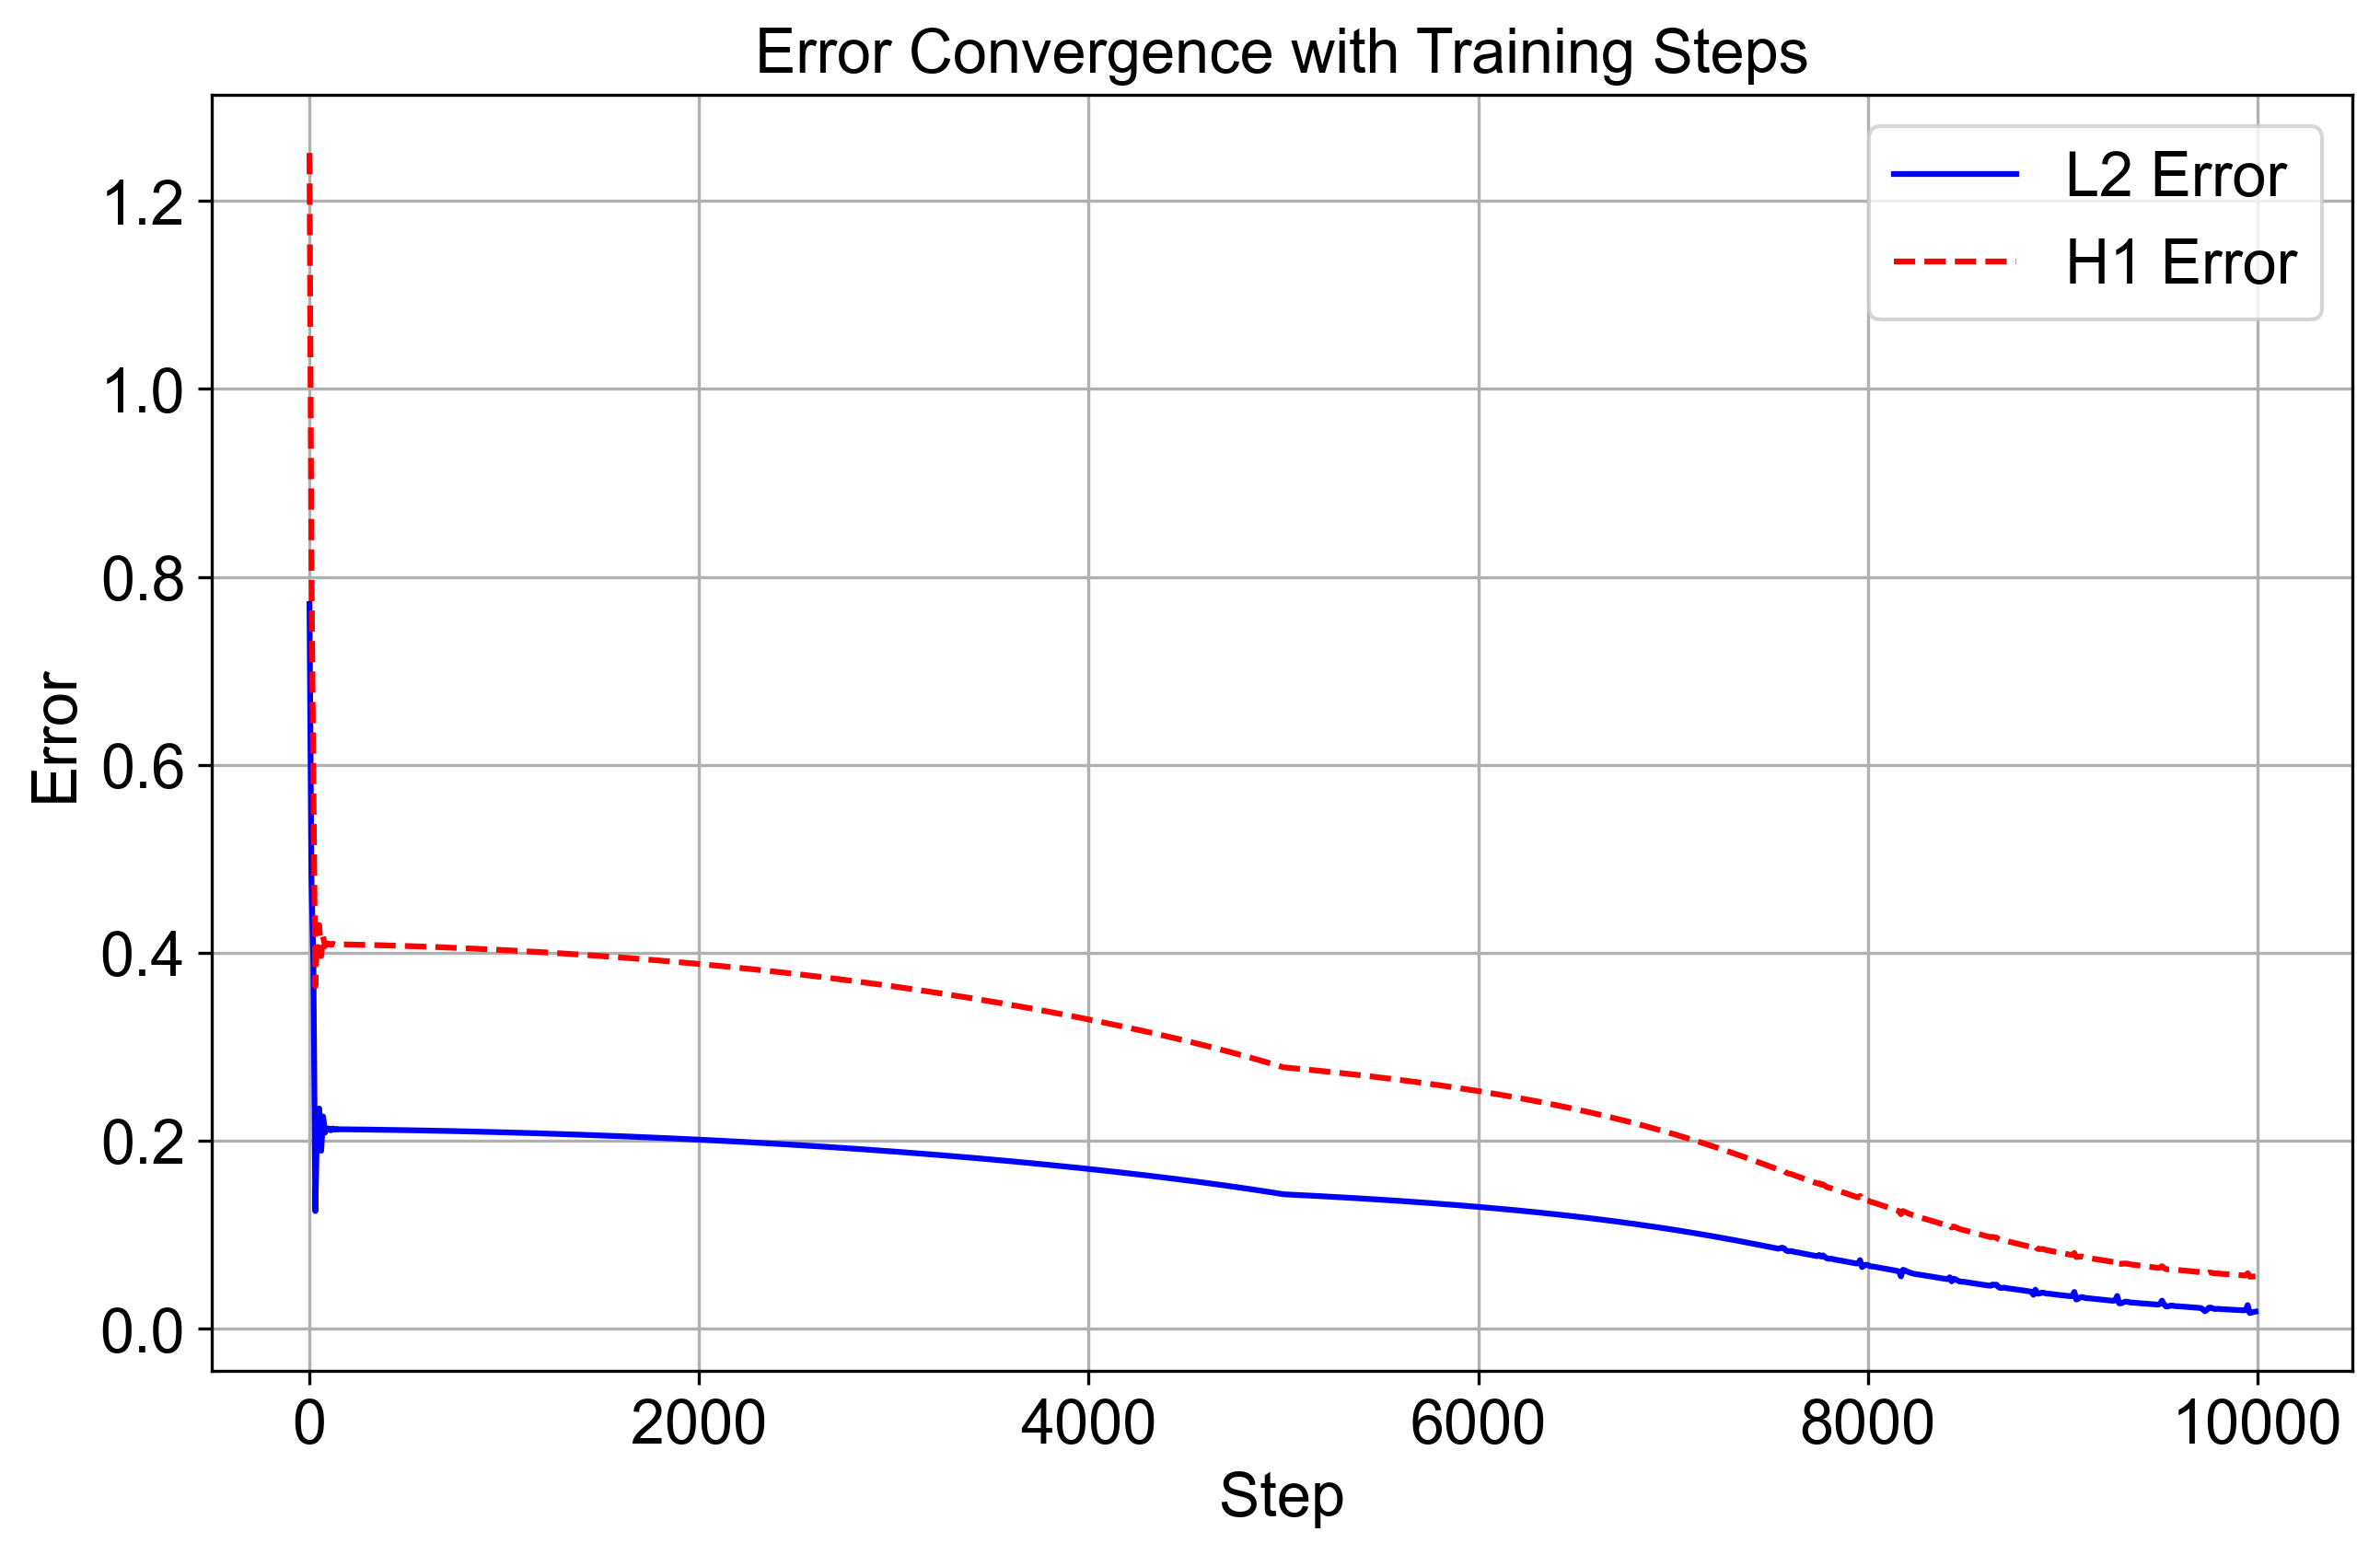
\includegraphics[width=\textwidth, height=6cm, keepaspectratio]{figures/3-2-6.png}
        \caption{深度里兹法10000步误差收敛曲线}
        \label{fig:deepritz_solutions}
    \end{subfigure}
    \hfill
    \begin{subfigure}[b]{0.45\textwidth}
        \centering
        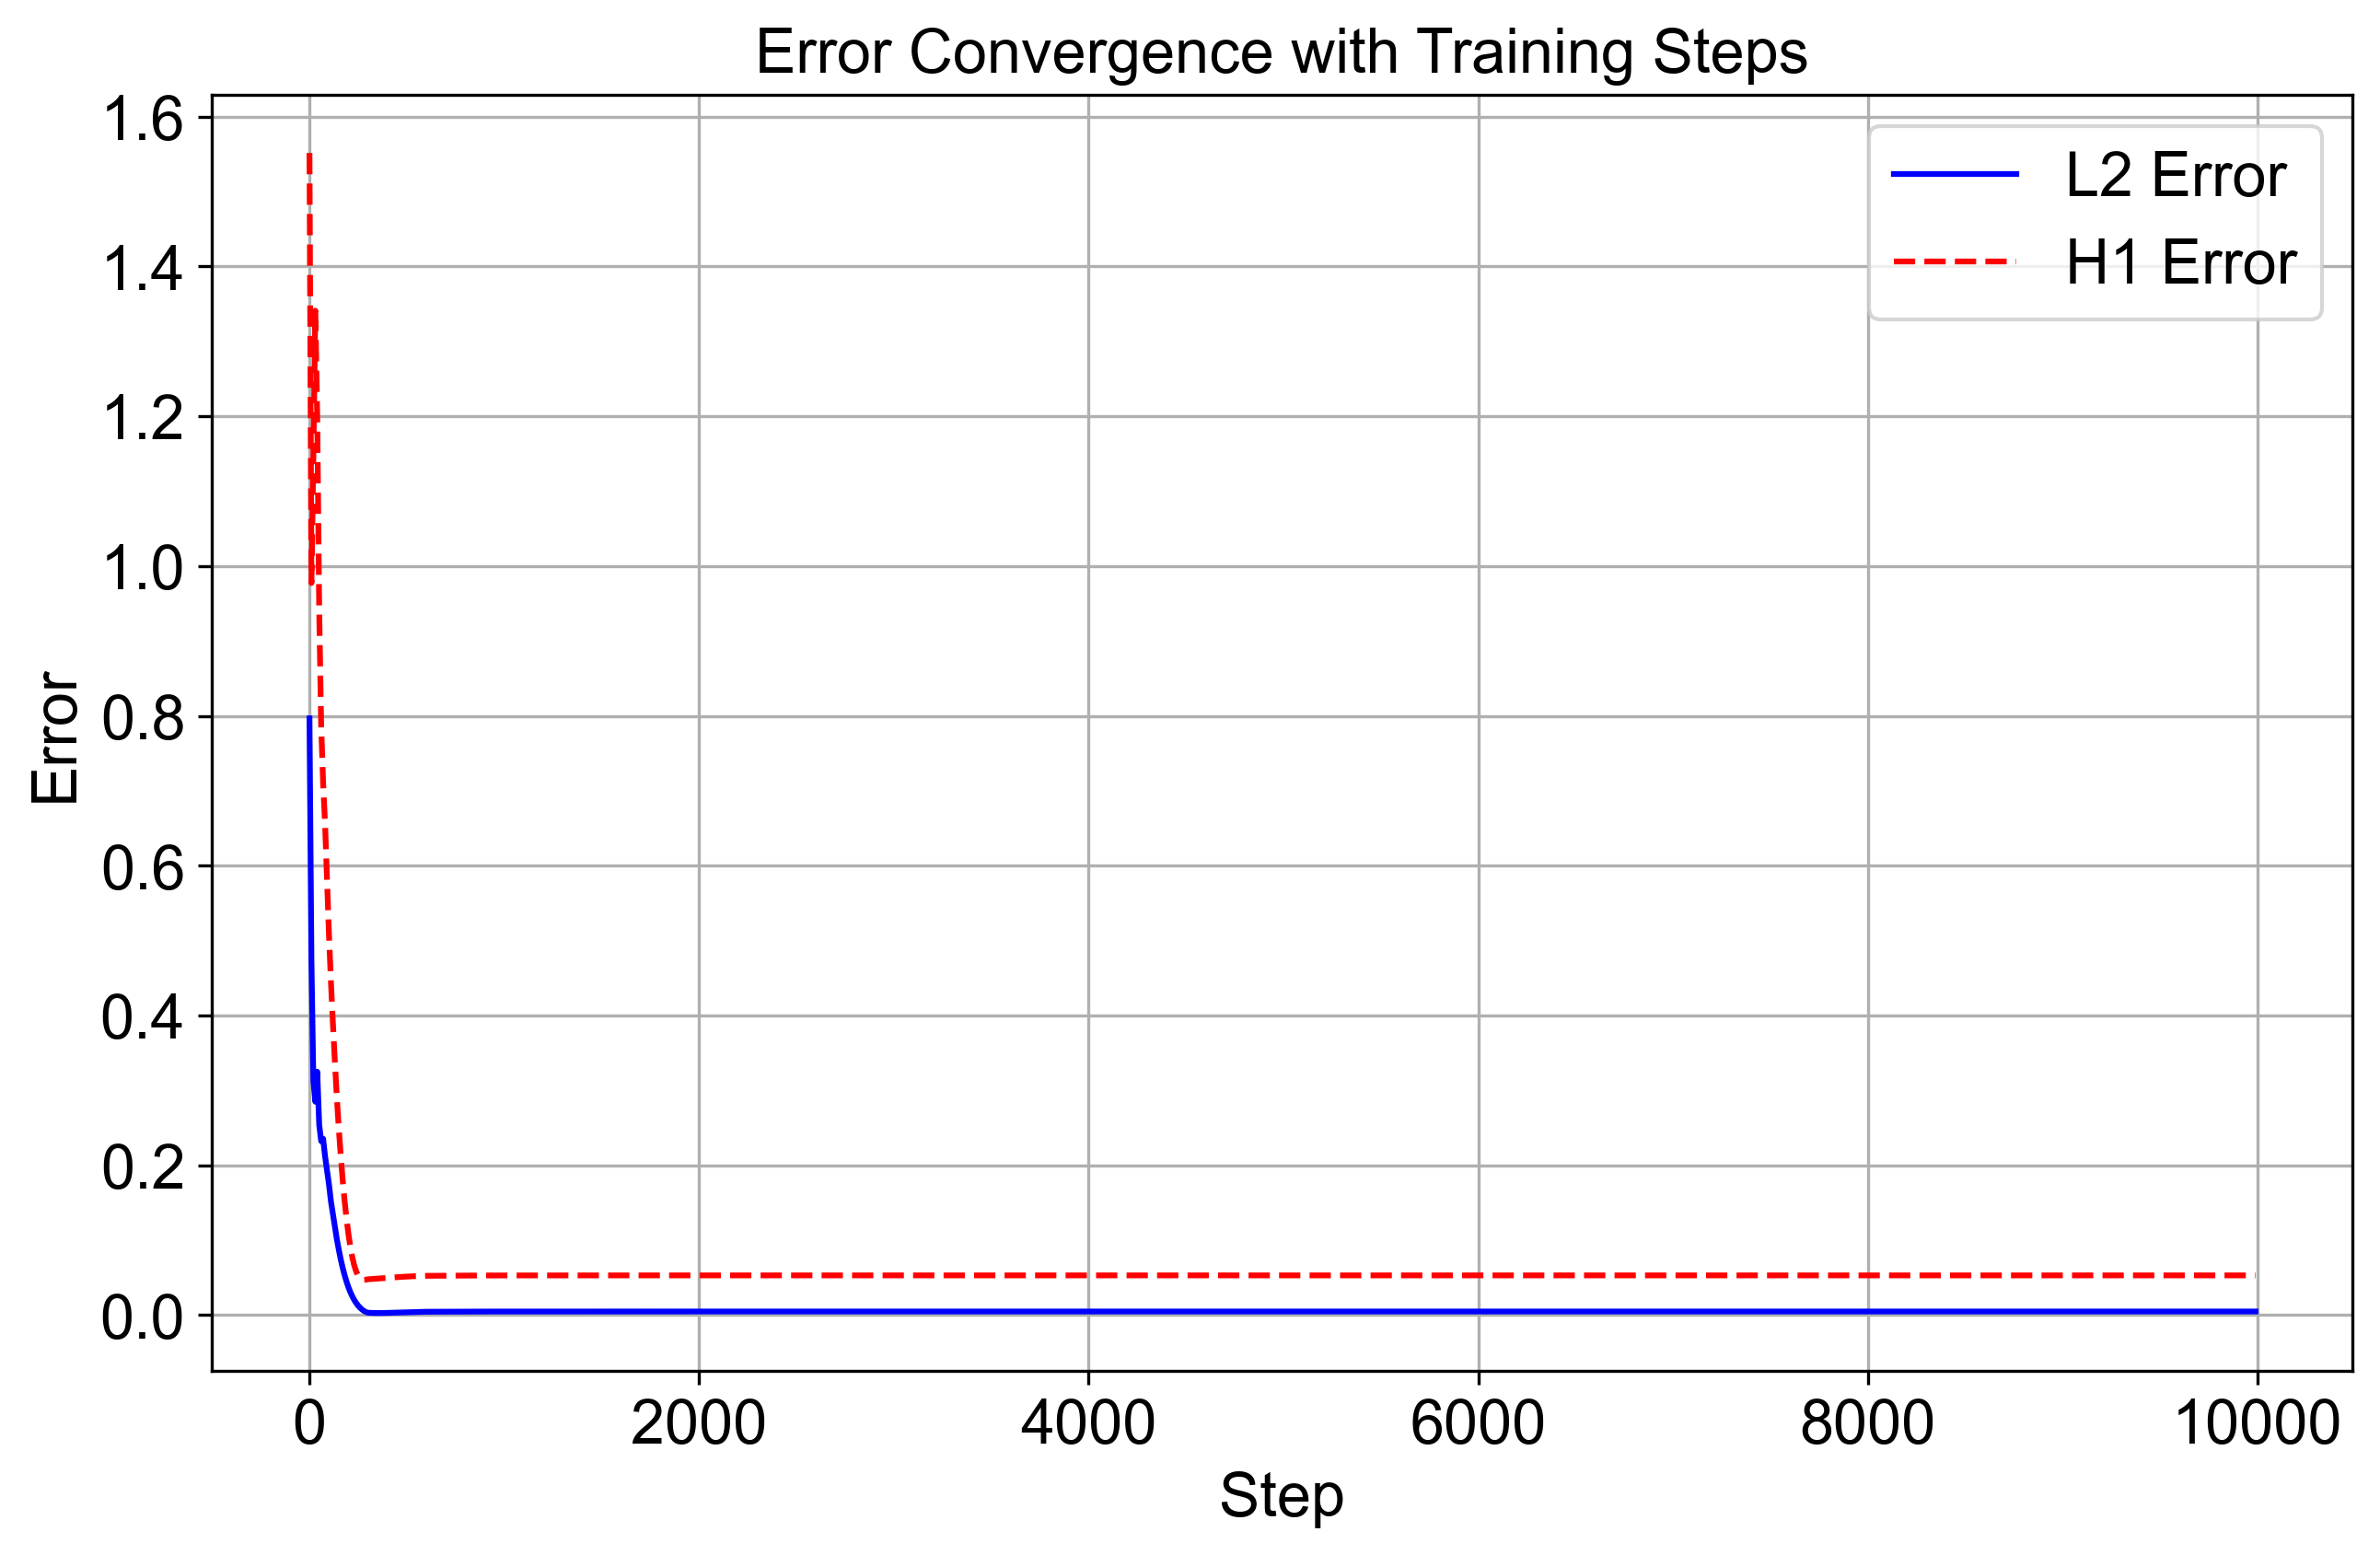
\includegraphics[width=\textwidth, height=6cm, keepaspectratio]{figures/5-2-6.png}
        \caption{再生核增强10000步误差收敛曲线}
        \label{fig:absolute_error}
    \end{subfigure}
   
    \centering
    \caption{10000步误差收敛可视化}
    \label{fig:combined}
\end{figure}
Deep里兹 方法经训练后误差显著降低，但导数拟合仍为瓶颈。RK-Deep里兹 方法收敛更快，精度更高。
\subsection{计算时间对比}
\begin{figure}[ht]
    \centering
    \begin{minipage}{0.48\textwidth}
        \centering
        \begin{tikzpicture}
        \begin{axis}[
            title={训练时间对比},
            ybar,
            bar width=0.2cm,
            enlargelimits=0.2,
            legend style={at={(0.5,-0.2)}, anchor=north, legend columns=-1},
            ylabel={训练时间 (秒)},
            symbolic x coords={1000 步, 10000 步, 20000 步},
            xtick=data,
            ymin=0, ymax=300,
            nodes near coords,
            nodes near coords align={vertical},
            every node near coord/.append style={font=\scriptsize, xshift=0pt, yshift=2pt},
            width=\textwidth,
            height=6cm
        ]
        \addplot[fill=blue!50] coordinates {(1000 步, 3.36) (10000 步, 34.79) };
        \addplot[fill=green!50] coordinates {(1000 步, 23.95) (10000 步, 244.76) }; % 添加 20000 步数据，假设为 0
        \legend{Deep里兹 方法, RK-Deep里兹 方法}
        \end{axis}
        \end{tikzpicture}
    \end{minipage}
    \hfill
    \begin{minipage}{0.48\textwidth}
        \centering
        \begin{tikzpicture}
        \begin{axis}[
            title={计算时间对比},
            ybar,
            bar width=0.2cm,
            enlargelimits=0.2,
            legend style={at={(0.5,-0.2)}, anchor=north, legend columns=-1},
            ylabel={计算时间 (秒)},
            symbolic x coords={1000 步, 10000 步, 伽辽金无网格},
            xtick=data,
            ymin=0, ymax=0.35,
            nodes near coords,
            nodes near coords align={vertical},
            every node near coord/.append style={font=\scriptsize, xshift=0pt, yshift=2pt},
            width=\textwidth,
            height=6cm
        ]
        \addplot[fill=blue!50] coordinates {(1000 步, 0.001) (10000 步, 0.0015)}; % Deep里兹 计算时间
        \addplot[fill=green!50] coordinates {(1000 步, 0.01) (10000 步, 0.01)}; % RK-Deep里兹 计算时间
        \addplot[fill=red!50] coordinates {(伽辽金无网格, 0.3)}; % 伽辽金无网格计算时间
        \legend{Deep里兹 方法, RK-Deep里兹 方法, 伽辽金无网格方法}
        \end{axis}
        \end{tikzpicture}
    \end{minipage}
    \caption{训练时间和计算时间对比}
    \label{fig:time_comparison}
\end{figure}
    
    从图 \ref{fig:time_comparison} 可以看出，Deep里兹 方法的训练时间随步数增加显著增长，而 RK-Deep里兹 方法训练时间更长，反映了再生核增强引入的额外计算开销。

\newpage
\subsection{对比RKPM方法}

\subsection*{训练精度对比}
\begin{figure}[htbp]
    \centering
    \begin{subfigure}[b]{0.45\textwidth}
        \centering
        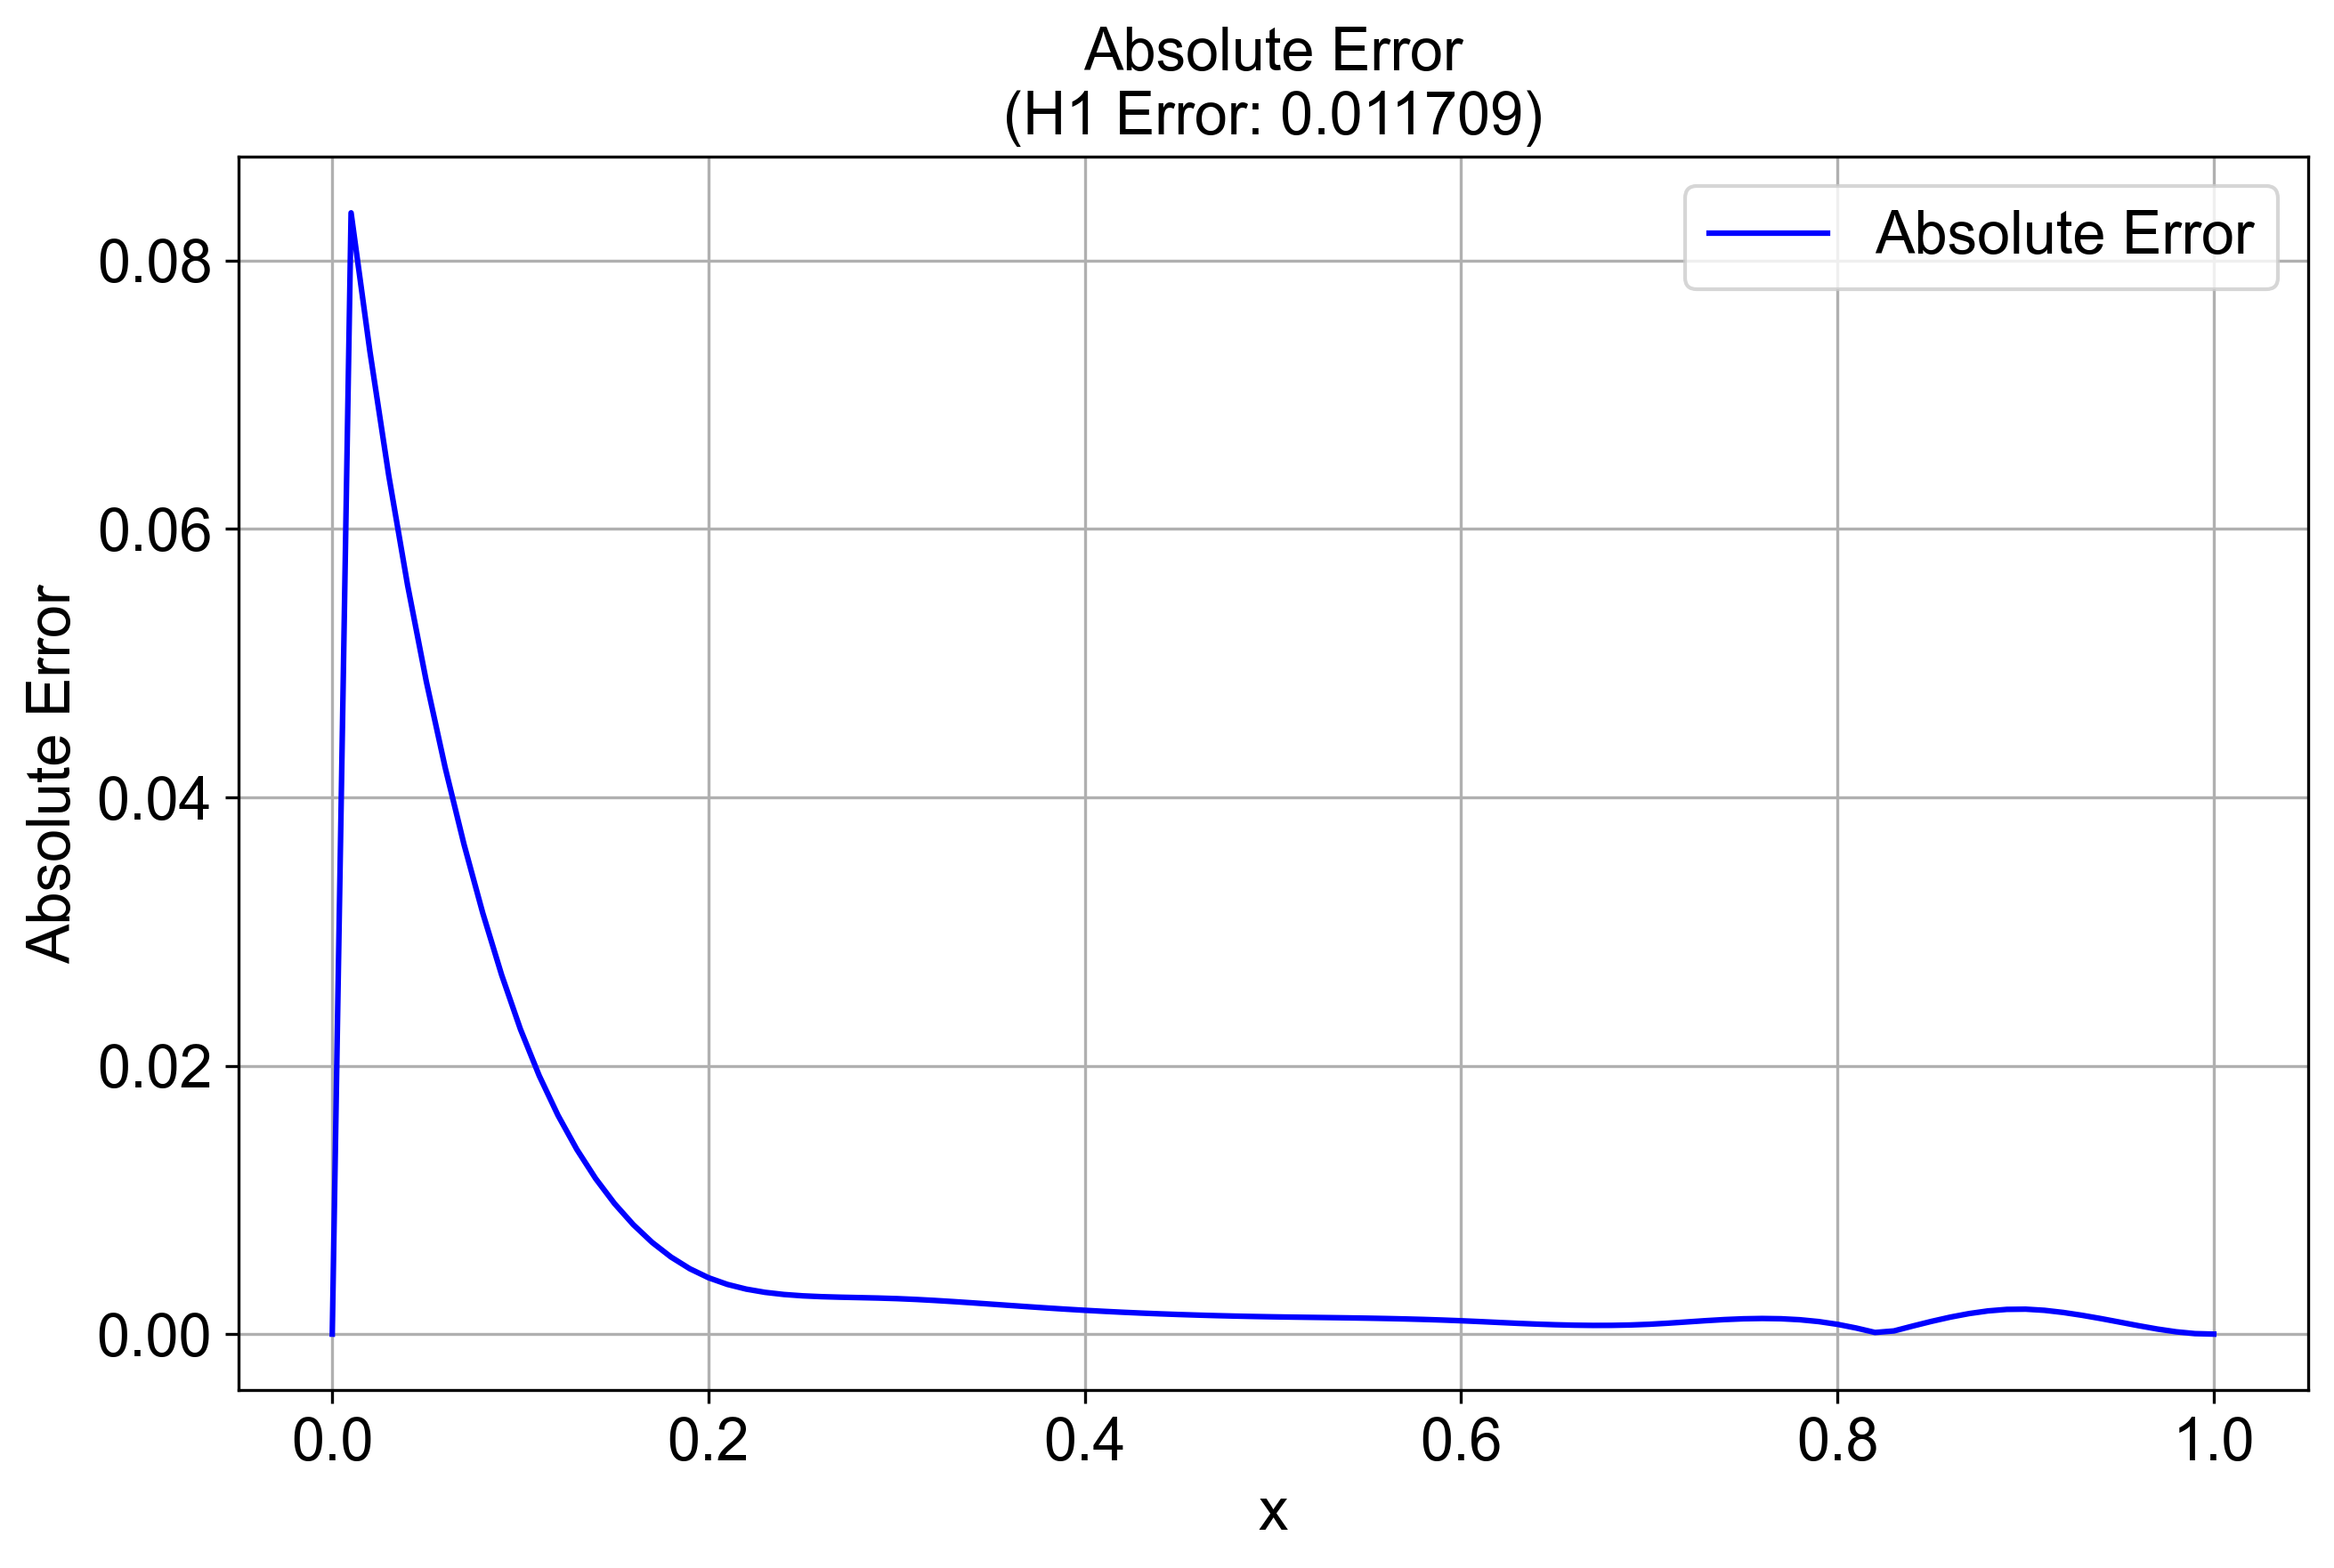
\includegraphics[width=\textwidth, height=6cm, keepaspectratio]{figures/4-2.png}
        \caption{RKPM方法绝对误差}
        \label{fig:deepritz_solutions}
    \end{subfigure}
    \hfill
    \begin{subfigure}[b]{0.45\textwidth}
        \centering
        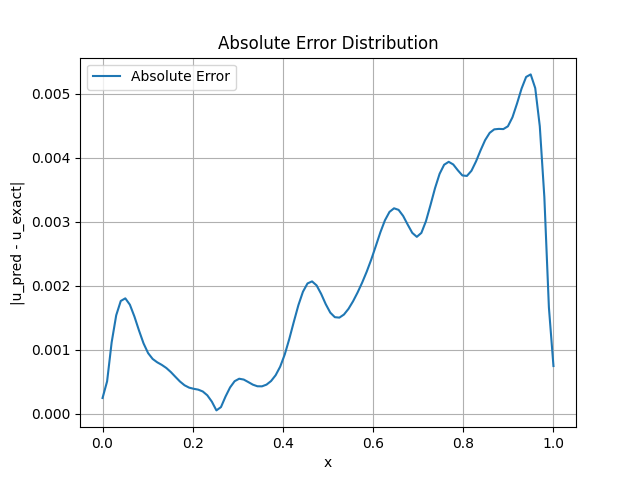
\includegraphics[width=\textwidth, height=6cm, keepaspectratio]{figures/5-1-2.png}
        \caption{再生核增强10000步绝对误差}
        \label{fig:absolute_error}
    \end{subfigure}

    \centering
    \caption{误差可视化。}
    \label{fig:combined}
\end{figure}

\begin{figure}[htbp]
    \centering
    \begin{subfigure}[b]{0.45\textwidth}
        \centering
        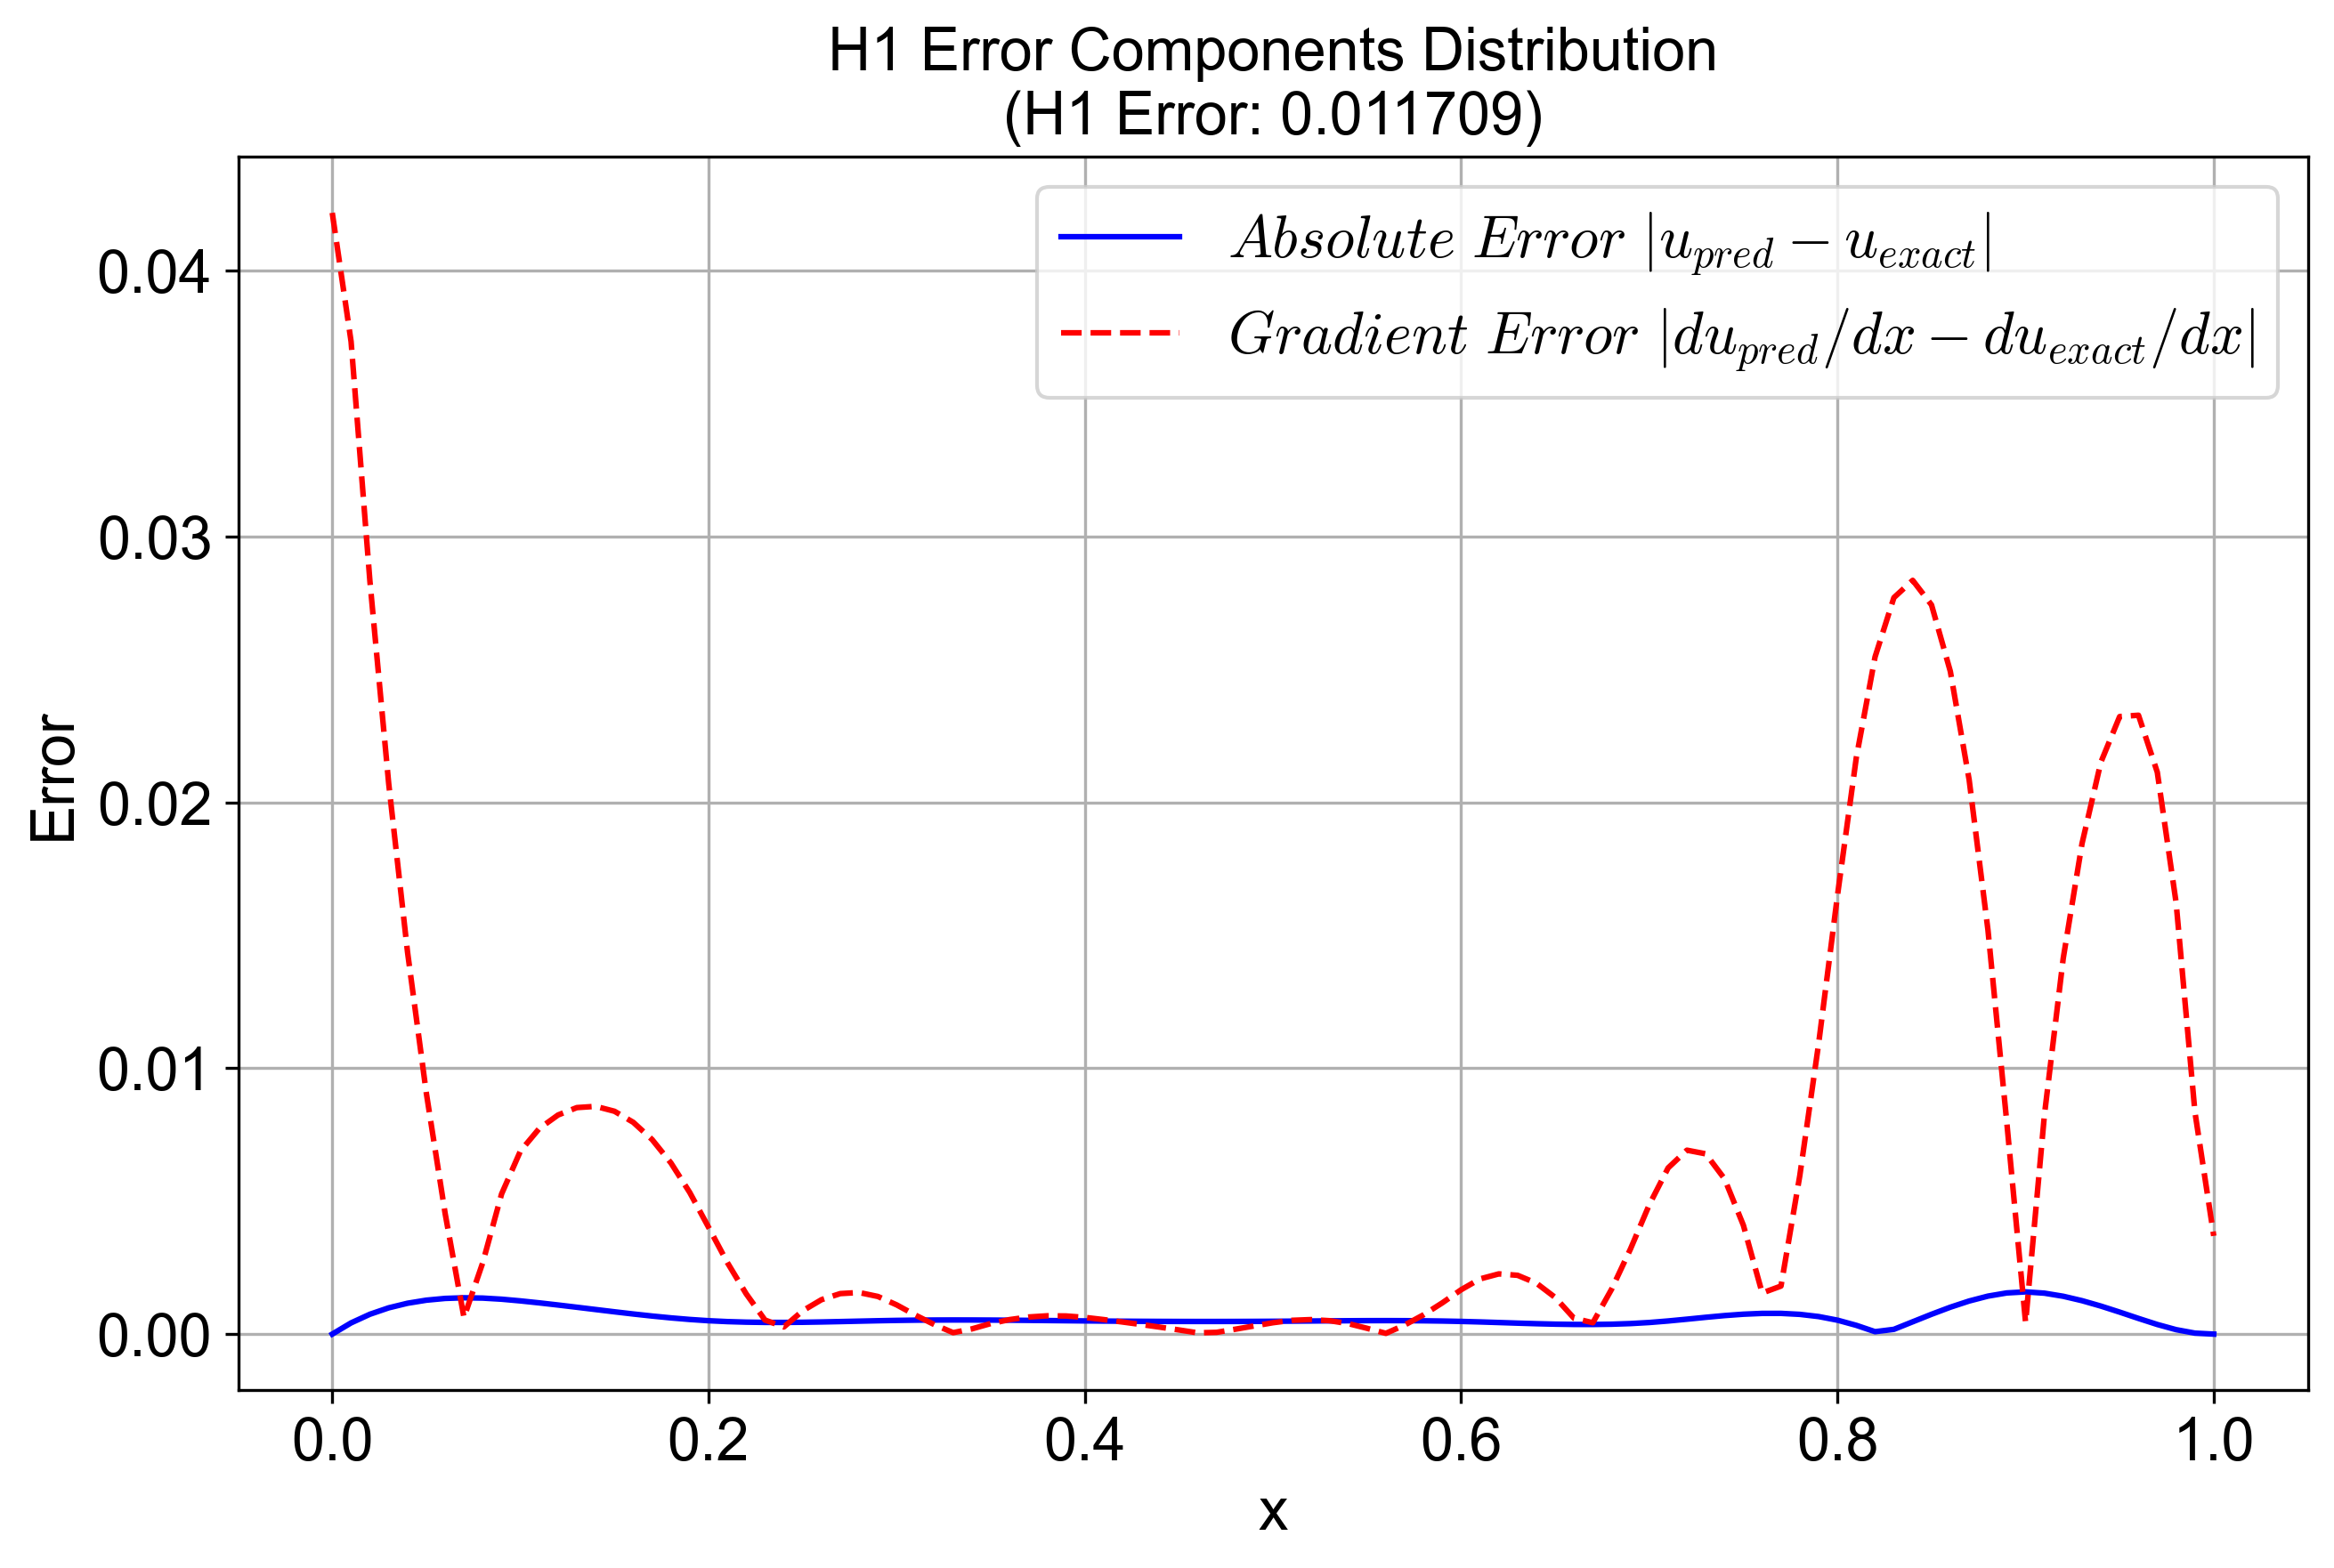
\includegraphics[width=\textwidth, height=6cm, keepaspectratio]{figures/4-3.png}
        \caption{RKPM方法L2误差}
        \label{fig:deepritz_solutions}
    \end{subfigure}
    \hfill
    \begin{subfigure}[b]{0.45\textwidth}
        \centering
        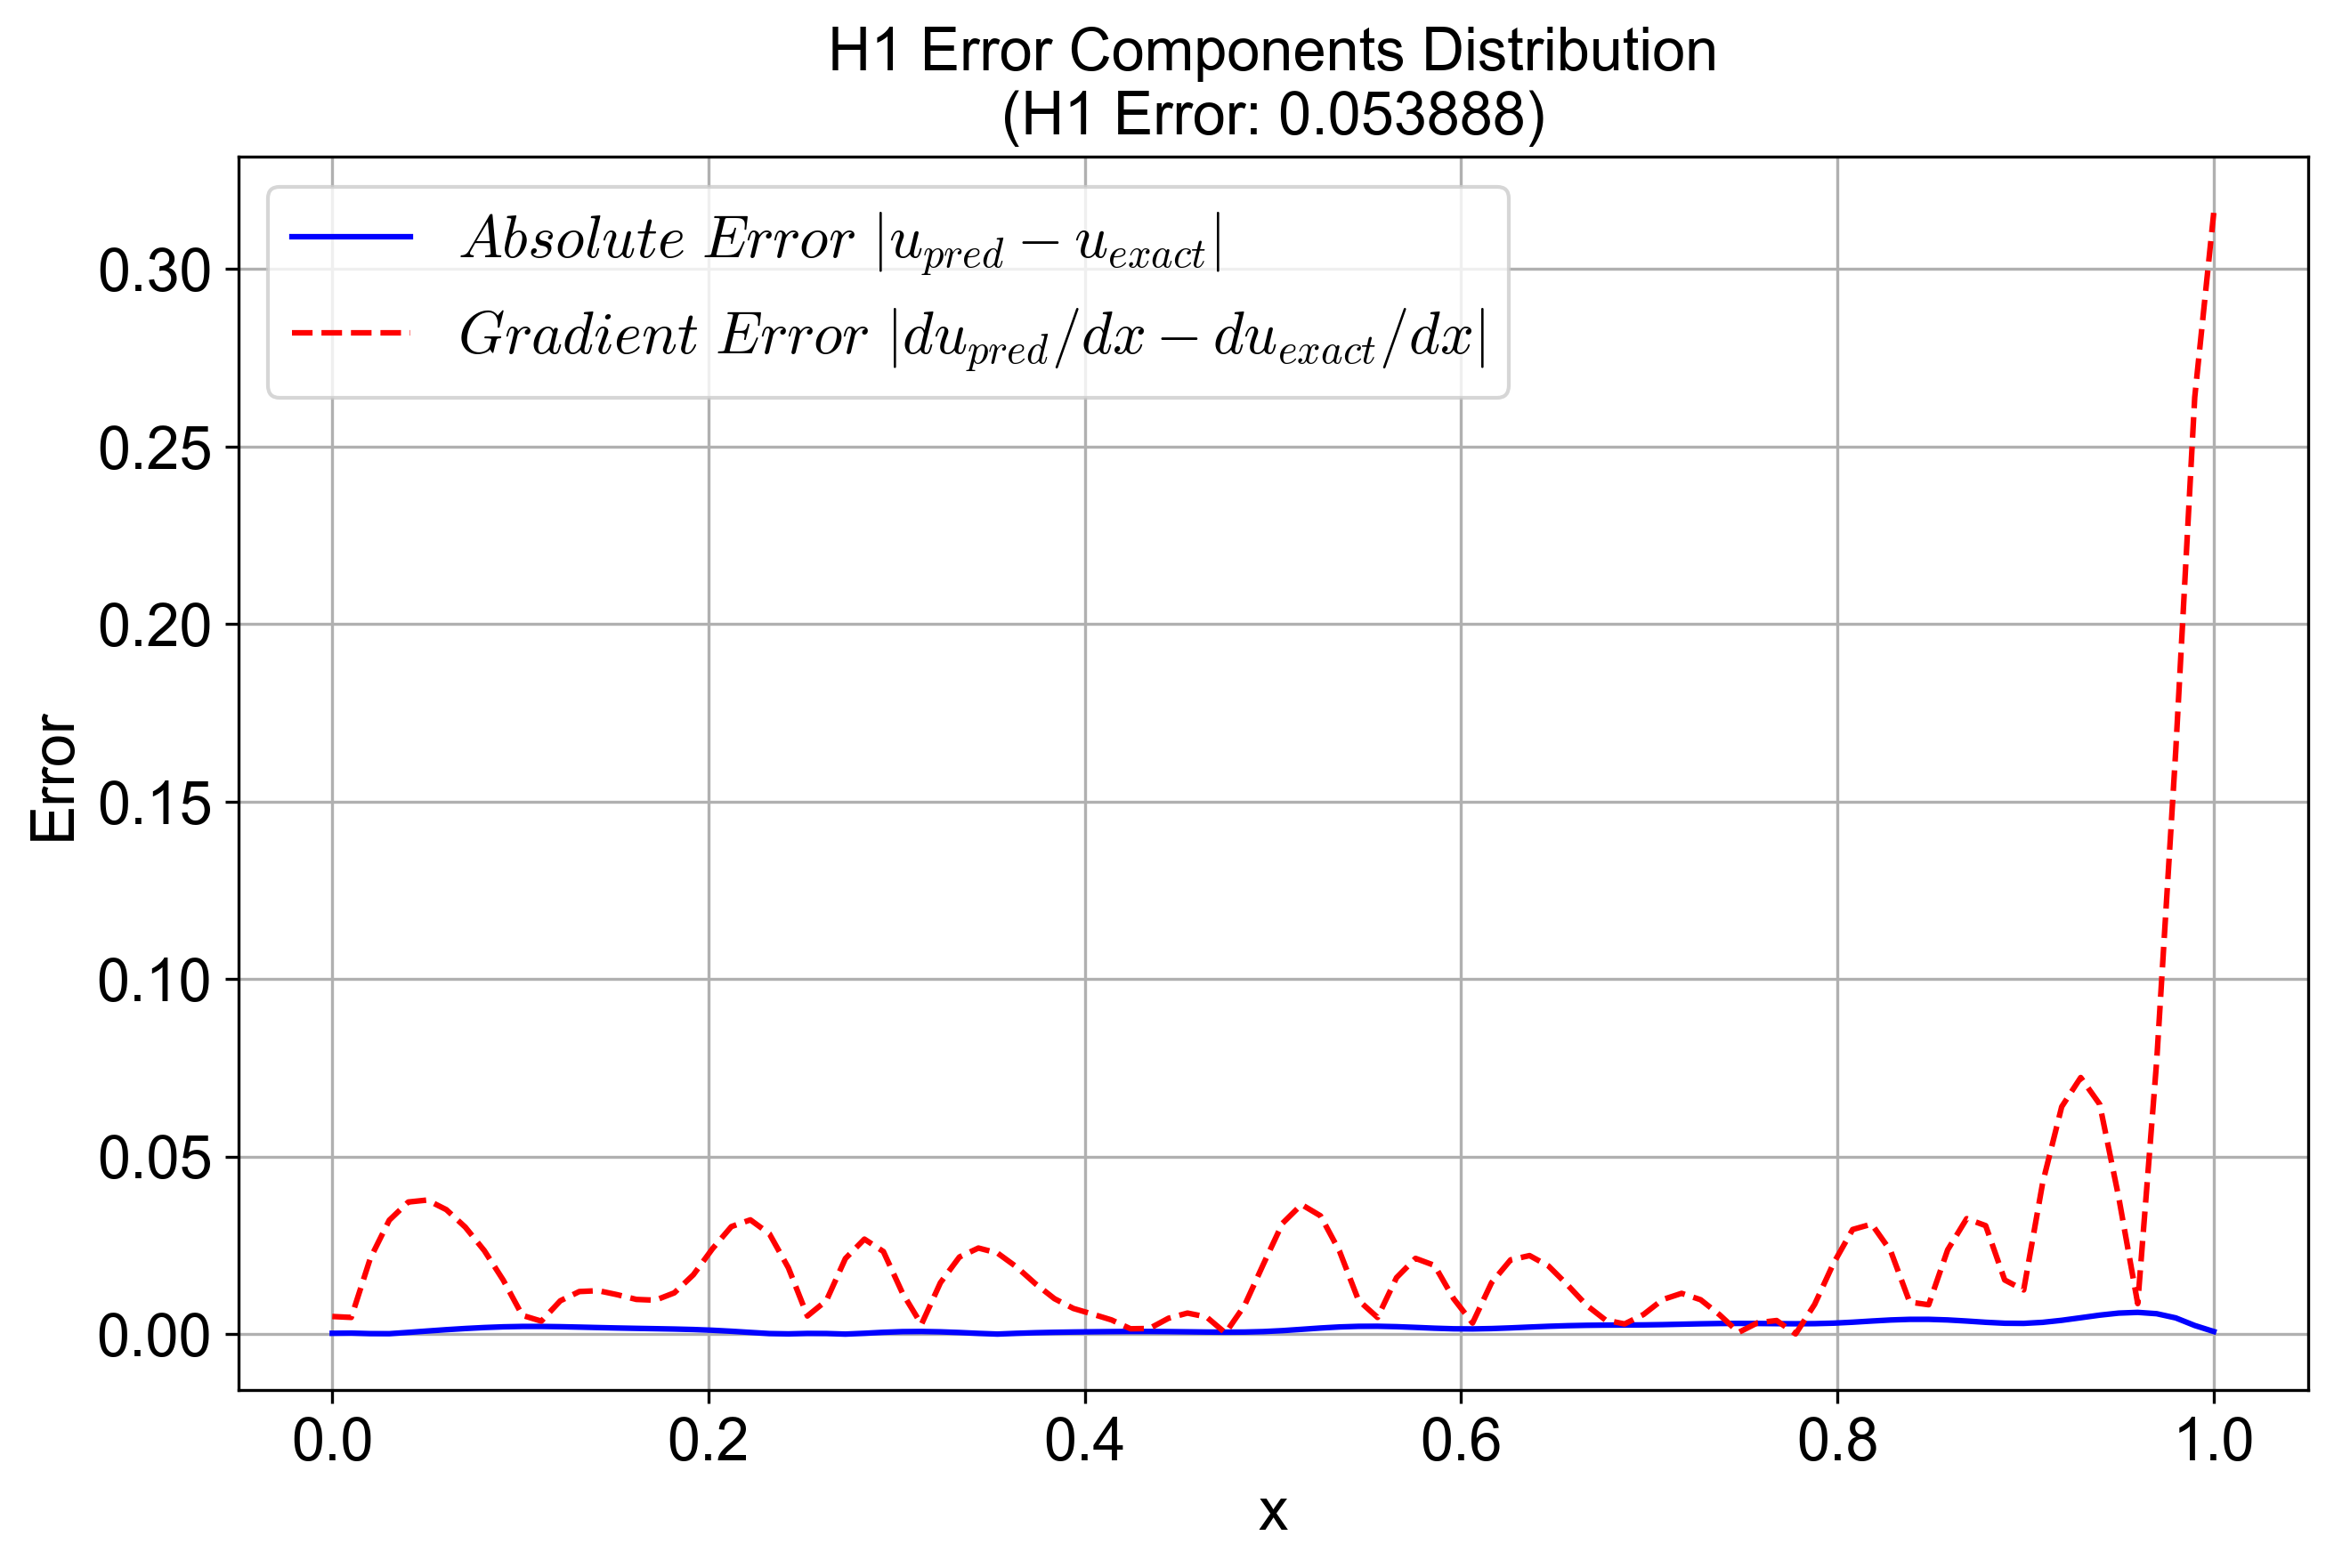
\includegraphics[width=\textwidth, height=6cm, keepaspectratio]{figures/5-1-5.png}
        \caption{再生核增强10000步L2误差}
        \label{fig:absolute_error}
    \end{subfigure}

    \centering
    \caption{L2误差对比}
    \label{fig:combined}
\end{figure}
RKPM 方法的误差分布平滑但边界处导数误差较大；RK-Deep里兹 方法的误差分布波动较大但精度更高，导数误差波动性强。RK-Deep里兹 结合深度学习显著提升了 L2 误差的拟合能力，但导数拟合较弱.


\subsection{小结}
\begin{figure}[htbp]
    \centering
    \begin{subfigure}[b]{0.45\textwidth}
        \centering
        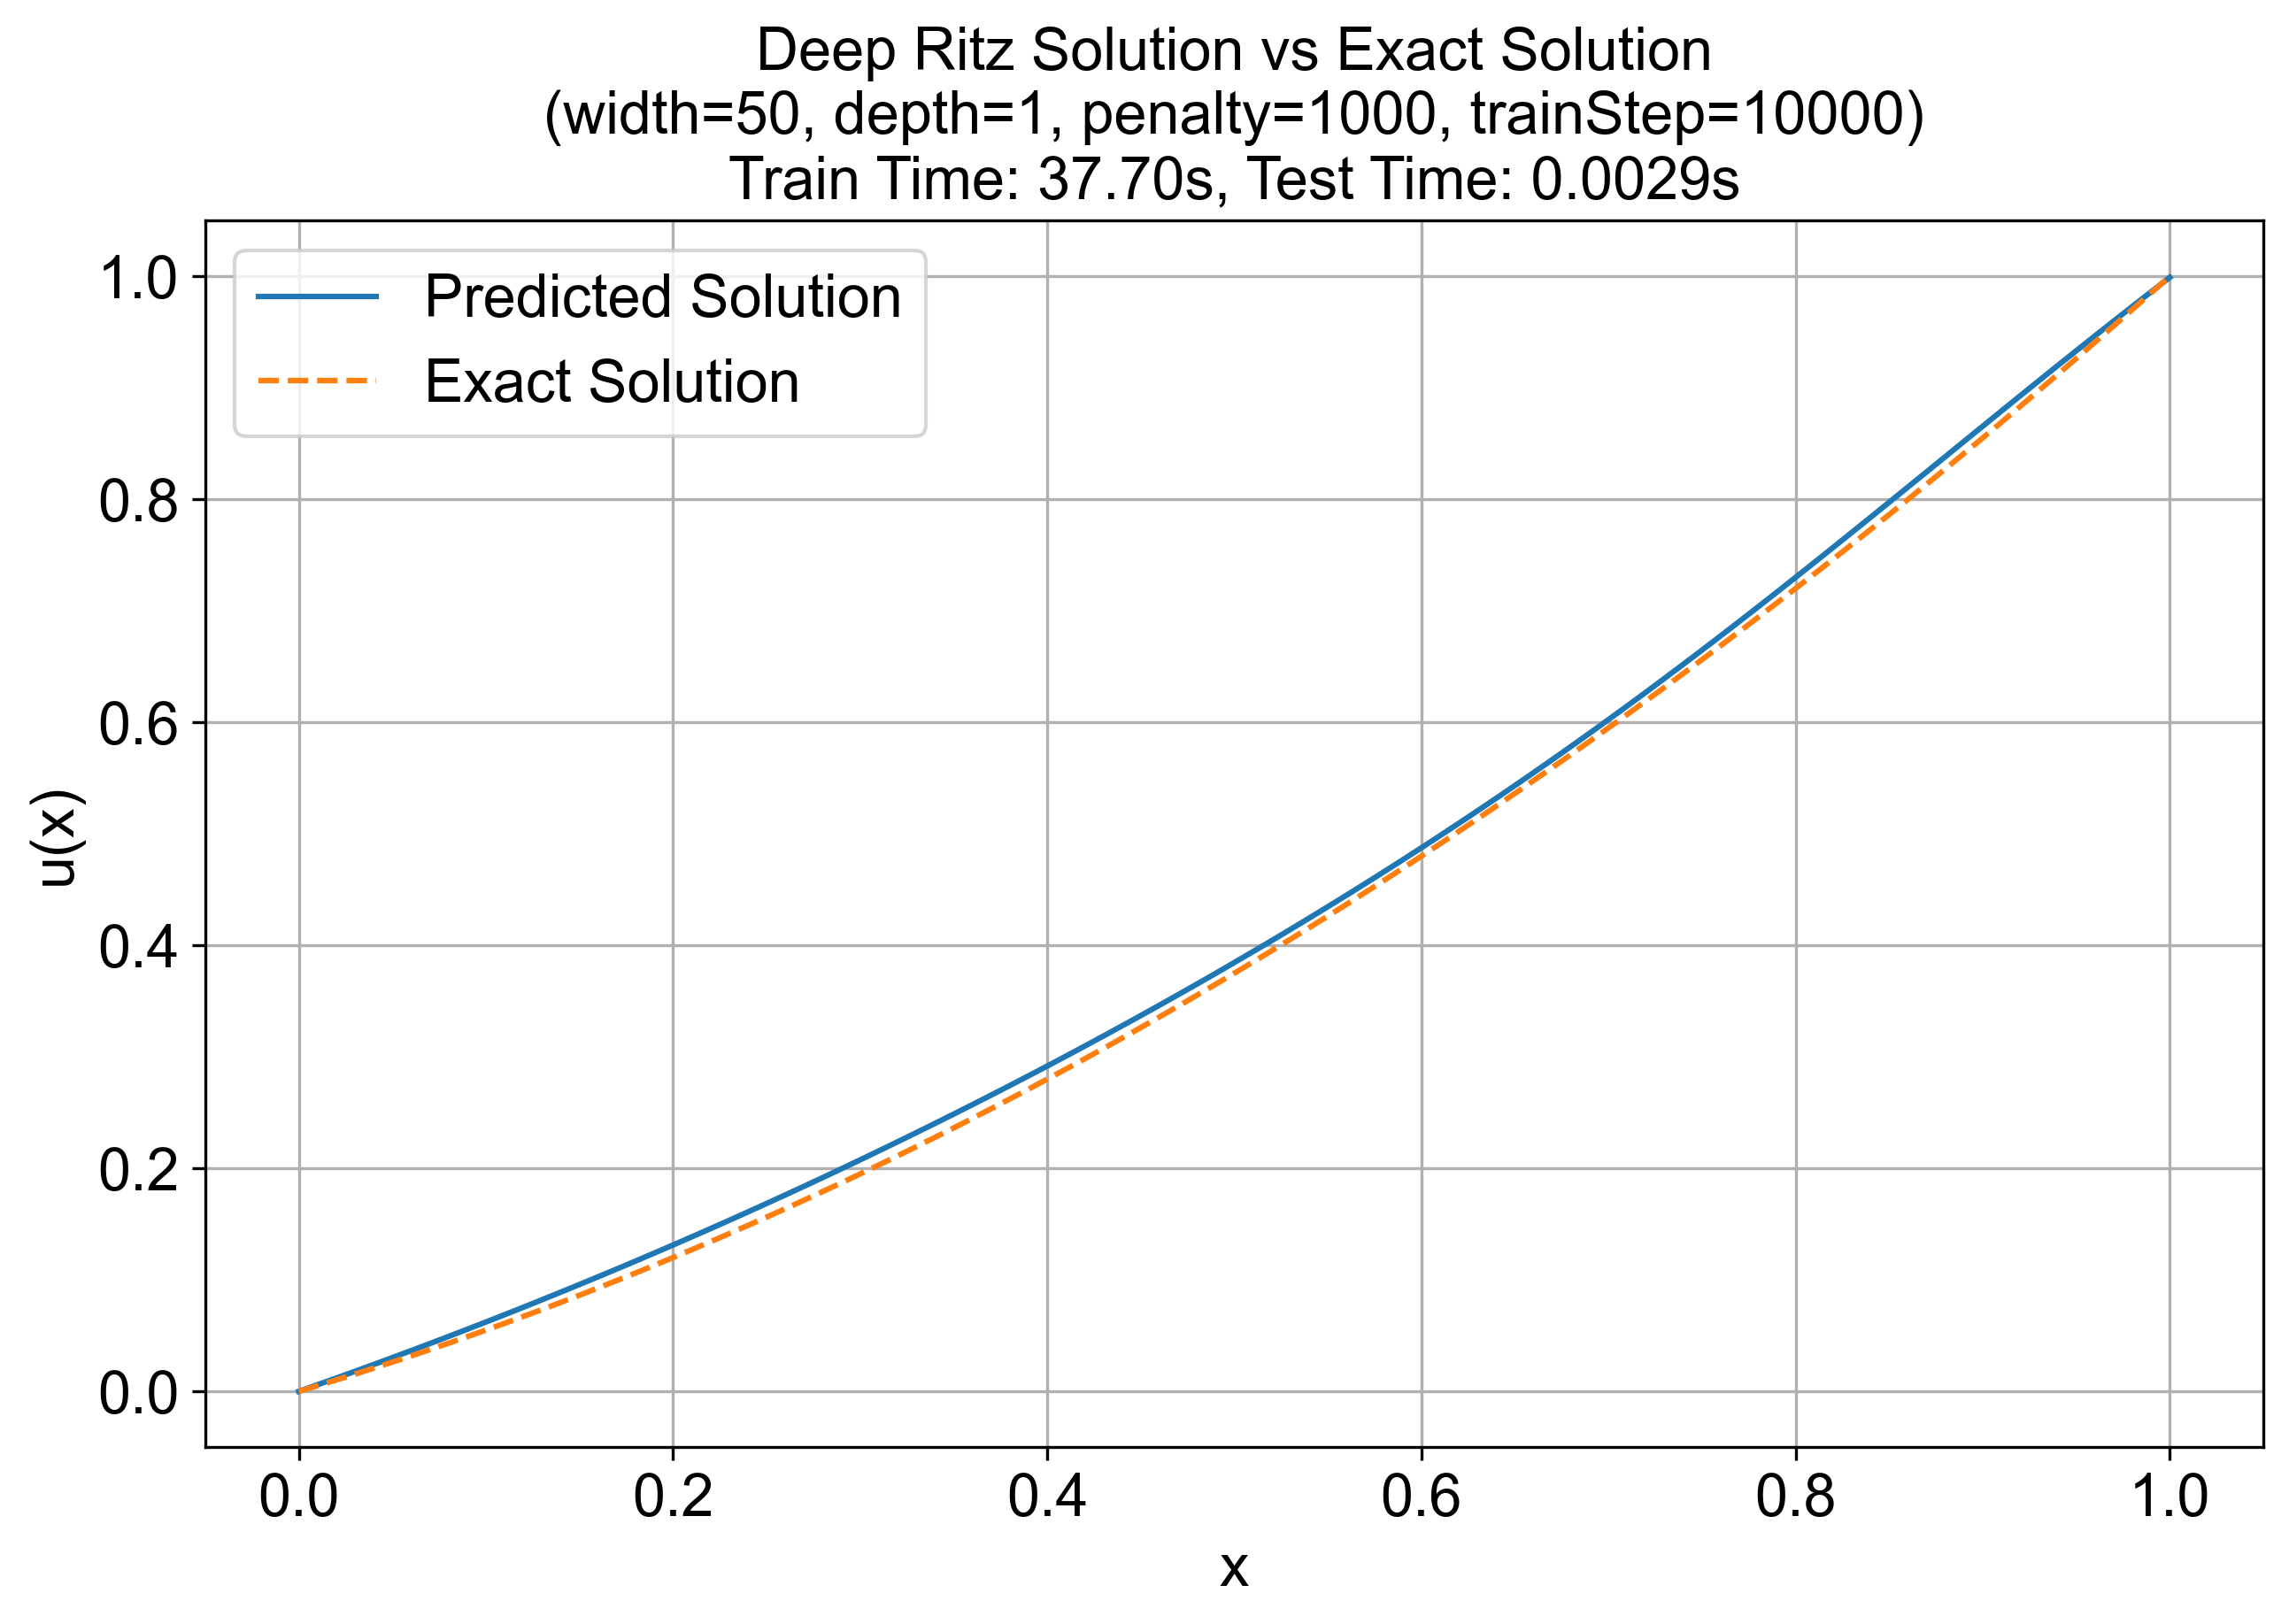
\includegraphics[width=\textwidth, height=6cm, keepaspectratio]{figures/3-2-1.png}
        \caption{RKPM方法绝对误差}
        \label{fig:deepritz_solutions}
    \end{subfigure}
    \hfill
    \begin{subfigure}[b]{0.45\textwidth}
        \centering
        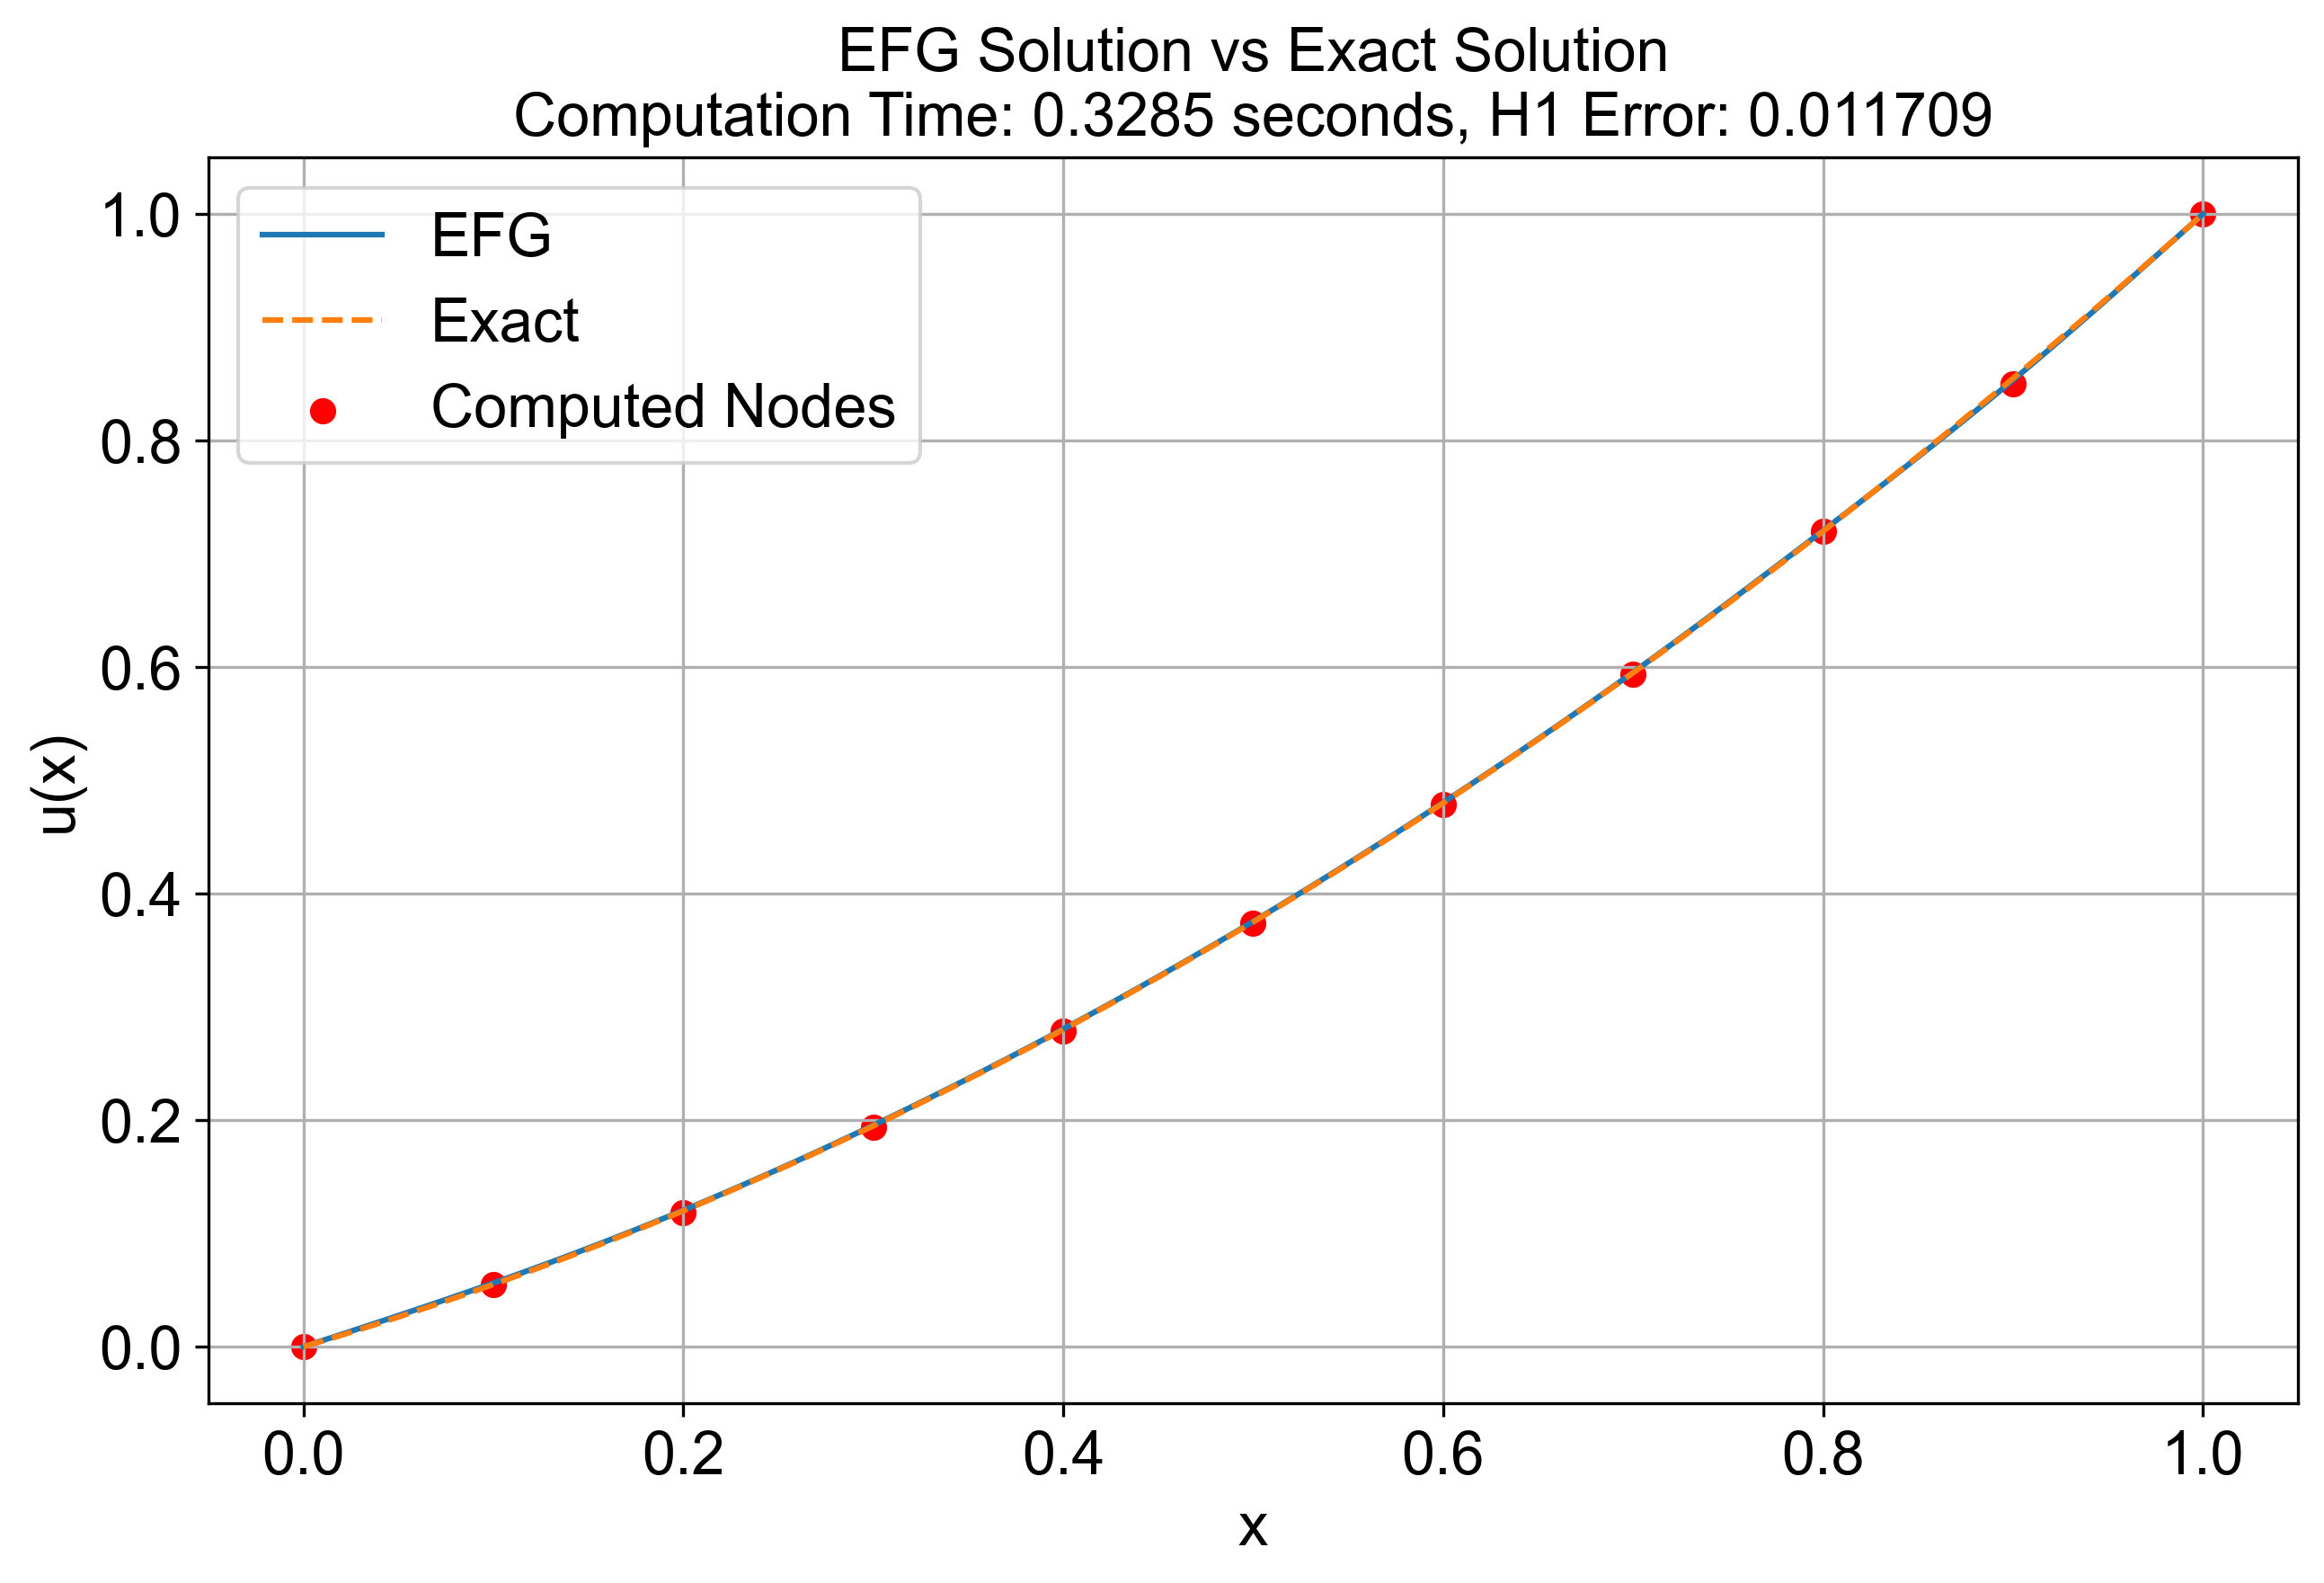
\includegraphics[width=\textwidth, height=6cm, keepaspectratio]{figures/4-1.png}
        \caption{再生核增强10000步绝对误差}
        \label{fig:absolute_error}
    \end{subfigure}

    \centering
    \caption{误差可视化。}
    \label{fig:combined}
\end{figure}

\begin{figure}[htbp]
    \centering
    \begin{subfigure}[b]{0.45\textwidth}
        \centering
        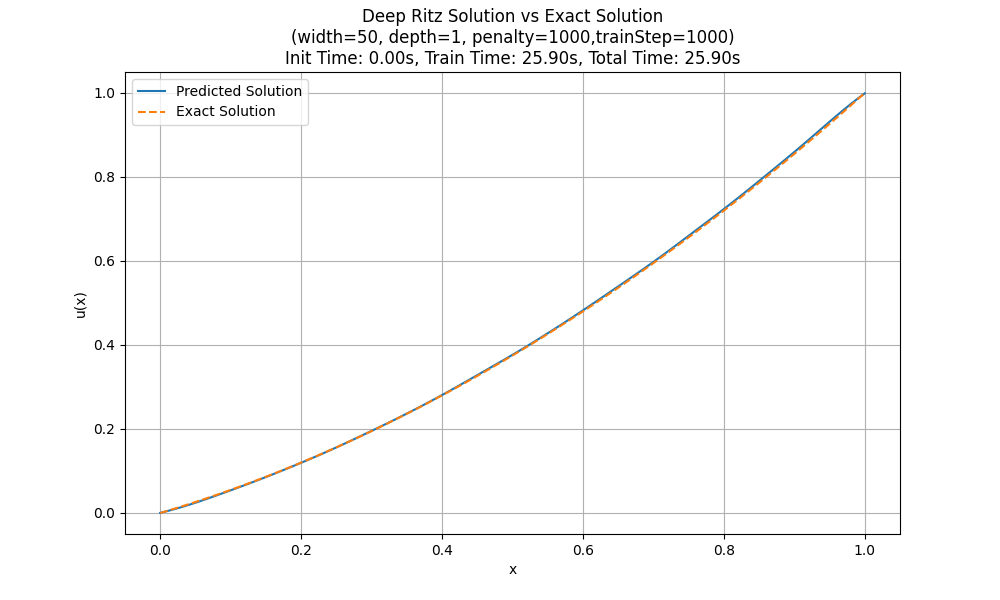
\includegraphics[width=\textwidth, height=6cm, keepaspectratio]{figures/5-1-1.png}
        \caption{RKPM方法L2误差}
        \label{fig:deepritz_solutions}
    \end{subfigure}
    \hfill
    \begin{subfigure}[b]{0.45\textwidth}
        \centering
        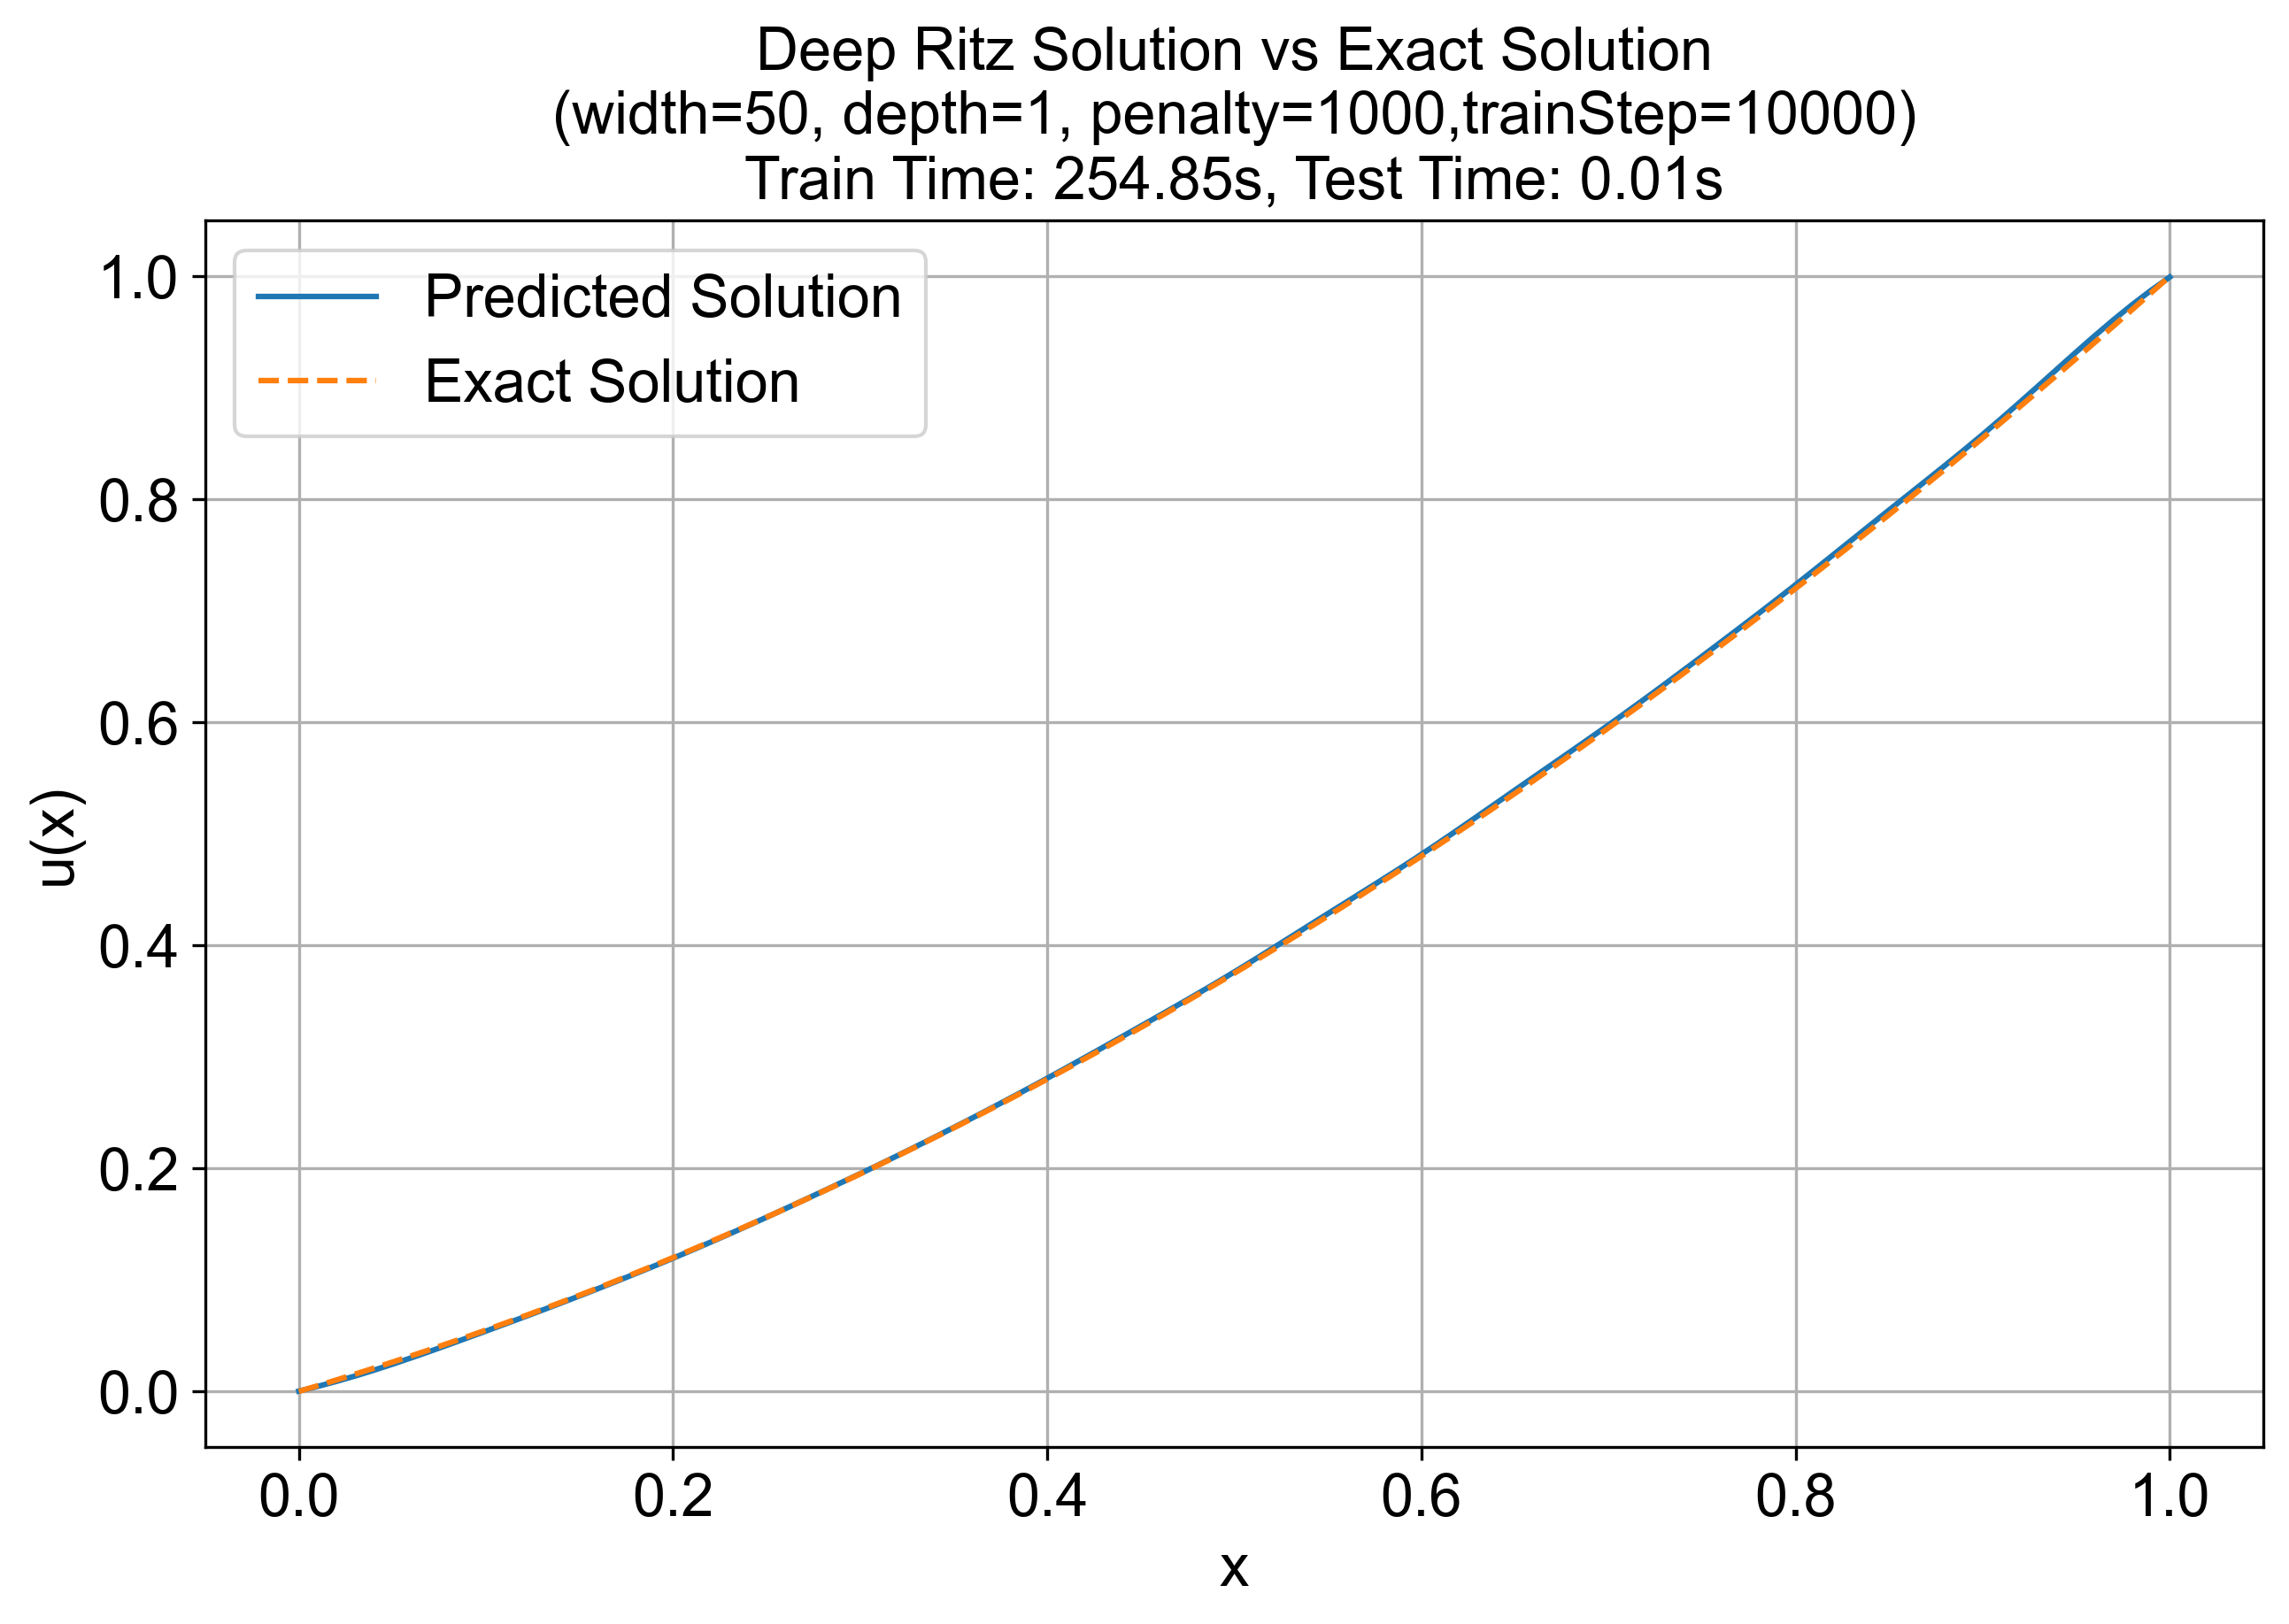
\includegraphics[width=\textwidth, height=6cm, keepaspectratio]{figures/5-2-1.png}
        \caption{再生核增强10000步L2误差}
        \label{fig:absolute_error}
    \end{subfigure}

    \centering
    \caption{L2误差对比}
    \label{fig:combined}
\end{figure}
\end{comment}

\chapter{算例分析}
在深度 里兹 方法的训练过程中，为了避免过拟合或不必要的计算，我们设计了一个基于损失函数收敛性的停止机制。该机制通过监控最近若干步的损失值变化来判断模型是否已达到稳定状态，并在满足条件时提前终止训练。

设训练过程中的损失函数为 \( L(\theta) \)，其中 \( \theta \) 表示模型参数。停止机制的核心思想是：在连续的 \( w \) 步（称为窗口大小）内，如果损失值的最大变化小于预设阈值 \( \tau \)，则认为模型已收敛，训练应停止。

在实现中，我们设置：窗口大小 \( w = 100 \)，收敛阈值 \( \tau = 10^{-5} \)。

考虑\eqref{eq:poisson_strong}两端固定的一维弹性杆问题，即
\[
    \left\{
    \begin{array}{ll}
        \nabla^2 u - q = 0 & \mathrm{in~} (0, l) \\
        u(0) =u(1)= 0 
    \end{array}
    \right.
    \label{eq:strong_form1}
\]

该问题的解析解为：
\begin{equation}
u(x) = \frac{x^2}{2} + \frac{x}{2}
\label{eq:analytical_solution}
\end{equation}

基于该一维问题构建一个深度神经网络，其中输入和输出维度分别为 1，网络包含宽度为 50 且深度为 1（总层数为 3）的全连接层，采用 $\tanh$ 激活函数；其次，利用 100 个内部采样点和 2 个边界点构造损失函数，其中体积分损失基于拉普拉斯方程的变分形式 $\int_0^1 \left( \frac{1}{2} |\frac{\partial u}{\partial x}|^2 - f u \right) dx$ 近似计算，边界损失通过惩罚系数 1000 强制满足 Dirichlet 边界条件 $u(0)=0$ 和 $u(1)=1$；




再生核增强里兹方法采用增强模块，通过 11 个均匀分布的节点（间距 0.1）及支持域大小 0.2 的三次样条核函数，计算形状函数并将其与原始输入拼接，增强网络特征表达；

采用 Adam 优化器以初始学习率 0.001，讨论两方法在不同SteoLR调度测略下的收敛情况，如图\ref{fig:stepsize} 所示 DR方法取步长为5000，RKDR方法取步长为300，获得最快损失函数收敛速度。此外，DR 方法和RKDR方法损失函数最终稳定在 0.96 左右，DR损失下降过程较为平滑，在约 12000 步时收敛。RKDR 方法损失迅速下降，在600步左右收敛，且收敛后的损失值更低。



\begin{figure}[htbp]
    \centering
    \begin{subfigure}[b]{0.48\textwidth}
        \centering
        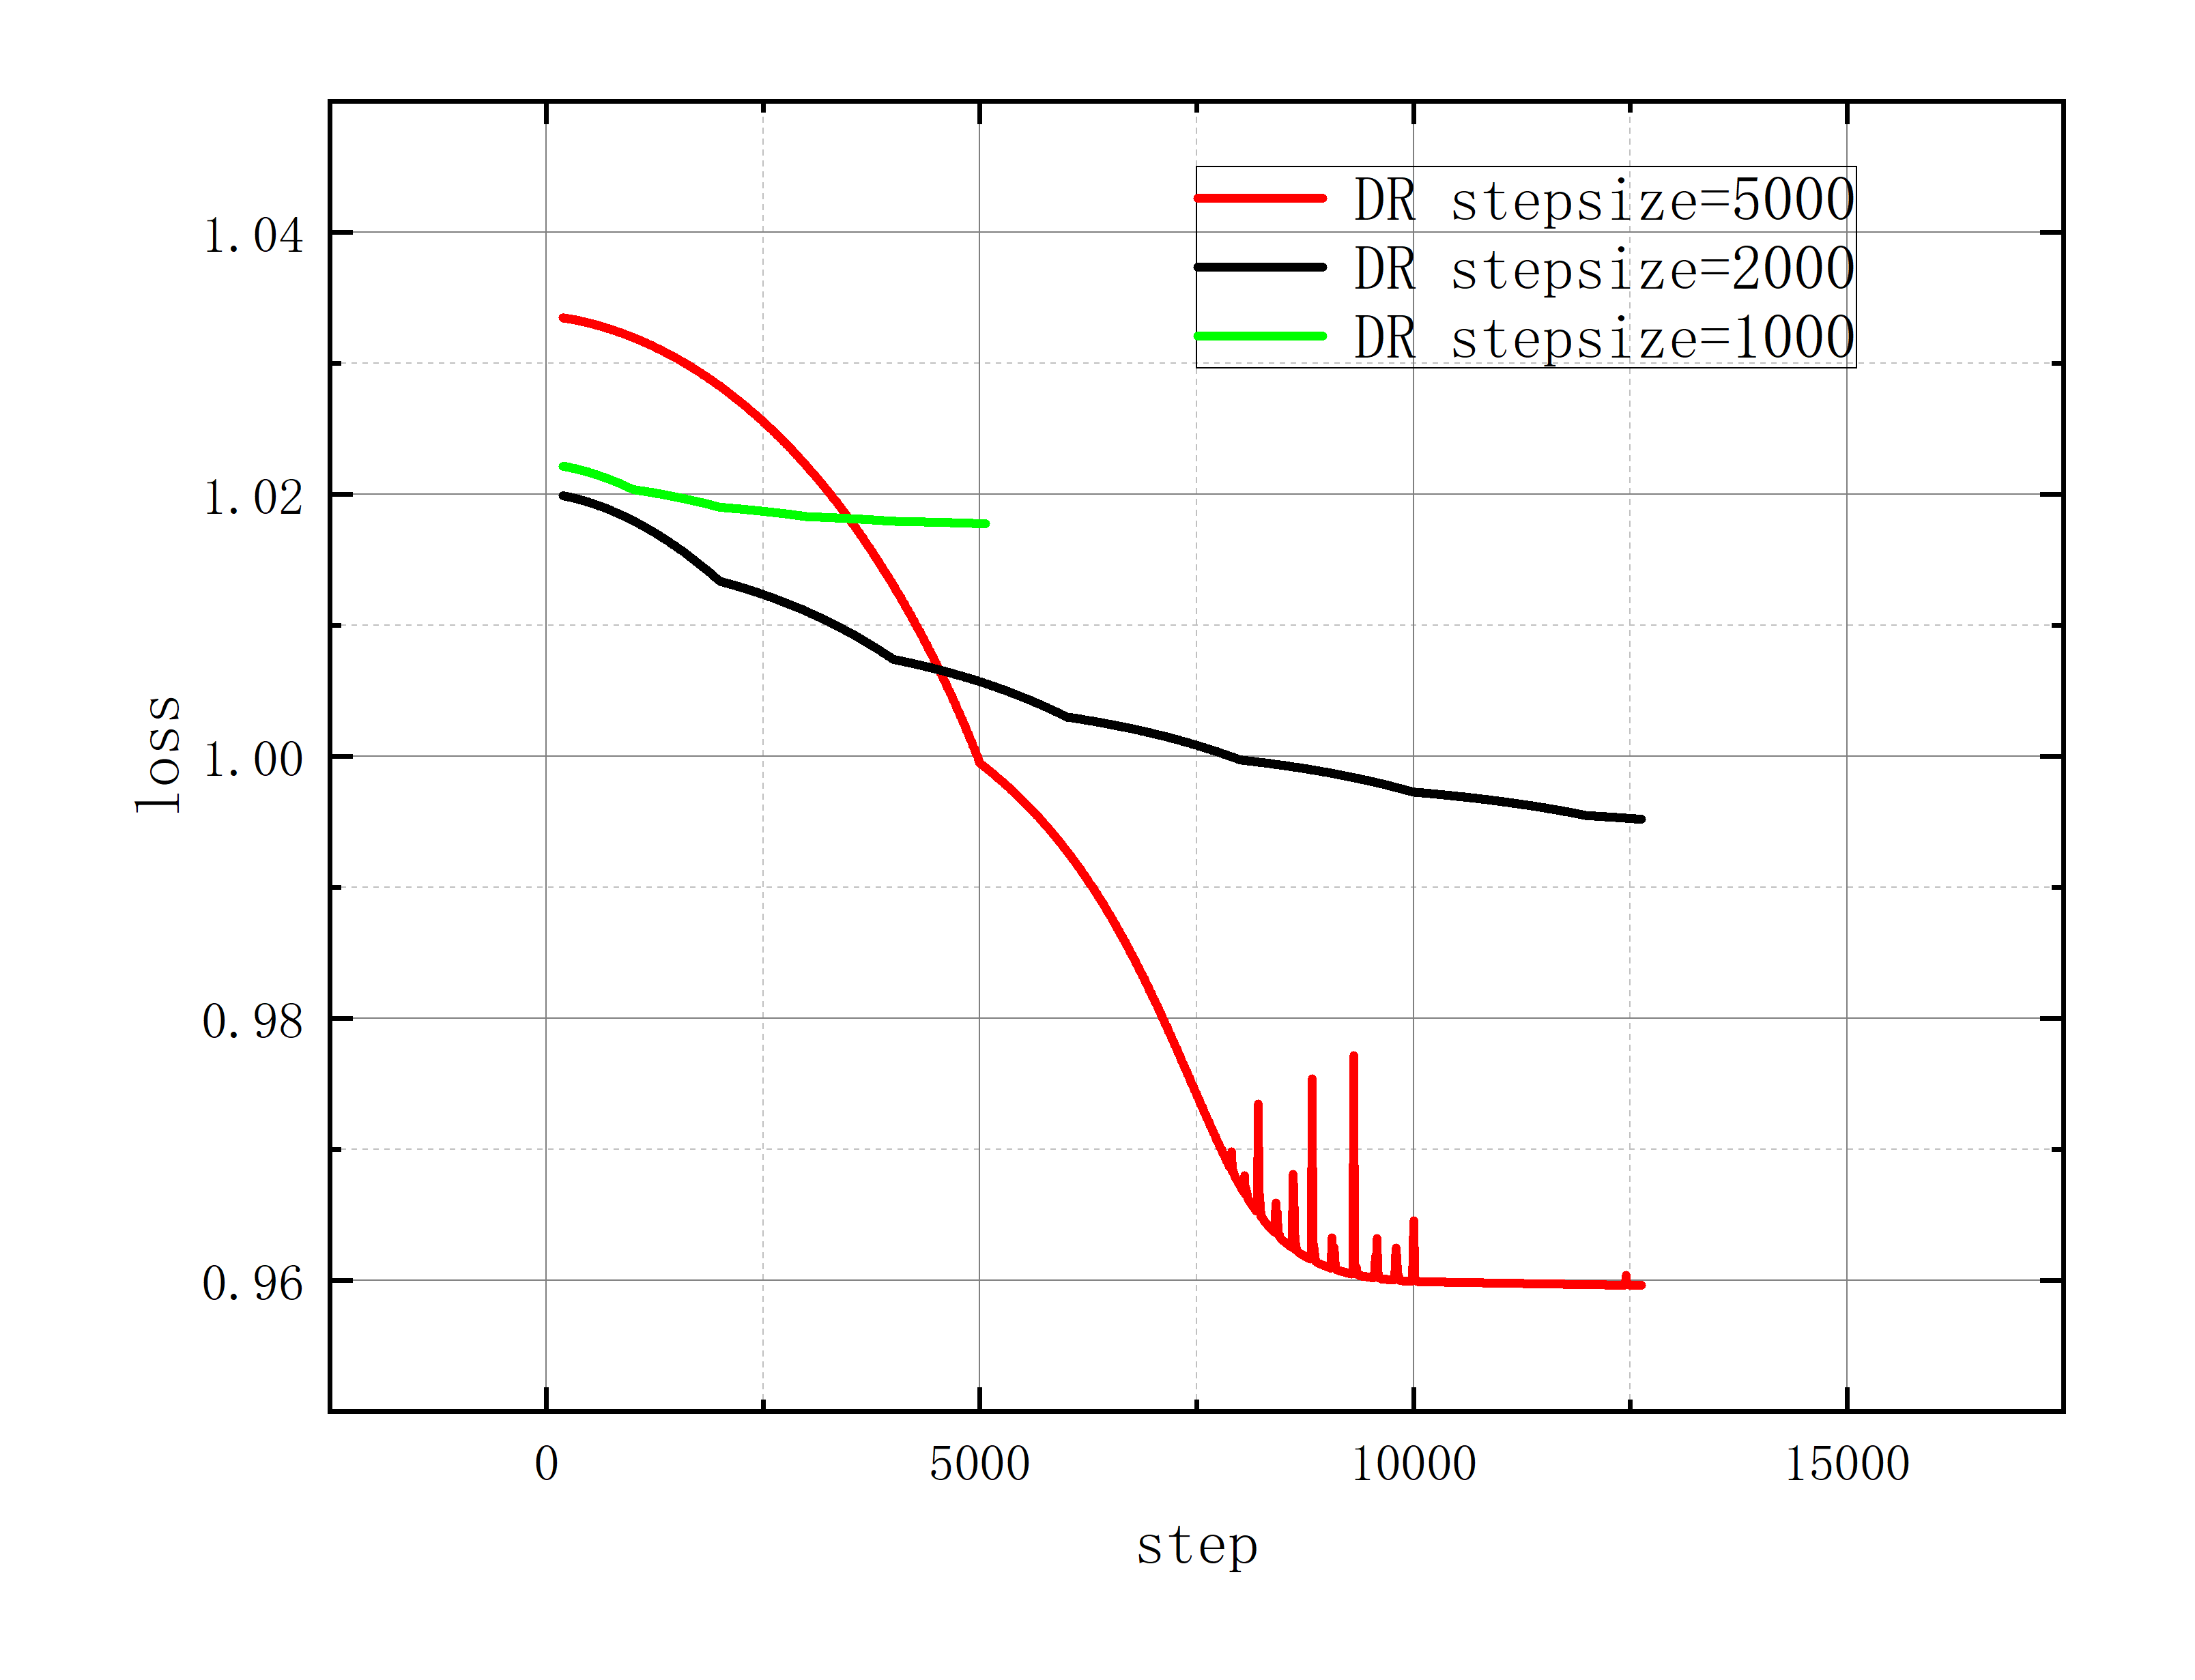
\includegraphics[width=\textwidth, height=6.5cm, keepaspectratio]{figures2/DRstepsize.png}
        \caption{DR方法收敛步数}
        \label{fig:3-4-3}
    \end{subfigure}
    \hspace{0.5em} % 减小水平间距
    \begin{subfigure}[b]{0.48\textwidth}
        \centering
        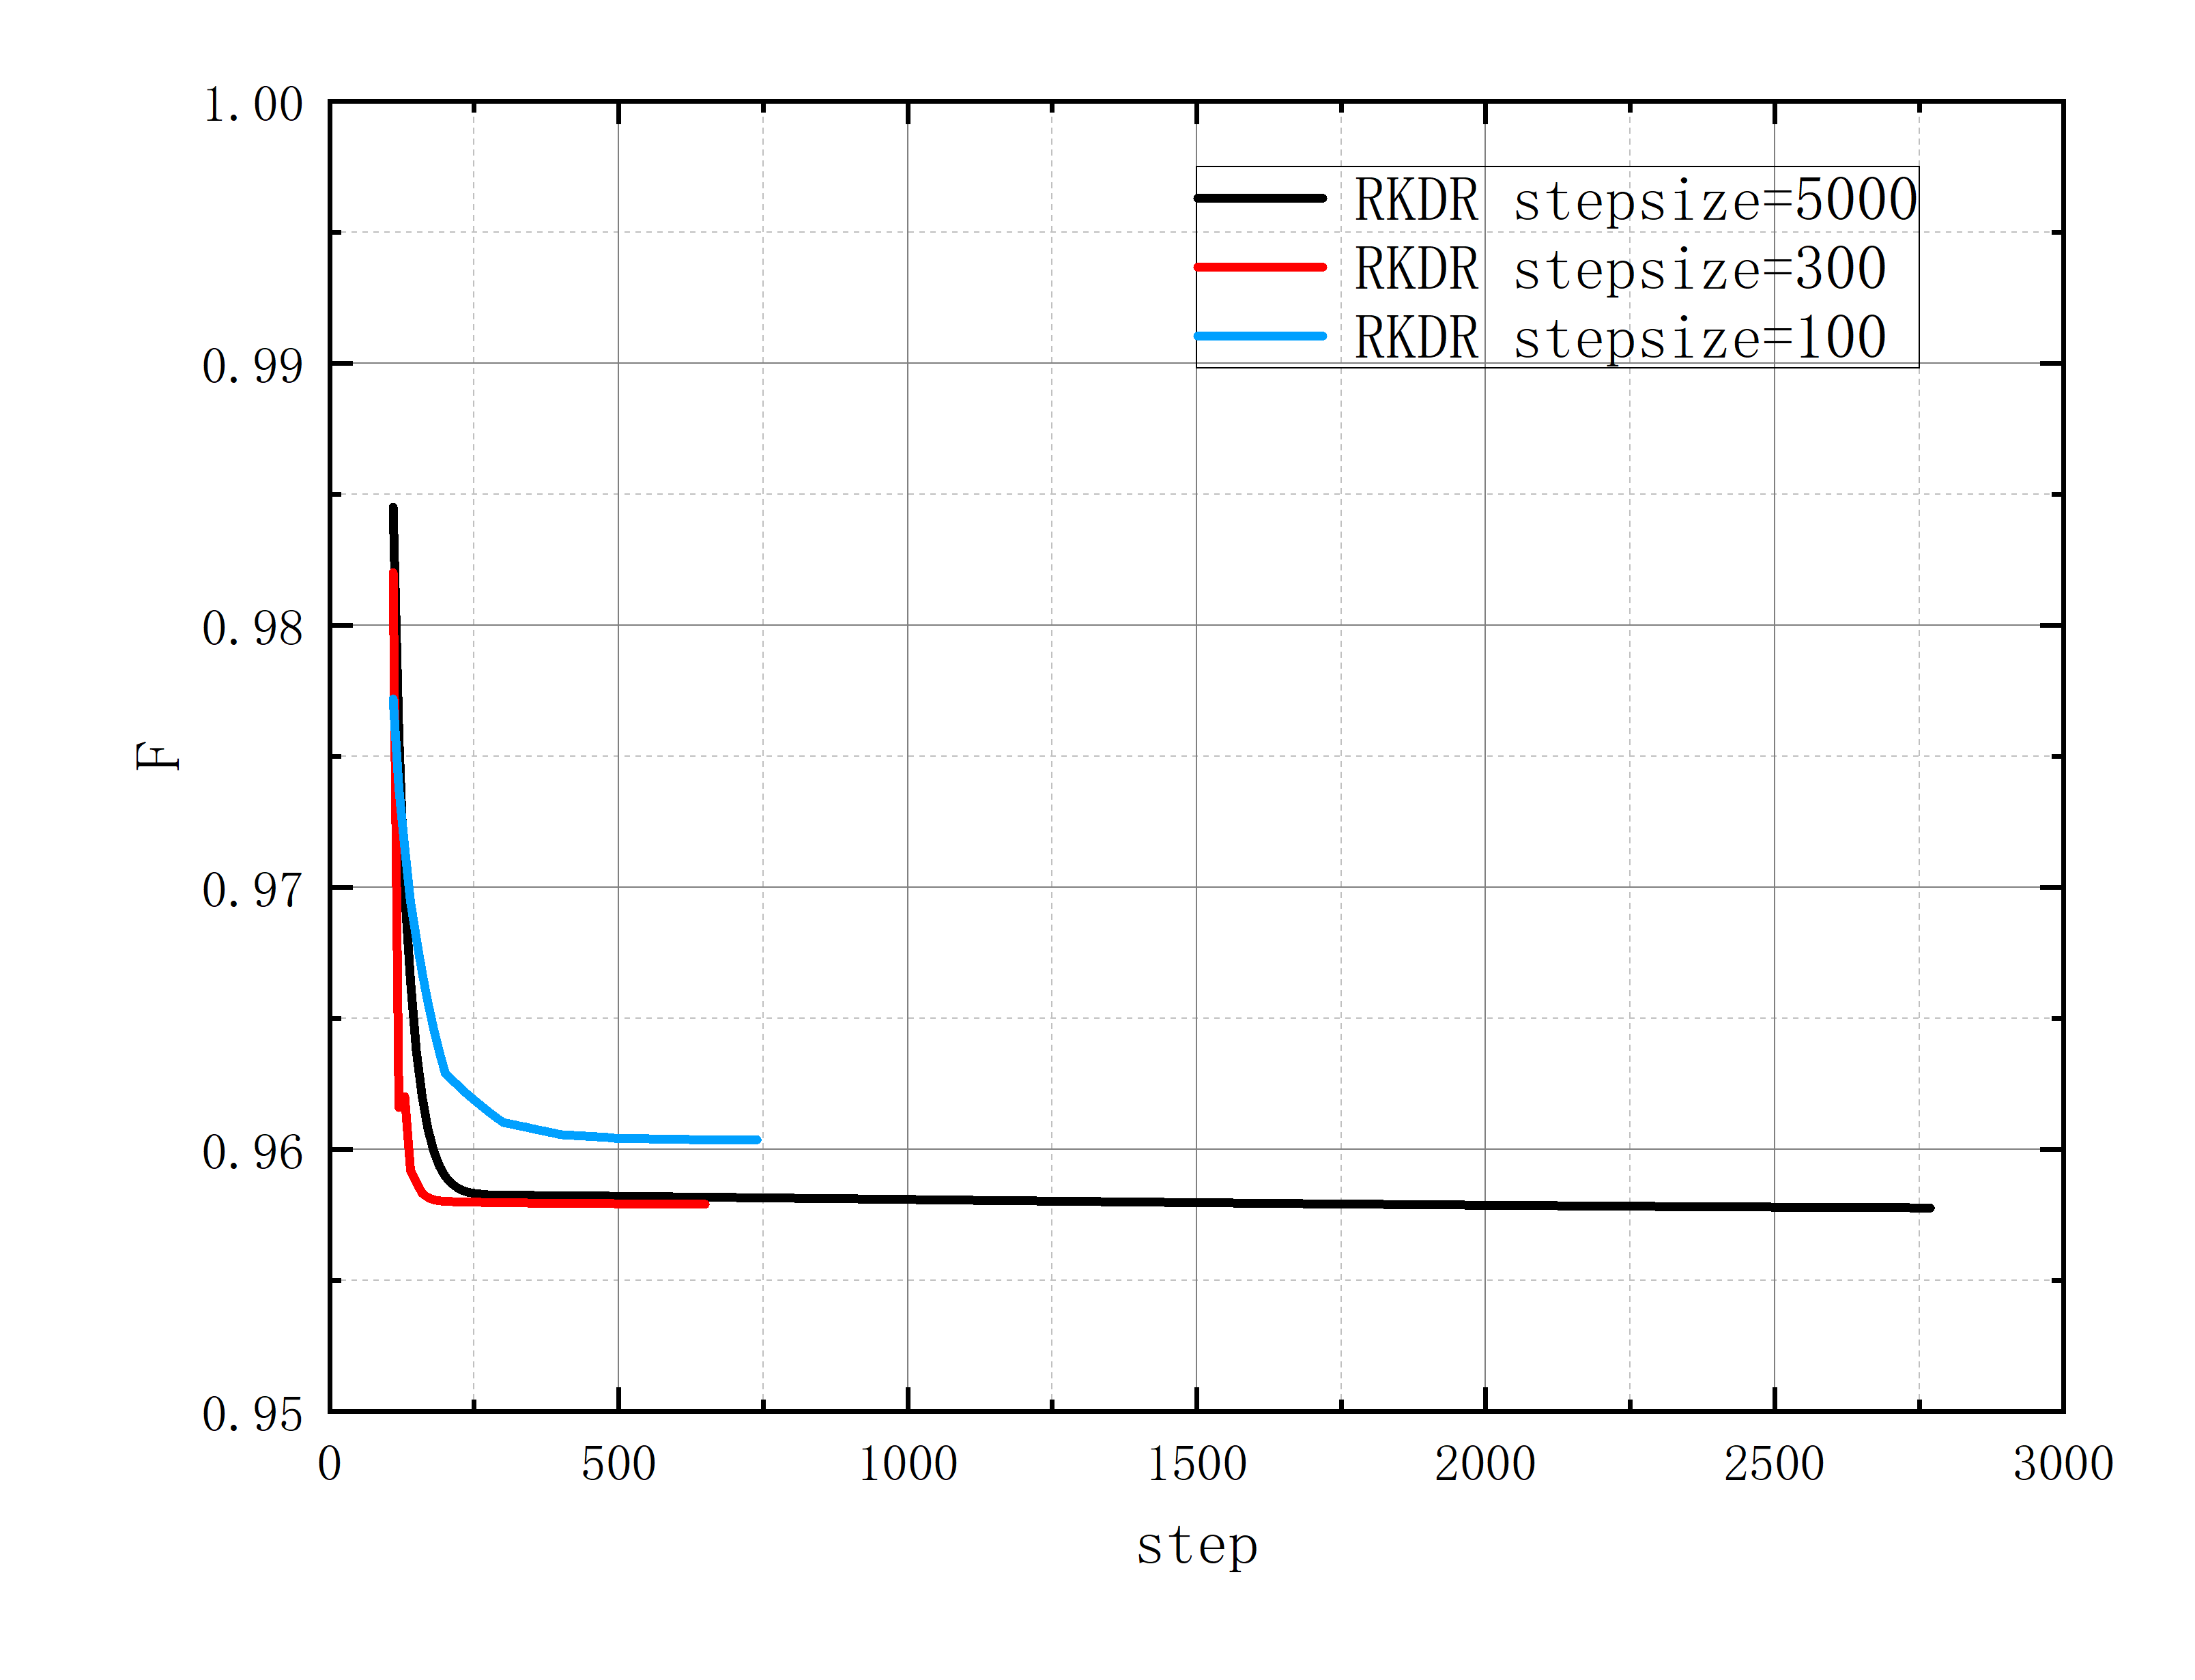
\includegraphics[width=\textwidth, height=6.5cm, keepaspectratio]{figures2/RKDRstepsize.png}
        \caption{RKDR方法收敛步数}
        \label{fig:5-3-4}
    \end{subfigure}

    \caption{两方法收敛损失函数图像}
    \label{fig:stepsize}
\end{figure}


为了对比深度 里兹 方法（DR）和增强深度 里兹 方法（RKDR）在相同训练步数下的收敛性能，我们将两种方法的训练步数统一设置为 15000 步，并绘制损失随训练步数的变化曲线。
\begin{figure}[htbp]
    \centering
    \begin{subfigure}[b]{0.48\textwidth}
        \centering
        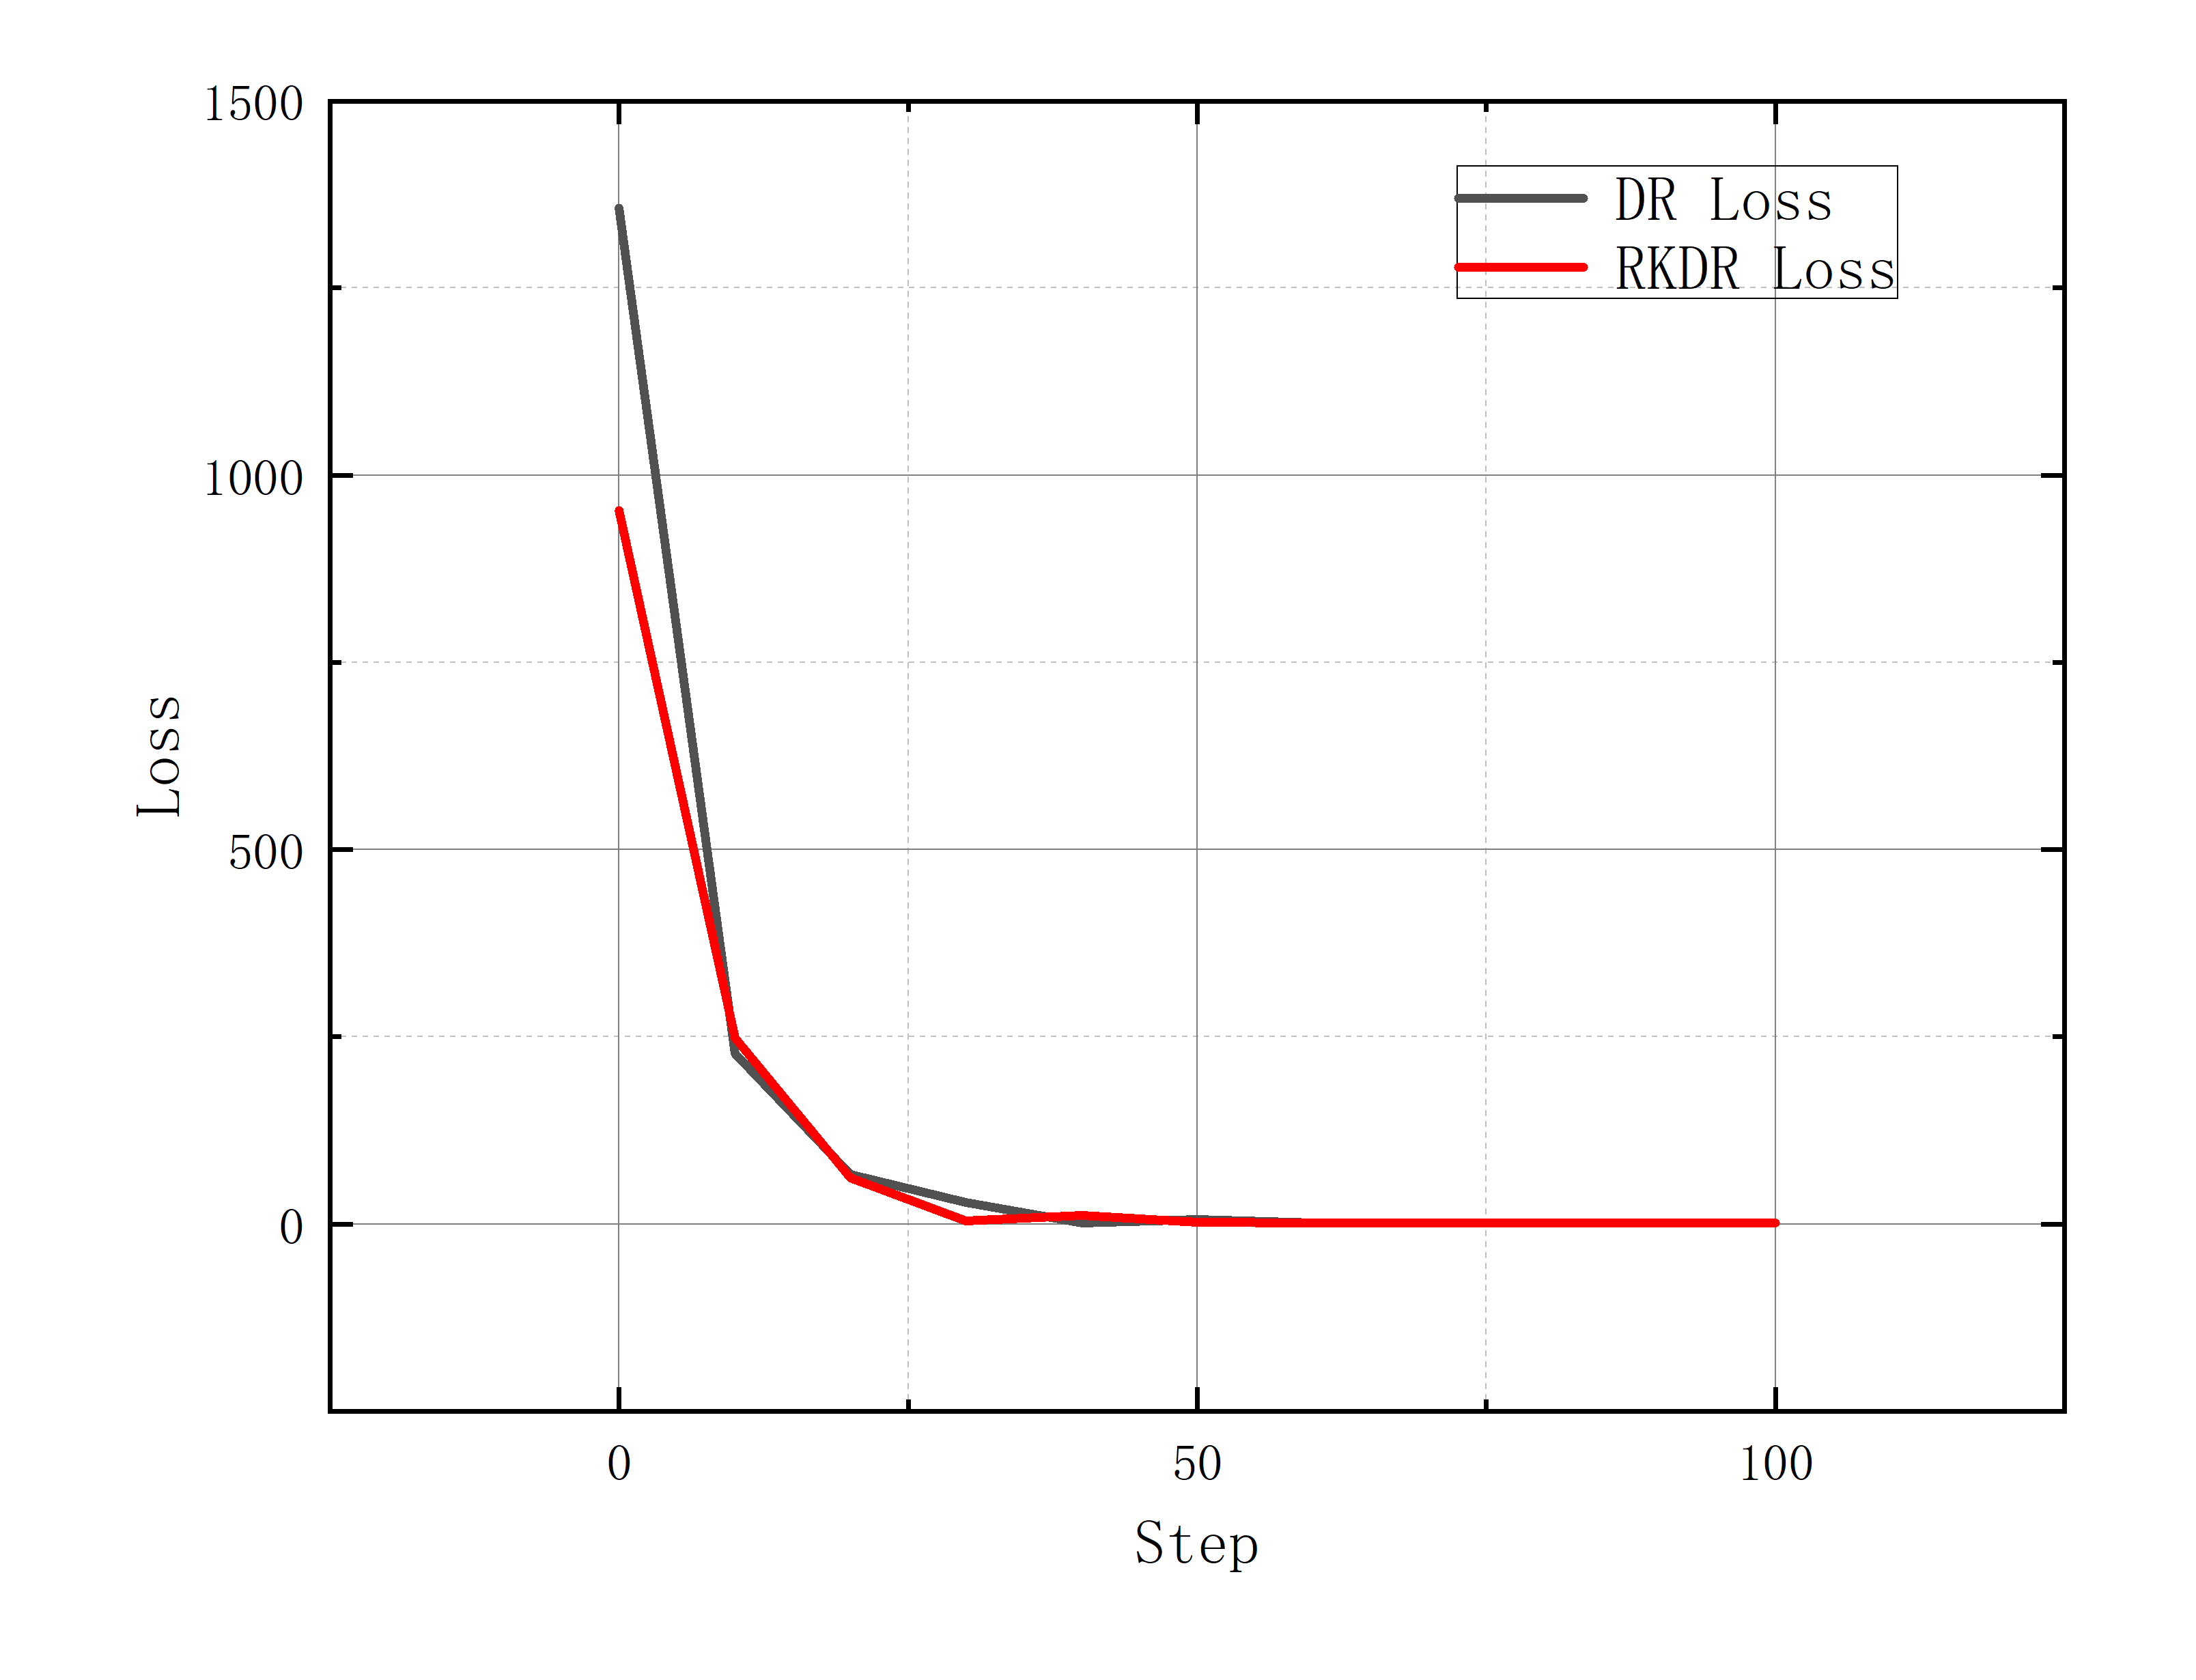
\includegraphics[width=\textwidth, height=6.5cm, keepaspectratio]{figures2/100stepsloss.png}
        \caption{0-100步损失函数对比}
        \label{fig:100stepsloss}
    \end{subfigure}
    \hspace{0.5em} % 减小水平间距
    \begin{subfigure}[b]{0.48\textwidth}
        \centering
        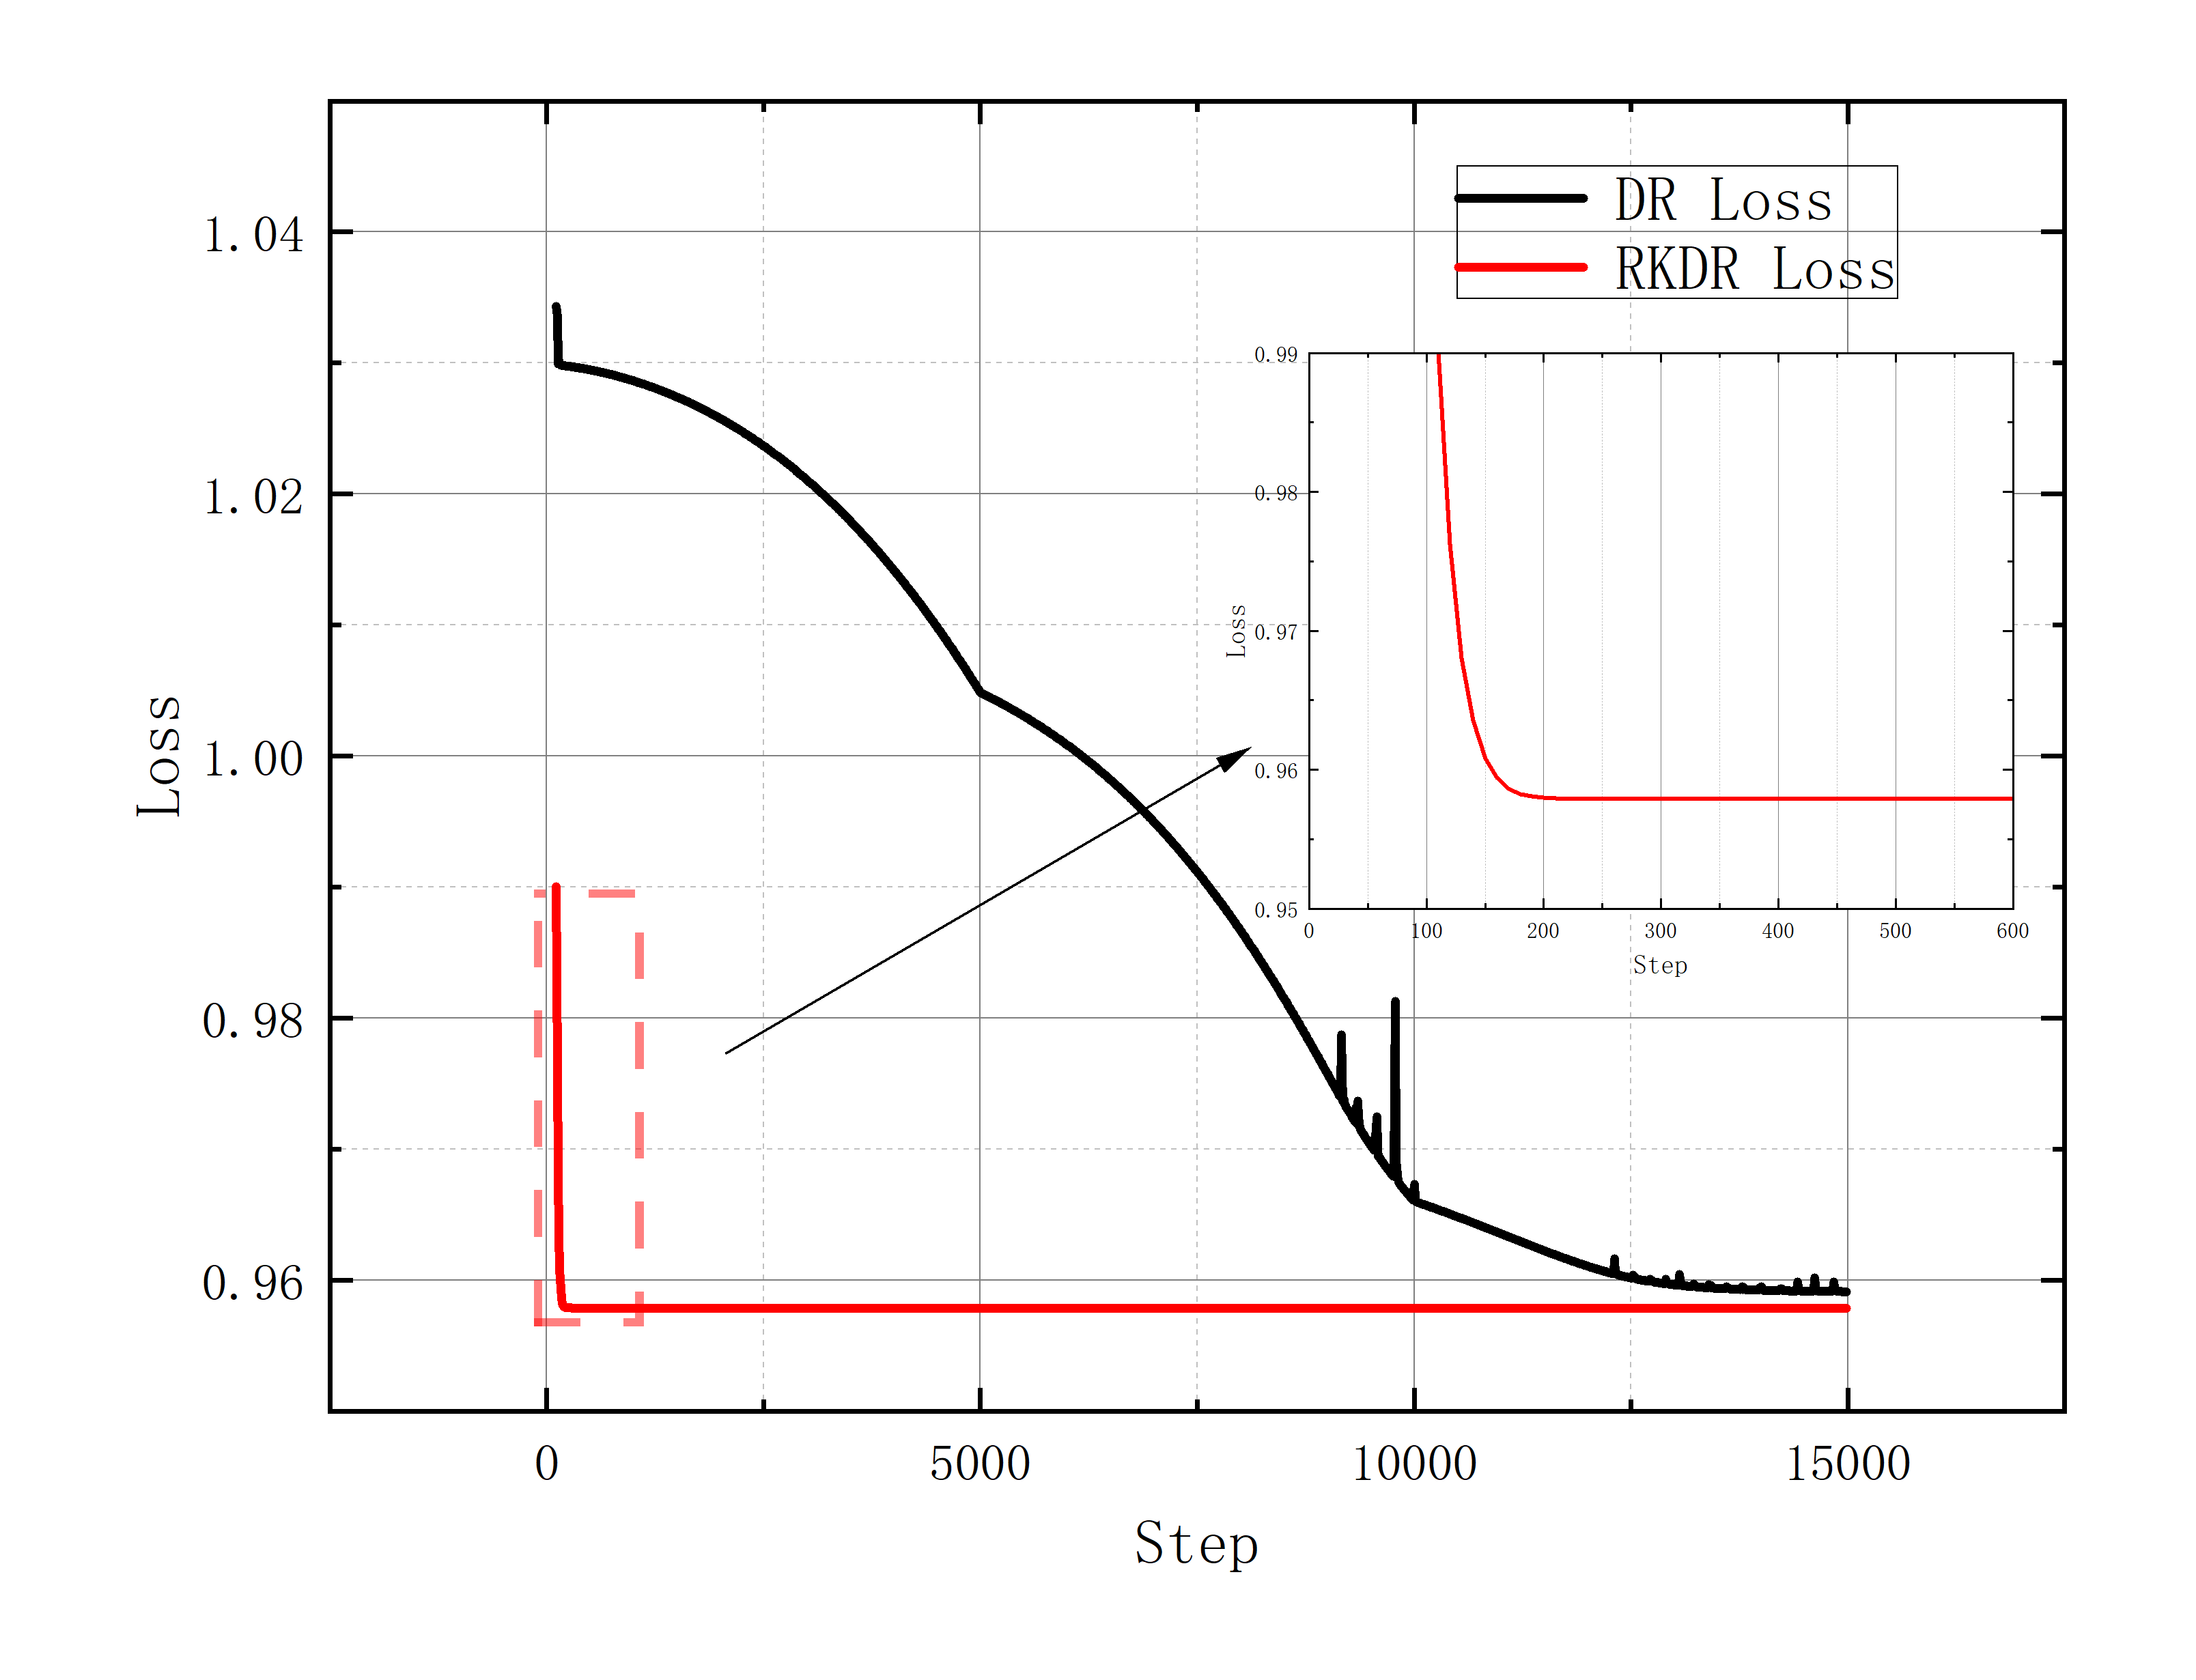
\includegraphics[width=\textwidth, height=6.5cm, keepaspectratio]{figures2/allstepsloss.png}
        \caption{100-15000步损失函数对比}
        \label{fig:allstepsloss}
    \end{subfigure}

    \caption{15000步损失函数图像}
    \label{fig:combined_loss}
\end{figure}


图 \ref{fig:combined_loss} a显示，在前 100 步内，RKDR 方法的初始损失较低，但两者的下降速度相似，最终在 100 步左右都下降到 1，表明在训练初期两者的优化效率相当。

图 \ref{fig:combined_loss} b显示，RKDR 方法从第 100 步到第 200 步，损失快速下降至0.96，几乎没有波动，表明 RKDR 方法在 200 步后已完全收敛，表现出极高的稳定性。
而DR方法在 100 步到 15000 步之间，损失继续缓慢下降，最终在 15000 步左右稳定在 0.96 左右，但存在微小波动，尤其在 5000 步到 10000 步之间有轻微起伏。

在图 \ref{fig:abs_error} 中，我们对比了 DR 和 RKDR 方法的绝对误差分布。对于 DR 方法，其绝对误差在 \( x \in [0, 0.2] \) 和 \( x \in [0.8, 1.0] \) 区域内较小，但在 \( x \in [0.2, 0.8] \) 区域内波动较大，最大误差接近 0.14，特别是在 \( x \approx 0.5 \) 附近达到峰值。这表明 DR 方法对解的全局拟合不足。相比之下，RKDR 方法的绝对误差整体波动较小，最大误差仅约为 0.06，远低于 DR 方法。RKDR 的误差分布较为均匀，没有明显的峰值，表明其在整个定义域内对解的逼近更加一致和精确。说明RKDR 方法通过引入再生核增强，改善了神经网络的逼近能力，特别是在解的局部变化较大的区域（如 \( x \approx 0.5 \)），能够更好地捕捉解的细节，从而显著减小绝对误差。

图 \ref{fig:gradient_error} 展示了梯度误差的对比结果。梯度误差反映了解的导数逼近精度，RKDR 方法通过再生核的数学完备性，增强了神经网络对导数的拟合能力，特别是在边界附近和解变化剧烈的区域，表现出更高的精度和稳定性。

\begin{comment}


\begin{figure}[htbp]
    \centering
    \begin{subfigure}[b]{0.48\textwidth}
        \centering
        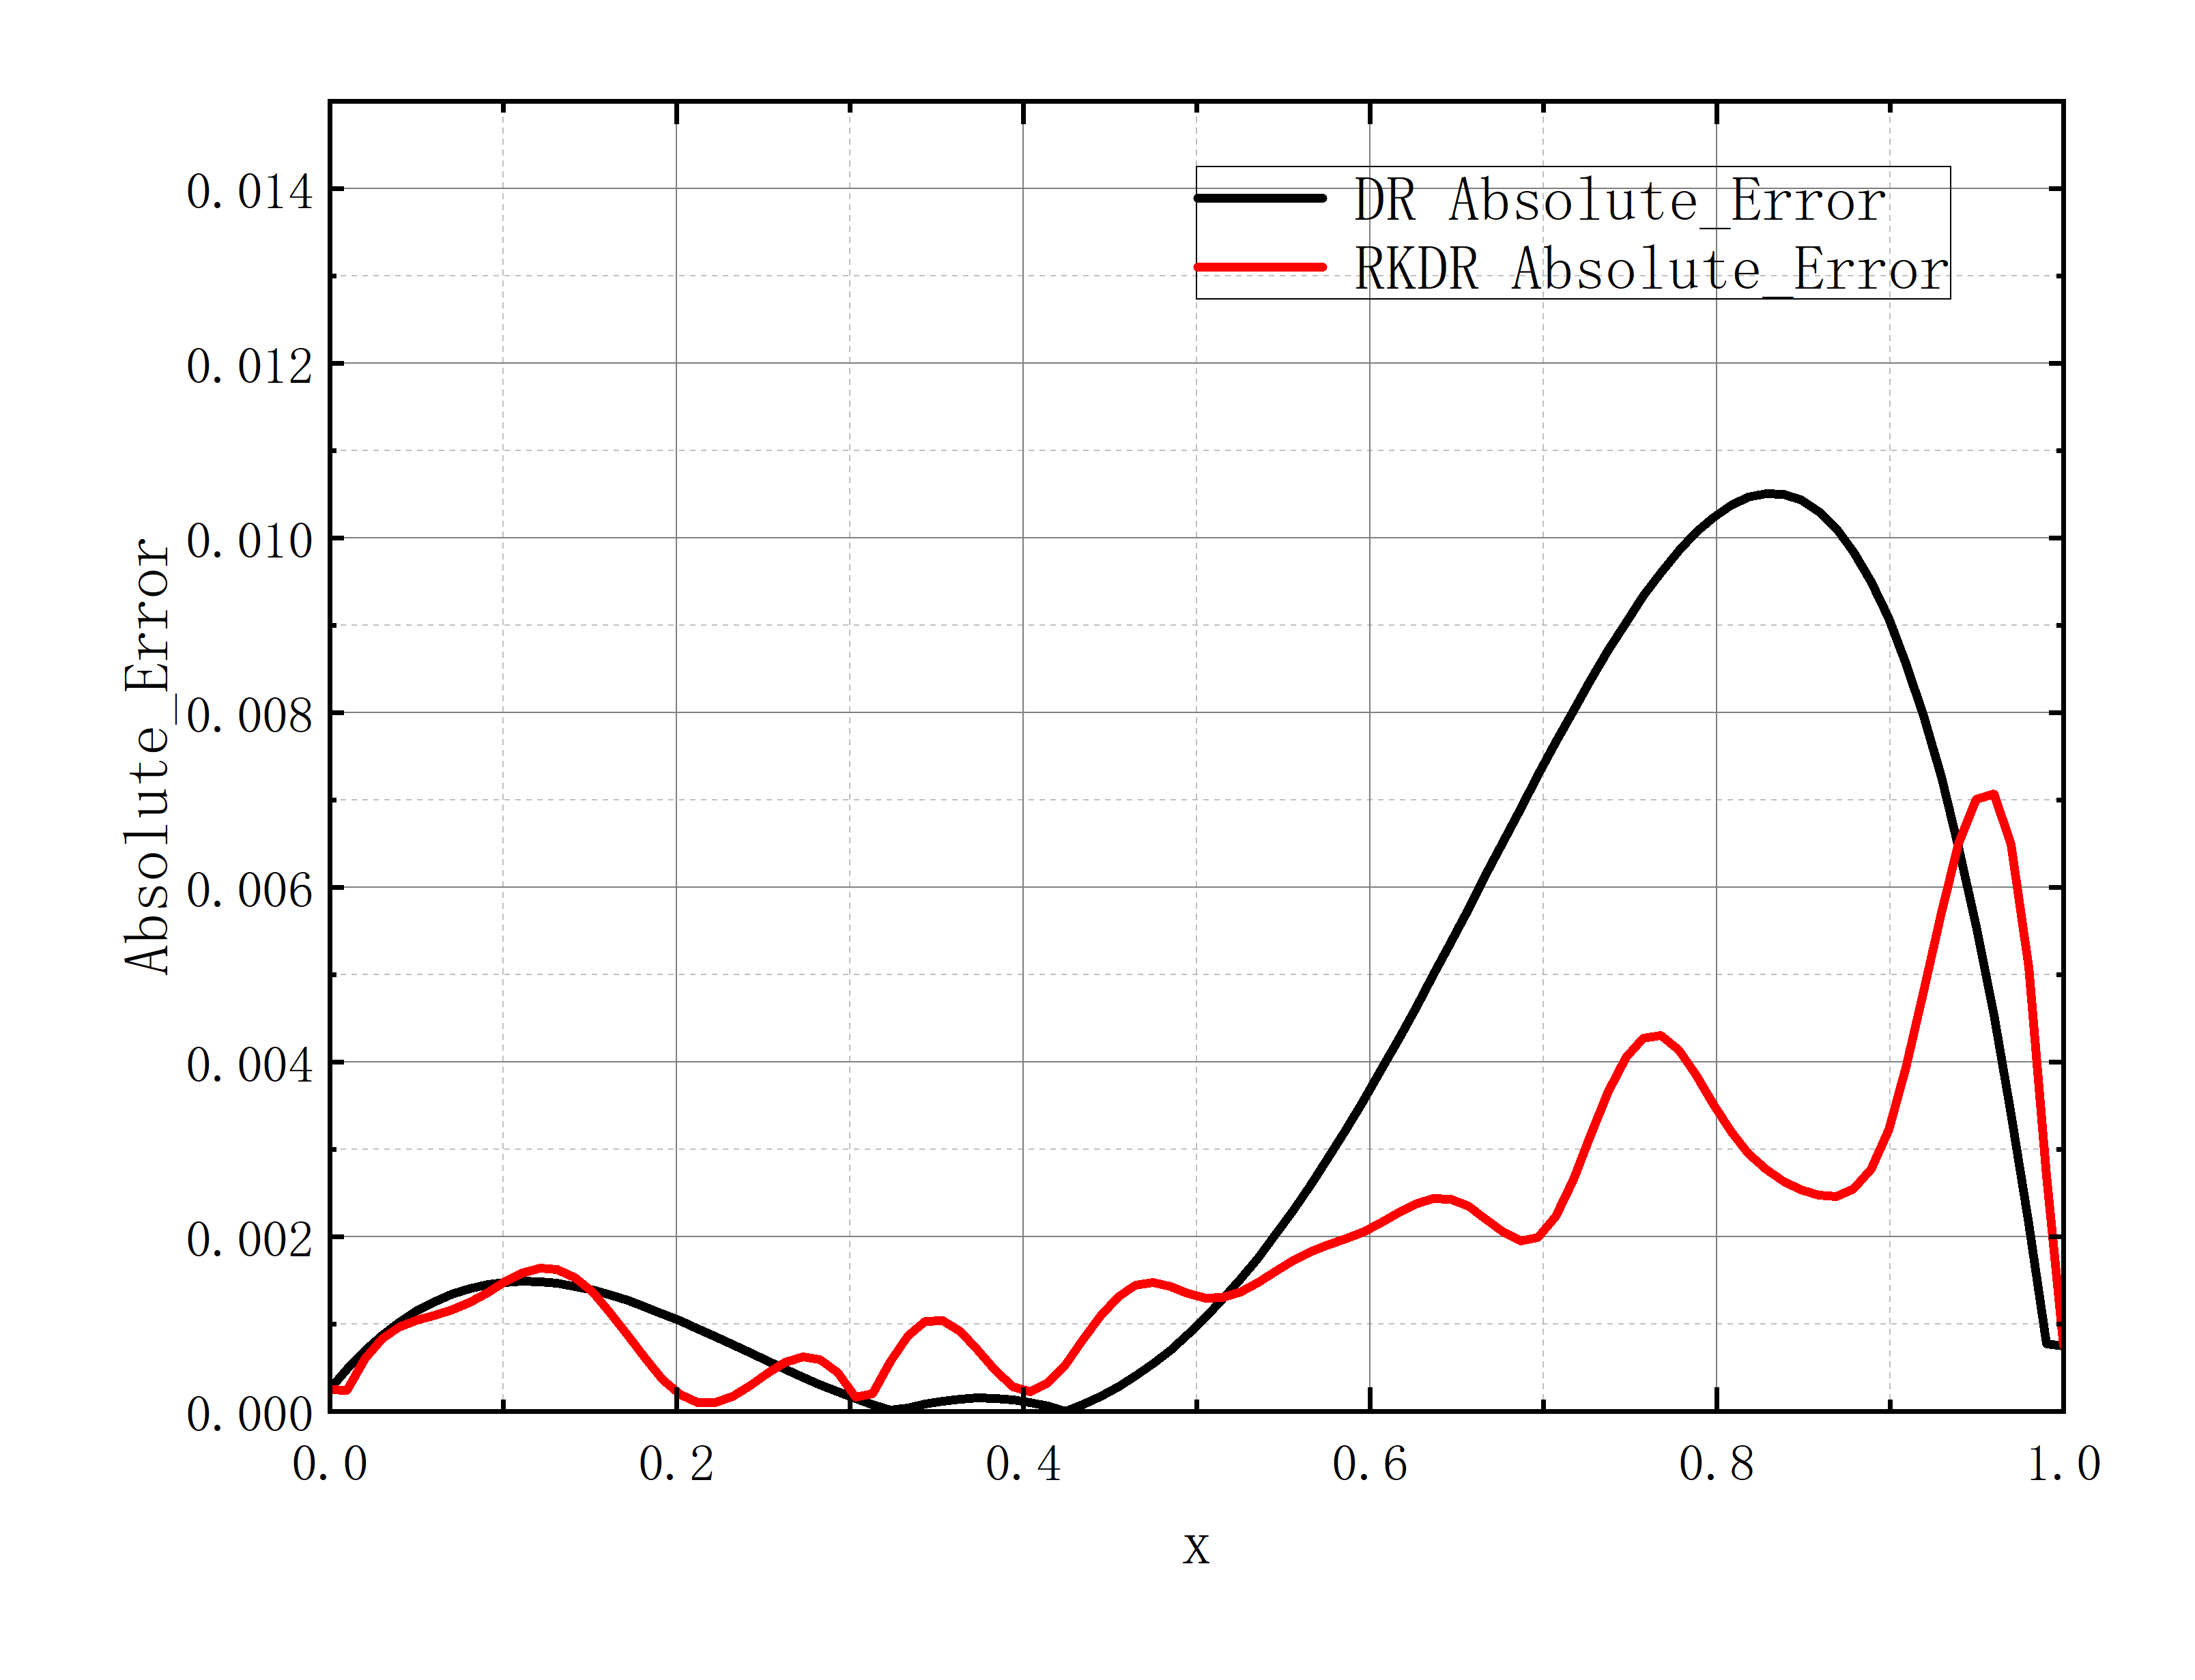
\includegraphics[width=\textwidth, height=6.5cm, keepaspectratio]{figures2/Abserror.png}
        \caption{绝对误差对比}
        \label{fig:abs_error}
    \end{subfigure}
    \hspace{0.5em} % 减小水平间距
    \begin{subfigure}[b]{0.48\textwidth}
        \centering
        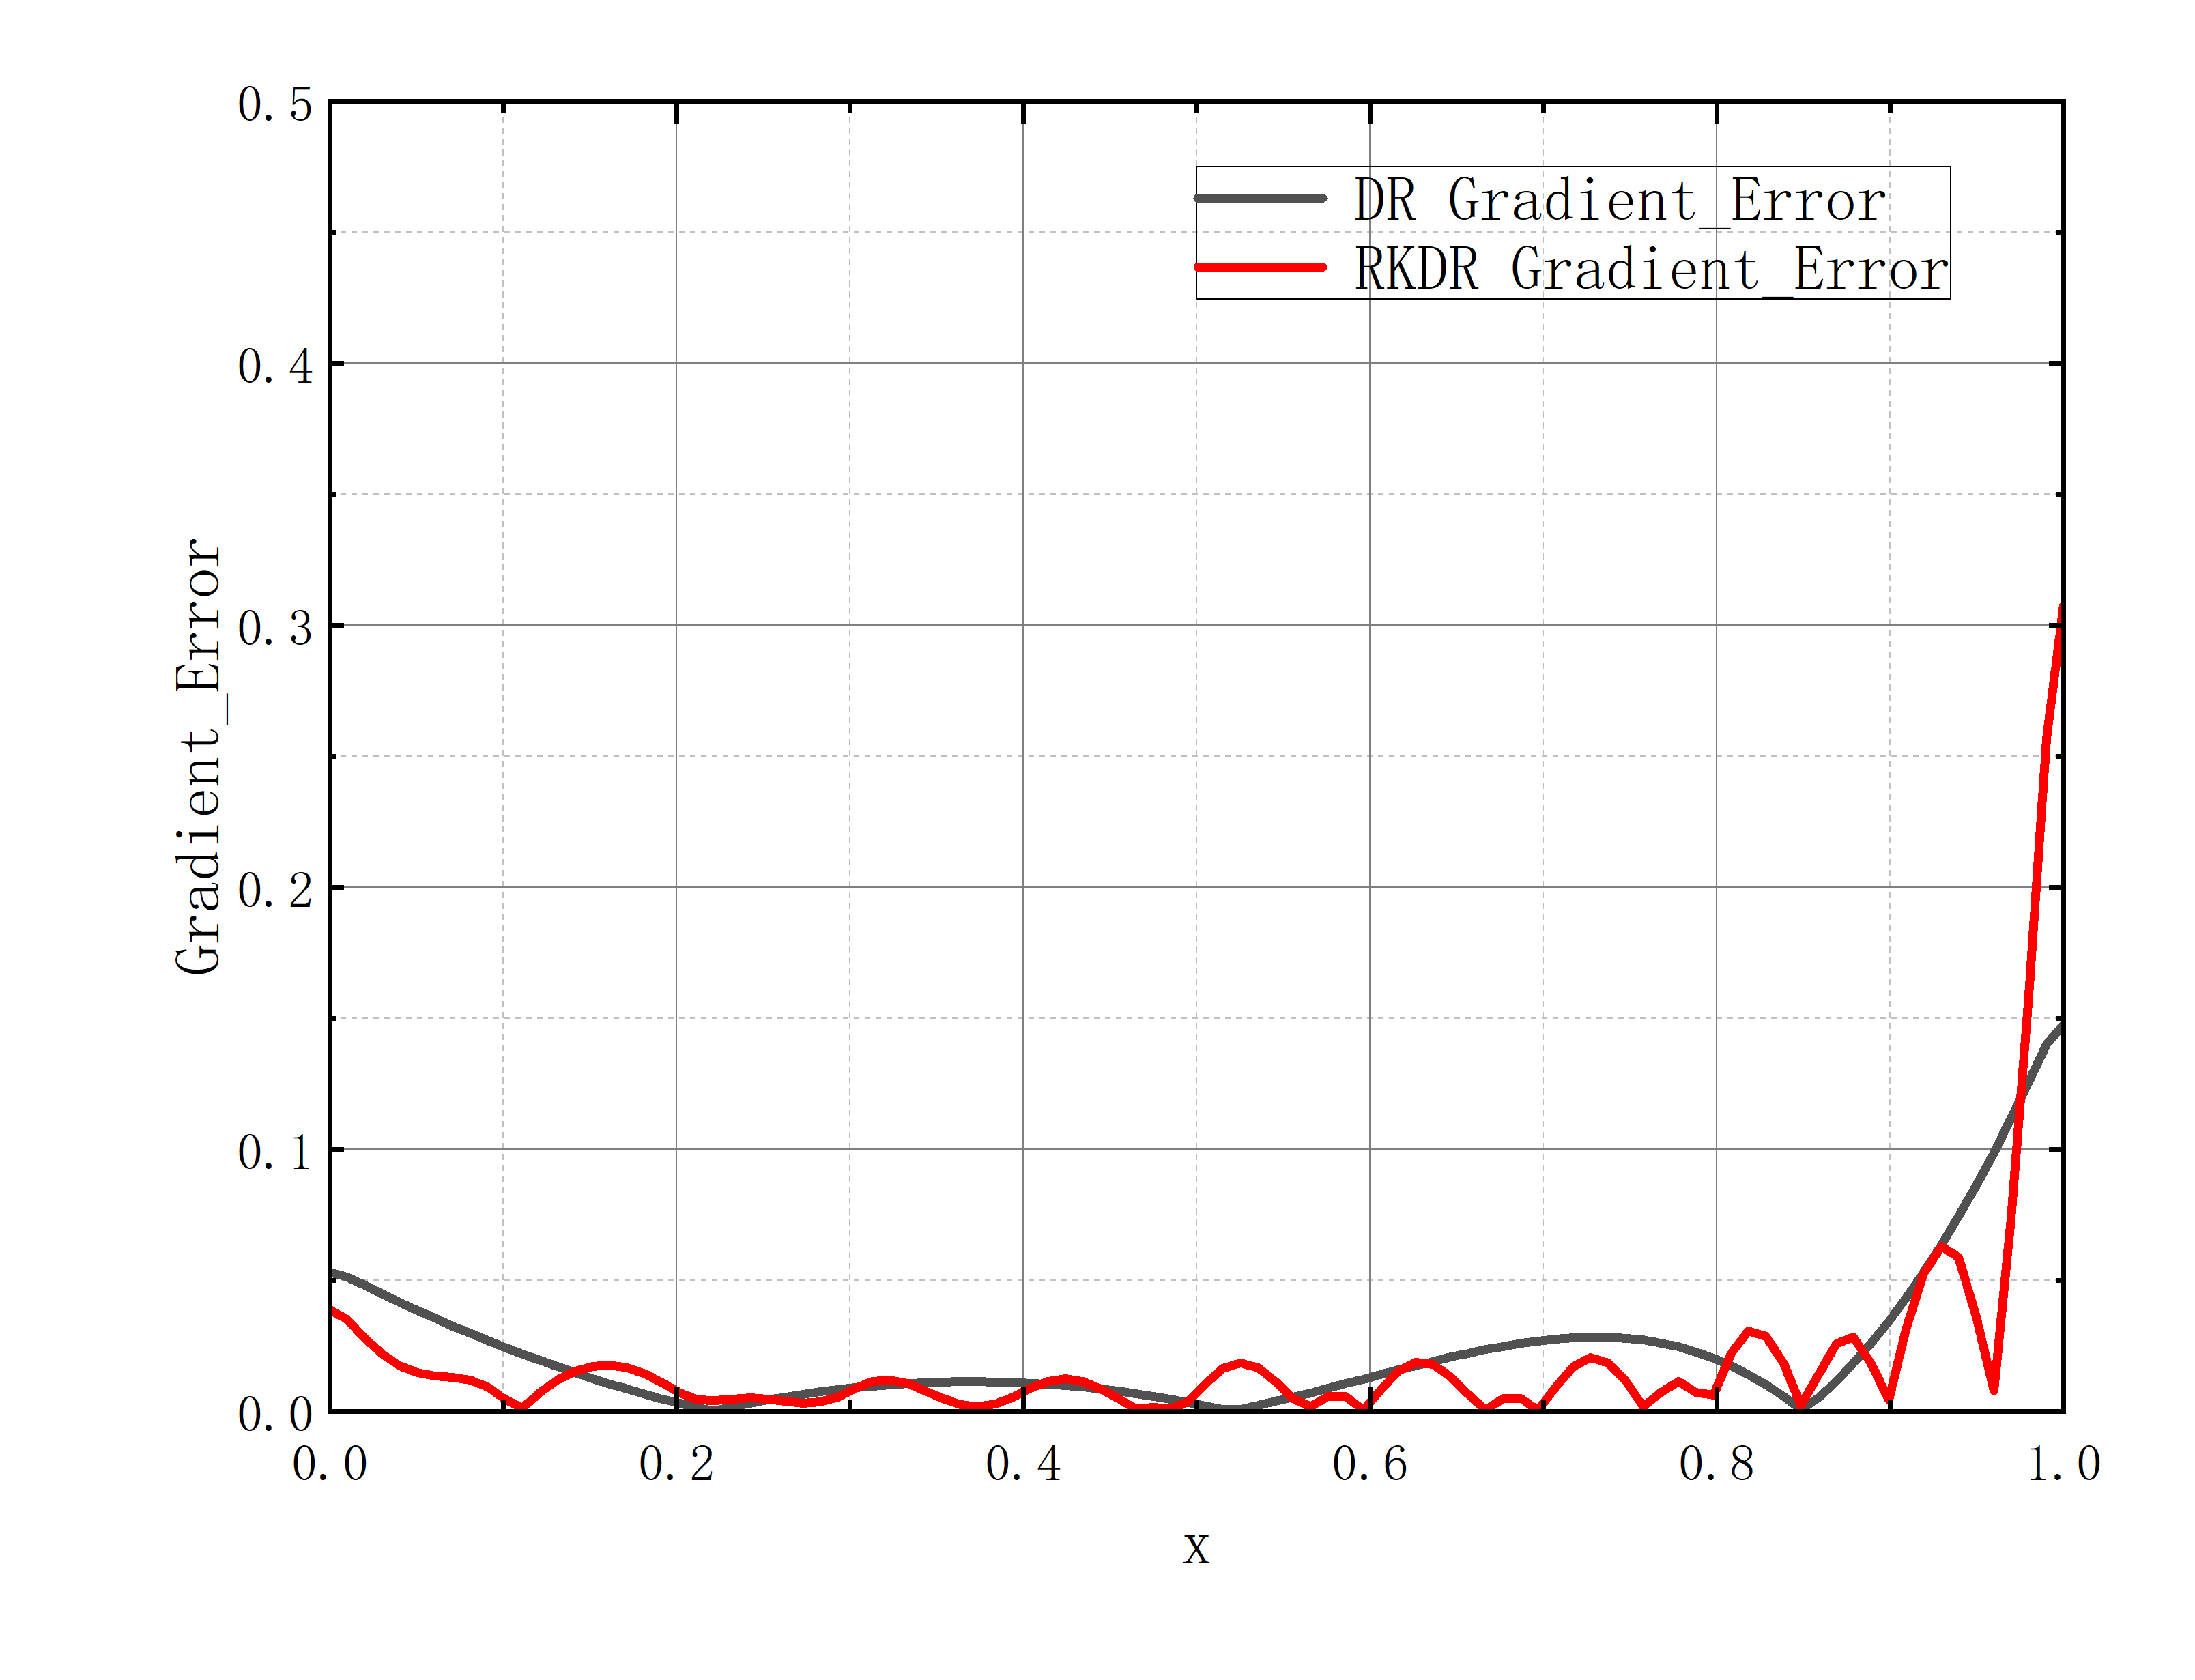
\includegraphics[width=\textwidth, height=6.5cm, keepaspectratio]{figures2/gradienterror.png}
        \caption{梯度误差对比}
        \label{fig:gradient_error}
    \end{subfigure}

    \vspace{1em} % 控制两行子图之间的垂直间距
    \begin{subfigure}[b]{0.48\textwidth}
        \centering
        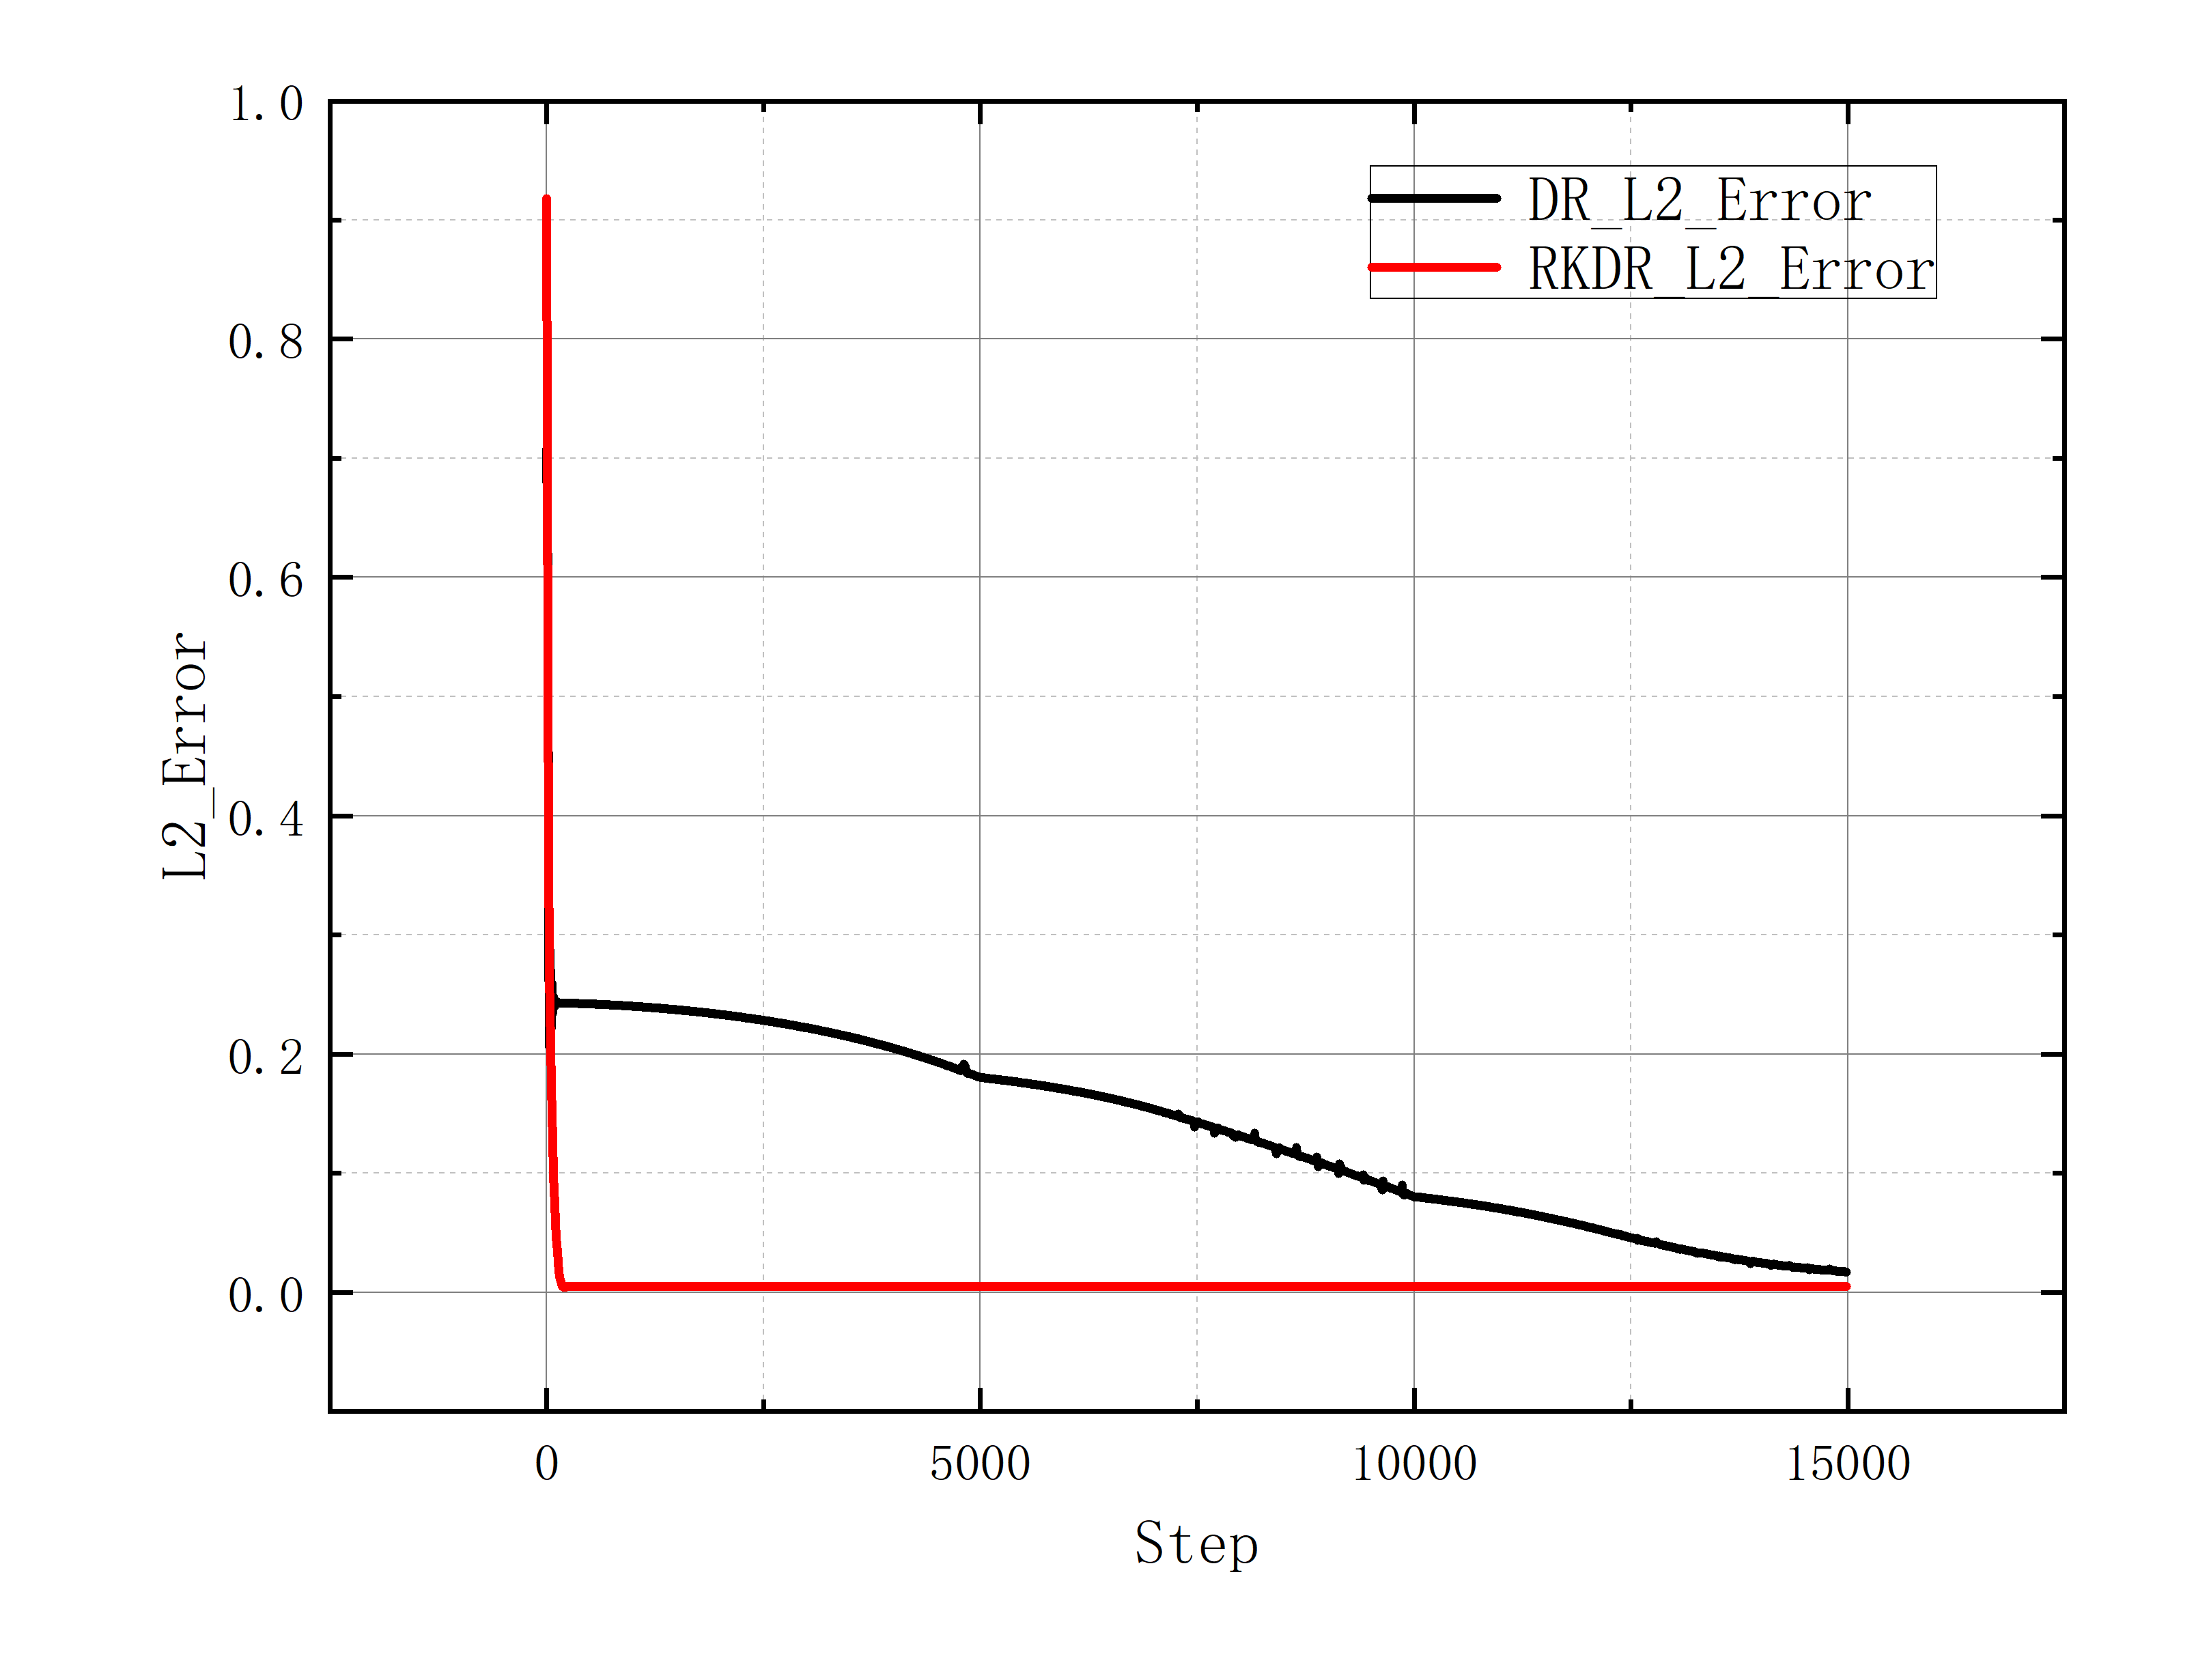
\includegraphics[width=\textwidth, height=6.5cm, keepaspectratio]{figures2/l2error.png}
        \caption{L2误差变化}
        \label{fig:l2_error}
    \end{subfigure}
    \hspace{0.5em} % 减小水平间距
    \begin{subfigure}[b]{0.48\textwidth}
        \centering
        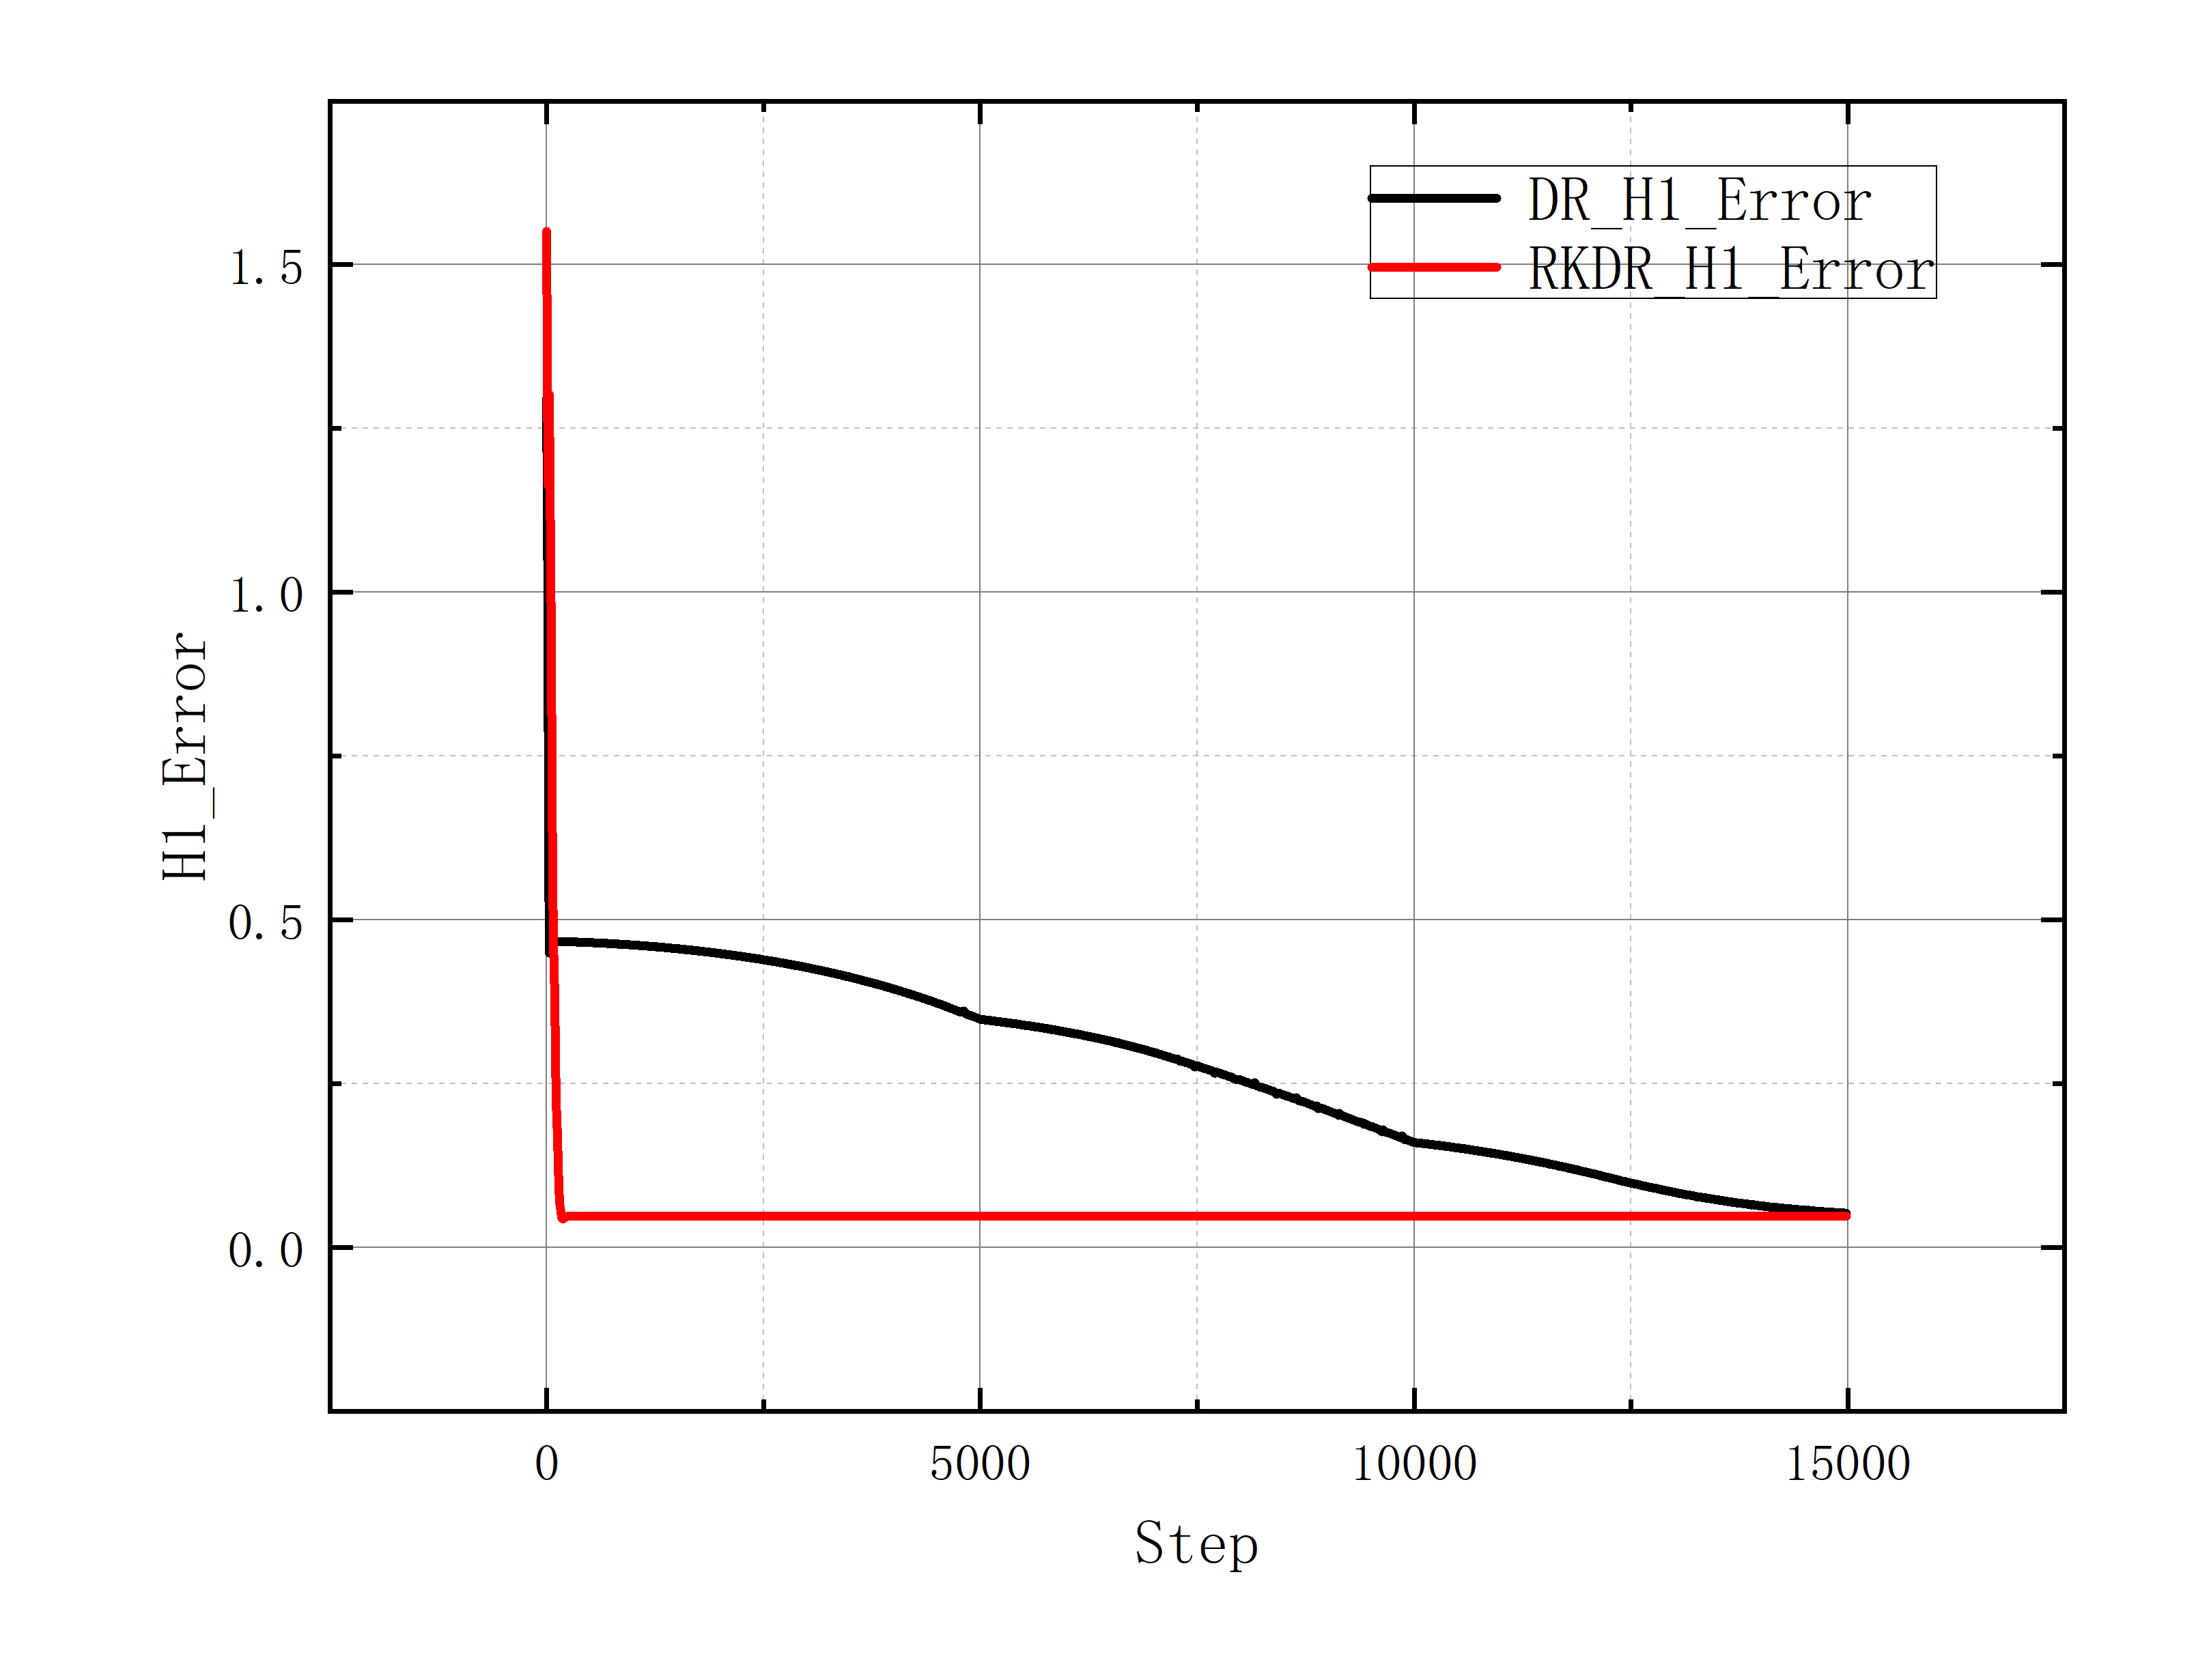
\includegraphics[width=\textwidth, height=6.5cm, keepaspectratio]{figures2/h1error.png}
        \caption{H1误差变化}
        \label{fig:h1_error}
    \end{subfigure}

    \caption{两算法误差对比}
    \label{fig:error_comparison1}
\end{figure}
\end{comment}
\begin{figure}[htbp]
    \centering
    \begin{subfigure}[b]{0.45\textwidth}
        \centering
        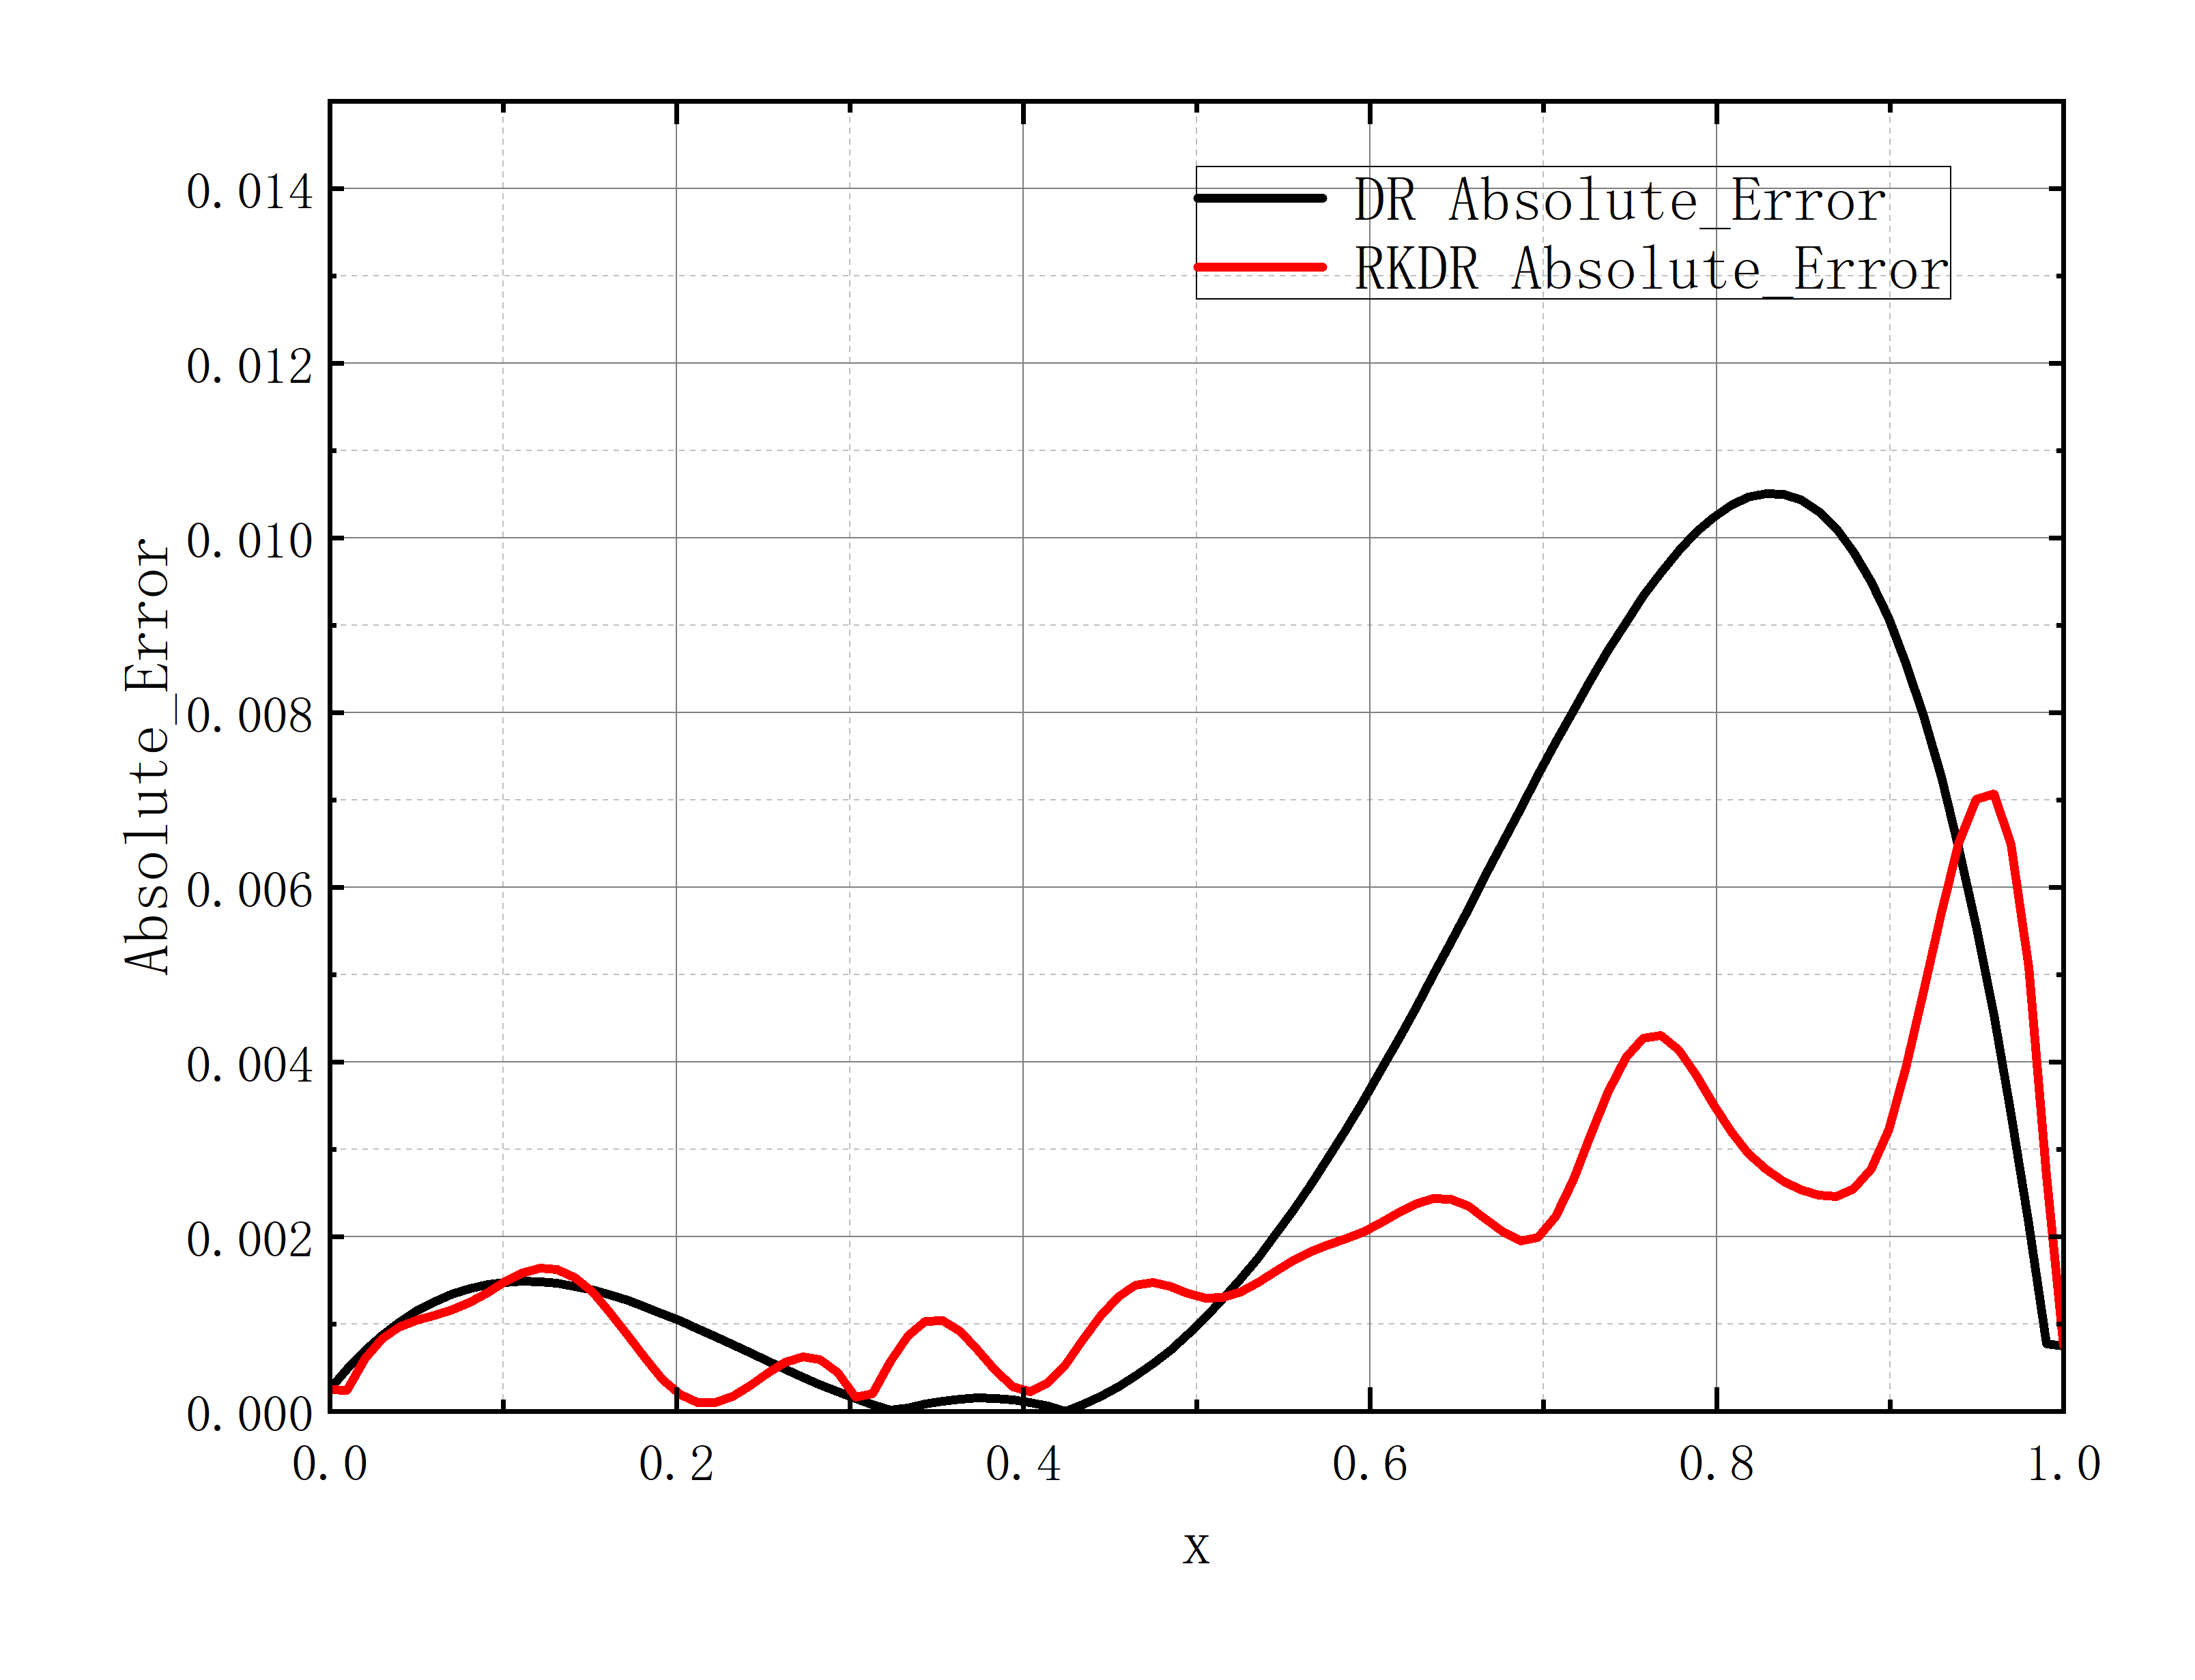
\includegraphics[width=\textwidth, height=5cm, keepaspectratio]{figures2/Abserror.png}
        \caption{绝对误差对比}
        \label{fig:abs_error}
    \end{subfigure}
    \hfill % 自动填充间距
    \begin{subfigure}[b]{0.45\textwidth}
        \centering
        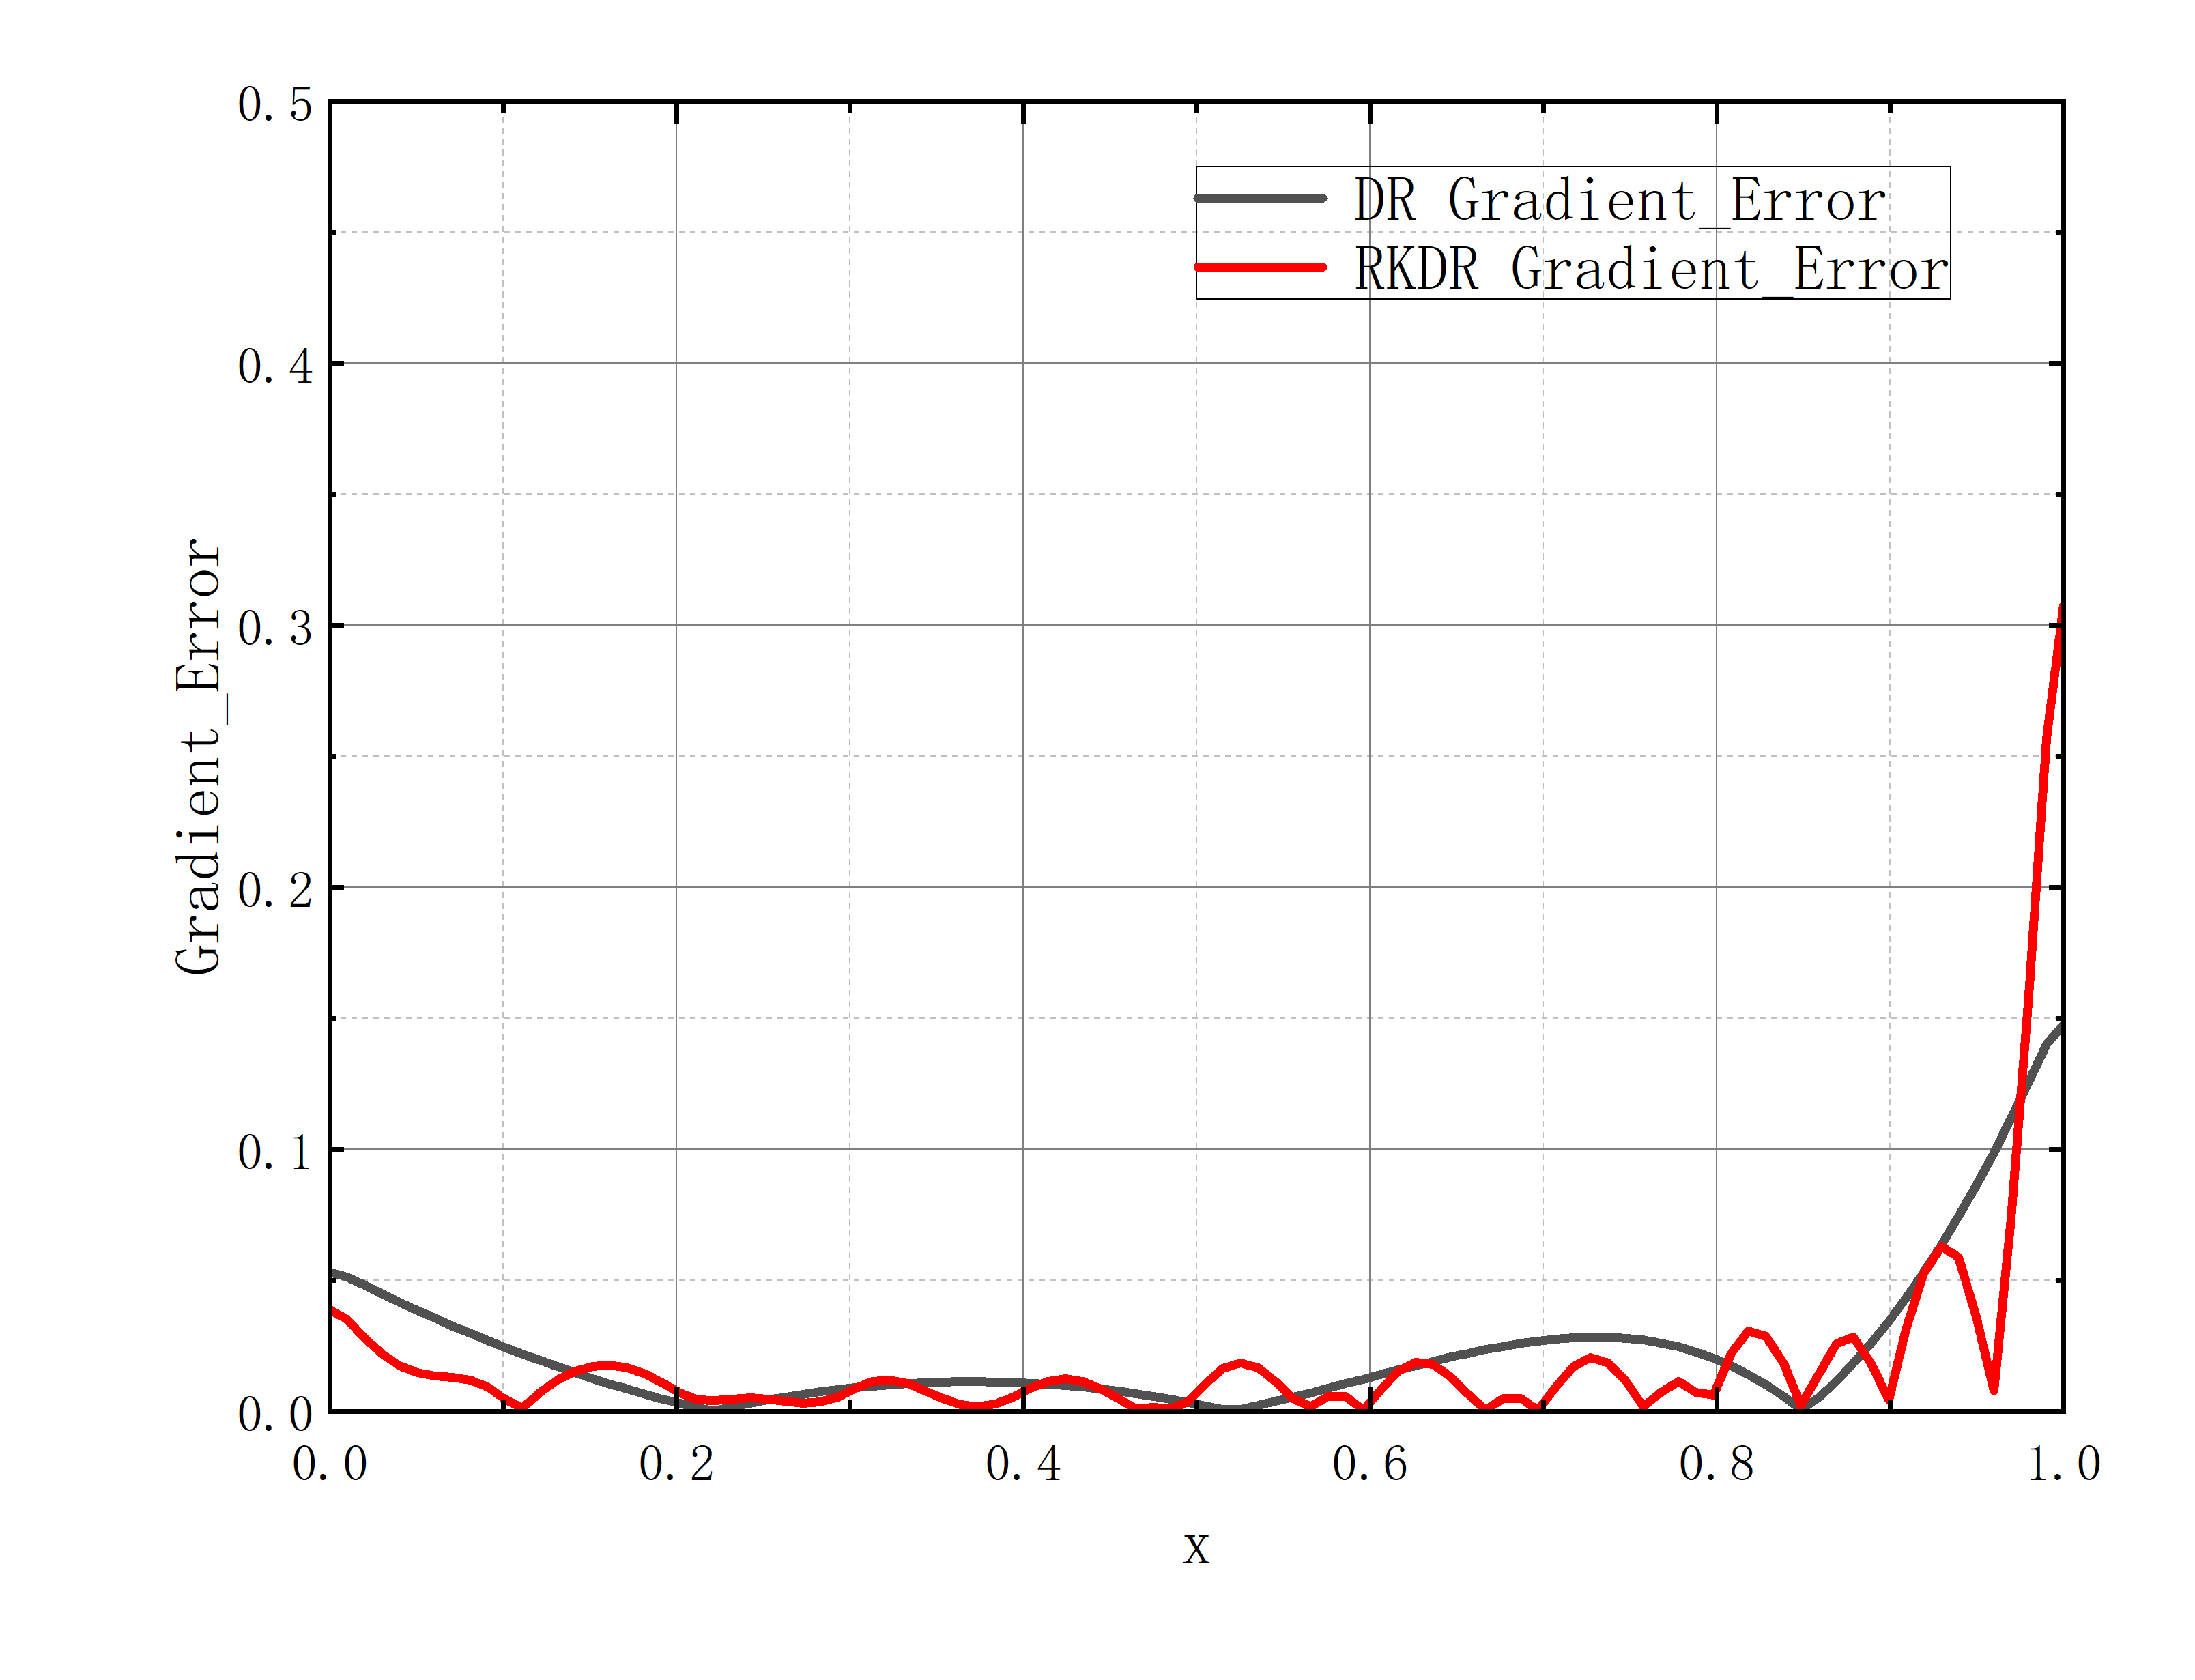
\includegraphics[width=\textwidth, height=5cm, keepaspectratio]{figures2/gradienterror.png}
        \caption{梯度误差对比}
        \label{fig:gradient_error}
    \end{subfigure}
    \caption{两算法的绝对误差和梯度误差对比}
    \label{fig:abs_gradient_error}
\end{figure}


\begin{figure}[htbp]
    \centering
    \begin{subfigure}[b]{0.45\textwidth}
        \centering
        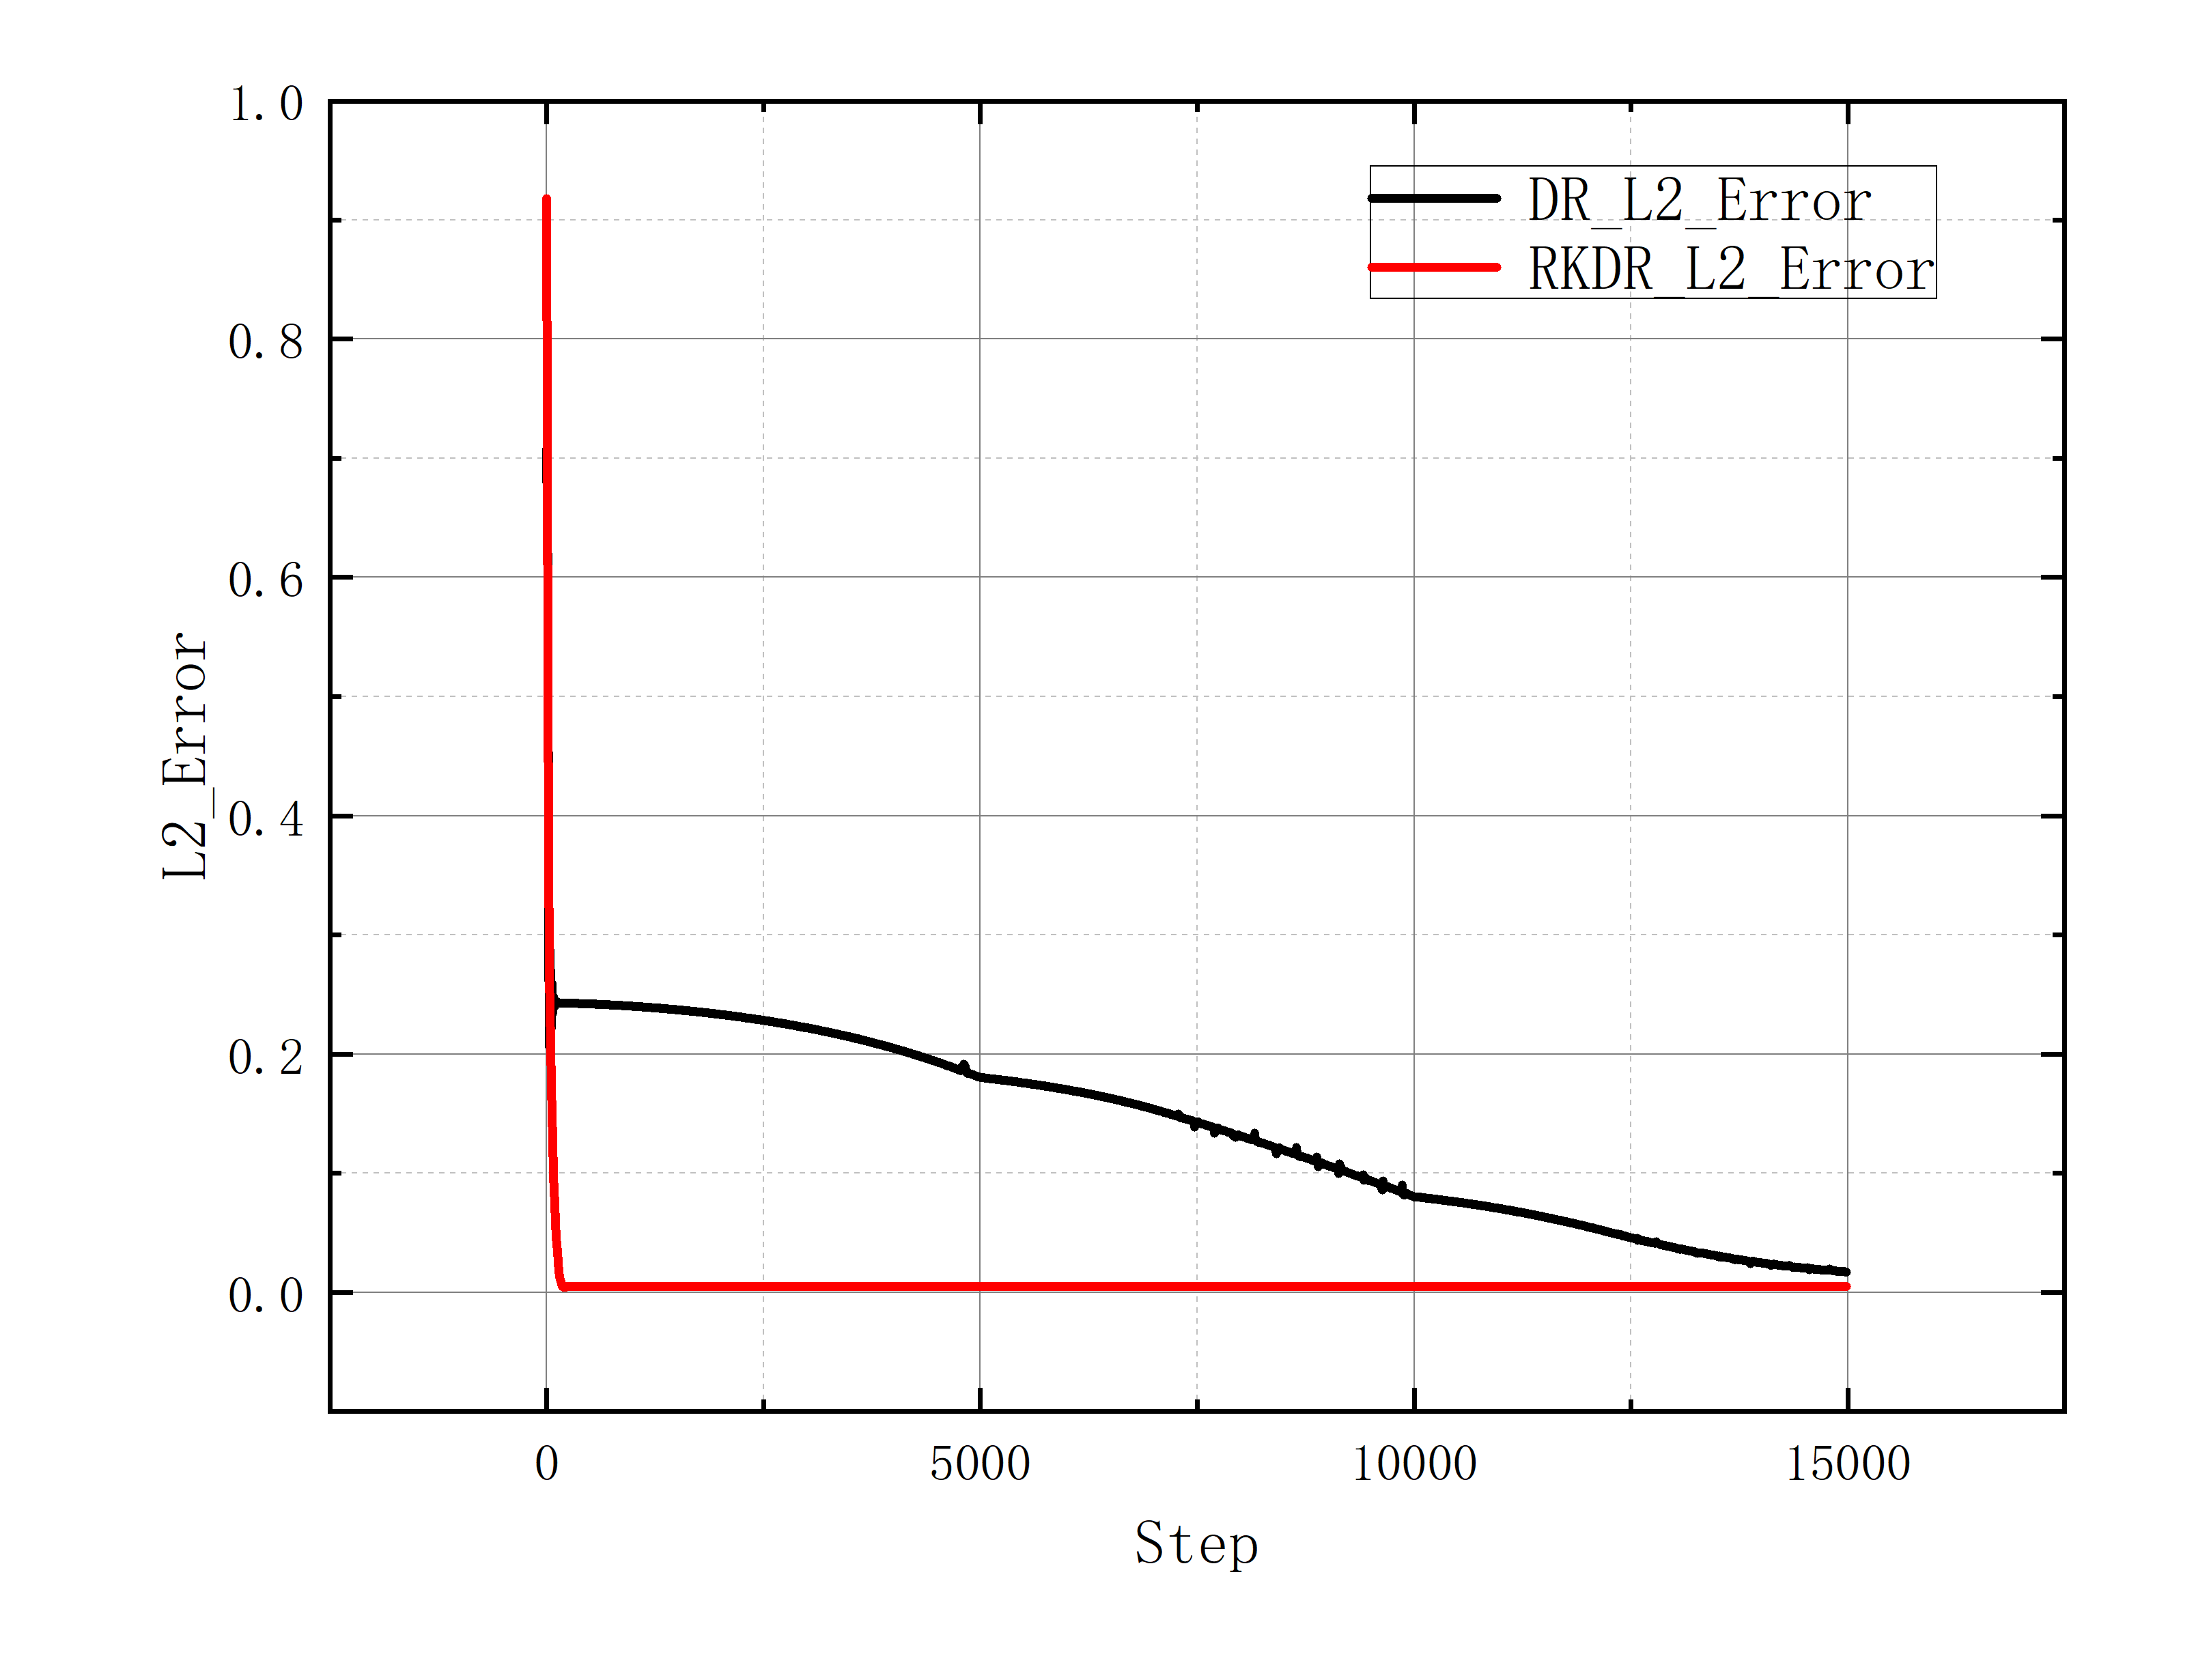
\includegraphics[width=\textwidth, height=5cm, keepaspectratio]{figures2/l2error.png}
        \caption{L2误差变化}
        \label{fig:l2_error}
    \end{subfigure}
    \hfill % 自动填充间距
    \begin{subfigure}[b]{0.45\textwidth}
        \centering
        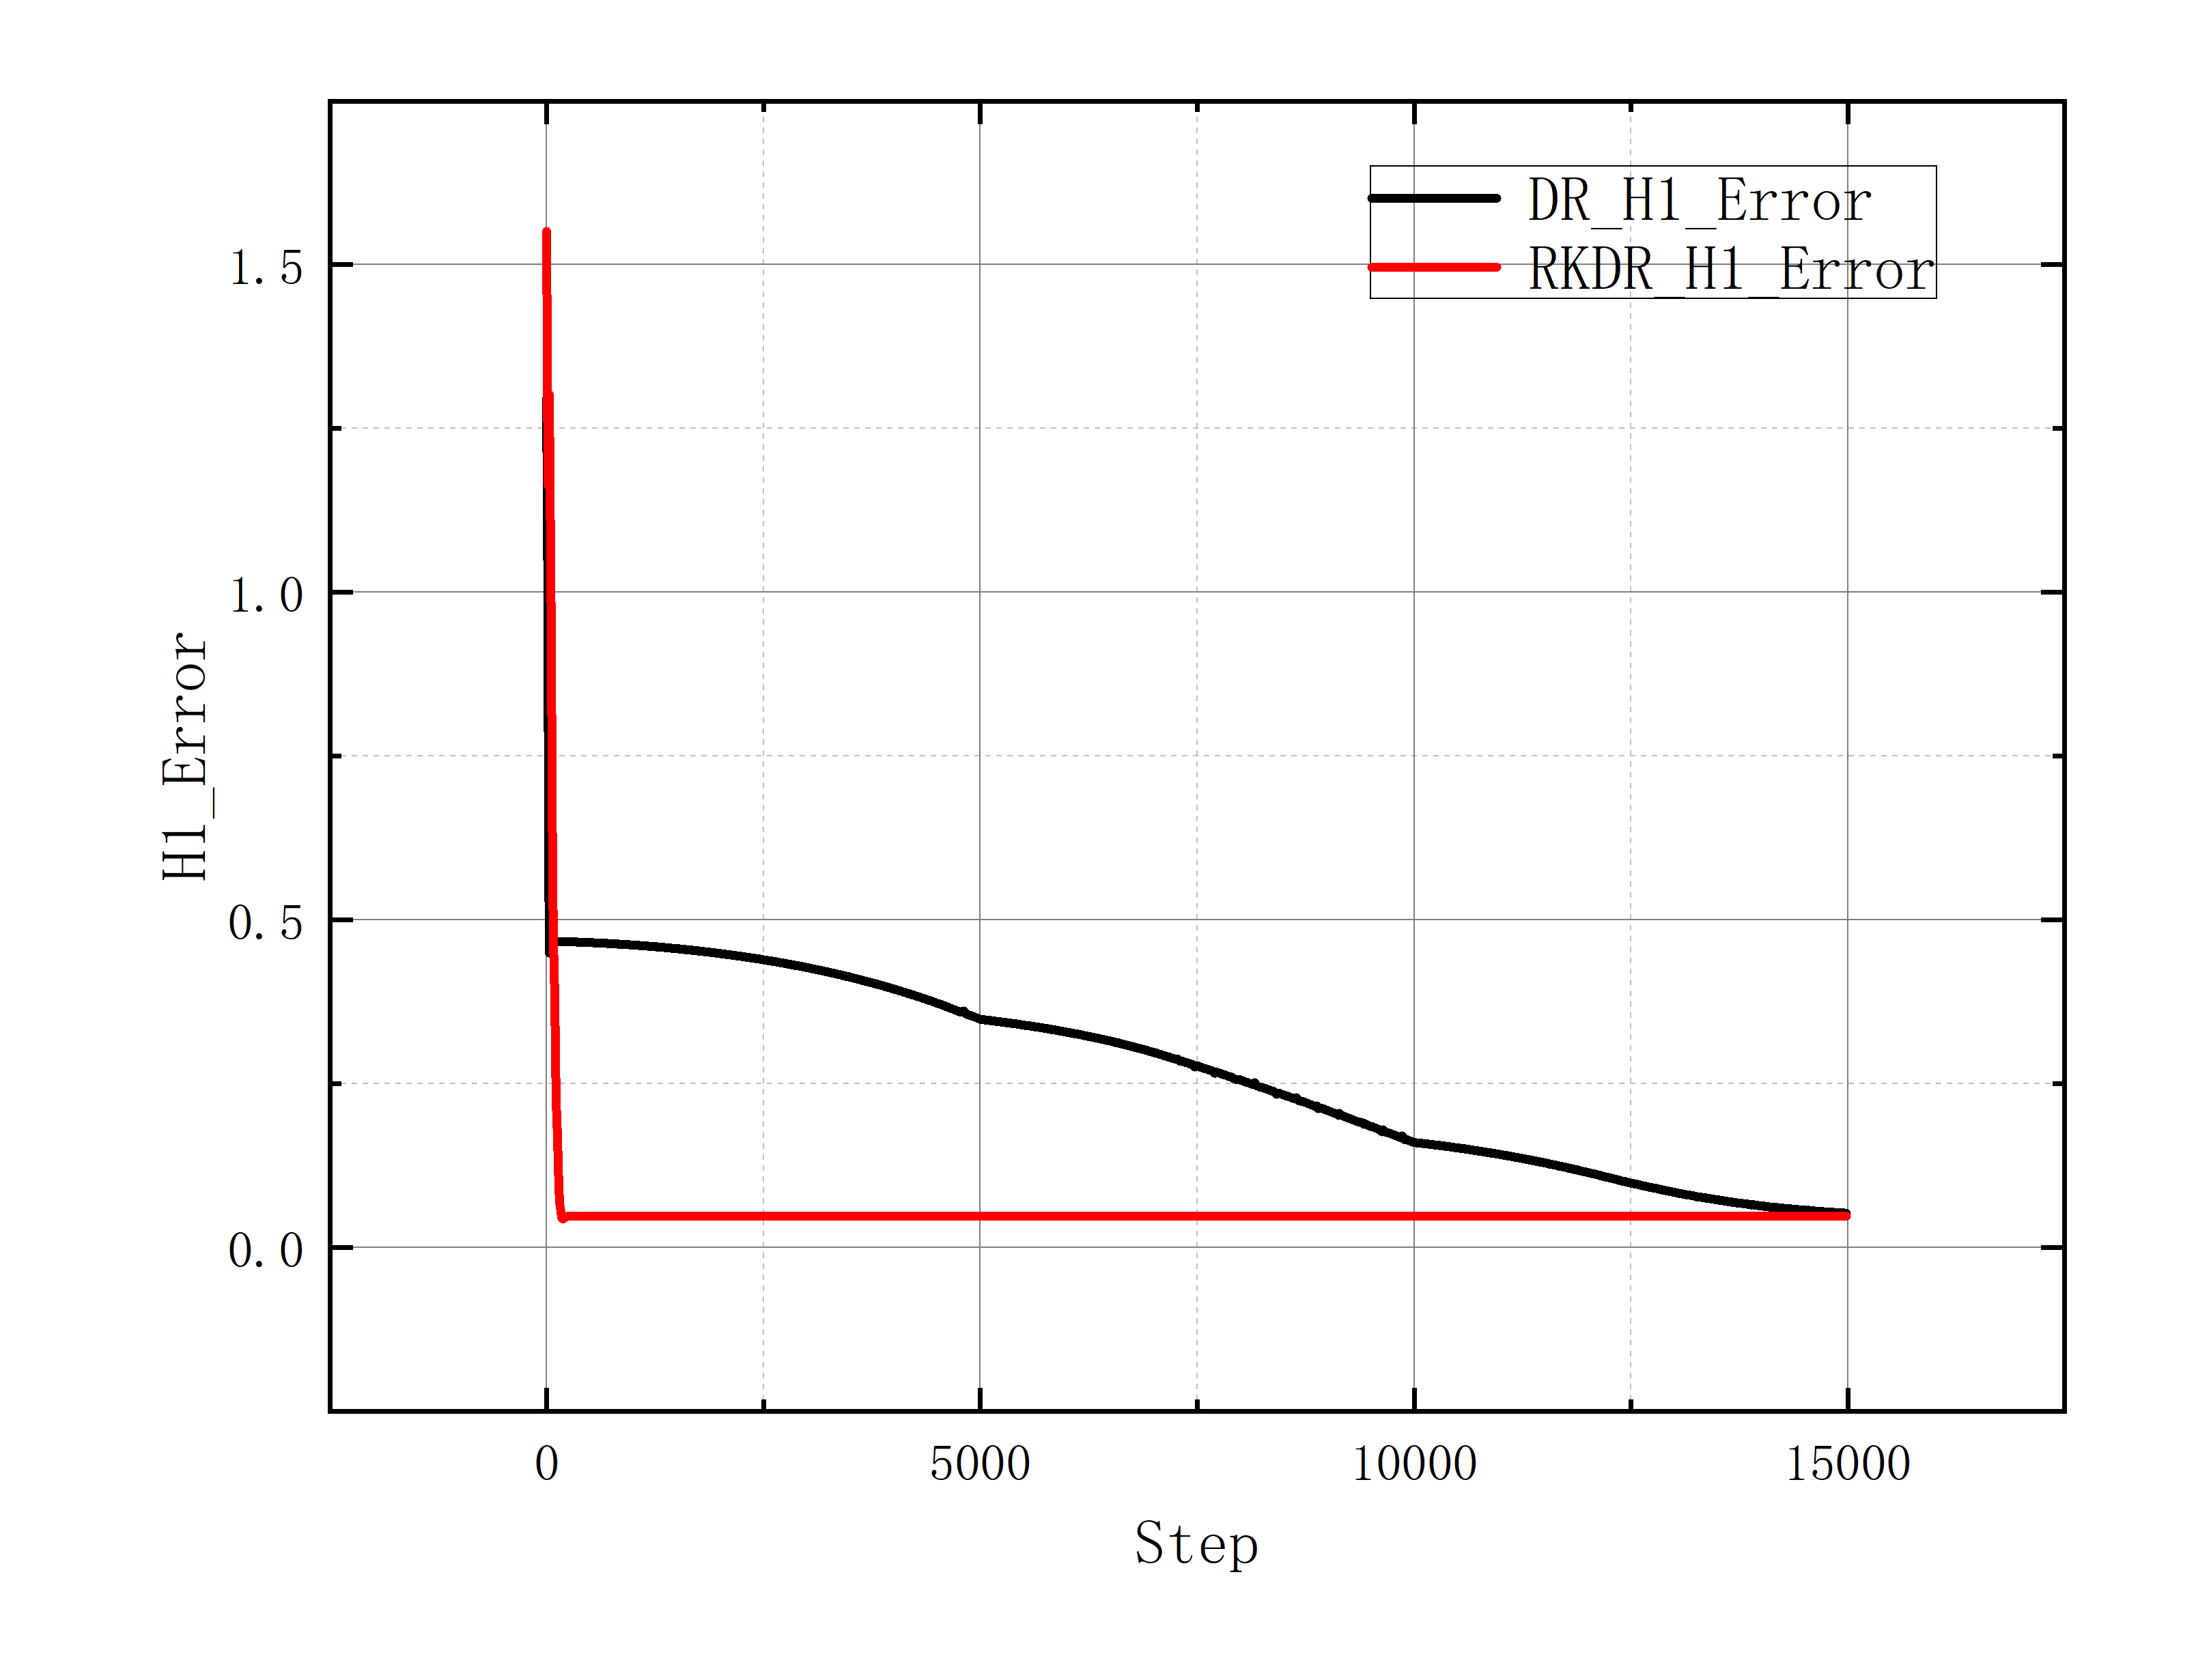
\includegraphics[width=\textwidth, height=5cm, keepaspectratio]{figures2/h1error.png}
        \caption{H1误差变化}
        \label{fig:h1_error}
    \end{subfigure}
    \caption{两算法的L2误差和H1误差变化}
    \label{fig:l2_h1_error}
\end{figure}

\begin{figure}[htbp]
    \centering
    \begin{subfigure}[b]{0.48\textwidth}
        \centering
        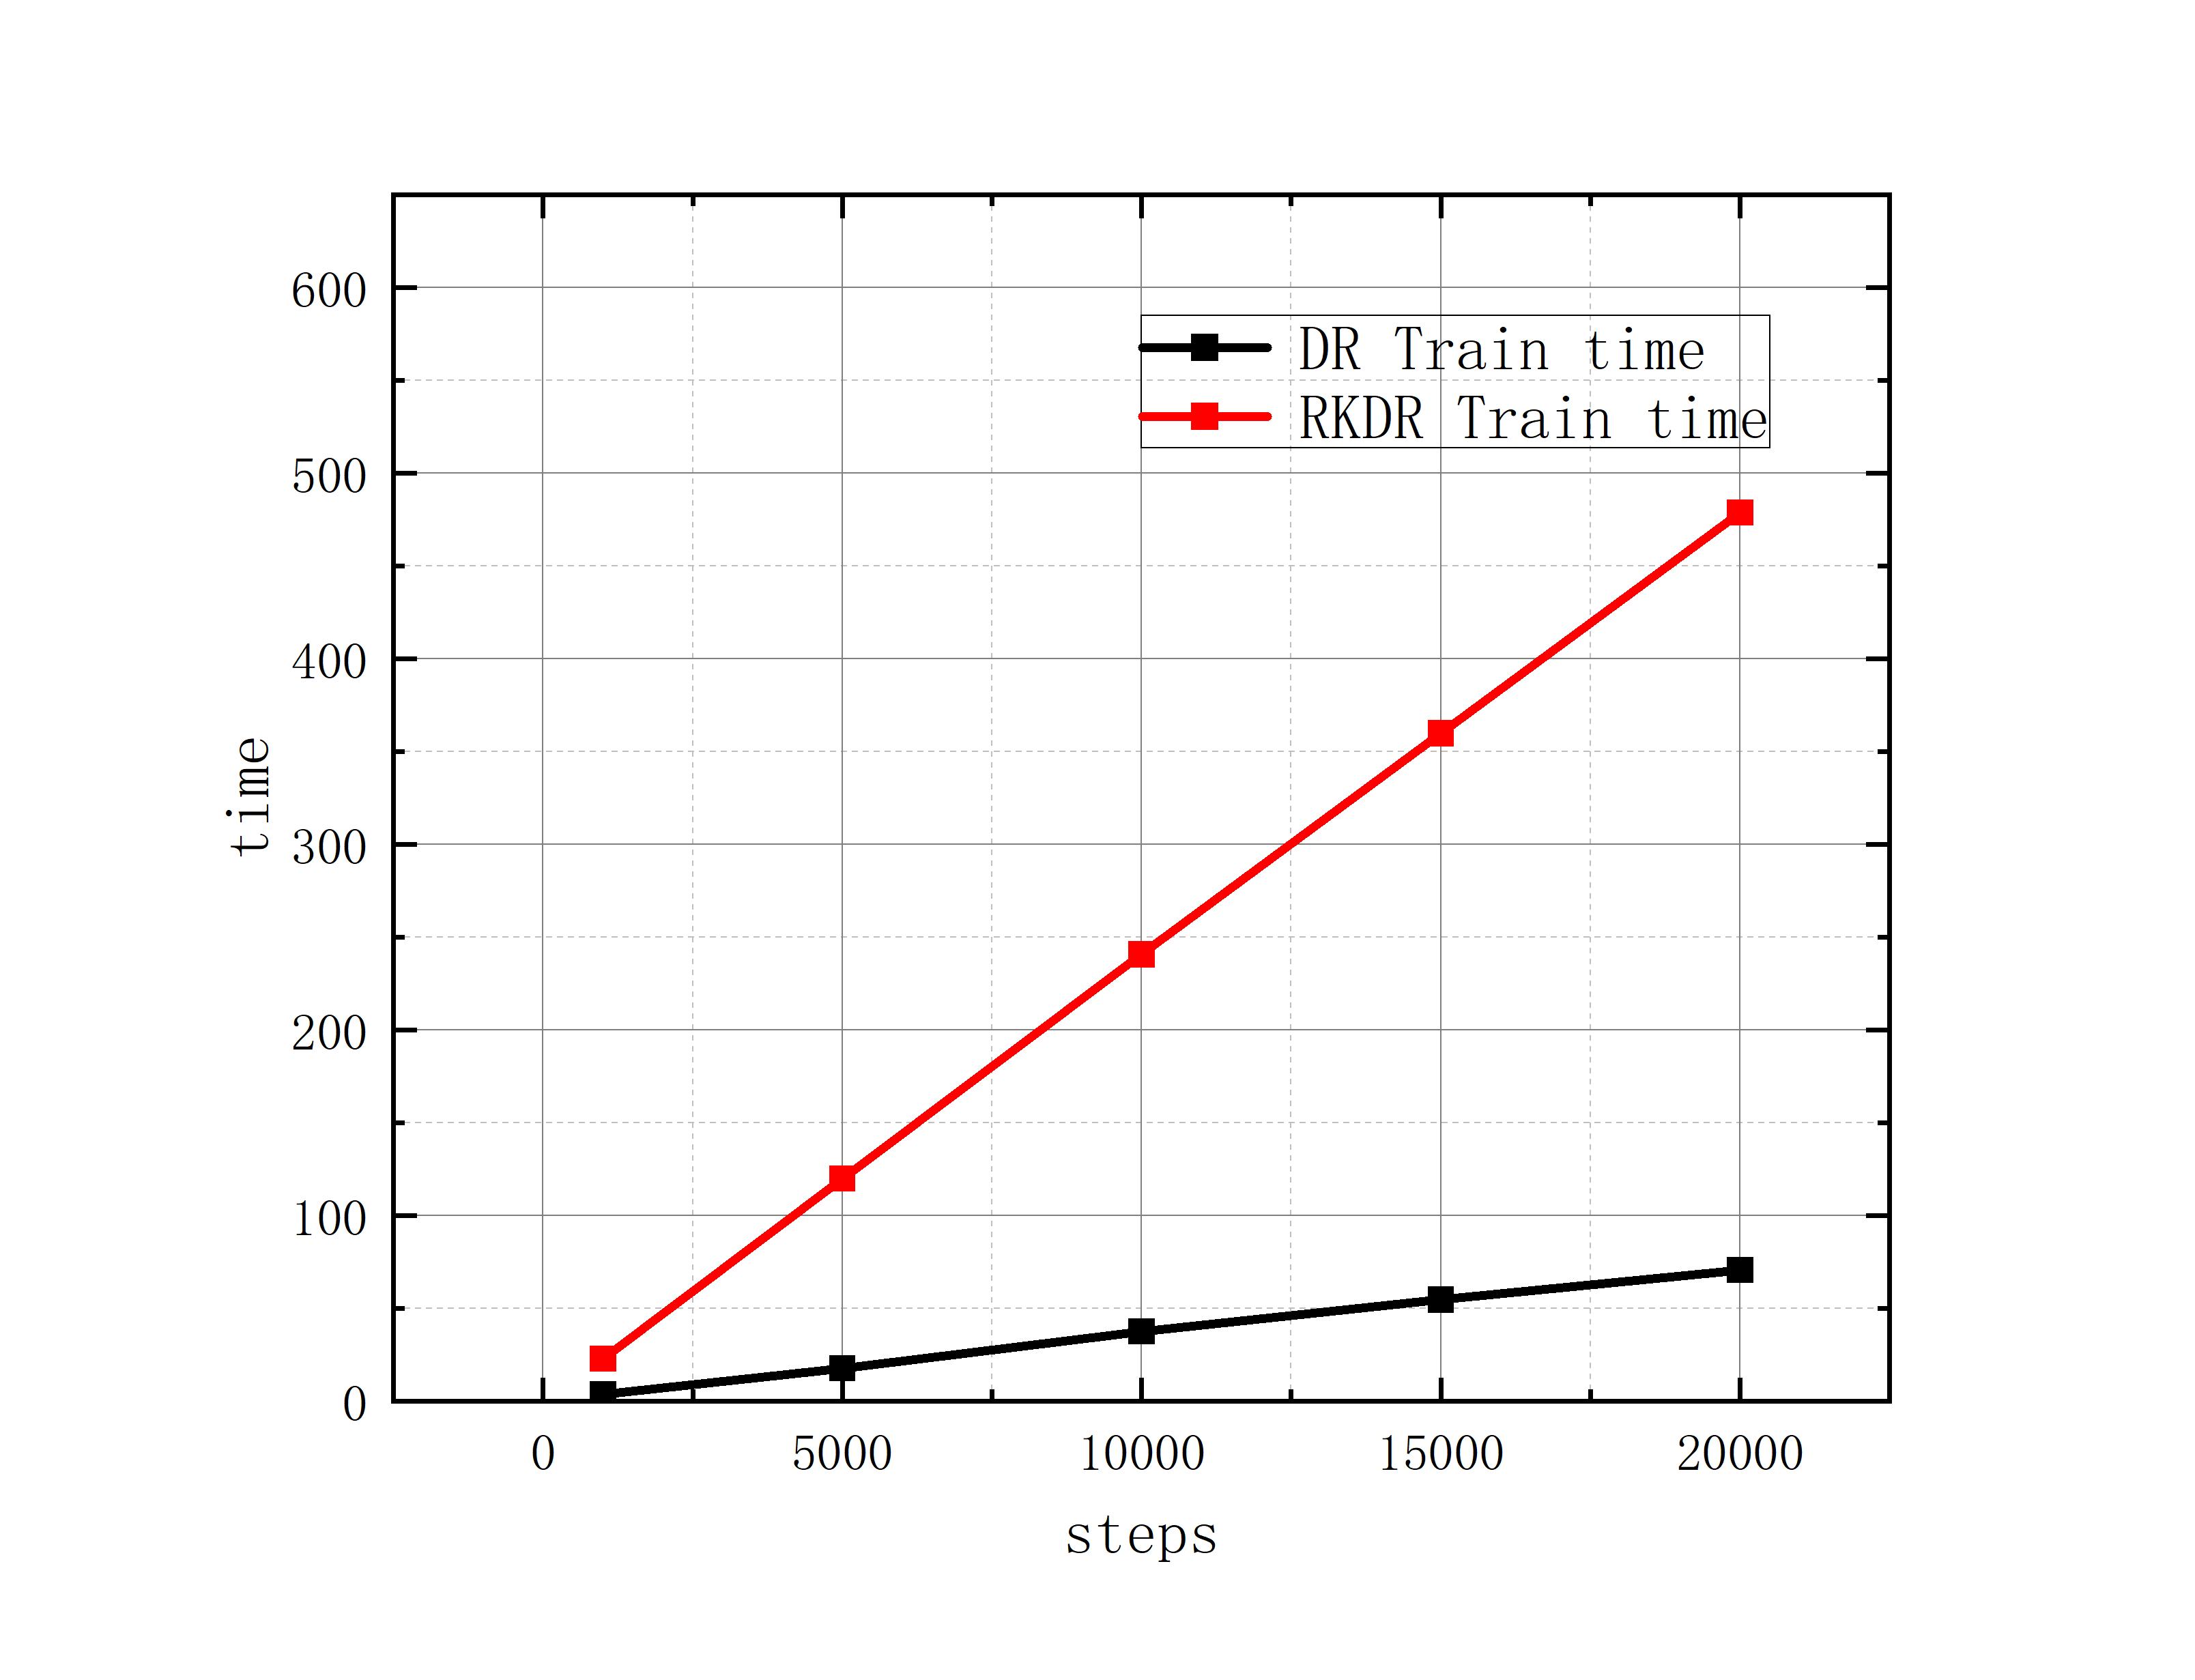
\includegraphics[width=\textwidth, height=6.5cm, keepaspectratio]{figures2/traintime2.png}
        \caption{训练时间对比}
        \label{fig:100stepsloss}
    \end{subfigure}
    \hspace{0.5em} % 减小水平间距
    \begin{subfigure}[b]{0.48\textwidth}
        \centering
        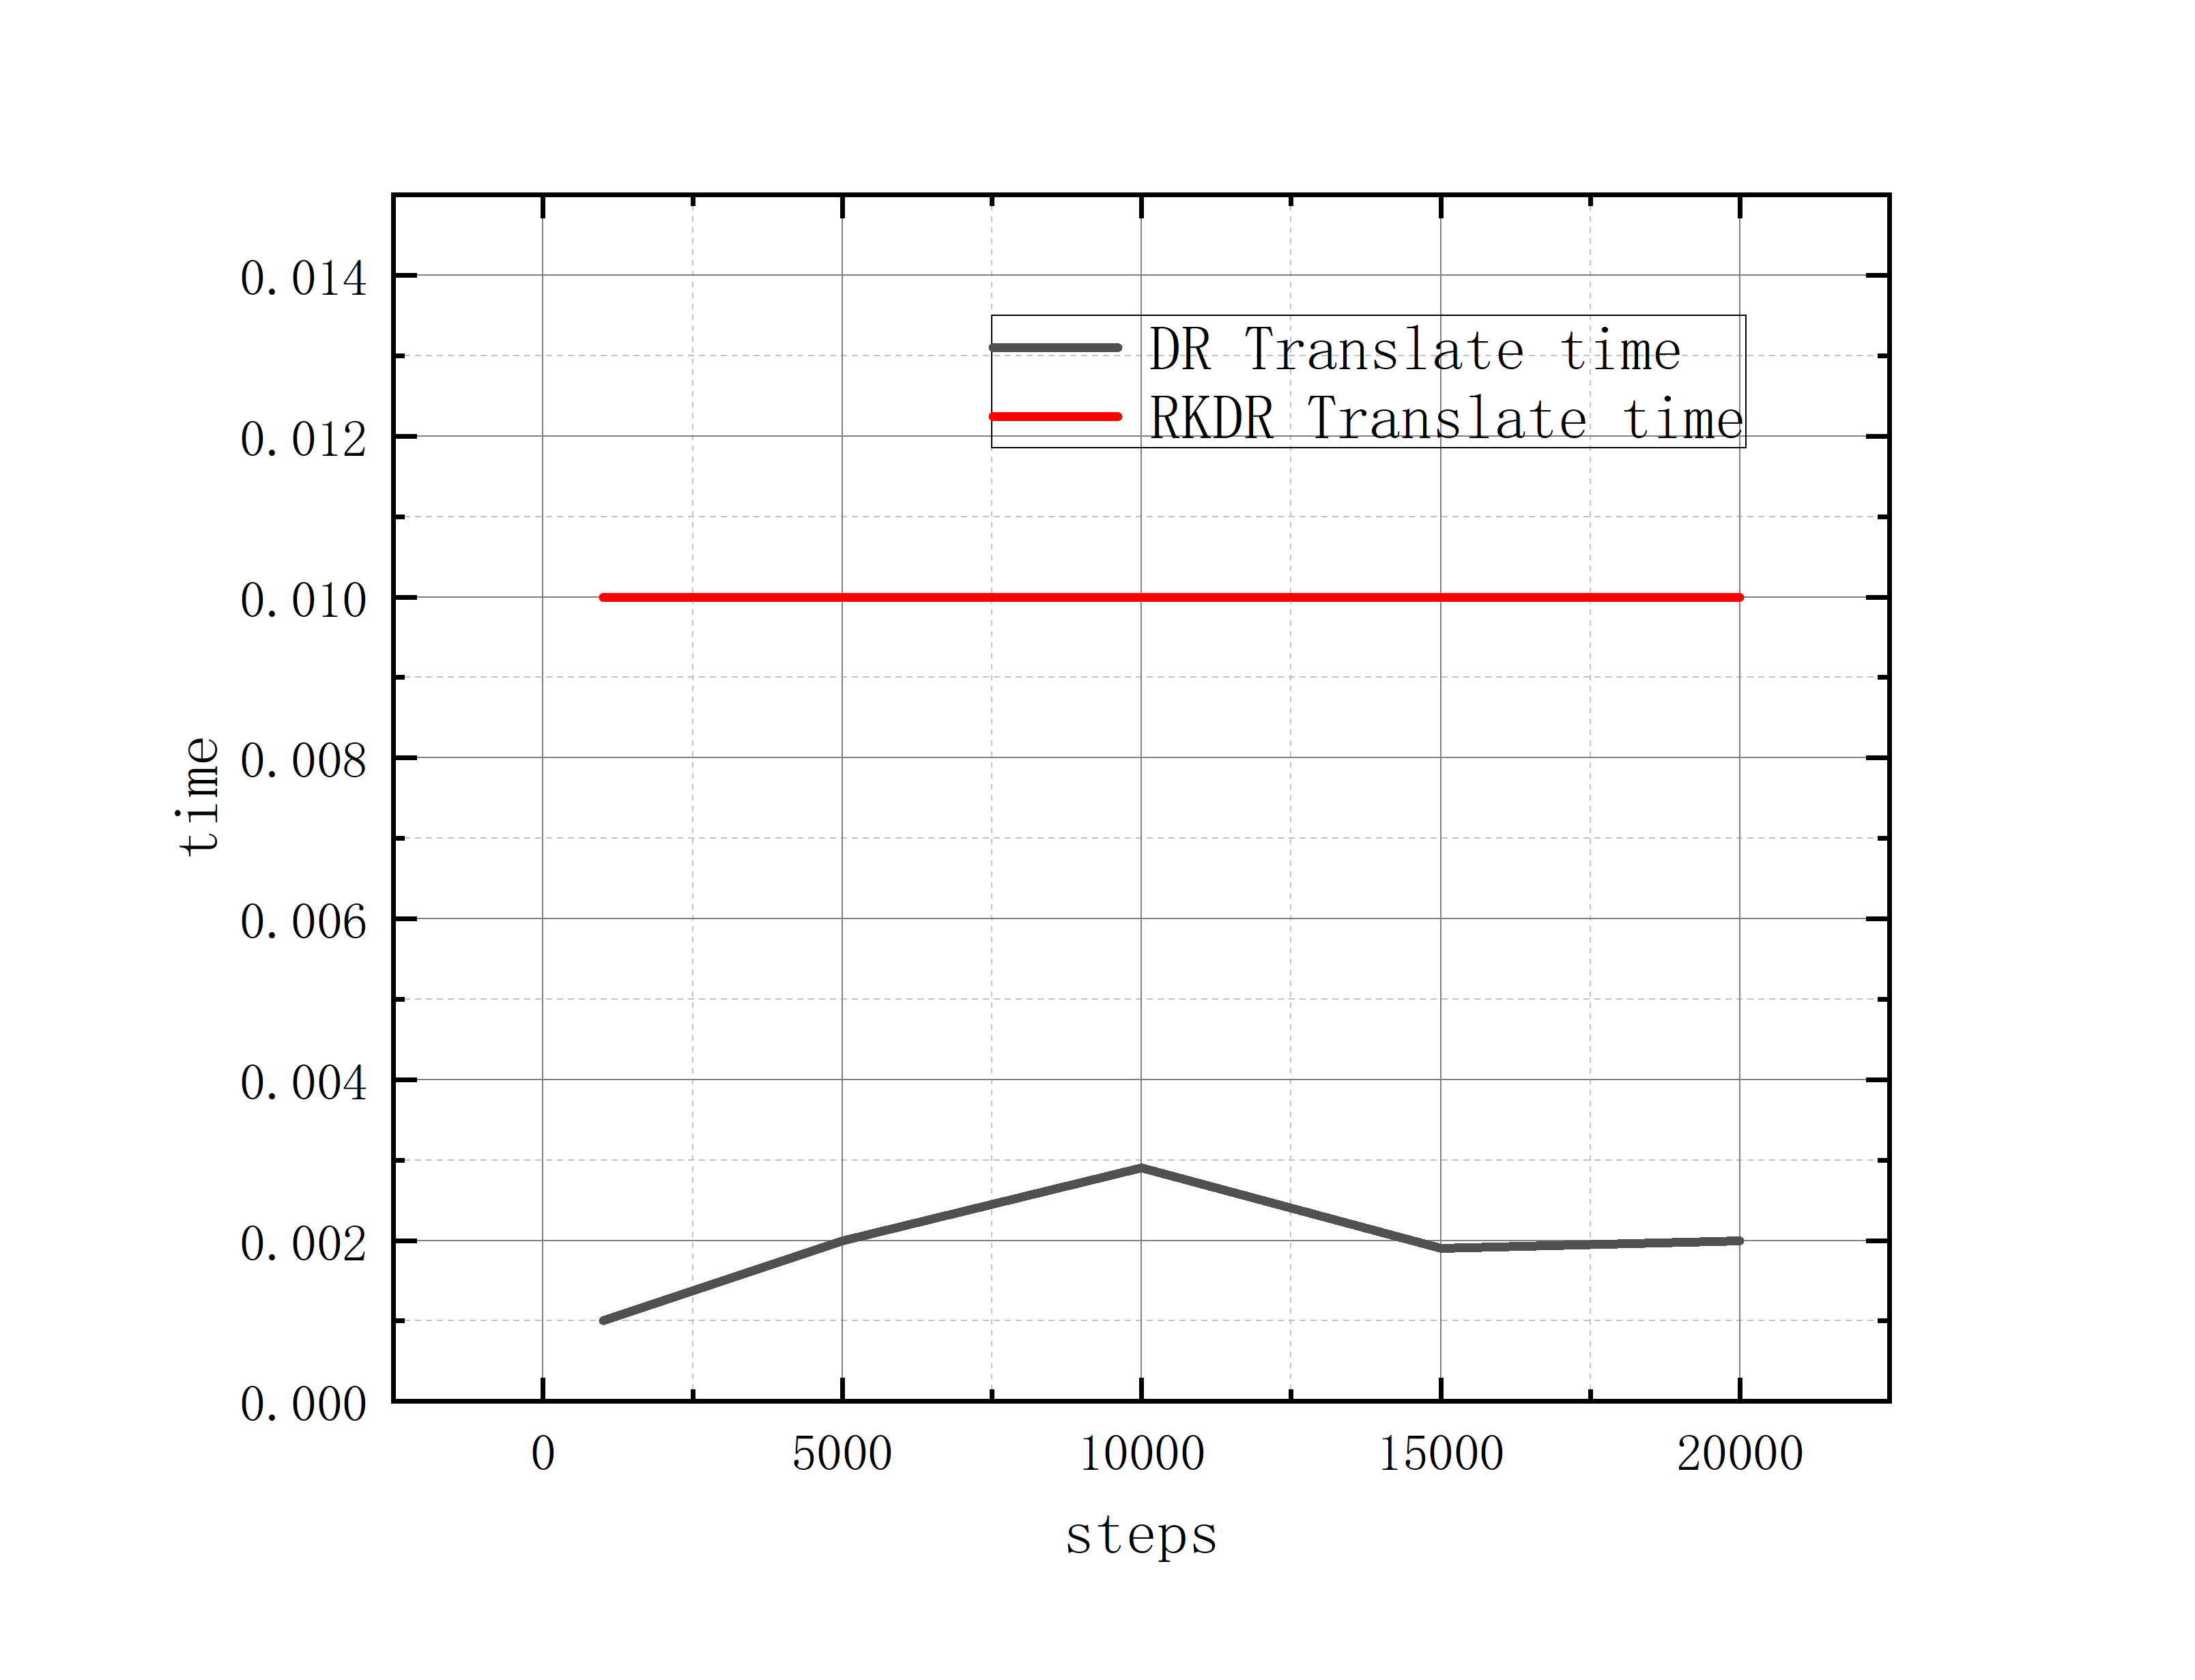
\includegraphics[width=\textwidth, height=6.5cm, keepaspectratio]{figures2/translatetime.png}
        \caption{计算时间对比}
        \label{fig:allstepsloss}
    \end{subfigure}

    \caption{时间对比}
    \label{fig:time}
\end{figure}


对于 DR 方法，其训练时间随步数增加呈现较为平缓的线性增长趋势。在 20000 步时，DR 方法的训练时间约为 100 秒，表明其训练过程较为稳定，整体耗时较短。相比之下，由于再生核增强引入了额外的计算复杂度，RKDR 方法的训练时间增长速度显著更快，在 20000 步时达到约 500 秒。这表明 RKDR 方法在训练过程中的单步计算成本高于 DR 方法。

然而，结合收敛数据，DR 方法需要 13210 步（51.09 秒）才能收敛，而 RKDR 方法仅需 670 步（14.47 秒）。尽管 RKDR 方法的单步训练时间较高，但其收敛速度远快于 DR 方法。RKDR 方法的实际训练用时远低于 DR 方法，这表明 RKDR 方法通过更快的收敛速度，显著降低了总体训练时间，展现了更高的计算效率。

从理论角度看，RKDR 方法通过引入再生核，增强了神经网络的逼近能力，使其能够更快地逼近最优解，从而减少了所需的训练步数。再生核的数学完备性不仅提高了逼近精度（见之前的误差分析），还优化了训练过程，使 RKDR 方法在计算效率上具有显著优势。

\begin{figure}[htbp]
    \centering
    \begin{subfigure}[b]{0.48\textwidth}
        \centering
        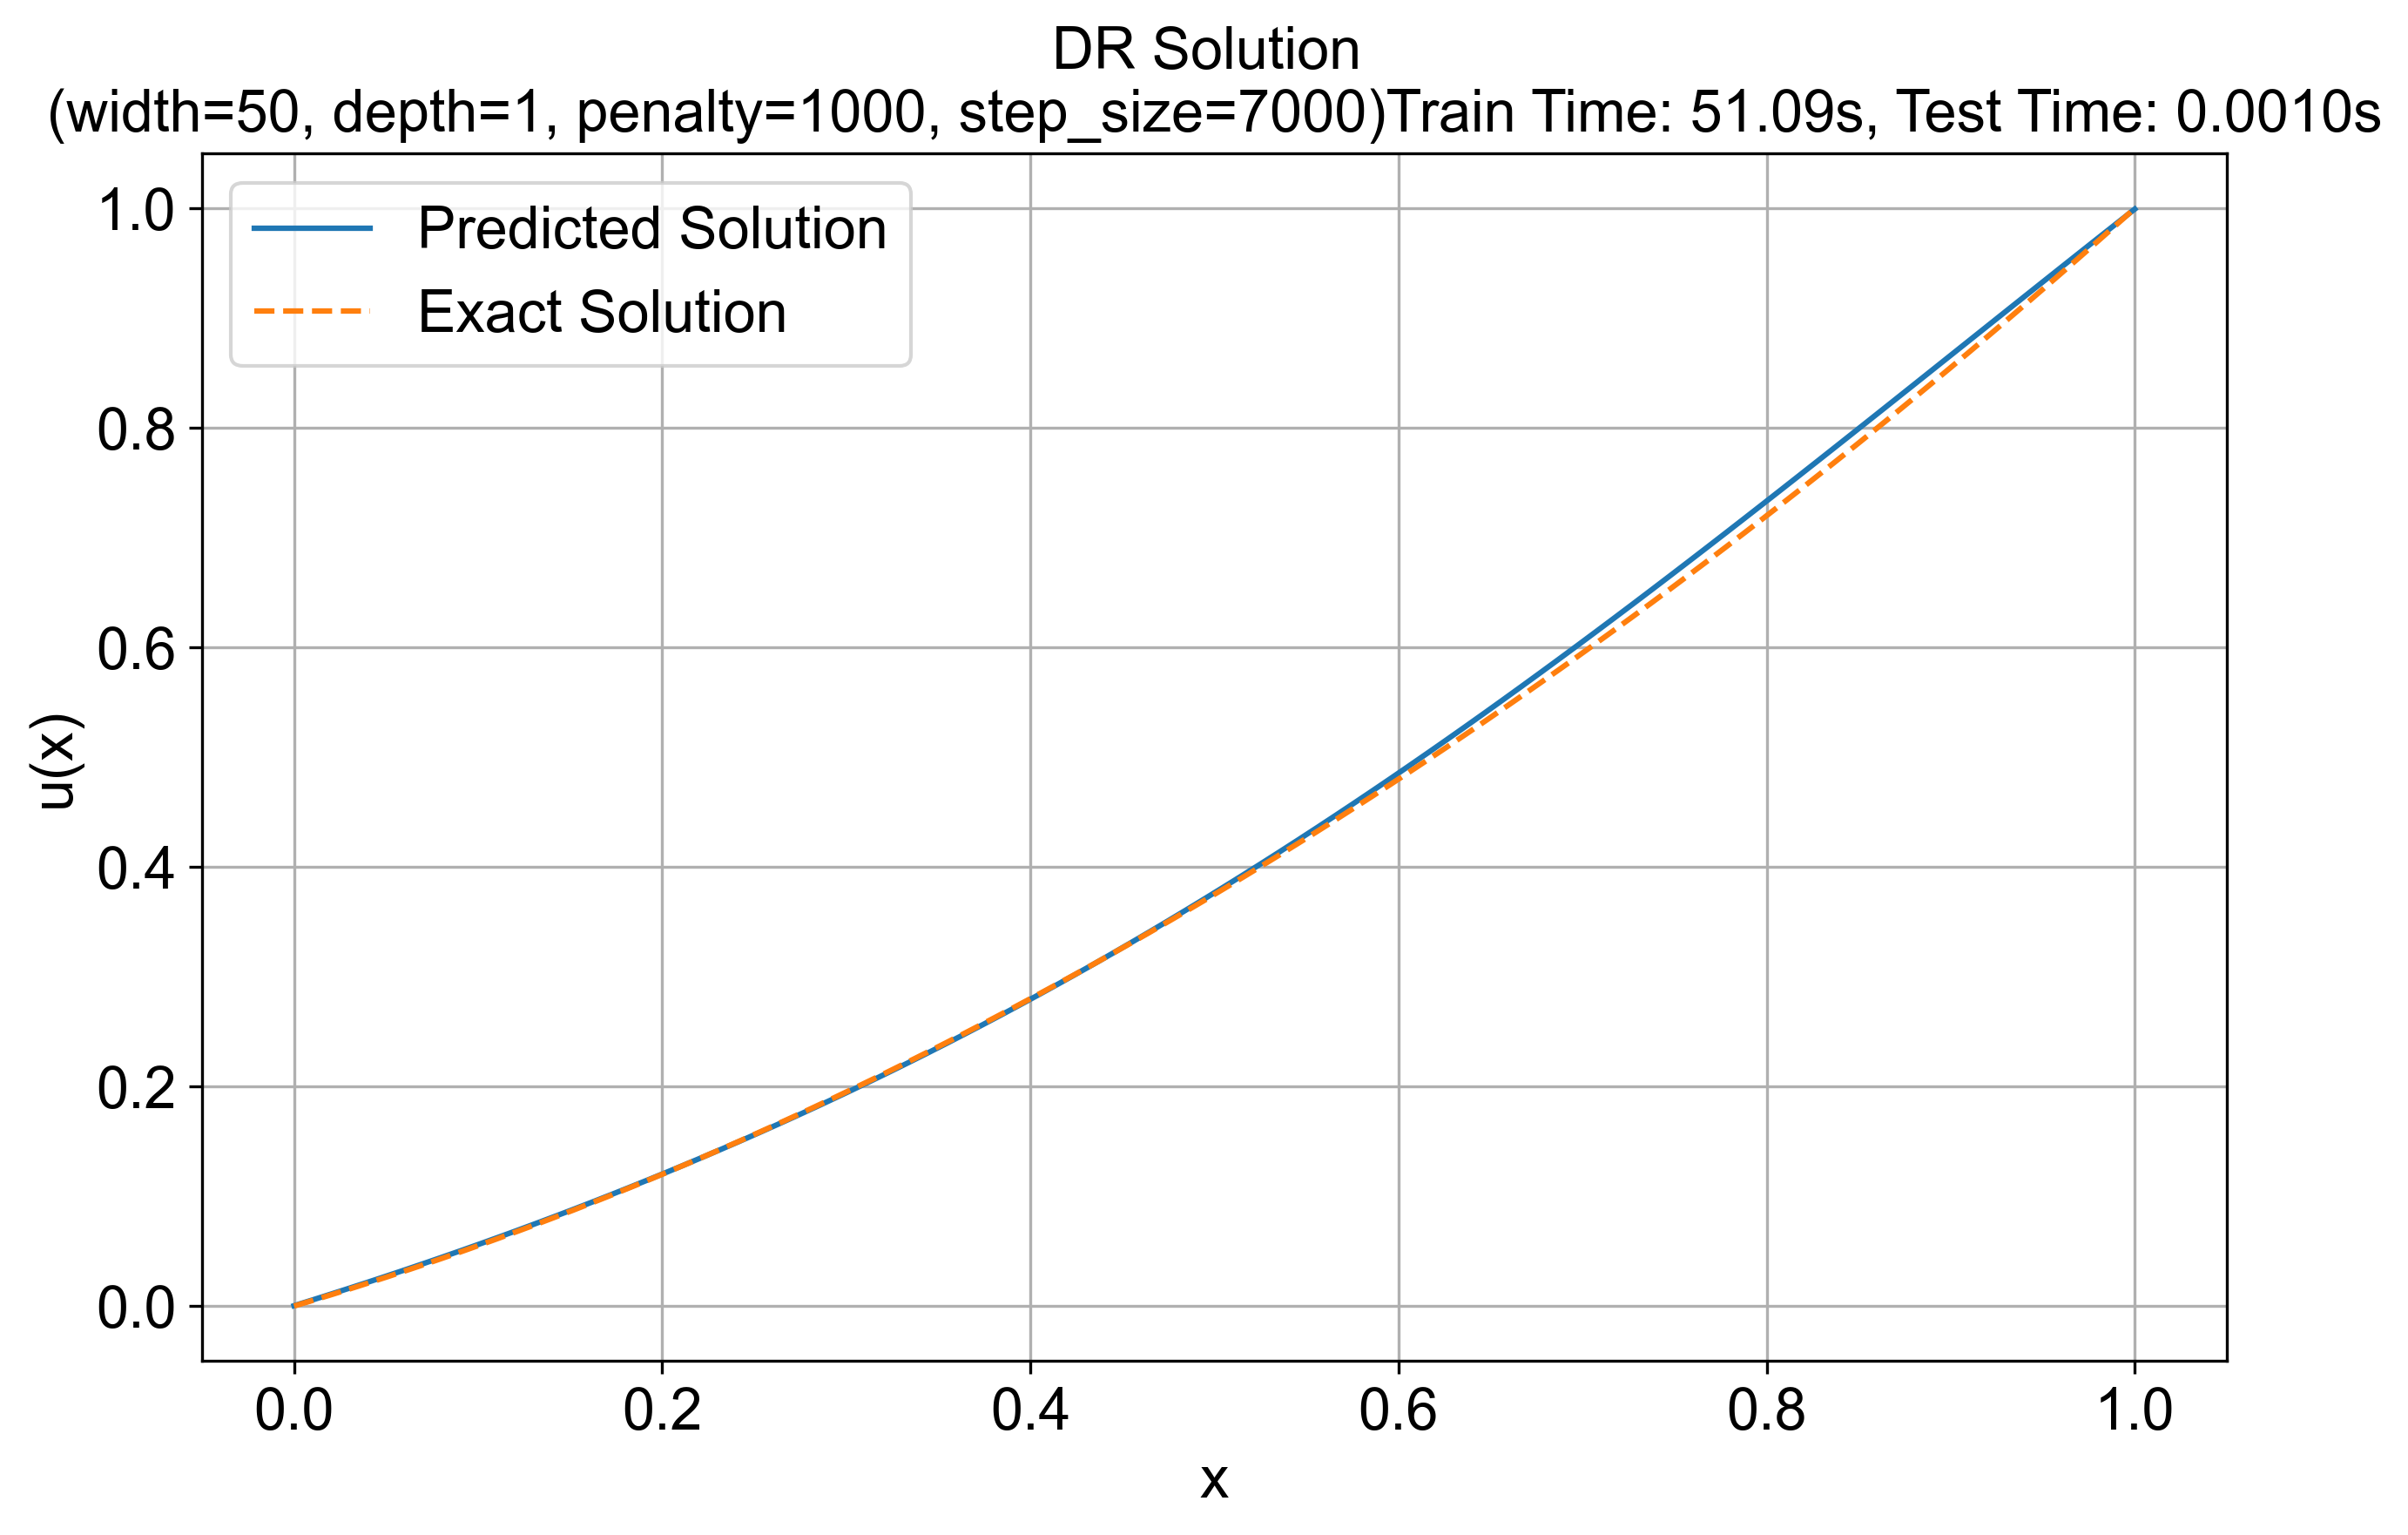
\includegraphics[width=\textwidth, height=6.5cm, keepaspectratio]{figures2/3-7-1.png}
        \caption{DR方法收敛预测情况}
        \label{fig:allstepsloss}
    \end{subfigure}
    \hspace{0.5em} % 减小水平间距
    \begin{subfigure}[b]{0.48\textwidth}
        \centering
        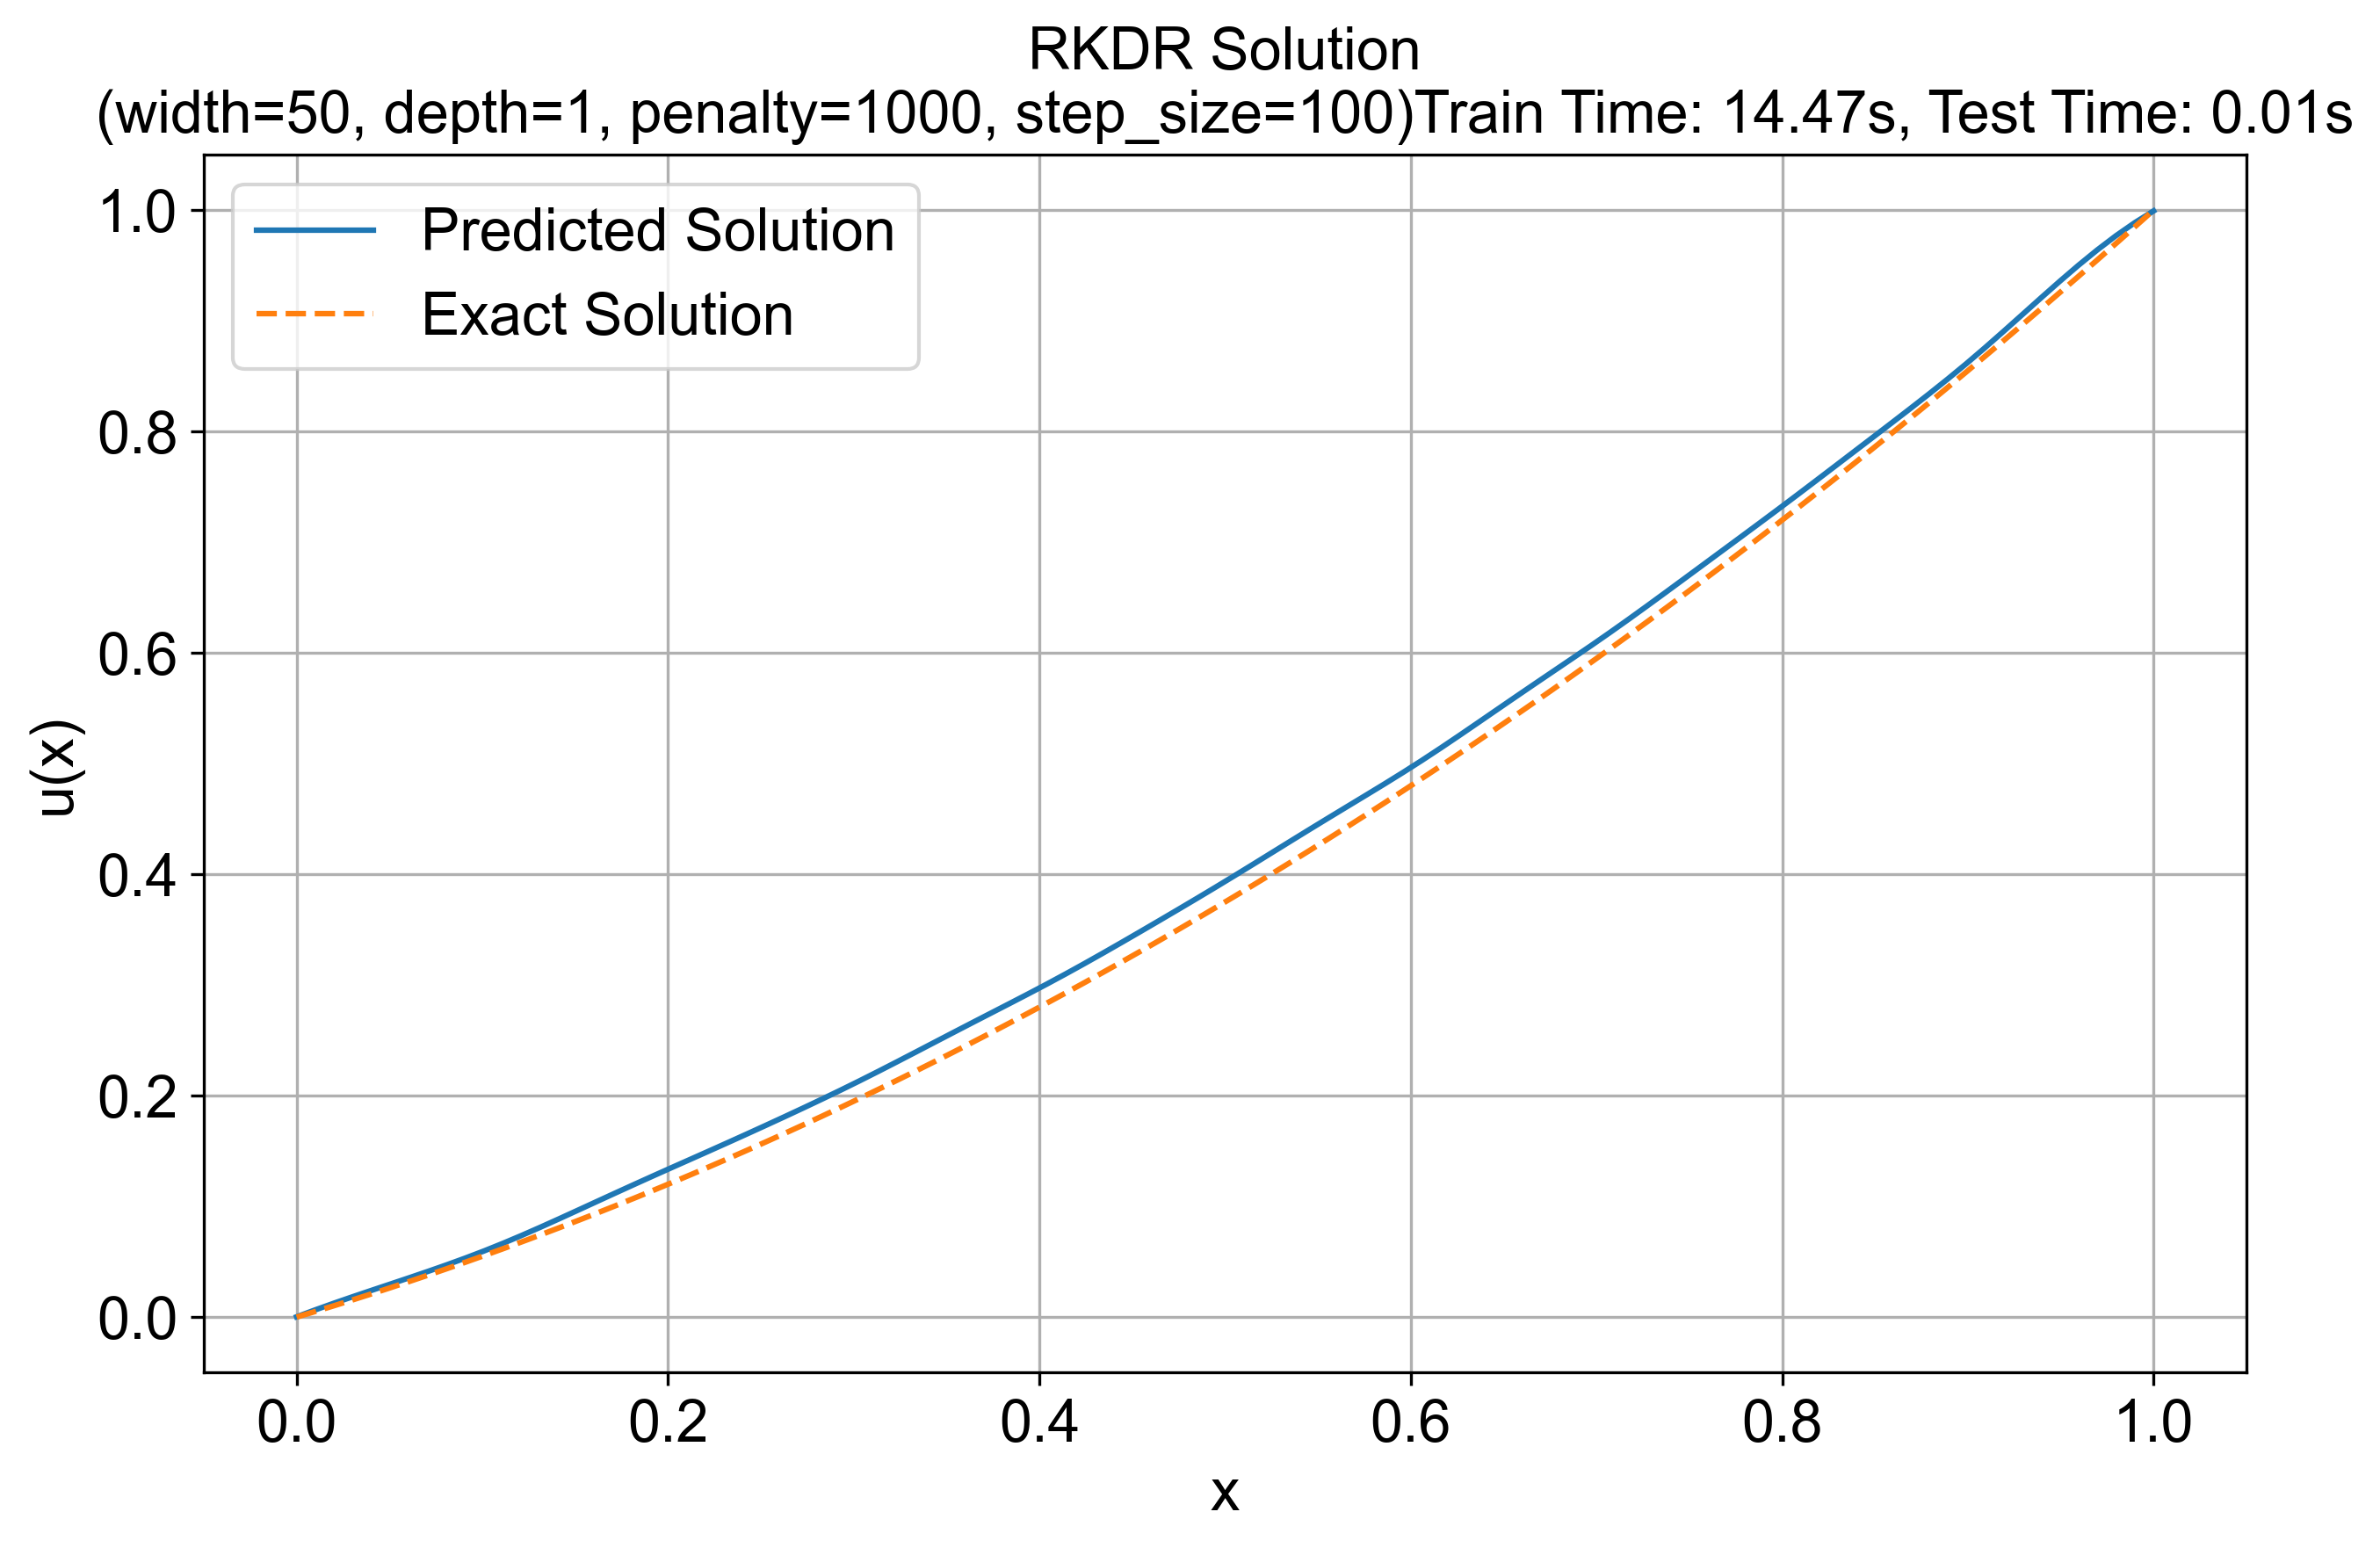
\includegraphics[width=\textwidth, height=6.5cm, keepaspectratio]{figures2/5-5-1.png}
        \caption{RKDR方法收敛预测情况}
        \label{fig:allstepsloss}
    \end{subfigure}
     \caption{收敛时间对比}
    \label{fig:shouliantime}
\end{figure}

\chapter{结论}


本文提出的再生核增强深度 里兹 法（RK-Deep里兹）融合深度学习与无网格方法，基于 里兹 变分原理，通过再生核增强提升偏微分方程求解的精度与效率。方法在深度神经网络框架下引入再生核近似，针对一维问题实现显著的 $L^2$ 误差降低，展现出较高的推理效率与应用潜力。

首先，深度 里兹 方法以里兹方法为基础，通过预定义基函数近似位移场，而深度 里兹 方法利用神经网络替代试函数，验证了其数值有效性。其次，伽辽金无网格法（RKPM）从弱形式出发，通过无网格离散化构造形状函数，结合拉格朗日乘子法强制边界条件并采用高斯积分法近似积分，显示出较好的导数拟合能力。最后，本文主要实现再生核近似增强深度 里兹 法，通过再生核近似机制增强局部解表达能力，验证了方法的优越性。

RKDR 方法在 700 步内（14.47s）即达到完全收敛，而DR 方法需要 12000 步（51.09s）才能稳定，表明 DR 方法在收敛速度上显著优于 RKDR 方法，尽管增强方法性能优于原始深度 里兹 方法，但 H1 误差中的梯度误差仍较高。

RKDR方法在 $L^2$ 误差上优于 RKPM 和 Deep里兹，在 $H^1$ 误差上低于 Deep里兹 但高于 RKPM，中间区域精度更高，导数误差波动较大，边界处需优化。训练时间较长但计算时间远低于 RKPM，验证了推理效率优势，为复杂偏微分方程求解提供了高效工具。增强深度 里兹 方法通过 EFG 形状函数提升表达能力，适合处理复杂梯度变化问题。增强方法性能优于原始方法，但 $H^1$ 梯度误差仍较高。



\chapter{使用Zotero管理参考文献}
1.下载附件：Better BibTex
链接：\href{https://zhuanlan.zhihu.com/p/621145900}{Better BibTex安装步骤}

2.新建分类建立文件库：references

3.右击该文件库-选择导出分类-以Better BibTex形式导出条目

4.导出条目至与Latex文件相同路径

5.在主文件(ef:main.tex)中添加：
\begin{lstlisting}
\begin{document}
    .....
    \bibliography{references}--导出文献的文件名
    .....
\end{document}
\end{lstlisting}
eg：基于赫林格-赖斯纳原理的变分一致型伽辽金无网格法\cite{Wu2022,wu2023}相较于传统的本质边界条件施加方法能够有效提高计算精度和计算效率。

Latex代码

\begin{lstlisting}
eg：基于赫林格-赖斯纳原理的变分一致型伽辽金无网格法\cite{Wu2022,wu2023}相较于传统的本质边界条件施加方法能够有效提高计算精度和计算效率。
\end{lstlisting}





% NOTE 毕业论文致谢部分
% \include{acknowledgments}



\backmatter


\bibliography{references}

% NOTE 毕业论文个人简历部分
\include{cv}

\end{document}
